\documentclass[b5paper,11pt]{article}
\usepackage[top=12ex, bottom=12ex, left=9ex, right=9ex,showframe=false]{geometry}
\linespread{1.8}
\usepackage{fancyhdr}
\pagestyle{fancy}
\lhead{ \fancyplain{}{Yuhao Yang} }
\rhead{ \fancyplain{}{\leftmark} }
\cfoot{ \fancyplain{}{\thepage} }
%\usepackage[utf8]{inputenc}
\usepackage[unicode, pdfencoding=auto]{hyperref}
\usepackage[bottom]{footmisc}
\usepackage{amsmath}
\usepackage{amsfonts}
\usepackage{latexsym}
\usepackage{pifont}
\usepackage{fourier}
\usepackage{wasysym}
\usepackage{stmaryrd}
\usepackage[dvipsnames,svgnames]{xcolor}
\usepackage{extarrows}
\usepackage{chemarrow}
\usepackage{graphicx}
\usepackage{tikz}
\usepackage{pgfplots}
\usetikzlibrary{arrows,positioning,calc,fadings,shapes,decorations.markings}
\usepackage{array}
\usepackage{anyfontsize}
\usepackage{circuitikz}
\usepackage{multirow}
%\usepackage{dingbat}   % special symbols
\usepackage{indentfirst}
\usepackage{paralist}
\usepackage{enumitem}
\usepackage{framed}
\usepackage{tcolorbox}
\usepackage{easyphys}
\usepackage{wrapfig}
\usepackage{caption}
\usepackage{titletoc}
\usepackage[explicit]{titlesec}
\usepackage{makeidx}
\usepackage{xfrac}

% section title style
\titleformat{name=\section}[block]
{\begin{center}\begin{tikzpicture}}
{\draw[line width=4pt, Gray!70] (0,0) rectangle (12,3.2);
\node at (6,2.4) {\Huge\sc\bfseries\textcolor{purple}{Chapter \thesection}};}
{0pt}
{\node at (6,0.9) {\huge\filright\textcolor{purple}{#1}};}[\end{tikzpicture}\end{center}]

% table of contents sytle
\titlecontents{section}[9pc]
{\addvspace{10pt}%
	\begin{tikzpicture}[remember picture, overlay]%
	\draw[fill=Gray!70,draw=Gray!70] (-4,-0.1) rectangle (-0.8,0.5);
	\node at (-2.4,0.2){\color{white}\Large\sc\bfseries chapter\ \thecontentslabel};%
	\end{tikzpicture}\color{Gray}\hspace*{-10pt}\large\bfseries}%
{}
{}
{\;\titlerule\;\large\sc\bfseries Page \thecontentspage
	\begin{tikzpicture}[remember picture, overlay]
	\draw[fill=Gray!70,draw=Gray!70] (2pt,0) rectangle (6,0.1pt);
	\end{tikzpicture}}%
\titlecontents{subsection}[8.1pc]
{\addvspace{1pt}}
{\contentslabel[\thecontentslabel]{2.1pc}}{}
{\hfill\small \thecontentspage}[]
\titlecontents*{subsubsection}[8.1pc]
{\addvspace{-1pt}\small}{}{}
{\ - \small\thecontentspage}
[ /\ ][]


% font type
\renewcommand*\rmdefault{ppl}

\makeatletter
% equation box
\renewcommand{\boxed}[1]{\textcolor{black}{%
\tikz[baseline={([yshift=-.72ex] current bounding box.center)}] \node [thick, rectangle, minimum width=1ex,rounded corners,fill=yellow!10, draw=orange] {\normalcolor\m@th$\displaystyle#1$};}}

\renewcommand\normalsize{%
	\@setfontsize\normalsize\@xpt\@xiipt
	\abovedisplayskip 0\p@ plus 5\p@ minus 3\p@
	\belowdisplayskip 0\p@ plus 5\p@ minus 3\p@
	\abovedisplayshortskip 0\p@ plus 5\p@ minus 3\p@
	\belowdisplayshortskip 0\p@ plus 5\p@ minus 3\p@
	\let\@listi\@listI}
\setlength{\@fptop}{0pt}

% table of contents title
\renewcommand{\tableofcontents}{%
	\begin{tikzpicture}[remember picture, overlay]%
	\pgftext[right,x=13.5cm,y=0.2cm]{\color{Gray}\Huge\sc\bfseries \contentsname};%
	\draw[fill=Gray!70,draw=Gray!70] (11.42,-.75) rectangle (20,1);%
	\clip (11.42,-.75) rectangle (20,1);
	\pgftext[right,x=13.5cm,y=0.2cm]{\color{white}\Huge\sc\bfseries \contentsname};%
	\end{tikzpicture}%
	\vspace*{20\p@}%
	\@starttoc{toc}}
\makeatother


\setlength{\headheight}{14pt}
\addtolength{\topmargin}{-1.6pt}

% % % % % % % % % %

\DeclareGraphicsExtensions{.eps,.mps,.pdf,.jpg,.png}
\graphicspath{{figures/}}
\renewcommand\thefootnote{\textcolor{blue}{[\arabic{footnote}]}}
\hypersetup{
    colorlinks, linkcolor={purple}, citecolor={blue}, urlcolor={blue},
    pdftitle={Cambridge International A-Level Physics Course Notes},
    pdfauthor={Yuhao Yang},
    pdfsubject={A-Level Physics} }

% tikz arrows
\tikzset{>=stealth', pil/.style={ ->, thick, shorten <=2pt, shorten >=2pt,} }

% tikz decription node style
\tikzset{note/.style={rectangle, rounded corners, minimum size=6mm, draw=black, fill=white, align=center,execute at begin node=\setlength{\baselineskip}{1.2em}}}
\tikzset{twoline/.style={align=center,execute at begin node=\setlength{\baselineskip}{1.2em}}}
\tikzset{twolinecap/.style={align=center,execute at begin node=\setlength{\baselineskip}{1.6em}}}

% % % % % % % % % % %

% example + question + exercise environment
\newcounter{example}[section]
\newcounter{exercise}[section]
\newcounter{question}[section]
\renewcommand{\theexample}{\arabic{section}.\arabic{example}}
\renewcommand{\theexercise}{\arabic{section}.\arabic{exercise}}
\renewcommand{\thequestion}{\arabic{section}.\arabic{question}}

\newcommand{\example}[1]{%
	\refstepcounter{example}
	\noindent {\textcolor{cyan}{\textsf{\textbf{Example \theexample }}} \hspace*{1pt} #1 %
	}}
\newcommand{\question}[1]{%
	\refstepcounter{question}
	\noindent{\textcolor{magenta}{\textsf{\textbf{Question \thequestion }}} \hspace*{1pt} #1 %
}}
\newcommand{\exercise}[1]{%
	\refstepcounter{exercise}
	\noindent{\textsf{\textbf{Exercise \theexercise }} \hspace*{1pt} #1 %
}}

\newcommand{\cmt}{\noindent\hspace{-0.25em}\textcolor{Green}{\ding{226}} \hspace{0.2em}}
\newcommand{\sol}{\noindent\hspace{-0.12em}\textcolor{cyan}{\ding{45}} \hspace{0.2em}}
\newcommand{\solc}{\noindent\hspace{-0.12em}\textcolor{cyan}{\ding{45}} \hspace{0.2em} \vspace*{-\baselineskip}} 

% highlight environment
\newenvironment{ilight}
  {\centering
  	\vspace*{-5pt}
  	\begin{tcolorbox}[colframe=Gray,colback=LightGrey!15]
  \setlength{\baselineskip}{\baselineskip}%
  }
  {\end{tcolorbox}\vspace*{-8pt}}


\newcommand{\keypoint}[1]{\textbf{\textcolor{red}{#1}}}


% indentation and line spacing in itemize environment
\setitemize{noitemsep,topsep=0pt,parsep=0pt,partopsep=0pt}
\numberwithin{equation}{section}
\numberwithin{figure}{section}
\everymath{\displaystyle}

% indentation of paragraphs and table of contents
\setlength{\parindent}{1.2em}
%\setlength{\cftsecindent}{0em}
%\setlength{\cftsubsecindent}{0.7em}
%\setlength{\cftsubsubsecindent}{1.5em}

% columns with customised width in tabulars
\newcolumntype{C}[1]{>{\centering\arraybackslash}p{#1}}
\newcolumntype{D}[1]{>{\centering\arraybackslash}m{#1}}

\makeindex

\begin{document}
	
\thispagestyle{empty}
\NoBgThispage 
\begin{center}
\vspace*{0.13\textheight}
{\Huge AS \& A-Level Physics}\\[\baselineskip]
{\Huge Lecture Notes}\\[1.5\baselineskip]
{\Huge\itshape (Year 2 / A2 Level)}\\[3\baselineskip]
{\Large\sc by}\\[0.5\baselineskip]
{\Large \textit{Yuhao Yang}} \\
\par
\vfill
{\color{cyan} \rule{\textwidth}{0.4pt}\vspace*{-\baselineskip}\vspace{3pt}
	\rule{\textwidth}{0.4pt}} \\[\baselineskip]
{\Large Shanghai Easyday Education} \\[0.5\baselineskip]
{\Large \today}\par
\vspace*{0.13\textheight}
\end{center}

\newpage

\setcounter{page}{1}
\pagenumbering{roman} 
\pagestyle{plain}
\section*{Practical Issues}
%\markboth{Practical Issues}{Practical Issues}
%\addcontentsline{toc}{section}{Practical Issues}

\subsection*{Last Update: \today}

\subsection*{Contacts}
\textbf{Email}: \url{colin-young@live.com}

The latest update can be downloaded via \url{https://github.com/yuhao-yang-cy/a2physics}

%\item \textbf{Office Hours}
%
%There is no specific office hour. You can try to find me at my office 9am - 5pm, Monday to Friday. If you have questions about the course, I also recommend you to catch me right after any of my lectures.



\subsection*{About the Lecture Notes}

This is a set of very concise lecture notes written for CIE A-level Physics (syllabus code 9231). Presumably the target audience of the notes are students studying the relevant course.

I have been teaching A-Level courses for many years, and I have been planning to typeset my collection of handwritten notes with \LaTeX \phantom{ } not long after my teaching career started. The project never appeared to get any close to completion for many years, so I found joy when I eventually finished this project. 

I believe I have done my best to make the lecture notes reflect the spirit of the syllabus set by the Cambridge International Examination Board. These notes are supposed to be self-contained. Apart from the essential derivations and explanations, I also included a handful of worked examples and problem sets, so that you might get some rough idea about the styles of questions required by the examination board. If you are a student studying this course, I believe these notes could help you get well-prepared for the exams.

To be honest, the main reason that I wrote up these notes was not to serve any of my students, but just to give myself a goal. Since physics is such a rich and interesting subject, I cannot help sharing a small part of topics beyond the syllabus that I personally find interesting.

Throughout these notes, key points are marked red, important formulas are boxed. Anything beyond the syllabus is labelled with a star sign.

Note that there will be an update for the syllabus since 2022. I have plans to update these notes so that it is tailored for the new syllabus. I am glad to see some introductory astronomy and cosmology being added into the new syllabus, so hopefully you will see two new chapters coming in the near future.

Also very importantly, I am certain that there are tons of typos in the notes. If you spot any errors, please let me know.


\subsection*{Literature}

I borrow heavily from the following resources:

\begin{itemize}
\item[-] Cambridge International AS and A Level Physics Coursebook, by \textit{David Sang, Graham Jones, Richard Woodside} and \textit{Gurinder Chadha}, Cambridge University Press

\item[-] International A Level Physics Revision Guide, by \textit{Richard Woodside}, Hodder Education

\item[-] Longman Advanced Level Physics, by \textit{Kwok Wai Loo},	Pearson Education South Asia

\item[-] Past Papers of Cambridge Internation A-Level Physics Examinations

\item[-] HyperPhysics Website: \url{http://hyperphysics.phy-astr.gsu.edu/hbase/index.html}

\item[-] Wikipedia Website: \url{https://en.wikipedia.org}
\end{itemize}

\subsection*{Copyright}

This work is offered under a \textbf{CC BY-NC} (Creative Commons Attribution-Non-Commercial) license. You may remix, adapt, and build upon this work, as long as the attribution is given and the new work is non-commercial.
\tableofcontents
%\listoffigures

\clearpage
\pagestyle{fancy}

\newpage
\setcounter{page}{1}
\pagenumbering{arabic}


\section{Circular Motion}

\subsection{angular quantities}

movement or rotation of an object along a circular path is called \keypoint{circular motion}

to describe a circular motion, we can use \emph{angular quantities}, which turn out to be more useful than linear displacement , linear velocity , etc.


\subsubsection{angular displacement}

\begin{ilight}
	\keypoint{angular displacement}\index{angular displacement} is angle swiped out by object moving along circular
\end{ilight}

\begin{wrapfigure}{r}{5cm}
	\centering
	\vspace*{-8pt}
	\begin{tikzpicture}[scale=0.8]
		\draw[dotted,thick] (0,0) circle(2);
		\draw[->,thick,blue] (2,0) arc (0:70:2);
		\draw (2,0) -- (0,0) node[midway,below]{$r$} -- (70:2);
		\draw[->,thick] (0.4,0) arc (0:70:0.4);
		\node at (35:0.6) {$\theta$};
		\node at (35:2.2) {$s$};
	\end{tikzpicture}
\end{wrapfigure}

\cmt unit: $[\theta]=\rad \quad$ (natural unit of measurement for angles)

conversion rule: $2\pi \rad = 360^\circ$

\cmt if two radii form an angle of $\theta$, then length of arc: $s=r\theta$

two radii subtending an arc of same length as radius form an angle of one \keypoint{radian}\index{radian}


\subsubsection{angular velocity}

angular velocity describes how fast an object moves along a circular path

\begin{ilight}
	\keypoint{angular velocity}\index{angular velocity} is defined as angular displacement swiped out per unit time: $\boxed{\omega = \frac{\Delta \theta}{\Delta t}}$
\end{ilight}

\cmt unit of: $[\omega] = \radps$, also in radian measures

\cmt angular velocity is a \emph{vector} quantity

this vector points in a direction normal to the plane of circular motion

but in A-level course, we treat angular velocity as if it is a scalar

angular velocity and angular speed may be considered to be the same idea

\cmt relation with linear velocity

in interval $\Delta t$, distance moved along arc $\Delta s=v\Delta t=r \Delta\theta \RA \omega = \frac{\Delta \theta}{\Delta t} = \frac{v}{r} \RA \boxed{v=\omega r}$

this relation between linear speed and angular speed holds at any instant


\subsubsection{uniform circular motion}

when studying linear motion, we started from motion with constant velocity $v$

consider the simplest possible circular motion $\longrightarrow$ circular motion with constant $\omega$


\begin{wrapfigure}{r}{5cm}
	\centering
	\begin{tikzpicture}[scale=0.6]
	\draw (0,0) circle [radius=3];
	\foreach \s in {0,140,230}
	{
		\draw [purple, thick, ->] (\s:3) -- ++(\s+90:2.5) node[right]{$v$};
		\draw [thick, dashed] (\s:3) -- (0,0);
		\draw [thick] (\s:2.7) -- ++(\s+90:0.3) -- ++(\s:0.3);
	}
	\end{tikzpicture}
\end{wrapfigure}

analogy with linear motion with constant $v$

uniform linear motion: $s=vt$

displacement $s \leftrightarrow \theta$, velocity $v \leftrightarrow \omega$

for uniform circular motion, one has: $\boxed{\theta=\omega t}$

\cmt time taken for one complete revolution is called \keypoint{period} $T$

in one $T$, angle swiped is $2\pi$, so $\boxed{\omega=\frac{2\pi}{T}}$

\cmt uniform circular motion is still \emph{accelerated} motion

speed is unchanged, but \emph{velocity} is changing

direction of velocity always \emph{tangential} to its path, so direction of velocity keeps changing

in general, any object moving along circular path is accelerating

\example{An object undergoes a uniform motion around a circular track of radius 2.5 m in 40 s, what is its angular speed and linear speed?}

\solc
\begin{equation*}
	\omega = \frac{2\pi}{T} = \frac{2\pi}{40} \approx 0.157 \radps \qquad v = \omega r = 0.157 \times 2.5 \approx 0.39 \mps \teoe
\end{equation*}

\question{What is the angular velocity of the minute hand of a clock?}

\question{A spacecraft moves around the earth in a circular orbit. The spacecraft has a speed of $7200 \mps$ at a height of 1300 km above the surface of the earth. Given that the radius of the earth is 6400 km. (a) What is the angular speed of this spacecraft? (b) What is its period?}


\subsubsection{centripetal acceleration}

\rcyskip

\begin{ilight}
	\keypoint{centripetal acceleration} is the acceleration due to the change in direction of velocity vector, it points toward the centre of circular path
\end{ilight}

consider motion along a circular path from $A$ to $B$ with constant speed $v$

under small (infinitesimal) duration of time $\Delta t$\footnote{A more rigorous derivation can be given by using differentiation techniques}

\begin{figure}[ht]
	\centering
		\begin{tikzpicture}[scale=1]
		\draw [thick, dashed] (70:4) arc [radius=4, start angle=70, end angle=110];
		\draw [thick] (80:1.5) arc [radius=1.5, start angle=80, end angle=100];
		\foreach \s in {80,100}
		{
			\draw [purple, thick, ->] (\s:4) -- ++(\s-90:1.2) node[above]{$v$};
			\draw [thick, dashed] (\s:4) -- (0,0);
		}
		\draw (80:4) node[above]{$B$};
		\draw (100:4) node[above]{$A$};
		\draw (0,1.5) node[above]{$\Delta \theta$};
		\draw [thick,->] (2.5,2) --++ (2,0);
		\draw [purple, thick, ->] (5.5,2) -- ++(10:1) node[above] {$v$} -- ++(10:1);
		\draw [purple, thick, ->] (5.5,2) -- ++(-10:1) node[below] {$v$} -- ++(-10:1);
		\draw [purple, thick, ->] (7.470,2.347) -- ++ (0,-0.347) node[right]{$\Delta v$} -- ++ (0,-0.347);
		\draw (5.6,1.9) node[below]{$\Delta \theta$};
		\draw (5.5,2) ++ (-10:0.5) arc(-10:10:0.5);
		\end{tikzpicture}
\end{figure}


	change in velocity: $\Delta v = 2v\sin\frac{\Delta \theta}{2} \approx v \Delta \theta \quad$ (as $\Delta \theta \to 0$, $\sin \Delta \theta \approx \Delta \theta$)
	
	acceleration: $a = \frac{\Delta v}{\Delta t} \approx v \frac{\Delta \theta}{\Delta t} = v \omega \quad$ (as $\omega = \frac{\Delta \theta}{\Delta t}$)
	
	recall relation $v = \omega r$, we find centripetal acceleration: $\boxed{a_c = \frac{v^2}{r} = \omega^2 r}$\index{centripetal acceleration}

\cmt direction of centripetal acceleration: always towards centre of circular path
	
\cmt centripetal acceleration is only responsible for the change in \emph{direction} of velocity

change in \emph{magnitude} of velocity will give rise to \emph{tangential acceleration}

this is related to \emph{angular acceleration}\footnote{Angular acceleration is analogous to linear acceleration $\alpha$, defined as rate of change of angular velocity: $\alpha = \frac{\dd \omega}{\dd t} = \frac{\dd^2 \theta}{\dd t^2}$ ($\star$). Similar to $v=\omega r = \ddt{s}$, the relation $a=\alpha r = \ddt{v}$ also holds.}  , which is beyond the syllabus

\question{A racing car makes a $180^\circ$ turn in 2.0 s. Assume the path is a semi-circle with a radius of 30 m and the car maintains a constant speed during the turn. (a) What is the angular velocity of the car? (b) What is the centripetal acceleration?}

\subsection{centripetal force}

circular motion must involve change in velocity, so object is not in equilibrium 

there must be a \emph{net force} on an object performing circular motion 

\begin{ilight}
	\keypoint{centripetal force}\index{centripetal force} ($F_c$) is the resultant force acting on an object
	moving along a circular path, and it is always directed towards centre of the circle
\end{ilight}

\cmt centripetal force causes centripetal acceleration

using Newton's 2$^\text{nd}$ law: $\boxed{ F_c = m\frac{v^2}{r} = m\omega^2r}$

\cmt $F_c$ is not a new force by nature, it can have a variety of origins

$F_c$ is a resultant of forces you learned before (weight, tension, contact force, friction, etc.)

\cmt $F_c$ acts at right angle to direction of velocity

or equivalently, if $\fnet \perp v$ and $\fnet$ is of constant magnitude

then this net force provides centripetal force for circular motion

\cmt effect of $F_c$: change \emph{direction} of motion, or maintain circular orbits

to change \emph{magnitude} of velocity, there requires a \emph{tangential} component for the net force

again the idea of tangential force is beyond the syllabus

%\example{planet orbiting around a star}
%\begin{center}
%\begin{tikzpicture}[scale=0.8]
%\shade [ball color = yellow] (0,0) circle (0.4);
%\node at (0,-0.7){star};
%\foreach \s in {0,30,60,...,330}
%  \draw [orange, thick] (\s:0.5) -- ++(\s:0.1);
%\draw [gray, thick, dashed] (0:2.5) arc [radius=2.5, start angle=0, end angle=360];
%\shade [ball color = Cyan] (45:2.5) node[above right]{planet} circle (0.15);
%\draw [purple, thick, ->] (45:2.5) -- ++(135:1.5) node[above]{$v$};
%\draw [thick, ->, blue] (45:2.5) -- ++(225:1.35) node[above left]{gravity};
%\end{tikzpicture}
%\end{center}
%gravity by the star provides centripetal force for the planet



\example{A rock is able to orbit around the earth near the earth's surface. Let's ignore air resistance for this question, so the rock is acted by weight only. Given that radius of the earth $R=6400$ km. (a) What is the orbital speed of the rock? (b) What is the orbital period?}
	
\sol weight of object provides centripetal force: $mg = \frac{mv^2}{R}$
	
orbital speed: $v = \sqrt{gR} = \sqrt{9.81\times6.4\times10^6} \approx 7.9\times10^3 \mps$

period: $T = \frac{2\pi R}{v} = \frac{2\pi\times6.4\times10^6}{7.9\times10^3} \approx 5.1\times10^3 \text{ s} \approx 85 \text{ min}$ \eoe

\example{A turntable can rotate freely about a vertical axis through its centre. A small object is placed on the turntable at distance $d=40$ cm from the centre. The turntable is then set to rotate, and the angular speed of rotation is slowly increased. The coefficient of friction between the object and the turntable is $\mu = 0.30$. If the object does not slide off the turntable, find the maximum number of revolutions per minute.}

\sol if object stays on turntable, friction provides the centripetal force required: $f = m\omega^2 d$

increasing $\omega$ requires greater friction to provide centripetal force

but maximum limiting friction possible is: $f_\text{lim}  = \mu N = \mu mg$, therefore
\begin{equation*}
f \leq f_\text{lim} \RA m\omega^2d \leq \mu mg \RA \omega^2 \leq \frac{\mu g}{d} \RA \omega_\tmax = \sqrt{\frac{0.30\times9.81}{0.40}} \approx 2.71 \radps
\end{equation*}

period of revolution: $T_\tmin = \frac{2\pi}{\omega_\tmax} = \frac{2\pi}{2.71} \approx 2.32 \text{ s}$

number of revolutions in one minute: $n_\tmax = \frac{t}{T_\tmin} = \frac{60}{2.32} \approx 25.9 $ \eoe


\example{Particle $P$ of mass $m=0.40$ kg is attached to one end of a light inextensible string of length $r=0.80$ m. The particle is whirled at a constant angular speed $\omega$ in a vertical plane. (a) Given that the string never becomes slack, find the minimum value of $\omega$. (b) Given instead that the string will break if the tension is greater than 20 N, find the maximum value of $\omega$.}

\begin{figure}[ht]
	\centering
	\begin{tikzpicture}[scale=0.6]
	\draw[dashed] (0,0) node[left]{$O$} circle(4);
	\draw[fill] (0,-4) circle(0.08) node[below left]{$B$};
	\draw[fill] (0,4) circle(0.08) node[above right]{$A$};
	\draw[thick,<->,blue] (0,-1.5) node[right]{$T_B$} -- (0,-4) -- (0,-5.5) node[right]{$mg$};
	\draw[thick,->,blue] (0.1,4) --++ (0,-1.5) node[right]{$mg$};
	\draw[thick,->,blue] (-0.1,4) --++ (0,-1) node[left]{$T_A$};
	\draw[fill] (0,0) -- (30:4) circle(0.08) node[above right]{$P$};
	\draw[thick,->] (45:5.1) arc (45:15:5.1);
	\node at (30:5.4){$\omega$};
	\end{tikzpicture}
\end{figure}

\sol at top of circle (point $A$): $\, F_c = T_A + mg = m\omega^2 r \RA T_A = m\omega^2 r - mg$

at bottom of circle (point $B$): $\, F_c = T_B - mg = m\omega^2 r \RA T_B = m\omega^2 r + mg$

tension is minimum at $A$, but string being taut requires $T\geq0$ at any point, so $T_A \geq 0$
\begin{equation*}
	m\omega^2 r - mg \geq 0 \RA \omega^2 \geq \frac{g}{r}
\end{equation*}
\begin{equation*}
	\omega_\tmin = \sqrt{\frac{g}{r}} = \sqrt{\frac{9.81}{0.80}} \approx 3.5 \radps
\end{equation*}

tension is maximum at $B$, but string does not break requires $T \leq T_\tmax$, so $T_B \leq T_\tmax$
\begin{equation*}
m\omega^2 r + mg \leq T_\tmax \RA \omega^2 \leq \frac{T_\tmax}{m} - \frac{g}{r}
\end{equation*}
\begin{equation*}
	\omega_\tmax = \sqrt{\frac{T_\tmax}{m} - \frac{g}{r}} = \sqrt{\frac{20}{0.40} - \frac{9.81}{0.80}} \approx 6.1 \radps \teoe
\end{equation*}





\example{A pendulum bob of mass $120$ g moves at constant speed and traces out a circle or radius $r=10$ cm in a horizontal plane. The string makes an angle $\theta=25^\circ$ to the vertical. (a) What is the tension in the string? (b) At what speed is the bob moving?}

\begin{wrapfigure}{r}{5.6cm}
\centering
\vspace*{-10pt}
\begin{tikzpicture}[scale=0.6]
\draw [gray, dashed](0,0) ellipse (3 and 1.2);
\draw [fill] (0:-3) node[above left]{ball} circle [radius=0.15];
\draw [fill] (0:0) circle [radius=0.05];
\draw [blue,thick, <->] (-3,-2) node[right]{$mg$} -- (-3,0) --++ (1, 2) node[left]{$T$};
\draw [thick, ->, purple] (-3,0) -- (-2,0) node[right]{$F_\text{net}$};
\draw (-2, 2) -- (0,6) (0,5.1) node[below left]{$\theta$} arc(-90:-116.57:0.9);
\draw [gray, dashed] (0,-1.5) -- (0,6.5);
\end{tikzpicture}
\vspace*{5pt}
\end{wrapfigure}

\sol vertical component of tension $T_y$ equals weight

{
	
	\centering

$T_y = mg \RA T\cos\theta = mg$

$T = \frac{mg}{\cos\theta} = \frac{0.12\times9.81}{\cos25^\circ} \approx 1.3 \text{ N}$

}

net force equals horizontal component of tension $T_x$

so component $T_x$ provides centripetal force

{
	
	\centering
	
	$F_c = T_x \RA T\sin\theta = \frac{mv^2}{r}$
	
}

by eliminating $T$ and $m$, one can find
\begin{equation*}
	v^2 = \frac{r\tan\theta}{g} = \frac{0.10\times\tan25^\circ}{9.81} \RA v \approx 0.069 \mps \teoe
\end{equation*}


\example{A small ball of mass $m$ is attached to an inextensible string of length $l$.  The ball is held with the string taut and horizontal and is then released from rest.}

\begin{wrapfigure}{r}{5cm}
	\centering
	\vspace*{-8pt}
	\begin{tikzpicture}[scale=0.56]
	\draw [thick, dashed] (0:4) arc [radius=4, start angle=0, end angle=-90];
	\draw [fill] (0:4) node[above]{$m$} circle [radius=0.15];
	\draw [fill] (-90:4) circle [radius=0.15];
	\draw [thick] (0,0) -- (2,0) node[above]{$r$} --(4,0);
	\draw [thick, dashed] (0,0) -- (0,-4);
	\draw [blue,thick,<->] (0,-1.5) node[left]{$T$} -- (0,-5.5) node[left]{$mg$};
	\draw [->] (-30:4.8) arc(-30:-60:4.8);
	\end{tikzpicture}
	\vspace*{45pt}
\end{wrapfigure}

When the ball reaches lowest point, find its speed and the tension in the string in terms of $m$ and $l$.

\sol energy conservation: G.P.E. loss = K.E. gain
\begin{equation*}
	mgr = \frac{1}{2}mv^2 \quad \Rightarrow \quad v=\sqrt{2gr}
\end{equation*}

at lowest point: $\, F_c = T- mg = m \frac{v^2}{r}$
\begin{equation*}
	T = mg + m\frac{v^2}{r} = mg + m\frac{2gr}{r} = 3mg \teoe
\end{equation*}

\question{Suggest what provides centripetal force in the following cases. (a) An athlete running on a curved track. (b) An aeroplane banking at a constant altitude. (c) A satellite moving around the earth.}

\question{A turntable that can rotate freely in a horizontal plane is covered by dry mud. When the angular speed of rotation is gradually increased, state and explain whether the mud near edge of the plate or near the mud will first leave the plate?}

\question{A bucket of water is swung at a constant speed and the motion describes a circle of radius $r=1.0 $m in the vertical plane. If the water does not pour down from the bucket even when it is at the highest position, how fast do you need to swing the bucket?}

\begin{wrapfigure}{r}{0.45\textwidth}
	\centering
	\begin{tikzpicture}
	\draw[thick] (-4,2) -- (-3,1) to [out=-45, in=180] (0,-1) arc[radius=1,start angle = -90, end angle = 245] (.3,-1) -- (2,-1);
	\draw[dashed] (0,1) node[above]{$T$} -- (-3,1) node[above right]{$P$};
	\draw (-3.2,1.2) -- ++(0.1,0.1) -- ++(0.4,-0.4) -- ++(-0.1,-0.1);
	\end{tikzpicture}
\end{wrapfigure}

\question{This question is about the design of a roller-coaster. We consider a slider that starts from rest from a point $P$ and slides along a frictionless circular track as sketched below. $P$ is at the same height as the top of the track $T$. (a) Show that the slider cannot get to $T$. (b) As a designer for a roller-coaster, you have to make sure the slider can reach point $T$ and continue to slide along the track, what is the minimum height for the point of release?}

\section{Gravitational Fields}

\subsection{gravitational forces}

\subsubsection{Newton's law of gravitation}

any object attracts any other object through the gravitational force

\begin{figure}[ht]
	\centering
	\begin{tikzpicture}[scale=1, rotate=20]
	\shade [ball color = green] (-3,0) node[left]{$M$} circle (0.1);
	\shade [ball color = green] (3,0) node[right]{$m$} circle (0.1);
	\draw [thick, <->] (-3,-1) -- (0,-1) node[above]{$r$} --(3,-1);
	\draw [thick,blue,->] (3,0) -- (2,0) node[above]{$F_\text{grav}$} --(1,0);
	\draw [thick,blue,->] (-3,0) -- (-2,0) node[above]{$F_\text{grav}$} --(-1,0);
	\end{tikzpicture}
	
	gravitational attraction between $M$ and $m$
\end{figure}

\begin{ilight}
	\keypoint{Newton's law of gravitation}\index{Newton's law of gravitation} states that gravitational force between two \emph{point} masses is proportional to the product of their masses and inversely proportional to the square of their distance $\left(F_\text{grav} \propto \frac{Mm}{r^2}\right)$
\end{ilight}

this law was formulated in \emph{Issac Newton}'s work `The Principia', or `Mathematical Principles of Natural Philosophy', first published in 1687

mathematically, gravitational force takes the form: $\boxed{F_\text{grav}=\frac{GMm}{r^2}}$

$G = 6.67 \times 10^{-11} \text{ N m}^2 \text{ kg}^{-2}\,$ is the \emph{gravitational constant}

\cmt gravitational force is always \emph{attractive}

\cmt gravity is \emph{universal}, i.e., gravitational attraction acts between \emph{any} two masses

\cmt Newton's law of gravitation refers to \emph{point masses}

i.e., particles with no size, therefore distance $r$ can be easily defined

\begin{wrapfigure}{r}{5.4cm}
	\begin{tikzpicture}[scale=1]
	\shade [ball color = yellow] (-2,0) node{$M$} circle (0.8);
	\shade [ball color = cyan] (2,0) node[above]{$m$} circle (0.15);
	\draw [thick, <->] (-2,-1.5) -- (0,-1.5) node[above]{$r$} --(2,-1.5);
	\draw [thick,dashed] (-2,-0.3) -- (-2,-1.5);
	\draw [thick,dashed] (2,0) -- (2,-1.5);
	\end{tikzpicture}
	
\end{wrapfigure}

\cmt a sphere with uniform mass distribution (e.g., stars, planets) can be treated as a \emph{point model}

distance $r$ is taken between centres of the spheres
\footnote{This is known as \emph{shell theorem}\index{shell theorem ($\star$)}: a spherically symmetric shell (i.e., a hollow ball) affects external objects gravitationally as though all of its mass were concentrated at its centre, and it exerts no net gravitational force on any object inside, regardless of the object's location within the shell. ($\star$)}

(see Example \ref{uniform-grav-field}, field lines around a planet \emph{seem} to point towards centre of planet)



\example{The Earth can be thought as a uniform sphere of radius $R = 6.4 \times 10^6$ m  and mass $M = 6.0 \times 10^{24}$ kg. Estimate the gravitational force on a man of 60 kg at sea level.}

\solc \begin{equation*}
F = \frac{GMm}{R^2} = \frac{6.67\times10^{-11}\times6.0\times10^{24}\times60}{(6.4\times10^6)^2} \approx 586 \text{ N} \teoe
\end{equation*}

\question{Estimate the gravitational force between you and your deskmate.}


\subsubsection{planetary motion}

\begin{figure}[ht]
	\centering
	\begin{tikzpicture}
	\draw[dashed] (0,0) circle(2);
	\shade [ball color = yellow] (0,0) node[left]{$M$} circle (0.1);
	\shade [ball color = cyan] (30:2) node[right]{$m$} circle (0.1);
	\draw[thick,blue,->] (30:2) -- ++(210:1) node[below]{$F_\text{grav}$};
	\end{tikzpicture}
	
	a planet/satellite orbiting around a star/earth
\end{figure}

a planet/satellite can move around a star/earth in circular orbit

circular motion requires centripetal force

for these objects, gravitational force provides centripetal force
\begin{equation*}
F_\text{grav} = F_c \RA
\boxed{\frac{GMm}{r^2} = \frac{mv^2}{r}} \quad \text{or} \quad \boxed{\frac{GMm}{r^2} = m \omega^2 r}
\end{equation*}

\example{GPS (Global Positioning System) satellites move in a circular orbits at about 20000 km above the earth's surface. The Earth has a radius $R = 6.4 \times 10^6$ m  and mass $M = 6.0 \times 10^{24}$ kg. (a) Find the speed of GPS satellites. (b) Find its orbital period.}

\solc
\begin{equation*}
\frac{GMm}{r^2} = \frac{mv^2}{r} \RA v = \sqrt{\frac{GM}{r}} = \sqrt{\frac{6.67\times10^{-11}\times6.0\times10^{24}}{6.4\times10^6+2.0\times10^7}} \approx 3.9\times10^3 \mps
\end{equation*}
\begin{equation*}
v = \frac{2\pi r}{T} \RA T = \frac{2\pi r}{v} = \frac{2\pi\times(6.4\times10^6+2.0\times10^7)}{3.9\times10^3} \approx 4.3\times10^4 \text{ s} \approx 11.8 \text{ hours} \teoe
\end{equation*}

\example{A \keypoint{geostationary satellite} \index{geostationary orbit} moves in a circular orbit that appears motionless to ground observers. The satellite follows the Earth's rotation, so the satellite rotates from west to east above equator with an orbital period of 24 hours. Find the radius of this orbit.} 

\solc
\begin{equation*}
\frac{GMm}{r^2} = m \omega^2 r \RA \frac{GMm}{r^2} = m\left(\frac{2\pi}{T}\right)^2 r \RA r^3 = \frac{GMT^2}{4\pi^2}
\end{equation*}
\begin{equation*}
r = \left( \frac{GMT^2}{4\pi^2} \right)^{1/3} = \left( \frac{6.67\times10^{-11} \times 6.0\times10^{24} \times (24\times3600)^2}{4\pi^2} \right)^{1/3} \approx 4.23\times10^7 \text{ m} \teoe
\end{equation*}

\example{Assuming the planets in the solar system all move around the sun in circular orbits, show that the square of  orbital period is proportional to the cube of orbital radius.
	\footnote{This is known as \emph{Kepler's 3rd law} for planetary motions. In the early 17th century, German astronomer Johannes Kepler discovered three scientific laws which describes how planets move around the sun. This $T^2 \propto r^3$ relation not only holds for circular orbits but are also correct for elliptical orbits.
		
		Isaac Newton proved that Kepler's laws are consequences of his own law of universal gravitation, and therefore explained why the planets move in this way. ($\star$)}}

\solc
\begin{equation*}
\frac{GMm}{r^2} = m \omega^2 r \RA \frac{GMm}{r^2} = m\left(\frac{2\pi}{T}\right)^2 r \RA T^2 = \frac{4\pi^2}{GM}\cdot r^3
\end{equation*}

$G$ is gravitational constant, $M$ is mass of the sun, so $\frac{4\pi^2}{GM}$ is a constant, so $T^2 \propto r^3$ \eoe

\question{Given that it takes about 8.0 minutes for light to travel from the sun to the earth. (a) What is the mass of the sun? (b) At what speed does the earth move around the sun?}

\subsubsection{apparent weight}

an object's \emph{actual weight} is the gravitational attraction exerted by the
earth's gravity

an object's \emph{apparent weight} is the upward force (e.g., normal contact force exerted by ground, tension in a spring balance, etc.) that opposes gravity and prevents the object from falling

apparent weight can be different from actual weight due to vertical acceleration or buoyancy

but if we consider rotation of the earth, this also causes apparent weight to be lessened

\begin{figure}[ht]
	\centering
	\begin{tikzpicture}[scale=0.8]
	\draw (0,0) node[below left]{$O$} circle(4);
	\draw[fill] (0,0) circle(0.03);
	\draw[dotted] (0,0) ellipse (4 and 0.8);
	\draw[dotted] (0,3.064) ellipse (2.5 and 0.5);
	\draw[thick,blue,->] (4,0) --++ (-2.5,0) node[below]{$F_\text{grav}$};
	\draw[thick,blue,->] (4,0) --++ (1.5,0) node[below]{$N_\text{eq}$};
	\draw[thick,purple,->] (4,0) --++ (-1,0) node[below]{$F_{c,\text{eq}}$};
	\draw[thick,blue,->] (50:4) --++ (225:2.5) node[below]{$F_\text{grav}$};
	\draw[thick,purple,->] (50:4) --++ (-0.7,0) node[left]{$F_{c,P}$};
	\draw[thick,blue,->] (50:4) --++ (0.907,1.915) node[right]{$N_P$};
	\draw[thick,blue,->] (0,4) --++ (0,-2.5) node[left]{$F_\text{grav}$};
	\draw[thick,blue,->] (0,4) --++ (0,2.5) node[left]{$N_\text{pole}$};
	\shade [ball color = yellow] (4,0) circle (0.1);
	\shade [ball color = orange] (50:4)  circle (0.1);
	\shade [ball color = red] (90:4) circle (0.1);
	\end{tikzpicture}
	
	apparent weight at various positions near earth's surface (not to scale)
\end{figure}

object resting on ground is actually rotating together with earth

resultant of gravitational force and contact force should provide centripetal force

for object on equator: $F_{c,\text{eq}} = m\omega^2 R \RA F_\text{grav} - N_\text{eq} = m \omega^2 R  \RA N_\text{eq} = \frac{GMm}{R^2} - m \omega^2 R$

for object at poles: $F_{c,\text{pole}} = 0 \RA F_\text{grav} - N_\text{pole} = 0  \RA N_\text{pole} = \frac{GMm}{R^2}$

at lower latitudes, object describe larger circles, hence requires greater centripetal force

this offsets the balancing normal force, so apparent weight decreases near the equator

\example{A stone of mass 5.0 kg is hung from a newton-meter near the equator. The Earth can be considered to be a uniform sphere of radius $R = 6370$ km  and mass $M = 5.97 \times 10^{24}$ kg. (a) What is the gravitational force on the stone? (b) What is the reading on the meter?}

\sol gravitational force: $F_\text{grav} = \frac{GMm}{R^2} = \frac{6.67\times10^{-11}\times5.97\times10^{24}\times5.0}{(6.37\times10^6)^2} \approx 49.07 \text{ N}$

centripetal force required: $F_c = m\omega^2 R = m\left(\frac{2\pi}{T}\right)^2R = 5.0\times\frac{4\pi^2}{(24\times3600)^2}\times6.37\times10^6 \approx 0.17 \text{ N}$

apparent weight, or reading on meter: $N = F_\text{grav} - F_c = 49.07 - 0.17 \approx 48.90 \text{ N}$ \eoe

\question{Why astronauts in space stations are said to be \emph{weightless}?}

\question{How do you find the apparent weight of an object at an arbitrary latitude $P$? Does the apparent weight act vertically downwards? Give your reasons.}


\subsection{gravitational fields}

to explain how objects exert gravitational attraction upon one another at a distance, we introduce the concept of \emph{force fields}

\begin{ilight}
	\keypoint{gravitational field} is a region of space where a mass is acted by a force
\end{ilight}

any mass $M$ (or several masses) can produce a gravitational field around it

a test mass $m$ within this field will experience a gravitational force

\vspace*{\baselineskip}

to describe the effect on a small mass $m$ in the field, we will further introduce
\begin{itemize}
	\item[-] \emph{gravitational field strength}, to help us compute gravitational force on objects
	
	\item[-] \emph{gravitational potential}, to help us compute gravitational potential energy between objects
\end{itemize}


\subsection{gravitational field strength}

\subsubsection{gravitational field strength}

\rcyskip

\begin{ilight}
	\keypoint{gravitational field strength}\index{gravitational field!gravitational field strength} is defined as gravitational force per unit mass: $\boxed{g=\frac{F_\text{grav}}{m}}$
\end{ilight}

\cmt unit of $g$: $[g]=\text{N kg}^{-1} = \mpss$, same unit as acceleration

\cmt field strength due to an isolated source of mass $M$

at distance $r$ from the source, a test mass $m$ is acted by a force: $F_\text{grav} = \frac{GMm}{r^2}$

field strength at this position: $g = \frac{F_\text{grav}}{m} = \RA \boxed{g=\frac{GM}{r^2}}$

note that the field is produced by the source $M$, so field strength $g$ depends on $M$, not $m$

\cmt field strength $g$ is a \emph{vector} quantity, it has a direction

gravitation is \emph{attractive}, so $g$ points towards source mass

to compute combined field strength due to several sources, should perform \emph{vector sum} of contributions from each individual

\example{Star $A$ of mass $6.0\times10^{30} \text{ kg}$ and star $B$ of mass $1.5\times10^{30} \text{ kg}$ are separated by a distance of $2.0 \times 10^{12} \text{ m}$. (a) What is the field strength at the mid-point $P$ of the two stars? (b) If a comet of mass $4.0\times10^6 \text{ kg}$ is at the mid-point, what force does it experience?}

\begin{center}
	\begin{tikzpicture}
		\shade [ball color = green] (-3,0) node[above]{$A$} circle (0.1);
		\shade [ball color = green] (3,0) node[above]{$B$} circle (0.1);
		\draw [thick, <->] (-3,-1) --(3,-1) node[above, midway]{$d$};
		\draw [thick,blue,->] (0,0) -- (-2,0) node[above]{$g_A$};
		\draw [thick,blue,->] (0,0) -- (0.5,0) node[above]{$g_B$};
		\draw[fill,purple] (0,0) circle(0.05) node[above]{$P$};
	\end{tikzpicture}
\end{center}

\sol $g_A$ acts towards $A$, $g_B$ acts towards $B$, they are in opposite directions
\begin{equation*}
	g_P = g_A - g_B = \frac{GM_A}{r_A^2} - \frac{GM_B}{r_B^2} = 6.67\times10^{-11} \times\left[ \frac{6.0\times10^{30}}{(1.0\times10^{12})^2} - \frac{1.5\times10^{30}}{(1.0\times10^{12})^2}\right] \approx 3.0\times10^{-4} \text{ N kg}^{-1}
\end{equation*}

force on comet: $F=mg = 4.0\times10^6 \times 3.0\times10^{-4} \approx 1.2\times10^3 \text{ N}$ \eoe

\subsubsection{acceleration of free fall}

if field strength $g$ is known, gravitational force on an object of mass $m$ is: $F_\text{grav} = mg$

if the object is acted by gravity only, then $\fnet = F_\text{grav} \RA ma = mg \RA \boxed{a=g}$
\footnote{Rigorously speaking, the two $m$'s are different concepts. There is the \emph{inertia} mass, decribing how much an object resists the change of state of motion. There is also the \emph{gravitational} mass, describing the effect produced and experienced by the object in gravitational fields. Yet no experiment has ever demonstrated any significant difference between the two. The reason why the two masses are identical is very profound. We have shown here acceleration of free fall equals gravitational field strength, but Albert Einstein's \emph{equivalence principle} suggests that it is actually impossible to distinguish between a uniform acceleration and a uniform gravitational field. This idea lies at the heart of the \emph{general theory of relativity}, where I should probably stop going further.}

this shows gravitational field strength gives the acceleration of free fall!

\example{The earth has a radius of 6370 km. (a) Find the mass of the earth.
	\footnote{British scientist Henry Cavendish devised an experiment in 1798 to measure the gravitational force between masses in his laboratory. He was the first man to yield accurate values for the gravitational constant $G$. Then he was able to carry out this calculation, referred by himself as `weighing the world'.} 
(b) Find the acceleration of free fall at the top of Mount Everest. (height of Mount Everest $H\approx 8.8 \text{ km}$)}

\sol consider acceleration of free fall near surface of earth:
\begin{equation*}
	g_s = \frac{GM}{R^2} \RA 9.81 = \frac{6.67\times10^{-11}\times M}{(6.37\times10^6)^2} \RA M \approx 5.97\times10^{24} \text{ kg}
\end{equation*}

at top of Mount Everest:
\begin{equation*}
g_\text{ME} = \frac{GM}{(R+H)^2} = \frac{6.67\times10^{-11}\times 5.97\times10^{24}}{(6.37\times10^6+8.8\times10^3)^2} \approx 9.78 \text{ N kg}^{-1} \RA a_\text{ME} \approx 9.78 \mpss \teoe
\end{equation*}



\subsubsection{gravitational field lines}
\keypoint{gravitational field lines}\index{field line!gravitaional field line} are drawn to graphically represent the pattern of field strength

\cmt \emph{direction} of field lines show the \emph{direction} of field strength in the field
	
\cmt \emph{spacing} between field lines indicates the \emph{strength} of the gravitational field
	
\cmt gravitational field lines always end up at a mass

     this arises from the attractive nature of gravitation

\noindent\begin{minipage}[t]{0.48\textwidth}
		\example{field around the earth}\label{uniform-grav-field}
			\begin{center}
				\begin{tikzpicture}[scale=0.91]
				\shade [ball color = cyan!10] (0,0) node{earth} circle [radius=1];
				\foreach \s in {0,30,60,...,330}
				\draw [blue, thick, <-] (\s:1.5) -- ++(\s:1);
				\end{tikzpicture}
				
				\emph{radial} field (field lines normal to surface)
			\end{center}
	\end{minipage}
	\begin{minipage}[t]{0.5\textwidth}
		\example{field near earth's surface}
			\begin{center}
				\begin{tikzpicture}[scale=1]
				\foreach \s in {-2,-1,0,1,2}
				\draw [blue, thick, <-] (\s,1.2) -- (\s,3);
				\draw[LightGrey,shade,
				top color=Cyan!30,
				bottom color=cyan!10] (-2.5,-0.8) rectangle (2.5,0.8);
				\draw (0,0) node{surface of earth};
				\draw [fill=black](-0.5,1.4) circle[radius=0.1];
				\draw [thick] (-0.5,1.4) -- (-0.5,1.0);
				\draw [thick] (-0.35,0.8) -- (-0.5,1.0);
				\draw [thick] (-0.65,0.8) -- (-0.5,1.0);
				\draw [thick] (-0.35,1.1) -- (-0.5,1.3);
				\draw [thick] (-0.65,1.1) -- (-0.5,1.3);
				\end{tikzpicture}
				
				almost a \emph{uniform} field
				
				(field lines are parallel and equally spaced)
			\end{center}
	\end{minipage}




\subsection{gravitational potential \& potential energy}

\subsubsection{potential energy}

\emph{potential energy} is the energy possessed by an object due to its position in a force field

work done \emph{by} force field decreases P.E., and work done \emph{against} a force field increases P.E.

let $W$ be work by the force field, then we have: $\boxed{W=-\Delta E_p}$

\vspace*{\baselineskip}

to define potential energy of an object at a specific point $X$, we can

\begin{compactenum}
	\item[(1)] choose a position where potential energy is defined to be zero
	
	\item[(2)] find work done by force field to bring the object from zero P.E. point to $X$
	
	\item[(3)] consider change in P.E.: $\Delta E_p = E_{p,X} - E_{p,\text{initial}} = E_{p,X} - 0 = E_{p,X}$
	
	but $\Delta E_p = -W$, so P.E. at point $X$ is found: $E_{p,X} = -W$
	
\end{compactenum}

so potential energy is equal to (negative) work done to move the object to a specific position

\subsubsection*{gravitational potential energy near earth's surface}

we may choose a zero G.P.E. point, for example, $E_p(0) = 0$ at sea level

if mass $m$ is moved up for a height $h$, work done by gravity is $W=-mgh$\footnote{Negative sign because this is actually work against gravity.}

this causes a change in gravitational potential energy $\Delta E_p=-W=mg h$

then at altitude $h$, G.P.E. can be given by $E_p(h)=mgh$

\subsubsection{gravitational potential energy}


we are now ready to derive an expression for G.P.E. between two masses $M$ and $m$

we define $E_p=0$ at $r=\infty$ (choice of zero potential energy, no force so no G.P.E.), then

\begin{ilight}
	\keypoint{gravitation potential energy} is equal to the work done by gravitational force to bring a mass to a specific position from \emph{infinity}
\end{ilight} 

consider a mass $m$ at infinity with zero energy and a source mass $M$ at origin

let's find out how much work is done by gravitational force to pull $m$ towards the origin

\begin{center}
	\begin{tikzpicture}[scale=0.75]
	\shade [ball color = yellow] (-4,0) node{$M$} circle [radius=0.5];
	\shade [ball color = green] (8,0) node[below]{$m$} circle [radius=0.1];
	\draw [thick, <->] (0,-1) -- (-2,-1) node[above]{$r$} --(-4,-1);
	\draw [thick,dashed,gray,->] (7.7,0) -- (0.3,0) node[midway,above]{\textcolor{black}{$W$}};
	\shade [ball color = green] (0,0) circle [radius=0.1];
	\draw (8,-1) node{$\infty$};
	\end{tikzpicture}
\end{center}

\begin{figure}[ht]
	\centering
%	\vspace*{-5pt}
	\begin{tikzpicture}[xscale=1.2]
	\draw [yellow,fill,domain=1.4:5] (1.4,2.04) -- plot (\x, 4/\x/\x) -- (5,0) -- (1.4,0) -- cycle;
	\draw[<->] (0,4) node[left]{$F$} -- (0,0) -- (5,0) node[below]{$x$};
	\draw [thick,domain=1:5,blue] plot (\x, 4/\x/\x);
	\draw[dashed] (1.4,2.04) -- (1.4,0) node[below]{$r$};
	\node at (2.4,0.33) {$W$};
	\node[right] at (1.1,4) {$F_\text{grav}=\frac{GMm}{x^2}$};
	\end{tikzpicture}
\end{figure}

but $F_\text{grav}$ varies as inverse square of separation $x$

so here we need to evaluate work done by a non-constant force

we can plot a $F$-$x$ graph, then magnitude of work done equals area under the graph

integrate\footnote{In general, work done by a non-constant force over large distance is $W = \int_\text{initial}^\text{final} F \dd x $.
	
For our case, $x$ is the displacement away from the source, but gravitational force tends to pull the mass towards the source. $F$ and $x$ are in opposite directions, a negative sign is needed for $F$. Therefore the work done by gravity to bring mass $m$ from infinity is: $W = \int_\infty^r F \dd x = \int_\infty^r \left(-\frac{GMm}{x^2}\right)\dd x = +\frac{GMm}{x} \Bigg|_\infty^r = \frac{GMm}{r}$.} to evaluate the area: $W = \int_r^\infty \frac{GMm}{x^2} \dd x = - \frac{GMm}{x}\Bigg|^\infty_r = \frac{GMm}{r}$


$\Delta E_p = -W \RA E_p(r) - E_p(\infty) = - \frac{GMm}{r}$

but we have defined $E_p(\infty)=0$, therefore: $\boxed{E_p(r)= -\frac{GMm}{r}}$

$E_p(r)$ gives G.P.E between masses $M$ and $m$ when they are at distance $r$ from each other

\cmt as $r \to \infty$, $E_p \to 0$, this agrees with our choice of zero G.P.E. point

\cmt potential energy is a \emph{scalar} quantity (negative sign cannot be dropped)

\cmt G.P.E. is always \emph{negative}, this is due to \emph{attractive} nature of gravity

to separate masses, work must be done to overcome attraction

so G.P.E. increases with separation $r$, i.e., G.P.E. is maximum at infinity, which is zero

G.P.E. between masses at finite separation must be less than zero

\cmt $E_p=mgh$ is only applicable near earth's surface where field is almost \emph{uniform}

$E_p =-\frac{GMm}{r}$ is a more \emph{general} formula for gravitational potential energy
\footnote{One can recover $\Delta E_p=mg\Delta h$ from $E_p=-\frac{GMm}{r}$. Near the earth's surface, if $r_1\approx r_2\approx R$, and $r_1>r_2$, then we have: $\Delta E_p = E_p(r_1) - E_p(r_2) = -GMm\left(\frac{1}{r_1}-\frac{1}{r_2}\right) = GMm \frac{r_1-r_2}{r_1r_2} \approx m \frac{GM}{R^2} \Delta r \xlongequal{g=GM/R^2} mg\Delta h$.}



\example{A meteor is travelling towards a planet of mass $M$. When it is at a distance of $r_1$ from centre of $M$, it moves at speed $v_1$. When it is $r_2$ from $M$, it moves at speed $v_2$. Assume only gravitational force applies, establish a relationship between these quantities.}

\sol energy conservation: $\text{K.E.} + \text{G.P.E.} = \text{const}$ $\ra$ $\frac{1}{2}mv_1^2+\left(-\frac{GMm}{r_1}\right) = \frac{1}{2}mv_2^2+\left(-\frac{GMm}{r_2}\right)$ \eoe

\newpage

\example{If an object is thrown from the surface of a planet at sufficiently high speed, it might escape from the influence of the planet's gravitational field. The minimum speed required is called the \emph{escape velocity}\index{escape velocity}. Using the data from previous examples, find the escape velocity from the surface of earth.}
	
\sol assuming no energy loss to air resistance, then total energy is conserved
\begin{equation*}
	\text{K.E.} + \text{G.P.E. at surface of planet} = \text{K.E.} + \text{G.P.E. at infinity}
\end{equation*}
\begin{equation*}
	\frac{1}{2} mu^2 +\left(-\frac{GMm}{R}\right) = \frac{1}{2}mv^2 + 0 \quad \xLongrightarrow{v\geq 0} \quad u^2 \geq \frac{2GM}{R} \RA u_\tmin = \sqrt{\frac{2GM}{R}}
\end{equation*}

for earth, escape velocity $u_\tmin = \sqrt{\frac{2\times6.67\times10^{-11}\times6.0\times10^{24}}{6.4\times10^6}} \approx 1.12\times10^4\mps$ \eoe

\question{A planet of uniform density distribution is of radius $R$ and mass $M$. A rock falls from a height of $3R$ above the surface of the planet. Assume the planet has no atmosphere, show that the speed of the rock when it hits the ground is $v=\sqrt{\frac{3GM}{4R}}$.}

\question{A space probe is travelling around a planet of mass $M$ in a circular orbit of radius $r$. (a) Show that the total mechanical energy (sum of kinetic energy and gravitational energy) of the space probe is $E_\text{total} = -\frac{2GMm}{r}$. (b) If the space probe is subject to small resistive forces, state the change to its orbital radius and its orbiting speed.}

\question{A \emph{black hole} is a region of spacetime where gravitation is so strong that even light can escape from it. For a star of mass $M$ to collapse and form a black hole, it has to be compressed below a certain radius. (a) Show that this radius is given by $R_S = \frac{2GM}{c^2}$, known as the \emph{Schwarzschild radius}\footnote{When you deal with very strong gravitational fields, Newton's law of gravitation breaks down and effects of Einstein's \emph{general theory of relativity} come into play. The radius of a \emph{Newtonian} black hole being equal to the radius of a Schwarzschild black hole is a mere coincidence.}. (b) Show that the Schwarzschild radius for the sun is about 3 km.}


\subsubsection{gravitational potential}

it is useful to introduce a quantity called \emph{potential} at a specific point in a gravitational field

gravitational potential can be considered as the potential energy per unit mass: $\varphi = \frac{E_p}{m}$

\begin{ilight}
	\keypoint{gravitational potential}\index{gravitational field!gravitational potential} at a point is defined as the work done to bring \emph{unit} mass from \emph{infinity} to that point
\end{ilight}

\begin{wrapfigure}{r}{6cm}
	\centering
	\begin{tikzpicture}[scale=0.8]
	\draw[thick,->] (0,0) node[left]{0} -- (6,0) node[below] {$r$};
	\draw[thick,->] (0,-5.5) -- (0,1) node[left]{$\varphi$};
	\shade [ball color = yellow] (0,-5) node{$M$} circle [radius=0.8];
	\draw[thick,red,domain=0.8:6,variable=\x] plot (\x,-4/\x);
	\node at (5,-1.5) {$\varphi = - \frac{GM}{r}$};
	\end{tikzpicture}
\end{wrapfigure}

\cmt unit: $[\varphi] = \text{J kg}^{-1}$

\cmt gravitational potential due to an isolated source $M$

{

\centering

$\varphi = \frac{E_p}{m} = \frac{-\frac{GMm}{r}}{m} \RA \boxed{\varphi = - \frac{GM}{r}}$

}

\cmt potential at infinity is zero: $\varphi_\infty = 0$

this is our choice of zero potential point

\cmt gravitational potential is a \emph{scalar}

combined potential due to several masses equals scalar sum of potential of each individual

\cmt gravitational potential is always \emph{negative}

again this arises from attractive nature of gravity

work is done to pull unit mass away from source

farther from source means higher potential

\example{A star $A$ of mass $M_A=1.5\times10^{30}$ kg and a planet $B$ of mass $M_B=6.0\times10^{26}$ kg form an isolated astronomical system. Point $P$ is between $A$ and $B$, and is at distance $r_A=2.0\times10^{12}$ m from $A$, and distance $r_B=8.0\times10^{10}$ m from $B$. (a) Find the gravitational potential at $P$. (b) A meteor is initially at very large distance from the system with negligible speed. It then travels towards point $P$ due to the gravitational attraction. Find its speed when it reaches $P$.}

\sol gravitational potential at $P$: $\, \varphi_P = \varphi_A + \varphi_B = \left(-\frac{GM_A}{r_A}\right) + \left(-\frac{GM_B}{r_B}\right)$
\begin{equation*}
\varphi_P = -6.67\times10^{-11}\times\left(\frac{1.5\times10^{30}}{2.0\times10^{12}} + \frac{6.0\times10^{26}}{8.0\times10^{10}}\right) \approx -5.05\times10^{7} \text{ J kg}^{-1}
\end{equation*}

gain in K.E. = loss in G.P.E.: $\, \frac{1}{2}mv^2 = m\Delta \varphi \RA v^2 = 2(\varphi_\infty - \varphi_P)=-2\varphi_P$
\begin{equation*}
v=\sqrt{-2\times(-5.05\times10^7)} \approx 1.01\times10^4 \mps \teoe
\end{equation*}

\example{The Moon may be considered to be an isolated sphere of radius $R=1.74 \times 10^3$ km. The gravitational potential at the surface of the moon is about $-2.82 \times 10^6 \text{ J kg}^{-1}$. (a) Find the mass of the moon. (b) A stone travels towards the moon such that its distance from the centre of the moon changes from $3R$ to $2R$. Determine the change in gravitational potential. (c) If the stone starts from rest, find its final speed.}

\sol at surface: $\varphi(R) = -\frac{GM}{R} \RA -2.82\times10^6 = -\frac{6.67\times10^{-11}\times M}{1.74\times10^6} \RA M = 7.36 \times 10^{22} \text{ kg}$

\eqyskip from $3R$ to $2R$: $\Delta \varphi = \varphi_{(3R)} - \varphi_{(2R)} = \left(-\frac{GM}{3R}\right) - \left(-\frac{GM}{2R}\right) = \frac{GM}{6R} = \frac{2.82\times10^6}{6} \approx 4.70 \times 10^5 \text{ J kg}^{-1}$

note this change is a \emph{decrease} in gravitational potential

gain in K.E. = loss in G.P.E.: $\, \frac{1}{2}mv^2 = m\Delta \varphi \RA v = \sqrt{2\Delta \varphi} = \sqrt{2\times4.70 \times 10^5} \approx 970 \mps$ \eoe

\question{Given that the moon is of radius 1700 km and mass $7.4\times10^{22}$ kg. (a) Find the change in gravitational potential when an object is moved from moon's surface to 800 km above the surface. (b) If a rock is projected vertically upwards with an initial speed of $1800\mps$ from surface, find the rock's speed when it reaches a height of 800 km. (c) Suggest whether the rock can escape from the moon's gravitational field completely.}
\section{Oscillation} \label{section:oscillation}

\subsection{oscillatory motion}

\rcyskip

\begin{ilight}
	\keypoint{oscillation} refers to a repetitive back and forth motion about its \emph{equilibrium position}
\end{ilight}

the equilibrium position is a point where all forces on oscillator are balanced

release an object from its equilibrium position from rest, it will stay at rest

examples of oscillation includes pendulum of a clock, vibrating string, swing, etc.


\subsubsection{amplitude, period, frequency}

to describe motion of an oscillator, we define the following quantities:

\cmt \keypoint{displacement} ($x$): distance from the equilibrium position

\cmt \keypoint{amplitude} ($x_0$)\index{amplitude}: maximum displacement from the equilibrium position

\cmt \keypoint{period} ($T$): time for one complete oscillation

\cmt \keypoint{frequency} ($f$): number of oscillations per unit time

frequency is related to period as: $\boxed{f=\frac{1}{T}}$

\vspace*{\baselineskip}

displacement $x$ varies with time $t$ repetitively, for which we can plot an $x$-$t$ graph

amplitude $x_0$ and period $T$ are labelled on the graph


\begin{figure}[ht]
\centering
\begin{tikzpicture}[xscale=0.8,yscale=0.8]
\draw [thick, ->] (-1,0) --(14,0) node[below]{$t$};
\draw [thick, ->] (0,-3) --(0,2.5) node[left]{$x$};
\draw [very thick,color=blue,domain=0:13,smooth,samples=60,variable=\x] plot (\x,{2*sin(\x r)});
\draw [thick,<->] (0,-2.5) -- (2*pi,-2.5)  node[above,midway]{$T$};
\draw [thick,<->] (2*pi,-2.5) -- (4*pi,-2.5)  node[above,midway]{$T$};
\draw [thick,dashed] (2*pi,0) -- (2*pi,-2.7) (4*pi,0) -- (4*pi,-2.7);
\draw [thick,<->] (pi/2,0) --  (pi/2,2) node[right,midway]{$x_0$};
\end{tikzpicture}

\caption*{displacement-time graph for a typical oscillator}
\end{figure}


\subsubsection{phase angle}
the point that an oscillator has reached within a complete cycle is called \keypoint{phase angle}\index{phase angle} ($\phi$)

\cmt unit of phase angle: $[\phi] = \text{rad}$

it looks like an angle, but better think of it as a number telling fraction of a complete cycle

\cmt we use \keypoint{phase difference} $\Delta\phi$ to compare how much one oscillator is ahead of another

$\Delta\phi$ is found in terms of fraction of an oscillation: $\Delta\phi = \frac{\Delta t}{T} \times 2\pi $ (also measured in radians)



%\begin{center}
%\begin{minipage}{0.48\textwidth}
%
%\example{$\frac{1}{4}T \, \longleftrightarrow \, \Delta\phi = \frac{1}{4}\times 2\pi = \frac{1}{2}\pi$}
%\begin{center}
%\begin{tikzpicture}[xscale=0.7,yscale=0.6]
%\draw [thick, ->] (-1,0) --(8,0) node[below]{$t$};
%\draw [thick, ->] (0,-3) --(0,2.5) node[left]{$x$};
%\draw [thick,color=blue,domain=0:7,smooth,variable=\x] plot (\x,{2*sin(\x r)});
%\draw [thick,dashed,color=blue,domain=0:7,smooth,variable=\x] plot (\x,{2*sin(((\x - pi/2) r)});
%\end{tikzpicture}
%\end{center}
%
%\end{minipage}
%\begin{minipage}{0.48\textwidth}
%\example{$\frac{1}{2}T \, \longleftrightarrow \, \Delta\phi = \frac{1}{2}\times 2\pi = \pi$}
%\begin{center}
%\begin{tikzpicture}[xscale=0.7,yscale=0.6]
%\draw [thick, ->] (-1,0) --(8,0) node[below]{$t$};
%\draw [thick, ->] (0,-3) --(0,2.5) node[left]{$x$};
%\draw [thick,color=blue,domain=0:7,smooth,variable=\x] plot (\x,{2*sin(\x r)});
%\draw [thick,dashed,color=blue,domain=0:7,smooth,variable=\x] plot (\x,{2*sin(((\x - pi) r)});
%\end{tikzpicture}
%\end{center}
%\end{minipage}
%\end{center}

\example{Compare the two oscillations from the $x$-$t$ graph below.}

\begin{wrapfigure}{l}{6cm}
	\vspace*{-12pt}
		\centering
\begin{tikzpicture}[xscale=0.6,yscale=0.7]
\draw[style=help lines,step=0.25,gray!50] (0,-2.5) grid (7,2.5);
\draw[step=0.5,gray!50] (0,-2.5) grid (7,2.5);
\draw [thick, ->] (0,0) --(7,0) node[below]{$t/\text{ms}$};
\draw [thick, ->] (0,-2.5) --(0,2.5) node[above left]{$x/\text{cm}$};
\draw [very thick,color=blue,domain=0:6.5,samples=40,smooth,variable=\x] plot (\x,{1.5*sin((\x*pi/3) r)});
\draw [very thick,color=Green,domain=0:6.5,samples=40,smooth,variable=\x] plot (\x,{2*sin(((\x- 2)*pi/3 ) r)});
\foreach \s in {10,20,...,60}
  \draw (\s/10,0) node[below]{\footnotesize{\s}};
\foreach \s in {-20,-10,...,20}
    \draw (0,\s/10) node[left]{\footnotesize{\s}};
\end{tikzpicture}
\vspace*{-15pt}
\end{wrapfigure}

\sol both have period $T=60$ ms

frequency $f=\frac{1}{60\times10^{-3}} \approx 16.7$ Hz

they are of different amplitudes

one has $x_0=15$ cm, the other has $x_0=20$ cm

time difference: $\Delta t = 20$ ms

phase difference: $\Delta \phi = \frac{\Delta t}{T} \times 2\pi = \frac{20}{60} \times 2\pi = \frac{2\pi}{3} \text{ rad}$



\subsubsection{acceleration \& restoring force}
for any oscillatory motion, consider its velocity and acceleration at various positions

its acceleration must be always pointing towards the equilibrium position

resultant force always acts in the direction to restore the system back to its equilibrium point, this net force is known as the \keypoint{restoring force}\index{restoring force}

if at equilibrium position, then no acceleration or restoring force





\subsection{simple harmonic oscillation}

\rcyskip

\begin{ilight}
	if an oscillator has an acceleration always proportional to its displacement from the equilibrium position, and acceleration is in opposite direction to displacement, then the oscillator is performing \keypoint{simple harmonic motion}\index{simple harmonic motion}
\end{ilight}

many phenomena can be approximated by simple harmonics

examples are motion of a pendulum, molecular vibrations, etc.

complicated motions can be decomposed into a set of simple harmonics

simple harmonic motion provides a basis for the study of many complicated motions
\footnote{This can be done through a mathematical technique known as \emph{Fourier analysis}. For example, a uniform circular motion can be considered as the combination of two simple harmonic motion in $x$- and $y$-directions.}

\subsubsection{equation of motion}

defining equation for simple harmonics can be written as $\boxed{a=-\omega^2 x}$

$\omega$ is some constant, so $a$ is proportional to $x$

the minus sign shows $a$ and $x$ are in opposite directions

\vspace*{\baselineskip} 

general solution to this this equation of motion\footnote{You probably know that acceleration can be written as the second derivative of displacement: $a=\frac{\dd^2 x}{\dd t^2}$, so $a=-\omega^2 x$ is equivalent to $\frac{\dd^2 x}{\dd t^2} + \omega^2 x = 0$, which a \emph{second-order differential equation}. If you do not know how to solve it, you may have the chance to study this in an advanced calculus course.} takes the form: $\boxed{x=x_0\sin(\omega t+\phi)}$

$x_0$ represents the amplitude, $\omega$ is called the angular frequency, $\phi$ is the phase angle

\subsubsection*{angular frequency}

\cmt \keypoint{angular frequency}\index{angular frequency}  satisfies the relation: $\boxed{\omega=\frac{2\pi}{T}=2\pi f}$

\cmt unit of angular frequency: $[\omega] = \rad\cdot\text{s}^{-1}$

\cmt angular frequency $\omega$ is determined by the system's \emph{physical constants} only

if an object is set to oscillate \emph{freely} with no external force, its period will always be the same

frequency of an free oscillatory system is called the \keypoint{natural frequency}

\subsubsection*{phase angle}


\cmt phase angle $\phi$ is dependent on \emph{initial conditions} (e.g. initial position and initial speed at $t=0$?)

\cmt in many cases, phase angle term can be avoided if a suitable trigonometric function is chosen



\example{A simple harmonic oscillator is displaced by 6.0 cm from its rest position and let go at $t=0$. Given that the period of this system is 0.80 s, state an equation for its displacement-time relation.}

\begin{wrapfigure}{r}{4.8cm}
	\centering
	\vspace*{-30pt}
	\begin{tikzpicture}[xscale=0.7,yscale=0.6]
	\draw [thick, ->] (0,0) --(6,0) node[below]{$t$};
	\draw [thick, ->] (0,-2.5) --(0,2.5) node[left]{$x$};
	\draw [very thick,color=blue,domain=0:5.5,samples=40,smooth,variable=\x] plot (\x,{1.5*cos((\x*pi/1.5) r)});
	\end{tikzpicture}
	\vspace*{-5pt}
\end{wrapfigure}

\sol angular frequency: $\omega = \frac{2\pi}{T} = \frac{2\pi}{0.80} = \frac{5\pi}{2}\pi \radps$

initial displacement $x(0) = +x_0 = 6.0 \text{ cm}$

for displacement-time relation, we use cosine function 
\begin{equation*}
x(t) = x_0 \cos\omega t \RA x = 6.0\cos\left(\frac{5\pi}{2} t\right) \teoe
\end{equation*}


\example{A simple harmonic oscillator is initially at rest. At $t=0$, it is given an initial speed in the negative direction. Given that the frequency is 1.5 Hz and the amplitude is 5.0 cm, state an equation for its displacement-time relation.}

\begin{wrapfigure}{r}{4.8cm}
	\centering
	\vspace*{-30pt}
	\begin{tikzpicture}[xscale=0.7,yscale=0.6]
	\draw [thick, ->] (0,0) --(6,0) node[below]{$t$};
	\draw [thick, ->] (0,-2.5) --(0,2.5) node[left]{$x$};
	\draw [very thick,color=blue,domain=0:5.5,samples=40,smooth,variable=\x] plot (\x,{-1.5*sin((\x*pi/1.5) r)});
	\end{tikzpicture}
\end{wrapfigure}

\sol angular frequency: $\omega = 2\pi f = 2\pi\times1.5 = 3 \pi \radps$

initial displacement $x(0) = 0$

for displacement-time relation, we use sine function 
\begin{equation*}
x(t) = - x_0 \cos\omega t \RA x = - 5.0\sin(3\pi t) \teoe
\end{equation*}
	
\subsubsection{examples of simple harmonics}

\subsubsection*{mass-spring oscillator}

a mass-spring oscillator system consists of a block of mass $m$ and an ideal spring

\begin{figure}[ht]
	\centering
		\begin{tikzpicture}[scale=1.2]
		\draw (0,0) rectangle (.8,.8);
		\draw[dashed,thick] (1.6,0) rectangle (2.4,.8);
		\draw[dashed,thick] (.8,.4) -- (1.6,.4);
		\draw (0.4,0.4) node{$m$};
		\draw (2,0.4) node{$m$};
		\draw (-1.5,0.7) node[above]{$k$};
		\draw [thick] (3,0) -- (-3,0) -- (-3, 1);
		\draw[decorate, decoration={coil,amplitude=4pt, segment length=5pt}] (-3,0.4) -- (0,0.4);
		\draw [thick,->,blue] (2.5,1.2) -- (1.5,1.2) node[midway,above]{$F$};
		\draw [thick,->] (-2,-0.4) -- (0.4,-0.4) node[below]{$0$} -- (3,-0.4) node[right]{$+$};
		\draw [thick ] (0.4,-0.4) -- (0.4,-0.3);
		\draw [thick ] (2,-0.4) node[below]{$x$} -- (2,-0.3);
		\end{tikzpicture}
		
		\vspace*{5pt}
		
		\begin{tikzpicture}[scale=1.2]
		\draw (0,0) rectangle (.8,.8);
		\draw[dashed,thick] (-1.6,0) rectangle (-0.8,.8);
		\draw[dashed,thick] (-0.8,.4) -- (0,.4);
		\draw (0.4,0.4) node{$m$};
		\draw (-1.2,0.4) node{$m$};
		\draw (-2.4,0.7) node[above]{$k$};
		\draw [thick] (3,0) -- (-3,0) -- (-3, 1);
		\draw[decorate, decoration={coil,amplitude=4pt, segment length=3pt}] (-3,0.4) -- (-1.6,0.4);
		\draw [thick,->,blue] (-1.7,1.2) -- (-0.7,1.2) node[midway,above]{$F$};
		\draw [thick,->] (-2,-0.4) -- (0.4,-0.4) node[below]{$0$} -- (3,-0.4) node[right]{$+$};
		\draw [thick] (0.4,-0.4) -- (0.4,-0.3);
		\draw [thick ] (-1.2,-0.4) node[below]{$-x$} -- (-1.2,-0.3);
		\end{tikzpicture}
		
	\caption*{restoring force acting on the ideal mass-spring oscillator}
\end{figure}

when a spring is stretched or compressed by a mass, the spring develops a restoring force

magnitude of this force obeys \emph{Hooke's law}: $F=kx$ 

direction of this force is in opposite direction to displacement $x$

take vector nature of force into account, we find
\begin{equation*}
	\fnet = ma \RA -kx = ma \RA a=-\frac{k}{m}x
\end{equation*}

spring constant $k$ and mass $m$ are constants, so $a \propto x$

negative sign shows $a$ and $x$ are in opposite directions

so mass-spring oscillator executes simple harmonic motion

\vspace*{\baselineskip}

compare with $a=-\omega^2x \RA \omega^2 = \frac{k}{m} \RA \boxed{\omega = \sqrt{\frac{k}{m}}}$

period of mass-spring oscillator: $T=\frac{2\pi}{\omega} \RA T =2\pi\sqrt{\frac{m}{k}}$

\cmt period and frequency are solely determined by mass of oscillator $m$ and spring constant $k$

identical mass-spring systems will oscillate at same frequency no matter what amplitude

\cmt $m \up \ra T \up$, greater mass means greater inertia, oscillation becomes slower

\cmt $k \up \ra T \down$, greater $k$ means stiffer spring, greater restoring force makes oscillation go faster



\subsubsection*{simple pendulum}

a simple pendulum is set up by hanging a bob on a light cord from a fixed point

displace the bob by some angle and release from rest, it can swing freely

\begin{wrapfigure}{l}{4.8cm}
	\centering
		\begin{tikzpicture}[yscale=1.15]
			\draw[dashed] (0,0) -- (0,-6.4) node[below]{$0$};
			\draw (0,-1) arc(-90:-75:1);
			\draw[orange,<->] (-81:4) arc(-81:-99:4);
			\draw (-80:1) node[below]{$\theta$};
			\draw[thick,blue,->] (-75:4) -- ++ (0,-1.932) node[right]{$mg$};
			\draw[thick,blue,->] (-75:4) -- ++ (105:2) node[above  right]{$T$};
			\draw[thick, fill] (0,0) -- (-75:4) circle(0.2);
			\draw[thick,->] (-2,-6.4) -- (0,-6.4) -- (2,-6.4) node[right]{$+$};
			\draw [dashed] (1.035,-5.8) -- (1.035,-6.4) node[below]{$x$};
		\end{tikzpicture}
	\vspace*{-15pt}
\end{wrapfigure}

one can show this performs simple harmonic motion for \emph{small-angle} oscillation
		
if angular displacement $\theta$ is small, then the pendulum has almost no vertical displacement, the motion can be considered to be purely horizontal
		
vertically: $T\cos\theta \approx mg \quad \xLongrightarrow{\cos\theta\approx1 \text{ as } \theta\to0} \quad T\approx mg$
		
horizontally: $-T\sin\theta = ma \quad \xLongrightarrow{\sin\theta=x/L} \quad a \approx -\frac{g}{L}x$

this shows simple pendulum undergoes simple harmonics
	
compare with defining equation for simple harmonics:

{

\centering

$a=-\omega^2x \RA \omega = \sqrt{\frac{g}{L}}$

}
	
period for a simple pendulum: $\boxed{T= 2\pi\sqrt{\frac{L}{g}}}$

\cmt period and frequency of a pendulum are determined by length of the string $L$ only

as long as displacement remains small, frequency does not depend on amplitude

\cmt $L \up \ra T \up$, longer pendulums oscillate more slowly

\cmt $g \down \ra T \up$, if there is no gravity ($g=0$), then the bob will not move at all  ($T\to \infty$)

\question{A cylindrical tube of total mass $m$ and cross sectional area $A$ floats upright in a liquid of density $\rho$. When the tube is given a small vertical displacement and released, the magnitude of the resultant force acting on the tube is related to its vertical displacement $y$ by the expression: $\fnet = \rho g A y$. (a) Show that the tube executes simple harmonic motion. (b) Find an expression for the frequency of the oscillation.}

\question{A small glider moves along a horizontal air track and bounces off the buffers at the ends of the track. Assume the track is frictionless and the buffers are perfectly elastic, state and explain whether the glider describes simple harmonic motion.}



\subsubsection{velocity \& acceleration}

displacement of simple harmonic oscillator varies with time as: $x=x_0\sin(\omega t + \phi)$

from this displacement-time relation, we can find velocity and acceleration relations

\subsubsection*{velocity}

to find velocity-time relation, let's recall that velocity $v$ is rate of change of displacement $x$
\begin{equation*}
	v = \frac{\dd x}{\dd t} = \frac{\dd}{\dd t} x_0\sin(\omega t+\phi) \RA \boxed{v(t) = \omega x_0 \cos(\omega t+\phi)}
\end{equation*}

by taking $v^2 + \omega^2 x^2$, the sine and cosine terms can be eliminated, we find:
\begin{equation*}
	v^2 + \omega^2 x^2 = \omega^2 x_0^2 \cos^2(\cdots) + \omega^2 x_0^2 \sin^2(\cdots) = \omega^2 x_0^2
\end{equation*}

this gives velocity-displacement relation: $\boxed{v(x)=\pm \omega\sqrt{x_0^2 - x^2}}$

\cmt at equilibrium position $x=0$, speed is maximum: $\boxed{v_\tmax = \omega x_0}$ 

\cmt when $x=\pm x_0$, oscillator is momentarily at rest: $v=0$ 

\subsubsection*{acceleration}

acceleration-time relation is found by further taking rate of change of velocity $v$
\begin{equation*}
a = \frac{\dd v}{\dd t} = \frac{\dd}{\dd t} \omega x_0 \cos(\omega t+\phi) \RA \boxed{a(t) = - \omega^2 x_0 \sin(\omega t+\phi)}
\end{equation*}

this is actually unnecessary, if we compare this with $x(t)=x_0 \sin(\omega t+\phi)$, we have: $a=-\omega^2 x$

we have recovered the definition for simple harmonics

(if $a \propto x$ and in opposite directions to $x$, then simple harmonic motion)

so acceleration-displacement relation is given by the defining equation explicitly $\boxed{a(x) = -\omega^2 x} $

\cmt at equilibrium position $x=0$, zero acceleration

\cmt when $x=\pm x_0$, acceleration is greatest: $\boxed{a_\tmax = \omega^2 x_0}$ 

\vspace*{\baselineskip}

let's take $x=x_0\sin\omega t$ as example, changes of $x$, $v$, $a$ over time are listed below

\begin{center}
\begin{tabular}{|c|c|c|c|c|c|}
\hline
time $t$ & 0 & $\textstyle{\frac{1}{4}T}$ & $\textstyle{\frac{1}{2}T}$  & $\textstyle{\frac{3}{4}T}$ & $T$ \\ \hline
displacement: $x=x_0\sin\omega t$ & 0 & $+$max & 0 & $-$max & 0 \\ \hline
velocity: $v=\omega x_0\cos \omega t$ & $+$max & 0 & $-$max & 0 & +max \\ \hline
acceleration: $a=-\omega^2x = -\omega^2 x_0\sin\omega t$ & 0 & $-$max & 0 & $+$max & 0 \\
\hline
\end{tabular}
\end{center}

\begin{figure}[ht]
\begin{minipage}{0.48\textwidth}
	\centering
	\begin{tikzpicture}[scale=0.6]
	\draw [thick, ->] (-5,0) --(5.5,0) node[below]{$x$};
	\draw [thick, ->] (0,-4) --(0,4) node[left]{$v$};
	\draw [very thick, blue] (0,0) ellipse (4 and 3);
	\node[below right] at (4,0) {$+x_0$};
	\node[below left] at (-4,0) {$-x_0$};
	\node[above left] at (0,3) {$+v_\tmax$};
	\node[below left] at (0,-3) {$-v_\tmax$};
	\end{tikzpicture}
	
	velocity-displacement graph
\end{minipage}\hfil
\begin{minipage}{0.45\textwidth}
	\centering
	\begin{tikzpicture}[scale=0.6]
	\draw [thick, ->] (-5,0) --(5.5,0) node[below]{$x$};
	\draw [thick, ->] (0,-4) --(0,4) node[left]{$a$};
	\draw [very thick, blue] (4,-3) -- (-4,3);
	\node[above] at (4,0) {$+x_0$};
	\node[below] at (-4,0) {$-x_0$};
	\node[right] at (0,3) {$+a_\tmax$};
	\node[left] at (0,-3) {$-a_\tmax$};
	\draw[dashed] (4,0) -- (4,-3) -- (0,-3);
	\draw[dashed] (-4,0) -- (-4,3) -- (0,3);
	\end{tikzpicture}
	
	acceleration-displacement graph
\end{minipage}

\end{figure}


\example{The motion of a simple pendulum is approximately simple harmonic. As the pendulum swings from one side to the other end, it moves through a distance of $6.0 \text{ cm}$ and the time taken is $1.0 \text{ s}$. (a) State the period and amplitude. (b) Find the greatest speed during the oscillation. (c) Find its speed when displacement $x=1.2\text{ cm}$.}

\sol period: $T=2\times 1.0 = 2.0 \text{ s}$, and amplitude: $x_0 = \frac{1}{2}\times6.0 = 3.0 \text{ cm}$

angular frequency: $\omega = \frac{2\pi}{T} = \frac{2\pi}{2.0} = \pi \radps$

greatest speed: $v_\tmax = \omega x_0 = \pi \times 3.0 \approx 9.4 \text{ cm s}^{-1}$

speed at $1.2 \text{ cm}$: $v = \omega\sqrt{x_0^2 - x^2} = \pi \times \sqrt{3.0^2-1.2^2} \approx 8.6 \text{ cm s}^{-1}$ \eoe



\example{Given the $x$-$t$ graph of a simple harmonic oscillator. (a) Find its speed at $t=0$. (b) Find its greatest speed. (b) Find its acceleration at $t=1.0$ s.}

\begin{wrapfigure}{l}{0.40\linewidth}
\vspace*{-12pt}
\centering
\begin{tikzpicture}[xscale=0.6,yscale=0.5]
\draw[help lines,gray!30] (0,-3.5) grid (6.5,3.5);
\draw [thick, ->] (0,0) --(7,0) node[below]{$t/\text{s}$};
\draw [thick, ->] (0,-3.5) --(0,3.75) node[left]{$x/\text{cm}$};
\foreach \s in {1.0,2.0,3.0}
  \draw (\s*2,0) node[below]{\s};
\foreach \s in {-30,-20,...,30}
    \draw (0,\s/10) node[left]{\s};
\draw [thick,color=blue,domain=0:6.5,samples=32,smooth,variable=\x] plot (\x,{3*cos((\x*pi/4) r)});
\end{tikzpicture}

\end{wrapfigure}


\sol at $t=0$, $x=+x_0 \RA v=0\,$ (zero gradient)

from graph: amplitude $x_0 = 30 \text{ cm}$, period $T=4.0 \text{ s}$

angular frequency: $\omega = \frac{2\pi}{T} = \frac{2\pi}{4} = \frac{\pi}{2} \radps$ 

greatest speed: $v_\tmax = \omega x_0 =  \frac{\pi}{2} \times 30  \approx 47 \cmps$ 

at $t=1.0$ s, $x=0 \RA a=0$

 (equilibrium position so no acceleration) \eoe

\question{Assume the motion of a car engine piston is simple harmonic. The piston completes 3000 oscillations per minute. The amplitude of the oscillation is 4.0 cm. (a) Find the greatest speed. (b) Find the greatest acceleration.}


\subsubsection{vibrational energy}

consider the \emph{ideal} mass-spring oscillator, its vibrational energy consists of two parts:

\begin{compactitem}
	\item[-] kinetic energy of the mass: $E_k = \frac{1}{2} mv^2 = \frac{1}{2} m \omega^2 x_0^2 \cos^2\omega t \xlongequal{v=\pm\omega\sqrt{x_0^2-x^2}} \frac{1}{2}m\omega^2 (x_0^2-x^2)$
	
	\item[-] (elastic) potential energy in the spring: $E_p = \frac{1}{2} kx^2  \xlongequal{\omega = \sqrt{\frac{k}{m}}} \frac{1}{2}m\omega^2 x^2$
\end{compactitem}

total energy of the oscillator: $E = E_k + E_p \RA \boxed{E = \frac{1}{2}m\omega^2x_0^2}$

\cmt although this formula is derived from the mass-spring model

$E = \frac{1}{2}m\omega^2x_0^2$ can be used to compute vibrational energy of all simple harmonic oscillators

\cmt for an ideal system, total energy remains constant

$E_k$ and $E_p$ keep changing, one transfers into another, but total energy is \emph{conserved}

\cmt when $x=0$, $E_k = \tmax$, $E_p=0$, vibrational energy is purely kinetic
\begin{equation*}
	E=E_{k,\tmax}=\frac{1}{2}mv_\tmax^2 \xlongequal{v_\tmax = \omega x_0} \frac{1}{2}m\omega^2x_0^2
\end{equation*}

\cmt when $x=\pm x_0$, $E_k = 0$, $E_p=\tmax$, vibrational energy is purely potential
\begin{equation*}
	E=E_{p,\tmax}=\frac{1}{2}kx_0^2 \xlongequal{\omega=\sqrt{\frac{k}{m}}} \frac{1}{2}m\omega^2x_0^2
\end{equation*}

\begin{figure}[ht]
	\centering
	\begin{minipage}{0.48\textwidth}
	\begin{tikzpicture}[xscale=.7]
	\draw [thick, ->] (-4.5,0) -- (-3.5,0) node[below]{-$x_0$} -- (3.5,0) node[below]{$x_0$} -- (4.5,0) node[below]{$x$};
	\draw [thick, ->] (0,-0.7) --(0,3) node[left]{$E$};
	\draw [thick,color=blue,domain=-3.5:3.5,samples=40,smooth,variable=\x] plot (\x,{\x*\x*10/49}) node[below right]{$E_p$};
	\draw [thick,color=Green,domain=-3.5:3.5,samples=40,smooth,variable=\x] plot (\x,{2.5-\x*\x*10/49}) node[above right]{$E_k$};
	\draw [thick,color=red,domain=-3.5:3.5,samples=40,smooth,variable=\x] plot (\x,2.5) node[above right]{$E_\text{total}$};
	\end{tikzpicture}
	\end{minipage}
	\begin{minipage}{0.48\textwidth}
		\begin{center}
			\begin{tikzpicture}[xscale=.7]
			\draw [thick, ->] (-1,0) --(8,0) node[below]{$t$};
			\draw [thick, ->] (0,-0.7) --(0,3) node[left]{$E$};
			\draw [thick,color=blue,domain=0:6.9,samples=40,smooth,variable=\x] plot (\x,{2.5*sin(\x r)*sin(\x r)}) node[right]{$E_p$};
			\draw [thick,color=Green,domain=0:6.9,samples=40,smooth,variable=\x] plot (\x,{2.5*cos(\x r)*cos(\x r)}) node[right]{$E_k$};
			\draw [thick,color=red,domain=0:6.9,samples=40,smooth,variable=\x] plot (\x,2.5) node[right]{$E_\text{total}$};
			\node[below] at (pi,0) {{\scriptsize $\frac{T}{2}$}};
			\node[below] at (2*pi,0) {$T$};
			\end{tikzpicture}
		\end{center}
	\end{minipage}

	\caption*{vibrational energy of a mass-spring oscillator}
\end{figure}

\example{A block of mass 150 g at the end of a spring oscillates with a period of 0.80 s. The maximum displacement from its rest position is 12 cm. Find the energy of the vibration.}

\solc\begin{equation*}
	E = \frac{1}{2}m\omega^2x_0^2 = \frac{1}{2}m\left(\frac{2\pi}{T}\right)^2x_0^2 = \frac{1}{2} \times 0.15 \times \frac{4\pi^2}{0.80^2}\times0.12^2 \approx 6.7\times10^{-2} \text{ J} \teoe
\end{equation*}

\question{An oscillator is given an energy of 20 mJ and starts to oscillate, it reaches an amplitude of 8.0 cm. If we want to double the amplitude, find the vibrational energy required.}

\subsection{damped oscillations}

total vibrational energy stays constant for an ideal system

but in reality, there are friction, resistance and viscous forces that oppose motion

\begin{ilight}
	amplitude of an oscillator decreases due to energy loss to friction, this is called \keypoint{damping}\index{damped oscillation}
\end{ilight} 

\subsubsection{light damping}

for a \keypoint{lightly-damped oscillator}\index{damped oscillation!light damping}, amplitude decreases \emph{gradually}

oscillator will not stop moving back and forth after quite a few oscillations

\begin{figure}[ht]
\centering
\begin{tikzpicture}[xscale=1.5]
\draw [thick, ->] (-0.5,0) --(7.5,0) node[below]{$t$};
\draw [thick, ->] (0,-3) --(0,3) node[left]{$x$};
\draw [very thick,color=blue,domain=0:7.2,samples=50,smooth,variable=\x] plot (\x,{2.5*sin(4*\x r)*exp(-\x/2.5)});
\draw [thick,color=purple,dashed,domain=0:7.2,samples=20,smooth,variable=\x] plot (\x,{2.5*exp(-\x/2.5)});
\draw [thick,color=purple,dashed,domain=0:7.2,samples=20,smooth,variable=\x] plot (\x,{-2.5*exp(-\x/2.5)});
\draw [thick,->] (4,1.8) node[above]{\footnotesize{exponential envelope}} to [out=-110, in=55] (3,1) ;
\end{tikzpicture}

\end{figure}

\cmt decrease in amplitude is \emph{non-linear} in time (exponential decay in many cases)

\cmt frequency and period are (almost) unchanged



\example{An oscillator is composed of a block of mass $m=250$ g and a spring of $k=1.6$ N/cm. It is displaced by 5.0 cm from its rest position and set free. (a) What is its angular frequency? (b) what is the initial vibrational energy? (c) After a few oscillations, 40\% of its energy is lost due to damping. What is its new amplitude?}

\sol angular frequency: $\omega = \sqrt{\frac{k}{m}} = \sqrt{\frac{160}{0.25}} \approx 25.3 \radps \,$

energy of oscillator: $E=\frac{1}{2}m\omega^2x_0^2 = \frac{1}{2} \times 0.25 \times 25.3^2 \times 0.050^2 = 0.20 \text{ J} $\footnote{An easier approach: $E = \frac{1}{2}kx_0^2 = \frac{1}{2} \times 160 \times 0.050^2 = 0.20 \text{ J}$.}

since $E \propto x_0^2$, so: $\frac{E'}{E} = \frac{x^{\prime2}_0}{x_0^2} \RA  60\% = \frac{x^{\prime2}_0}{x_0^2} \RA x'_0 = \sqrt{0.6} x_0 = \sqrt{0.6} \times 5.0 \approx 3.9$ cm \eoe

\question{A small toy boat of mass 360 g floats on surface of water. It is gently pushed down and then released. During the fist four complete cycles of its oscillation, its amplitude decreased from 5.0 cm to 2.0 cm in a time of 6.0 s. Find the energy loss.}

\subsubsection{heavy damping}

if resistive forces are too strong, there will be no oscillatory motion

the system will return to the equilibrium position very slowly

this system is said to be \keypoint{heavily damped}\index{damped oscillation!heavy damping}

\subsubsection{critical damping}

\keypoint{critical damping} is the border between light damping and heavy damping

it occurs when system returns to equilibrium in \emph{shortest} time without any oscillation\index{damped oscillation!critical damping}

\begin{figure}[ht]
	\centering
	\begin{tikzpicture}[xscale=1.5,yscale=0.9]
	\draw [thick, ->] (-0.5,0) --(7.5,0) node[below]{$t$};
	\draw [thick, ->] (0,-3) --(0,3) node[left]{$x$};
	\draw [dashed,domain=0:7.2,samples=50,smooth,variable=\x] plot (\x,{2.5*cos(\x*2.5 r)});
	\draw [very thick,color=blue,domain=0:7.2,samples=20,smooth,variable=\x] plot (\x,{2.5*exp(-\x/5)});
	\draw [thick,color=purple,domain=0:7.2,samples=40,smooth,variable=\x] plot (\x,{2.5*(1+\x*2.5)*exp(-\x*2.5)});
	\draw [thick,->] (3.8,2.5) node[above]{\footnotesize{heavy damping}} to [out=-100, in=65] (3.4,1.4) ;
	\draw [thick,->] (1.35,2.5) node[above]{\footnotesize{critical damping}} to [out=-100, in=45] (0.9,1);
	\draw [thick,->] (6.4,2.5) node[above]{\footnotesize{ideal (zero damping)}} to [out=-100, in=45] (5.5,1.5) ;
	\draw (0.8*pi,0) node[below] {$T$};
	\draw (1.6*pi,0) node[below] {$2T$};
	\end{tikzpicture}
	\vspace*{-10pt}
\end{figure}

\cmt critical damping is desirable in many engineering designs \footnote{When a damped oscillator is required, critically-damped system provides the quickest approach to equilibrium without overshooting, while lightly-damped system reaches the zero position quickly but continues to oscillate, and heavily-damped system reaches zero position in very long time.}

examples include door-closing mechanism, shock absorbers in vehicles and artillery, etc.



\subsection{forced oscillations}

\subsubsection{free \& forced oscillation}

an oscillator moving on its own with no gain or loss of energy is called \keypoint{free oscillation}

amplitude of the oscillation is constant, its frequency called \keypoint{natural frequency}

an oscillator may also move under an external driving force, it is \keypoint{forced oscillation}\index{forced oscillation}

frequency of forced oscillator tends to driving frequency after sufficiently long time

\subsubsection{resonance}

for a forced oscillation system, when frequency of driving force $f_\text{driving}$ is close to natural frequency $f_\text{natural}$, amplitude of oscillator increases rapidly

\begin{ilight}
	when driving frequency of external force equals natural frequency of the system, amplitude of the system becomes maximum, this phenomenon is called \keypoint{resonance}\index{resonance}
\end{ilight}


\begin{figure}[ht]
\centering
	\begin{tikzpicture}[xscale=1.5,yscale=1.8]
	\draw [thick, ->] (0,0) -- (1.985,0) node[below]{$f_\text{natural}$} -- (5.4,0) node[below]{$f_\text{driving}$};
	\draw [thick, ->] (0,0) --(0,3) node[left]{$x_0$};
	\draw [thick,gray,dashed] (1.985,0) --++ (0,3);
	\draw [very thick,color=blue,domain=0:1.8,samples=20,smooth,variable=\x] plot (\x,{1.8/sqrt((4-\x*\x)*(4-\x*\x)+0.1*\x*\x)});
	\draw [very thick,color=blue,domain=1.8:2.2,samples=30,smooth,variable=\x] plot (\x,{1.8/sqrt((4-\x*\x)*(4-\x*\x)+0.1*\x*\x)});
	\draw [very thick,color=blue,domain=2.2:5.1,samples=20,smooth,variable=\x] plot (\x,{1.8/sqrt((4-\x*\x)*(4-\x*\x)+0.1*\x*\x)});
	\end{tikzpicture}
	
	resonance is achieved when $f_\text{driving} = f_\text{natural}$
	
	(amplitude tends to infinity if no damping)
\end{figure}


\cmt practical application of resonance

\begin{compactitem}
\item[-] microwave oven -- water molecules resonate at microwave frequency and vibrate greatly
\item[-] MRI (magnetic resonance imaging) --- precession of nuclei resonate at radio frequency, signals are processed to image nuclei of atoms inside a human body in detail
\item[-] radio/TV --- $RLC$ tuning circuits resonate at frequency of signals being received
\end{compactitem}

\cmt possible problems caused by resonance

\begin{compactitem}
\item[-] buildings during earthquake -- resonate at frequency of shockwaves and collapse
\item[-] car suspension system -- going over bumps may give large amplitude vibrations
\item[--] bridges and skyscrapers -- resonance due to wind conditions
\end{compactitem}

\subsubsection{damping \& resonance}

an oscillation system can be subject to both driving force and resistive force

resonance behaviour will be changed by damping effects

\cmt damping decreases amplitude of oscillation at all frequencies

greater damping causes resonance peak to become \emph{flatter}

engineering systems are often deliberately damped to minimise resonance effect

\cmt damping also shifts resonance frequency (slightly reduced for light damping)

\begin{figure}[ht]
	\centering
	\begin{tikzpicture}[xscale=1.6,yscale=1.8]
	\draw [thick, ->] (0,0) -- (2,0) node[below]{$f_\text{natural}$} -- (5.1,0) node[below]{$f_\text{driving}$};
	\draw [thick, ->] (0,0) --(0,3) node[left]{$x_0$};
	\draw [thick,color=blue,domain=0:4.8,samples=36,smooth,variable=\x] plot (\x,{2.25/sqrt((4-\x*\x)*(4-\x*\x)+4*\x*\x)});
	\draw [thick,color=purple,domain=0:4.8,samples=36,smooth,variable=\x] plot (\x,{2.25/sqrt((4-\x*\x)*(4-\x*\x)+1.5*\x*\x)});
	\draw [thick,color=orange,domain=0:4.8,samples=36,smooth,variable=\x] plot (\x,{2.25/sqrt((4-\x*\x)*(4-\x*\x)+0.6*\x*\x)});
	\draw [thick,color=Green,domain=0:4.8,samples=36,smooth,variable=\x] plot (\x,{2.25/sqrt((4-\x*\x)*(4-\x*\x)+0.2*\x*\x)});
	\draw [thick,dotted,red,domain=1:1.98,samples=36,smooth,variable=\x] plot (\x,{9/16/sqrt(1-(\x*\x*\x*\x/16))}) node[left]{$f_\text{res}$};
	\draw  (3.4,1) node[above right]{heavy damping}  (3.4,2.4) node[below right]{light damping};
	\draw[thick,->] (3.2,1) -- (3.2,2.4);
	\draw [thick,gray,dashed] (2,0) -- (2,2.9);
	\end{tikzpicture}
	
	\caption*{resonance effect for various damping conditions}
\end{figure}


\section{Ideal Gases}

\subsection{gas molecules}


\subsubsection{motion of gas particles} \label{s-gas-intro}

\begin{wrapfigure}{r}{6.5cm}
	\centering
	
	\vspace*{-20pt}
	
	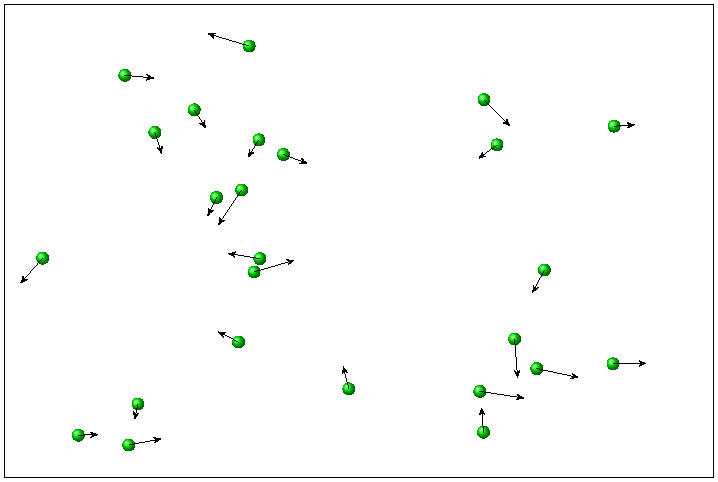
\includegraphics[width=6cm]{gas-random-motion}
		
	motion of gas molecules in a container
	
\end{wrapfigure}

gas consists of a large number of molecules

gas molecules move \emph{randomly} at high speeds

\cmt randomness results from \emph{collisions} of fast-moving molecules in the gas

for an individual molecule, its velocity changes constantly as it collides with other molecules

for the gas at any instant, there is a range of velocities for molecules

\cmt experimental evidence of random motion: \keypoint{Brownian motion}\index{Brownian motion}

dust or smoke particles in air undergo jerky random motion (viewed through microscope)

this is due to collisions with gas molecules that move randomly

\cmt speed of gas molecules depend on temperature

molecules move faster at higher temperature\footnote{We will prove this statement later in this chapter.}


\subsubsection{amount of molecules}

there are a huge number of molecules in a gas

we introduce \keypoint{amount of substance}\index{amount of substance} to measure the size of a collection of particles

\cmt unit of amount of substance: $[n] = \text{mol}$

\begin{ilight}
	one \keypoint{mole} is defined as the amount carbon-12 atoms in a sample of 12 grams
\end{ilight}

\cmt 1 mole of substance contains 6.02$\times$10$^{23}$ particles

this number is called \keypoint{Avogadro constant}\index{Avogadro constant}: $N_A = 6.02\times10^{23} \text{ mol}^{-1}$ \footnote{In 2018, IUPAC suggested a new definition of the mole, which is defined to contain exactly 6.02$\times$10$^{23}$ particles. This new definition fixed numerical value of the Avogadro constant, and emphasized that the quantity `amount of substance' is concerned with counting number of particles rather than measuring the mass of a sample.}

conversion between number of molecules and amount of substance: $\boxed{N=nN_A}$

\cmt it is useful to introduce the notion of molar mass $M$

\begin{ilight}
	\keypoint{molar mass}\index{molar mass} of a substance is defined as the mass of a given sample divided by the amount of substance: $M=\frac{m}{n}$
\end{ilight}

\begin{compactitem}
	\item[--] $\text{amount of substance} = \frac{\text{mass of sample}}{\text{molar mass}}$, or $n = \frac{m}{M}$
	
	\eqyskip
	
	\item[--] $\text{mass of single molecule} = \frac{\text{molar mass}}{\text{Avogadro constant}}$, or $m_0 = \frac{M}{N_A}$
\end{compactitem}

\example{Find the number of molecules in 160 grams of argon-40 gas.}

\sol amount of gas: $n=\frac{m}{M} = \frac{160 \text{ g}}{40 \text{ g mol}^{-1}} = 4.0 \text{ mol}$

number of gas molecules: $N = n N_A = 4.0 \text{ mol} \times 6.02\times10^{23} \text{ mol}^{-1} \approx 2.41 \times 10^{24}$ \eoe

\question{Find the mass of a sample of uranium-235 that contains $6.0\times10^{20}$ atoms.}
	




\subsubsection{pressure (qualitative view)}

when gas molecules collide with walls of container and rebound, they are acted by a force

by Newton's third law, gas molecules must exert a reaction force on container in return

contributions from many molecules give rise to a pressure

\example{If a gas is heated with its volume fixed, how does the pressure change?}

\sol at higher temperature, gas molecules move faster

they will collide \emph{harder} and produce a greater force upon each collision

they will also collide more \emph{frequently} with the container

so pressure of the gas will increase \eoe

\question{If you pump gas into a bicycle tyre, state and explain how the pressure changes.}

\question{A fixed amount of gas is allowed to expand at constant temperature, state and explain how the pressure changes.}



\subsection{ideal gas}

\subsubsection{ideal gas equation}

\rcyskip

\begin{ilight}
	a gas that satisfies the equation $\boxed{pV=nRT}$ or $\boxed{pV=NkT}$ at any pressure $p$, any volume $V$, and thermodynamic temperature $T$ is called an \keypoint{ideal gas}\index{ideal gas}
\end{ilight}

\keypoint{molar gas constant}: $R=8.31 \text{ J mol}^{-1}\text{ K}^{-1}$

\keypoint{Boltzmann constant}: $k=1.38\times10^{-23} \text{ J K}^{-1}$

values of $R$ and $k$ apply for any ideal gas, i.e., they are \emph{universal} constants

\cmt recall conversion between number of molecules and amount of substance: $\boxed{N=nN_A}$

we have relation between the constants: $R = kN_A$, or $k=\frac{R}{N_A}$

\cmt one must use \emph{thermodynamic temperature} in the equation

thermodynamic temperature is measured in kelvins (K), so it is also called the \emph{Kelvin scale}\footnote{We will discuss in details about Kelvin scale in \S\ref{s-temp-scale} and \S\ref{s-abs-zero}.}

conversion between Kelvin temperature and Celsius temperature: $\boxed{T_K (\text{K}) \text{ } \autorightleftharpoons{\footnotesize -273}{\footnotesize +273} \text{ } T_C (\OC)}$

\subsubsection*{real gases}

real gas behaves ideally at sufficiently high temperature and low pressure

\begin{compactitem}
	\item[--] at very low temperatures, real gas will condense into liquid or solid
	
	\item[--] at very high pressures, intermolecular forces become important
\end{compactitem}

however, under normal conditions (room temperature $T \approx 300 \text{ K}$ and standard atmospheric pressure $p \approx 1.0\times10^5 \text{ Pa}$), there is no significant difference between a real gas and an ideal gas

so ideal gas approximation can be used with good accuracy for most of our applications

\example{A sealed cylinder of volume of 0.050 m$^3$ contains 75 g of air. The molar mass of air is 29 g mol$^{-1}$. (a) Find the air pressure when its temperature is $30^\circ$C. (b) The gas is allowed to expand with its pressure fixed. Find the temperature of the gas when the volume doubles.}

\sol amount of gas: $n=\frac{m}{M} = \frac{75}{29} \approx 2.59 \text{ mol}$

\eqyskip

pressure at $30^\circ$C: $p = \frac{nRT_1}{V_1} = \frac{2.59\times8.31\times(30+273)}{0.050} \approx 1.30\times10^5 \text{ Pa}$

\eqyskip

pressure fixed, so $V \propto T \RA \frac{T_2}{T_1} = \frac{V_2}{V_1} = 2 \RA T_2 = 2\times (30+273) = 606 \text{ K} = 333^\circ\text{C}$ \eoe

\example{A gas cylinder holding 5000 cm$^3$ of air at a temperature of 27 $^\circ$C and a pressure of $6.0\times10^5 \text{ Pa}$ is used to fill balloons. Each balloon contains 1000 cm$^3$ of air at 27 $^\circ$C and $1.0\times10^5$ Pa when filled. (a) Find the initial amount of gas in the cylinder. (b) Find the number of balloons that can be filled.}

\sol initial amount of gas in cylinder: $n_0 = \frac{p_0 V}{RT} = \frac{9.0\times10^5\times5000\times10^{-6}}{8.31\times(27+273)} \approx 1.203 \text{ mol}$

\eqyskip

final amount of gas in cylinder: $n_\text{remain} = \frac{pV}{RT} = \frac{1.0\times10^5\times5000\times10^{-6}}{8.31\times(27+273)} \approx 0.201 \text{ mol}$\footnote{Air will leave the cylinder to fill balloons only if pressure inside the cylinder is higher than pressure of the balloon. When the two pressures become equal, no more balloons can be filled, there will be some air remain in cylinder.}

\eqyskip

amount of gas in each balloon: $n_\text{b} = \frac{pV_b}{RT} = \frac{1.0\times10^5\times1000\times10^{-6}}{8.31\times(27+273)} \approx 0.040 \text{ mol}$

\eqyskip

number of balloons: $N = \frac{n_0 - n_\text{remain}}{n_\text{b}} = \frac{1.203-0.201}{0.040} \approx 25$ \eoe

\example{A storage cylinder has a volume of $5.0\times10^{-4}\text{ m}^3$. The gas is at a temperature
	of 300 K and a pressure of $4.0 \times 10^6$ Pa.	(a) Find the number of molecules in the cylinder. (b) The gas molecules slowly leak from the cylinder at a rate of $1.6 \times 10^{16} \text{ s}^{-1}$. Find the time, in days, after which the pressure will reduce by 5.0\%.}

\sol initial number of molecules: $N_0 = \frac{p_0V}{kT} = \frac{4.0\times10^6\times 5.0\times10^{-4}}{1.38\times10^{-23}\times300}\approx 4.83\times10^{23}$

\eqyskip

volume fixed, so $N \propto p \RA \frac{\Delta N}{N_0} = \frac{\Delta p}{p_0} = 5.0\%$

number of molecules escaped: $\Delta N = 0.05\times4.83\times10^{23} \approx 2.42 \times10^{22}$

time needed: $t = \frac{2.42 \times10^{22}}{1.6 \times 10^{16}} \approx 1.51 \times 10^6 \text{ s} \approx 17.4 \text{ days}$ \eoe

\newpage %%%%

\question{Containers $A$ has a volume of $2.5\times10^{-2} \text{ m}^3$ contains a gas at a temperature of 17$^\circ$C and pressure of $1.3 \times 10^5 \text{ Pa}$ and . Another container $B$ of same size holds a gas at same temperature and a pressure of $1.9 \times 10^5 \text{ Pa}$. The two containers are initially isolated from each another. (a) Find the total amount of molecules. (b) The two containers are now connected through a tube of negligible volume. Assume the temperature stays unchanged, find the final pressure of the gas.}

\question{The air in a car tyre can be assumed to have a constant volume of $3.0\times10^{-2} \text{ m}^3$}. The pressure of this air is $2.8\times10^5 \text{ Pa}$ at a temperature of $25^\circ$C. The pressure is to be increased using a pump. On each stroke 0.015 mol of air is forced into the tyre. If gas has a final pressure of $3.6\times10^5 \text{ Pa}$ and final temperature of $28^\circ$C. Find the number of strokes of the pump required.


\subsubsection{empirical laws}

historically, the ideal gas law was first stated by \emph{\'Emile Clapeyron} in 1834:

for a fixed amount of gas, $\boxed{\frac{PV}{T} = \text{const}}$

his work was based on the empirical Boyle's law, Charles's law, and Gay-Lussac's law

we will next recover these laws from the ideal gas equation

\subsubsection*{Boyle's law}\index{Boyle's law}

Boyle's law was discovered by \emph{Robert Boyle} in 1662, based on experimental observations

\begin{wrapfigure}{r}{5cm}
	\centering
	\vspace*{-10pt}
		\begin{tikzpicture}[yscale=1.2]
		\draw [thick, <->] (0,4) node[left]{$p$} -- (0,0) node[below]{$0$} -- (4,0) node[below]{$V$};
		\draw [very thick,blue,domain=0.28:3.6,samples=20,smooth,variable=\x] plot (\x,{1/\x)});
		\draw (2.5,2) node{$pV=\text{const}$};
		\end{tikzpicture}
		\vspace*{-10pt}
\end{wrapfigure}

if temperature $T$ remains constant, then

{

\centering

$\boxed{pV=\text{const}}$, or $\boxed{p \propto \frac{1}{V}}$

} 

pressure $p$ of gas is inversely proportional to volume $V$

\cmt for a gas with fixed temperature: $p_1 V_1 = p_2 V_2$

\cmt a thermodynamic process for which temperature is kept constant is called an \emph{isothermal} process

$p$-$V$ relation for an isothermal process is shown




\subsubsection*{Charles's law}\index{Charles's law}

Charles's law was discovered by \emph{Jacques Charles} in 1787, based on experimental observations

\begin{figure}[ht]
	\centering
	\begin{tikzpicture}[scale=1.6]
		\draw [thick, ->] (-2.73,0.6) -- (-2.73,3) node[left]{$V$};
		\draw [thick, ->] (-3.2,0) -- (3,0) node[below]{$T_K/\text{K}$} node[above]{$T_C/\OC$};
		\draw [thick,blue,domain=-0.5:2.8,samples=2,smooth,variable=\x] plot (\x,{0.45*(\x+2.73)});
		\draw [thick,blue,dotted,domain=-2.73:-0.5,samples=2,smooth,variable=\x] plot (\x,{0.45*(\x+2.73)});
		\draw [thick,blue] (-0.5,1.0035) to [out=204.2,in=30] (-1.2,0.65) to [out=210,in=90] (-1.5,0.15);
		\draw[white,fill] (-2.3,0.2) rectangle (-1.8,0.5);
		\foreach \s in {-200,-100,...,200}
		\draw [thick] (\s/100,0) --(\s/100,0.1) node[above]{\s};
		\foreach \s in {0,100,...,500}
		\draw [thick] (\s/100-2.73,0) -- (\s/100-2.73,-0.1) node[below]{\s};
		\draw [thick] (-2.73,0) -- (-2.73,0.1) node[above]{-273};
		\draw [<-, thick] (-1.6,0.6) to [out=90, in=270] (-1,1.6) node[above]{ideal behaviour};
	\end{tikzpicture}
\end{figure}

if pressure $p$ remains constant, then: $\boxed{\frac{V}{T}=\text{const}}$, or $\boxed{V \propto T}$

i.e., volume $V$ of gas is directly proportional to its temperature $T$

\cmt proportionality relation only applies if Kelvin scale is used

\cmt a thermodynamic process for which pressure is kept constant is called an \emph{isobaric} process

$V$-$T$ relation for an isobaric process is shown

\cmt Charles's law implies that volume of gas tends to zero at a certain temperature

historically this is how the idea of \emph{absolute zero} first arose

\cmt as $T\to0$, a real gas condenses into solid

there will be deviation from ideal behaviour (dotted line)



\subsubsection*{Gay-Lussac's law}\index{Gay-Lussac's law}

\begin{wrapfigure}{r}{4.5cm}
	\centering
	\vspace*{-40pt}
	\begin{tikzpicture}[scale=1]
	\draw [thick, <->] (0,4) node[left]{$p$} -- (0,0) node[below]{$0$} -- (4,0) node[below]{$T$};
	\draw [thick,blue] (1,1) -- (3.6,3.6);
	\draw [thick,dotted] (0,0) -- (1,1);
	\end{tikzpicture}
	\vspace*{-30pt}
\end{wrapfigure}

Gay-Lussac's law was discovered by \emph{Joseph Louis Gay-Lussac} between 1800 and 1802


if volume $V$ remains constant, then

{
	
	\centering
	
	$\boxed{\frac{p}{T}=\text{const}}$, or $\boxed{p \propto T}$
	
} 

i.e., pressure $p$ is directly proportional to temperature $T$

\cmt a thermodynamic process for which volume is kept constant is called an \emph{isochoric} process, or \emph{isometric} process

$p$-$T$ relation for an isochoric process is shown

\cmt behaviour of real gas again deviates from ideal behaviour (dotted line) as $T\to0$





\subsection{kinetic theory of ideal gases}

\keypoint{kinetic model of gases}\index{kinetic model of gases}: a theory based on microscopic motion of molecules of a gas that explains its macroscopic properties

\subsubsection{assumptions of ideal gas model}

\rcyskip

\begin{ilight}
	
kinetic theory of the ideal gas model is based on the following assumptions:

\begin{compactitem}
	
\item[--] gas molecules are in constant \emph{random} motion
	
\item[--] \emph{intermolecular separation} is much greater than size of molecules

volume of molecules is negligible compared to volume occupied by gas

\item[--] \emph{intermolecular forces} are negligible

\item[--] collisions between molecules are perfectly \emph{elastic}, i.e., no kinetic energy lost

\item[--] molecules travel in straight line between collisions
\end{compactitem}

\end{ilight}

\example{A mass of 20 g helium-4 at a temperature of 37$^\circ$C has a pressure of $1.2\times10^5 \text{ Pa}$. Each helium-4 atom has a diameter of 280 pm. (a) Find the volume occupied by the gas and the volume of atoms in this gas. (b) Compare the two volumes, suggest whether this gas can be considered as an ideal gas.}

\sol number of helium molecules: $N = nN_A = \frac{m}{M} \times N_A = \frac{20}{4.0} \times 6.02\times10^{23} \approx 3.01\times10^{24} $

\eqyskip

volume of gas: $V_\text{gas} = \frac{NkT}{p} = \frac{3.01\times10^{24}\times1.38\times10^{-23}\times (37+273)}{1.2\times10^5} \approx 0.107 \text{ m}^3$

\eqyskip

volume of one atom: $V_\text{atom} = \frac{4}{3}\pi r^3 = \frac{4}{3} \pi\times(140\times10^{-12})^3 \approx 1.15\times10^{-29} \text{ m}^3$

volume of all atoms: $V_\text{atoms} = N V_\text{atom} = 3.01\times10^{24} \times 1.15\times10^{-29} \text{ m}^3 \approx 3.46 \times 10^{-5} \text{ m}^{3}$

$V_\text{gas} \gg V_\text{atoms}$, so this gas can approximate to an ideal gas \eoe


\subsubsection{pressure (quantitative view)}

we are ready to derive a formula for pressure due to ideal gas

pressure of gas is due to collision of gas molecules with container

let's first consider the effect of one single molecule moving in one dimension only, and then generalise the result to a gas containing $N$ molecules moving in all three dimensions



\begin{figure}[ht]
\centering
\begin{tikzpicture}[scale=1]
\coordinate (A) at (0,0); 
\coordinate (B) at (3,0);
\coordinate (C) at (4.5,1); 
\coordinate (D) at (1.5,1);
\coordinate (E) at (0,3); 
\coordinate (F) at (3,3);
\coordinate (G) at (4.5,4); 
\coordinate (H) at (1.5,4);
\draw [gray!20,fill] (A) -- (D) -- (H) -- (E) -- cycle;
\draw [thick] (B) -- (A) -- (E) -- (F) -- (B) -- (C) -- (G) -- (H) -- (E);
\draw [thick] (F) -- (G);
\draw [thick,dashed] (A) -- (D) -- (C);
\draw [thick,dashed] (D) -- (H);
\draw [thick,blue,->] (1.6,2.1) -- (0.9,2.1) to [out=180,in=90] (0.75,1.95)to [out=-90,in=180] (0.9,1.8) -- (2.4,1.8) node[below, pos=0.7]{$v$};
\shade [ball color = green] (1.8,2.1) circle [radius=0.1];
\draw [thick,<->] (0,-0.5) -- (1.5,-0.5) node[below]{$l$} -- (3,-0.5);
\node at (0.75,2.5) {{\Large $A$}};
\node[above] at (1.8,2.2) {{\footnotesize $m$}};
\end{tikzpicture}

one gas molecule moving in 1-D
\end{figure}

let's assume this single molecule only moves in $x$-direction (see figure)

change in momentum when colliding with wall: $\Delta P_x = mv_x - (-mv_x) = 2mv_x$\footnote{In this section we use $P$ for momentum of a particle and $p$ for pressure of a gas to avoid confusion.}

time interval between collisions: $\Delta t=\frac{2l}{v_x}$

average force acting: $F_x=\frac{\Delta P_x}{\Delta t} = \frac{2mv_x}{\tfrac{2l}{v_x}} = \frac{mv_x^2}{l}$

average pressure: $p_x=\frac{F}{A} = \frac{mv_x^2}{lA} = \RA p_x = \frac{mv_x^2}{V}$

generalisation to $N$ molecules moving in 3-D

\begin{compactitem}
	\item[--] $N$ molecules so $N$ times the contributions to pressure
	
	but there is a \emph{distribution} of speeds for $N$ molecules, so should take average of $v^2$
	
	\item[--] in three-dimensional space, we have: $v^2=v_x^2 + v_y^2 + v_z^2$
	
	but molecules have no preference in any specific direction, so: $\avg{v_x^2} = \avg{v_y^2} = \avg{v_z^2} = \frac{\avg{v^2}}{3}$
	
	pressure should be shared equally among three dimensions: $p=p_x=p_y=p_z$
		
\end{compactitem}


therefore we find the pressure of an ideal gas is given by: $\boxed{p = \frac{Nm\avg{v^2}}{3V}}$

\cmt $\avg{v^2}$ is the \emph{mean square velocity} of gas molecules

we can further define r.m.s. (root mean square) velocity: $v_\text{rms} = \sqrt{\avg{v^2}}$ 

gas molecules in random motion so there exists a range of velocities

we cannot tell exact velocity of a specific molecule, but can only tell mean values

\cmt $N$ is number of molecules, $m$ is mass of one molecule

then $Nm$ gives total mass of the gas, and $\frac{Nm}{V}$ gives gas density $\rho$

we can rewrite the pressure formula as: $\boxed{p=\frac{1}{3}\rho \avg{v^2}}$ 

(pressure depends only on density and mean square speed of molecules)

\cmt physical interpretation of the formula

\begin{compactitem}
\item[--] $N \up$ $\ra$ more molecules, more collisions $\ra p\up$

\item[--] $m \up$ $\ra$ greater mass, greater force upon collision $\ra p\up$

\item[--] $v \up$ $\ra$ strike container harder, also more often $\ra p\up$

\item[--] $V \up$ $\ra$ spend more time in gas, less frequent collision with container $\ra p\down$
\end{compactitem}


\subsubsection{kinetic energy}

we now have two equations for ideal gases:
\begin{equation*}
\left\{
	\begin{array}{ll}
	pV = nRT \, \text{, or } \, pV = NkT &\quad \text{ideal gas law} \\
	p = \frac{Nm\avg{v^2}}{3V} &\quad \text{pressure law}
	\end{array} \right.
\end{equation*}

compare the two equations: $pV=\frac{1}{3}Nm\avg{v^2}=NkT \RA m\avg{v^2}=3kT$

\emph{mean kinetic energy} of a single molecule in a gas is: $\boxed{\avg{E_k}=\frac{1}{2}m\avg{v^2}=\frac{3}{2}kT}$

mean K.E. of ideal gas molecules is \emph{proportional} to its thermodynamic temperature

\cmt useful relation for molecular speeds: $\boxed{v_\text{rms}^2 \propto T}$

recall our statement in \S\ref{s-gas-intro}, higher temperature means higher speed for molecules

\cmt we only talk about \emph{translational} K.E. here

molecules have this energy because they are moving through space

total kinetic energy may also include \emph{rotational} K.E. and \emph{vibrational} K.E.
\footnote{There is an important result in classical thermal physics, known as the \emph{equipartition of energy theorem}. It states that the average energy per molecule is $\frac{1}{2}kT$ for each independent \emph{degree of freedom}. A molecule can move in three directions, corresponding to three translational degrees of freedom, thus its mean translational kinetic energy is $\frac{3}{2}kT$. For a polyatomic gas (each molecule consists of several atoms), apart from translational motion , it has additional rotational degrees of freedom and different vibrational modes, so its average energy can be calculated by counting the total number of degrees of freedom.}

\cmt $\avg{E_k} = \frac{3}{2}k T$ gives the \emph{mean}, or \emph{average} K.E. per molecule

gas molecules exchange energies with each other upon collisions

for an individual molecule, its K.E. is not a constant

but mean K.E. is constant, which depends on temperature $T$ only

\cmt in a mixture of several gases, K.E. is shared \emph{equally} among its components

this is because of repeated collisions between particles

though all molecules have same K.E., heavier molecules will move more slowly




\example{Air consists of oxygen (O$_2$, molar mass $32\text{ g mol}^{-1}$) and nitrogen (N$_2$, molar mass $28\text{ g mol}^{-1}$). (a) Calculate the mean translational kinetic energy of these molecules at 300 K. (b) Estimate the typical speed for each type of the molecule.}

\sol mean K.E. of single molecule: $\avg{E_k} = \frac{3}{2}kT = \frac{3}{2} \times 1.38\times10^{-23} \times 300 \approx 6.21\times 10^{-21} \text{ J}$

{
	
	\centering
	
	$\avg{E_k} = \frac{1}{2}m\avg{v^2} = \frac{3}{2} kT \RA \frac{1}{2} \frac{M}{N_A} \avg{v^2} = \frac{3}{2} kT \RA \avg{v^2} = \frac{3kN_AT}{M} = \frac{3RT}{M}$
	
}

\eqyskip

for oxygen molecule: $v_\text{O$_2$} \approx  \sqrt{\frac{3\times8.31\times300}{0.032}} \approx 483 \mps$

\eqyskip

for nitrogen molecule: $v_\text{N$_2$} \approx  \sqrt{\frac{3\times8.31\times300}{0.028}} \approx 517 \mps$ \eoe

\example{A cylinder container initially holds a gas of helium-4 at a temperature of 54\OC. (a) Find the mean square speed of these helium atoms. (b) If the temperature is raised to 540\OC, find the r.m.s. speed of the atoms.}

\sol mass of one helium-4 atom: $m=4\text{u} = 4\times 1.66\times10^{-27} \approx 6.64\times10^{-27} \text{ kg}$

at 54\OC: $\, \frac{1}{2}m\avg{v^2} = \frac{3}{2}kT \RA \avg{v^2} = \frac{3kT}{m} = \frac{3\times1.38\times10^{-23}\times(54+273)}{6.64\times10^{-27}} \approx 2.04 \times 10^6 \text{ m}^2 \text{ s}^{-2}$

\eqyskip 

note relation between $v$ and $T$: $\, \avg{v^2} \propto T \RA \frac{\avg{v^{\prime 2}}}{\avg{v^2}} = \frac{T'}{T} \RA v'_\text{rms} = \sqrt{\frac{T'}{T}}\times v_\text{rms}$

\eqyskip 

at 540\OC: $\, v'_\text{rms} = \sqrt{\frac{540+273}{54+273}} \times \sqrt{2.04 \times 10^6} \approx 2.25 \times 10^3 \mps$ \eoe


\question{A fixed mass of gas expands to twice its volume at constant temperature. (a) How does its pressure change? (b) How does mean kinetic energy change?}

\question{In order for a molecule to escape from the gravitational field of the earth, it must have a speed of $1.1\times10^6\mps$ at the top of the atmosphere. (a) Estimate the temperature at which helium-4 atoms could have this speed. (b) Helium atom actually escape from top of the atmosphere at much lower temperatures, explain how this is possible.}
\section{Thermodynamics}


\subsection{thermal physics basics}


\subsubsection{temperature scales}\label{s-temp-scale}

\begin{wrapfigure}{r}{6cm}
	\centering
	\vspace*{-2.7cm}
	\begin{tikzpicture}[yscale=1.6]
	\draw[->] (0,-3) -- (0,1.50);
	\foreach \temp in {-2.73,-1.96,0,0.25,1.00} \draw (-0.1,\temp) --++ (0.2,0);
	\node[left] at (-0.2,1.5) {$T_C(\OC)$};
	\node[right] at (0.2,1.5) {$T_K(\text{K})$};
	\node[left] at (-0.2,-2.73) {-273\OC};
	\node[left] at (-0.2,-1.96) {-196\OC};
	\node[left] at (-0.2,-0) {0\OC};
	\node[left] at (-0.2,0.25) {25\OC};
	\node[left] at (-0.2,1) {100\OC};
	\node[right] at (0.2,-2.73) {0 K};
	\node[right] at (0.2,-1.96) {77 K};
	\node[right] at (0.2,-0) {273 K};
	\node[right] at (0.2,0.25) {298 K};
	\node[right] at (0.2,1) {373 K};
	\node[right] at (1.35,-2.73) {absolute zero};
	\node[right] at (1.35,-1.96) {liquid nitrogen};
	\node[right] at (1.35,0) {ice-water mixture};
	\node[right] at (1.35,0.25) {room temperature};
	\node[right] at (1.35,1.00) {boilng water};
	\end{tikzpicture}
	\vspace*{-30pt}
\end{wrapfigure}

\cmt Celsius scale (unit: \OC)

0$^\circ$C defined as temperature of ice-water mixture

100$^\circ$C defined as temperature of boiling water

\cmt Kelvin scale (unit: K)

0 K (\emph{absolute zero}) is lowest temperature possible

\cmt conversion rule: $T_K (\text{K}) \text{ } \autorightleftharpoons{\footnotesize -273}{\footnotesize +273} \text{ } T_C (\OC)$

\cmt change of 1$^\circ$C equals change of 1 K


\subsubsection{kinetic theory of matter}

there are three common states of matter: solid, liquid and gas

they have very different physical properties (density, compressibility, fluidity, etc.)

but deep down, they are all composed of a large number of small molecules

in the \keypoint{kinetic theory of matter}, we look at microscopic behaviour at molecular level (arrangement, motion, intermolecular forces, separation, etc.)

\emph{microscopic} behaviour of molecules cause differences in \emph{macroscopic} properties of matter

\begin{compactitem}
	\item[--] solid: molecules close together, tightly bonded, vibrate about their positions
	
	\item[--] liquid: molecules quite close together, vibrate but has some freedom to move about
	
	\item[--] gas: molecules widely separated, free from neighbours, move rapidly
\end{compactitem}

\subsubsection{specific latent heat}

it requires heat energy to \emph{melt} a solid or \emph{boil} a liquid

melting and boiling usually occur at a fixed temperature

thermal energy to cause the change of state at a constant temperature is called \emph{latent heat}

amount of latent heat needed depends on mass of substance: $\boxed{Q=Lm}$

\begin{ilight}
	we define \keypoint{specific latent heat}\index{specific latent heat} ($L$) as the thermal energy required to change the state of \emph{unit} mass of substance with no change in temperature is called 
\end{ilight}



\cmt unit of specific latent heat: $[L] = \text{J}\cdot\text{kg}^{-1}$

\cmt specific latent heat is an \emph{intensive} property

i.e., $L$ does not depend on size or shape of sample, $L$ depends on type of substance only 
	
\cmt for melting, $L$ is called \emph{specific latent heat of fusion}
	
for boiling, $L$ is called \emph{specific latent heat of vaporisation}
	
\cmt latent heat is related to breaking bonds and increasing intermolecular separation
	
vaporisation requires larger increase in particle separation than fusion
	
for a given substance, $L_\text{vapour}>L_\text{fuse}$


\example{A 3.0 kW electric kettle contains 0.5 kg of water already at its boiling point. Neglecting heat losses, determine how long it takes to boil dry. ($L_\text{water} = 2.26 \times 10^6 \text{ J kg}^{-1}$)}
	
\sol heat required: $Q=mL = 0.50 \times 2.26 \times 10^6 = 1.13 \times 10^6 \text{ J}$
	
time needed: $t=\frac{Q}{P} = \frac{1.13 \times 10^6}{3.0\times 10^3} \approx 380 \text{ s} \approx 6.3 \text{ min}$ \eoe
 
\example{A student measures specific latent heat of fusion for ice. He uses an electric heater to melt ice but the insulation is not perfect. The experiment is carried out twice, with the heater operating at different powers. Use the data table to calculate specific latent heat of fusion.}

\begin{center}
	\begin{tabular}{|C{1.6cm}|C{2cm}|c|c|}
		\hline  & Power (W) & time interval (min) & mass of ice melted (g) \\ 
		\hline test 1 & 60 & 3.0 & 40.4 \\ 
		\hline test 2 & 90 & 3.0 & 56.6 \\ 
		\hline 
	\end{tabular} 
\end{center}

\sol there exists heat gain from surroundings, so effective power $P_\text{eff}=P_\text{heater}+P_\text{sur}$

heat energy to melt ice: $Q = mL = (P_\text{heater}+P_\text{sur}) t$
\begin{equation*}
	\left\{ \begin{array}{l}
		40.4 \times L = (60+P_\text{sur})\times3.0\times60 \\
		56.6 \times L = (90+P_\text{sur})\times3.0\times60 
	\end{array}\right.
	\RA \left\{ \begin{array}{l}
	L \approx 333 \text{ J g}^{-1} \\
	P_\text{sur} \approx 14.8 \text{ W} \end{array}\right. \teoe
\end{equation*}

\eqyskip

\question{A student designs an experiment to determine the specific latent heat of fusion $L$ of ice. Some ice at $0\OC$ is heated with an electric heater. The experiment is carried out twice and the following data are obtained.
	
\begin{center}
	\begin{tabular}{|c|c|c|c|}
		\hline  & energy supply from heater (J) & time interval (min) & mass of ice melted (g) \\ 
		\hline heater off & 0 & 10.0 & 14.3 \\ 
		\hline heater on & 21000 & 5.0 & 70.0 \\ 
		\hline 
	\end{tabular} 
\end{center}

(a) Suggest why two sets of readings are taken. (b) Find specific latent heat of fusion for ice.}

\subsubsection{specific heat capacity}

heating a substance could cause an increase in its temperature

heat required is proportional to its mass $m$ and temperature change $\Delta T$: $\boxed{Q=cm\Delta T}$

\begin{ilight}
	we define \keypoint{specific heat capacity }\index{specific heat capacity} ($c$) as the thermal energy required per unit mass of substance to cause an increase of one unit in its temperature
\end{ilight}


\cmt unit of specific heat capacity: $[c] = \text{J kg}^{-1} \text{ K}^{-1}$ or J kg$^{-1}$ $^\circ\text{C}^{-1}$
	
\cmt $c$ is also an \emph{intensive} property, i.e., independent of size or shape of the sample


\example{A block of 30 g ice at $-20^\circ$C is added to a large cup of 270 g water at 80$^\circ$C. Assume there is no energy lost, what is the final temperature of the mixture? (data: specific heat capacity of water is 4200 J kg$^{-1}$ K$^{-1}$, specific heat capacity of ice is 2100 J kg$^{-1}$ K$^{-1}$, specific latent heat of ice is $3.3\times10^5$ J kg$^{-1}$.}

\sol energy lost by hot water = energy gain by ice cube
\begin{equation*}
	\underbrace{4200\times0.27\times(80-T)}_{\text{95 $^\circ\text{C}$ water $\to T$ $^\circ\text{C}$  water}} = 
	\underbrace{2100\times0.030\times[0-(-20)]}_{-\text{20 $^\circ\text{C}$ ice $\to 0$ $^\circ\text{C}$  ice}} +
	\underbrace{3.3\times10^5\times0.030}_{\text{0 $^\circ\text{C}$ ice $\to 0$ $^\circ\text{C}$ water}} + 
	\underbrace{4200\times0.030\times(T-0)}_{\text{0 $^\circ\text{C}$ water $\to T$ $^\circ\text{C}$  water}}
\end{equation*}

\vspace*{-1em}
\begin{equation*}
	90720 - 1134T = 1260 + 9900 + 126 T
\end{equation*}
\begin{equation*}
	T = \frac{90720-1260-9900}{1134+126} \approx 63 ^\circ\text{C} \teoe
\end{equation*}


\example{A 1.00 kg aluminium block is heated using an electrical heater. The current in the heater is 4.2 A and the p.d. across is 12 V. Measurements of the rising temperature are represented by the graph. Determine specific heat capacity  of aluminium.}

\begin{figure}[ht]
	\centering
	\begin{tikzpicture}[scale=1]
	\draw[style=help lines,step=0.5,gray!50] (0,0) grid (7.5,5.5);
	\draw [thick, ->] (-0.5,0) --(8,0) node[below]{$t/\text{s}$};
	\draw [thick, ->] (0,-0.5) --(0,6) node[left]{$T/\OC$};
	\foreach \s in {100,200,...,700}
	\draw [very thick] (\s/100,-0.1) -- (\s/100,0) node[below]{\s} -- (\s/100,0.1);
	\foreach \s in {10,20,...,50}
	\draw [very thick] (-0.1,\s/10) -- (0,\s/10) node[left]{\s} -- (0.1,\s/10);
	\draw [very thick,blue] (0,2) -- (7.5,5.075);
	\draw [very thick,red] (0,2) -- (5.5,2) node[midway,below]{\textcolor{black}{$\Delta t = 550 \text{ s}$}} -- (5.5,4.255) node[right,midway]{\textcolor{black}{$\Delta T = 22.5 \OC$}};
	\foreach \s in {0,1,...,7}
	\draw [fill] (\s,2+0.41*\s) circle(0.05);
	\end{tikzpicture}
\end{figure}

\sol energy supplied: $Q = cm\Delta T \RA IV\Delta t = cm\Delta T \RA c = \frac{IV}{m \tfrac{\Delta T}{\Delta t}} $

$\frac{\Delta T}{\Delta t}$ is gradient of fitting line: $\frac{\Delta T}{\Delta t} = \frac{22.5}{550} \approx 4.09 \times 10^{-2} \text{ } \OC \text{ s}^{-1}$

specific heat capacity: $c = \frac{4.2\times12}{1.00 \times 4.09 \times 10^{-2}} \approx 1230 \jpkgC$	\eoe

\question{A mixture contains 5\% silver and 95\% of gold by weight. Some gold is melted and the correct weight of silver is added. The initial temperature of silver is $20^\circ$C. Use the data to calculate the initial temperature of gold so that the final mixture is at melting point of gold.}

\begin{center}
	\begin{tabular}{|l|c|c|}
		\hline  & silver & gold \\ 
		\hline melting point (K) & 1240 & 1340 \\ 
		\hline specific heat capacity (solid or liquid) (J kg$^{-1}$ K$^{-1}$) & 235 & 129 \\ 
		\hline specific latent heat of fusion (kJ kg$^{-1}$) & 105 & 628 \\
		\hline 
	\end{tabular} 
\end{center}



\subsection{internal energy}

we now consider the total energy within a thermodynamic system

molecules in a system undergo random motion, so they have kinetic energy

there are potential energy between molecules due to intermolecular interaction

\begin{ilight}
	\keypoint{internal energy}\index{internal energy} is defined as the sum of random kinetic energy of molecules and potential energy between molecules: $\boxed{U=E_k+E_p}$
\end{ilight}

\cmt internal energy is a \emph{state function} of the system

it only depends on current state of system, not on process to arrive at this state

\subsubsection{kinetic energy}

\cmt internal energy counts K.E. due to random motion at molecular level

K.E. of macroscopic motion of the system as a whole is not included

\cmt mean K.E. of molecules is directly proportional to temperature: $\boxed{E_k \propto T}$

K.E. of molecules depends on temperature only

higher temperature means molecules move faster, vibrate more intensively, etc.





\subsubsection{potential energy}

\cmt internal energy counts P.E. due to force fields \emph{within} the system

P.E. of the system as a whole due to \emph{external} force fields is not included

\cmt P.E. between molecules depends on intermolecular separation and chemical bonding

in general, greater intermolecular separation means greater P.E.\footnote{Intermolecular separation does not necessarily increase during melting processes. A typical counter example is melting of ice into water, for which intermolecular separation actually decreases (density of water > density of ice), but potential energy of the system will still increase because hydrogen bonds between H$_2$O molecules are broken.}: $\boxed{r \up \Leftarrow E_p \up}$

breaking intermolecular bonds also causes an increase in P.E.

mean P.E. of gas $>$ mean P.E. of liquid $>$ mean P.E. of liquid solid

\subsubsection{internal energy of ideal gas}

for ideal gas, mean K.E. of one molecule: $E_k = \frac{3}{2}kT$

there is no intermolecular force, so P.E. of ideal gas is defined to be zero: $E_p = 0$

internal energy per molecule: $U = E_k + E_p = \frac{3}{2}kT$

hence internal energy of ideal gas is purely kinetic and directly proportional to temperature

total internal energy of the gas: $U_\text{gas} = NU \RA \boxed{U_\text{gas} = \frac{3}{2}NkT}$

\subsubsection{change of states}

consider a substance being heated from its solid state

it will melt into a liquid and further vaporise into its gaseous state

we now look into the changes of internal energy during each stage

\begin{figure}[ht]
\centering
\begin{tikzpicture}[scale=1]
\draw[thick,->] (-1,-2) -- (0,-2) -- (10,-2) node[below] {$t$};
\draw[thick,->] (0,-2.5) -- (0,5) node[left]{$T$};
\draw [very thick,blue] (0,-1) node[left]{$A$} -- (1,0) node[above]{$B$} -- (2.5,0) node[above left]{$C$} -- (4,3) node[above]{$D$} -- (9,3) node[above left]{$E$} -- (9.5,4.5) node[above]{$F$};
\draw[thick,dashed] (4,3) -- (0,3) node[left]{$T_\text{boiling}$};
\draw[thick,dashed] (1,0) -- (0,0) node[left]{$T_\text{melting}$};
\end{tikzpicture}
\end{figure}


\begin{compactitem}
\item[--] $AB$ (solid state): $T \up \ra E_k \up$, greater vibration for solid particles

but no (significant) change in mean separation\footnote{A typical solid material expands when it is heated, so intermolecular separation will increase slightly.} $\ra$ no change in P.E.

\item[--] $BC$ (\emph{melting}): latent heat goes into breaking intermolecular bonds, $r\up \ra E_p \up$

but melting occurs at constant temperature\footnote{Here we talk about \emph{pure substance}, which changes from solid into liquid at a particular temperature, called the \emph{melting point}. But for a \emph{mixture} of substances, melting may occur over a \emph{range} of temperatures. It is also possible for a substance to decompose before they change states.} $\ra$ no change in K.E.

\item[--] $CD$ (liquid state): $T \up \ra E_k \up$, greater vibration and free motion

but no (significant) change in mean separation $\ra$ no change in P.E.

\item[--] $DE$ (\emph{boiling}): molecules break free, $r\up \ra E_p \up$

boiling occurs at constant temperature\footnote{Again we only concern pure substances. Mixtures that boil over a range of temperatures or substance decompose before phase transition are not considered here.} $\ra$ no change in K.E.

\item[--] $EF$ (gas state): $T \up \ra E_k \up$ particles move even faster

particles completely separated, no intermolecular force, so constant $E_p = 0$
\end{compactitem}

\question{For a particular substance, why is the specific latent heat of vaporisation much greater than the specific latent heat of fusion?}

\subsubsection*{evaporation}

liquid changes into gas without boiling $\longrightarrow$ \keypoint{evaporation}\index{evaporation}

particles move randomly, i.e., they move at various speeds

some molecules move fast enough to break free

\cmt \emph{cooling effect}: evaporation causes a decrease in temperature of the liquid

most energetic molecules escaped, those remain in the liquid have less energy, $E_k \down \ra T \down$

\cmt rate of evaporation increases with temperature, surface area of liquid

\cmt different between boiling and evaporation

\begin{center}
	\begin{tabular}{|c|c|c|}
		\hline 
		& boiling & evaporation \\ 
		\hline 
		occurrence & throughout the liquid & at surface only \\ 
		\hline 
		temperature & occur at boiling point & occur at any temperature \\ 
		\hline 
		bubble formation & bubbles formed & no bubbles \\ 
		\hline 
		rate of process & fast & slow \\ 
		\hline 
	\end{tabular} 
\end{center}

\subsubsection{first law of thermodynamics}

internal energy of a system changes upon heat transfer or doing work

\begin{ilight}
	\keypoint{first law of thermodynamics}\index{law of thermodynamics!first law of thermodynamics} states that the increase in internal energy equals sum of heat supply to the system and work done on the system: $\boxed{\Delta U = Q +  W}$
\end{ilight}

\cmt first law of thermodynamics is an extension of the law of conservation of energy

\cmt sign conventions for $Q$ and $W$

\begin{compactitem}
	\item[$\circ$] $Q>0$ if heat supplied to system
	
	\item[$\circ$] $Q<0$ if heat released by system to surroundings
	
	\item[$\circ$] $W>0$ if work done \emph{on} system by external
	
	i.e., if system is compressed and volume decreases, then $W>0$
	
	\item[$\circ$] $W<0$ if system does work \emph{against} surroundings
	
	i.e., system expands and volume increases, then $W<0$
	
\end{compactitem}

\cmt amount of heat energy: $Q=\left\{ \begin{array}{l}
	cm\Delta T \qquad (\text{if no change of state}) \\
	Lm \qquad (\text{during change of state})
	\end{array}\right.$

\cmt amount of work is related to pressure and change of volume

if volume changed at \emph{constant} pressure, then $W=F\Delta s = pA\Delta s \ra \boxed{W = p\Delta V}$\footnote{If pressure changes with volume during a thermodynamics process, then work done $W=\int p \dd V$. Alternatively, we can evaluate the area under a $p$-$V$ graph to find the work done.}

if no change of volume, then no work is done
	

\example{A gas is heated by supplying it with 25 kJ of energy. The gas expands so that the volume increases by 0.10 m$^3$. Assume the gas has a fixed pressure of 150 kPa during the process. Calculate the change in internal energy.}

\sol amount of work done: $W = p \Delta V = 150 \times 0.10 = 15 \text{ kJ}$

but gas expands means work is done against surroundings, so this is negative work

change in internal energy: $\Delta U = Q +  W = (+25) + (-15) = +10 \text{ kJ}$ \eoe

\example{Use the idea of internal energy and the first law of thermodynamics, explain why boiling water requires heat supply.}

\sol boiling occurs at constant temperature, so $\Delta E_k = 0$

but separation between molecules increased, so $\Delta E_p >0$

by definition, internal energy $U=E_k+E_p$, so $\Delta U >0$

during boiling, there is an increase in volume, so work against surroundings, $W<0$

recall first law of thermodynamics $\Delta U = Q + W$, must have $Q>0$

this means heat must be supplied for boiling processes \eoe

\example{When you pump up a bicycle tyre, the temperature of air inside the tyre will go up. Explain why this happens using the first law of thermodynamics.}

\sol pumping up tyre involves compressing gas, so positive work is done: $W>0$

for each stroke, there is little time for heat transfer, so $Q \approx 0$

according to first law of thermodynamics $\Delta U = Q + W \RA \Delta U >0$

by definition, internal energy $U=E_k + E_p \RA \Delta U = \Delta E_k + \Delta E_p>0$

but for gas, there is negligible intermolecular force, so $\Delta E_p=0$, then must have $\Delta E_k>0$

K.E. of molecules is proportional to temperature, higher K.E. so higher temperature \eoe

\example{An ideal gas of 0.080 mol is initially at state $A$ and then undergoes a cycle $ABCA$. The variation of its pressure $p$ with its volume $V$ is shown on the graph.}

\begin{figure}[ht]
	\centering
	\begin{tikzpicture}[scale=0.9]
	\draw[<->] (0,7.5) node[left]{$p$/kPa} -- (0,0) -- (7.5,0) node[below] {$V/10^{-2}$ m$^3$};
	\draw[help lines, gray] (0,0) grid (7,7);
	\foreach \x in {0,100,200,300} \node[left] at (-0.1,\x*2/100) {$\x$};
	\foreach \x in {0,2,4,6} \node[below] at (\x,-0.1) {$\x$};
	\draw[very thick, blue, ->] (2,2) node[below left]{$A$} -- (2,4.5);
	\draw[very thick, blue] (2,4.5) -- (2,6) node[above left]{$B$};
	\draw [very thick, blue, domain=2:6] plot (\x, {12/\x}) node[below right]{$C$};
	\draw[very thick, blue, ->] (6,2) -- (3.5,2);
	\draw[very thick, blue] (3.5,2) -- (2,2);
	\draw[very thick, blue, ->] (4.5,2.67) -- (4.55,2.64);
	\end{tikzpicture}
\end{figure}

Temperature of state $A$ is 300 K. The magnitude of work on gas from state $B$ to $C$ is 6570 J.

For each stage $A \to B$, $B \to C$ and $C \to A$ during the cycle, determine work done and heat supply to the gas, and also find the change in internal energy.

\newpage

\sol work done depends on change in volume

$A\to B$: no change in volume, so $W_{AB} = 0$

$B \to C$: $|W_{BC}|= 6570 \text{ J}$, but expansion implies $W<0$, so $W_{BC}=-6570 \text{ J}$

$C \to A$: $|W_{CA}| = p\Delta V_{CA} = 1\times10^5 \times (6-2)\times10^{-2} \RA W_{CA}= +4000 \text{ J}$ (compression so $W>0$)

\noindent change in internal energy of ideal gas depends on change in temperature

$A\to B$: same $V$ but $p_B = 3p_A$, so $T_B = 3T_A = 900 \text{ K}$

$\phantom{A\to B\text{: }}\Delta U_{AB} = \frac{3}{2}Nk\Delta T_{AB} = \frac{3}{2}\times 0.80\times 6.02\times10^{23}\times1.38\times10^{-23}\times(900-300) \approx +5980 \text{ J}$

$B \to C$: note that $p_BV_B = p_CV_C$, so $T_B = T_C$, no change in temperature, so $\Delta U_{BC}=0$

$C \to A$: $\Delta U_{CA} = \frac{3}{2}Nk\Delta T_{CA} = \frac{3}{2}\times 0.80\times 6.02\times10^{23}\times1.38\times10^{-23}\times(300-900) \approx -5980 \text{ J}$


for cycle $ABCA$, same initial and final state, so total change in internal energy must be zero

one can check that $\Delta U_\text{cycle} = \Delta U_{AB} + \Delta U_{BC} + \Delta U_{CA} = 0$
	
\noindent to find supply of thermal energy, we apply first law of thermodynamics: $\Delta U = Q + W$

$A\to B$: $+5980 = Q_{AB} + 0 \RA Q_{AB} = +5980 \text{ J}$

$B \to C$: $0 = Q_{BC} + (-6570) \RA Q_{BC} = +6570 \text{ J}$

$C \to A$: $-5980 = Q_{CA} + (+4000) \RA Q_{CA} = -9980 \text{ J}$

\noindent the table below summarises all energy changes during the cycle $ABCA$
\begin{center}
		\begin{tabular}{|C{2.5cm}|C{2.5cm}|C{2.5cm}|C{2.5cm}|}
			\hline
			change &  $W$/J & $Q$/J & $\Delta U$/J \\ \hline
			$A \to B$ & 0 & +5980 & +5980\\ \hline
			$B \to C$ & -6570 & +6570 & 0 \\ \hline
			$C \to A$ & +4000 & -9980 & -5980 \\ \hline
		\end{tabular}
	
	\vspace*{-0.1\baselineskip}\eoe
\end{center}

\question{Show that when $n$ mol of gas is heated at a fixed volume, thermal energy required to raise the temperature by 1.0 K is $nR$.}

\question{Two identical balloons $A$ and $B$ hold the same amount of gas at the same initial temperature. They are given the same amount of heat. Suppose volume of $A$ is fixed, while $B$ is allowed to expand, compare the final temperatures of the gases in the two balloons.}


\subsection{temperature}

\subsubsection{temperature \& thermal energy}

\cmt temperature can be considered as a \emph{relative} measure of thermal energy

temperature can tell the \emph{direction} of thermal energy flow

heat always (spontaneously) flows from high temperature regions to colder regions\footnote{This is the consequence of the \emph{second law of thermodynamics}\index{law of thermodynamics!second law of thermodynamics ($\star$)}, which is concerned with the direction of natural processes. The law states that the total \emph{entropy}, a quantity that counts the number of microstates of a system, of an isolated system can never decrease over time. You will learn more about entropy if you study A-Level chemistry.}

\cmt if two objects in contact have the same temperature, then there is no net heat transfer

the two objects are said to be in \keypoint{thermal equilibrium}\index{thermal equilibrium}

\cmt if two systems $A$ and $B$ are each in thermal equilibrium with a third system $C$, $A$ and $B$ are also in thermal equilibrium, this is called the \keypoint{zeroth law of thermodynamics}\index{law of thermodynamics!zeroth law of thermodynamics}
\footnote{This law is important for the formulation of thermal physics. The physical meaning of the law was expressed by Maxwell: "All heat is of the same kind." The zeroth law allows us to give the mathematical definition of temperature.}

\question{A student thinks that temperature measures the amount of heat in an object. Suggest why this statement is incorrect with examples.}

\subsubsection{absolute zero}\label{s-abs-zero}

mean K.E. of molecules is a microscopic description of temperature $T$

minimum K.E. occurs if molecules do not move at all (completely frozen)\footnote{In the \emph{classical} description, there is no reason not allowing a molecule to cease motion. However, due to \emph{quantum mechanical effects}, kinetic energy of a system cannot be zero even at absolute zero.}

this corresponds to the lowest possible temperature, called \keypoint{absolute zero}\index{absolute zero}

\cmt \keypoint{Kelvin scale of thermodynamic temperature} is defined based on absolute zero as 0 K\footnote{More precisely, 0 K for absolute zero  and $273.16\text{ K}$ for water triple point.}

\cmt conversion rule between Celsius scale and Kelvin scale: $\boxed{T_K (\text{K}) \text{ } \autorightleftharpoons{\footnotesize -273.15}{\footnotesize +273.15} \text{ } T_C (\OC)}$\footnote{The numerical value of 273.15 will only be quoted in this section. For everywhere else in the notes, we will use the less precise value 273 for simplicity.}

\cmt Kelvin scale is said to be an \emph{absolute scale}

zero of Kelvin scale does not depend on property of a specific substance

in contrast, zero of Celsius scale is based on properties of water

\cmt it is impossible to remove any more energy from a system at 0 K (or -273.15 \OC)

but there is no practicable means to bring a physical system to exactly $0\text{ K}$
\footnote{This is known as the \emph{third law of thermodynamics}\index{law of thermodynamics!third law of thermodynamics ($\star$)}, which states that it is impossible, no matter how idealized, to reduce the temperature of any closed system to absolute zero in a finite number of operations.}




\subsubsection{thermometer}

a \keypoint{thermometer}\index{thermometer} is a device which can be used to measure temperature



\subsubsection*{liquid-in-glass thermometer}

basic principle: liquid expands in volume at higher temperature

examples include alcohol thermometer, mercury-in-glass thermometer, etc.

\begin{center}
	\begin{tikzpicture}[scale=1.35]
		\draw[red!50,fill] (45:0.6) arc(45:315:0.6) [out=45, in=180] to (0.8,-0.3) -- (4,-0.3) -- (4,0.3) -- (0.8,0.3) [out=180, in=-45] to (45:0.6);
		\draw[ultra thick] (45:0.6) arc(45:315:0.6) [out=45, in=180] to (0.8,-0.3) -- (8,-0.3) arc(-90:90:0.3) -- (0.8,0.3) [out=180, in=-45] to (45:0.6);
		\draw[thick] (1,0) -- (7.67,0);
		\foreach \temp in {0,10,20,...,100}{
			\draw[thick] (1+\temp/15,-0.15) --++ (0,0.3);
			\node[below] at (1+\temp/15,-0.3) {{\scriptsize \temp\OC}};
		}
	\end{tikzpicture}
\end{center}

\subsubsection*{resistance temperature detectors (RTD)}

basic principle: resistance of electronic element changes with temperature

metal wires and thermistor are both used in RTD elements 


\subsubsection*{thermocouple}\index{thermocouple}

basic principle: difference in temperature can produce a \emph{thermoelectric voltage} across junctions, thermocouple measures temperatures by means of this voltage

\begin{figure}[ht]
	\centering
	\begin{tikzpicture}
		% temp region boxes
		\draw[dashed,fill=gray!10] (-6,-1) rectangle (-4,1);
		\node at (-5.4,0.5) {$T_m$};
		\draw[dashed,fill=gray!10] (-1,-2) rectangle (1,2);
		\node at (0,1.6) {$T_\text{ref}$};
		% wires and junctions
		\draw[ultra thick,purple] (-5,0) [out=30,in=180] to (0,1);
		\node at (-2.5,1.25) {metal $A$};
		\node at (-2.5,-1.25) {metal $B$};
		\draw[ultra thick,Green] (-5,0) [out=-30,in=180] to (0,-1);
		\draw[fill] (-5,0) circle(0.1);
		\draw[fill] (0,1) circle(0.1);
		\draw[fill] (0,-1) circle(0.1);
		% connection to voltmeter
		\draw[thick] (0,1) --++ (3,0) --++ (0,-2) -- (0,-1);
		\draw[fill=white] (3,0) circle(0.4) node {V};
	\end{tikzpicture}
	
	\caption*{typical configuration of a thermocouple unit}
\end{figure}

two pieces of different metal wires are joined at their ends

if there exists a temperature difference between the ends, a \emph{thermoelectric voltage} is developed

this voltage depends on temperature difference, captured by some characteristic function

in practice, we place the \emph{measurement} junction in an environment of unknown temperature

the other end, or the \emph{reference} junction, is at a known temperature

temperature difference is deduced from the voltage reading

hence the desired temperature can be determined

\vspace*{\baselineskip}

\cmt features of a thermometer:
\begin{compactitem}
	\item[--] \emph{range}: whether the thermometer can measure very low or very high temperatures
	
	\item[--] \emph{sensitivity}: whether a small change in temperature can be detected
	
	\item[--] \emph{response time}: whether changes in temperature can be immediately measured
	
	\item[--] \emph{linearity}: whether changes in temperature are proportional to changes in output
	
\end{compactitem}

%\cmt any thermometer requires \emph{calibration}
%
%device must be checked and adjusted so that measurements are accurate

\begin{center}
	\begin{tabular}{|l|C{2.4cm}|C{2.4cm}|C{2.4cm}|C{2.4cm}|}
		\hline 
		& liquid-in-glass & RTD wire & thermistor & thermocouple \\ 
		\hline 
		valid range & narrow & wide & narrow & very wide \\ 
		\hline 
		sensitivity & low & fair & high & high \\ 
		\hline 
		response time & slow & fast & fast & very fast \\ 
		\hline 
		linearity & good & good & limited & non-linear \\ 
		\hline 
	\end{tabular} 
\end{center}



\section{Electrostatics}

\subsection{electric forces}

\subsubsection{Coulomb's law}

charged objects will attract or repel one another through the electric force

\begin{ilight}
	\keypoint{Coulomb's law}\index{Coulomb's law} states that the electric force between two electrically charged particles is proportional to their charges and inversely proportional to the square of their separation: $\boxed{F = \frac{Qq}{4\pi\epsilon_0 r^2}}$
\end{ilight}

$\epsilon_0 = 8.85 \times 10^{-12} \text{ C}^2 \text{ N}^{-1} \text{ m}^{-2}$ is the \emph{permittivity of free space}

$k = \frac{1}{\ec} = 8.99 \times 10^9 \text{ N m}^2 \text{ C}^{-2}$ is a useful constant for calculations

this law was first published by French physicist \emph{Charles Augustin de Coulomb} in 1785

\cmt charges $Q$, $q$ in Coulomb's law are \emph{point charges}

\cmt for uniformly charged spheres, they can be thought as point charges

separation $r$ is taken to be centre-to-centre distance

\cmt symbolically, sign of $F$ can tell direction of the electric force

for like charges (both positive or both negative), $Q_1Q_2>0 \ra F>0 \ra$  \emph{repulsion}

for opposite charges (one positive and one negative), $Q_1Q_2<0 \ra F<0 \ra$  \emph{attraction}

\example{The hydrogen atom has a radius of about 53 pm. Estimate the electric force between the proton and the orbiting electron.}

\solc\begin{equation*}
	F = \frac{Q_p Q_e}{\ec r^2} = 8.99\times10^9 \times \frac{(1.60\times10^{-19})^2}{(53\times10^{-12})^2} \approx 8.2 \times 10^{-8} \text{ N} \teoe
\end{equation*}

\question{Two protons are separated by a distance $r$. Find the ratio of the electric force to the gravitational force between them.}

\subsubsection{electric fields}

to explain how charges affect each other at a distance, we introduce notion of \emph{electric fields}

\begin{ilight}
	\keypoint{electric field} is a region of space where a charged object is acted by a force
\end{ilight}

any charge $Q$ (or several charges) can produce an electric field

any test charge $q$ within the field will experience an electric force

\vspace*{\baselineskip}

Next, we will introduce the concepts of \emph{electric field strength} and \emph{electric potential}, and see how they are related to the force acting on a charged object and the potential energy it possesses.

You might have noticed that Coulomb's law for electrostatic forces and Newton's law of gravitation are both \emph{inverse square laws}, it turns out that electric fields are very similar to gravitational fields in various aspects.



\subsection{electric field strength}

\subsubsection{electric field strength}

\rcyskip

\begin{ilight}
	\keypoint{electric field strength}\index{electric field!electric field strength} is defined as electric force per unit positive charge: $\boxed{E=\frac{F}{q}}$
\end{ilight}

\cmt unit of $E$: $[E]=\text{N C}^{-1} = \text{V m}^{-1}$\footnote{You will later find in \S\ref{field-strength-potential} the deeper reason why $\text{V m}^{-1}$ is also a reasonable unit for field strength.}

\cmt field strength due to an isolated source of \emph{point} charge $Q$

a small test charge $q$ at distance $r$ is acted by a force: $F = \frac{Qq}{\ec r^2}$

field strength at this point: $ E = \frac{F}{q} \RA \boxed{E=\frac{Q}{\ec r^2}}$

the field is produced by $Q$, so field strength only depends on the source $Q$

\cmt if the source is a charged \emph{sphere} of radius $R$ with uniform charge distribution

viewed from \emph{outside} the sphere, it acts like a point charge concentrated at the centre
\footnote{A brief explanation is given in Example \ref{ex-radial-efield}.}

therefore, $E=\frac{Q}{\ec r^2}$ also holds for field strength at $r>R$\footnote{For electric field strength \emph{inside} a conducting sphere, detailed discussions are given in \S\ref{inside-conductors}.}

where $r$ is the distance from the point of interest to \emph{centre} of the sphere

\cmt field strength $E$ is a \emph{vector} quantity, it has a direction

to compute combined field strength due to several sources, should perform \emph{vector sum} of contributions from each individual

\cmt direction of field strength depends on the source charge $Q$

for positive source ($Q>0$): field points away from the source

for negative source ($Q<0$): field points towards the source

\cmt electric force on a charge $q$ can be found if field strength $E$ is known

magnitude of electric force: $F=Eq$

direction of force: same direction as $E$ if $q>0$, but opposite to $E$ if $q<0$


\example{A \emph{Van de Graaff generator} produces sparks when its surface electric field strength $4.0 \times 10^4 \Vpcm$. If the diameter of the sphere is $40 \text{ cm}$, what is the charge on it?}
	
\solc 
\begin{equation*}
	E = \frac{Q}{4\pi\epsilon_0 r^2} \RA Q=4\pi\epsilon_0 Er^2 = 4\pi \times 8.85\times 10^{-12} \times 4.0 \times 10^6 \times 0.20^2 \approx 1.8 \times 10^{-5} \text{ C} \teoe
\end{equation*}



\example{Two identical metal spheres of radius $20 \text{ cm}$ carry charges $+2.0 \text{ $\mu$C}$ and $-1.0 \text{ $\mu$C}$ respectively. There is a $60 \text{ cm}$ gap between them. (a) Find the electric field strength midway along the line joining their centres. (b) A dust particle carrying a charge of $-1.3\times10^{-8} \text{ C}$ is at this position. Find the electric force it experiences.}

\begin{figure}[ht]
	\centering
	\begin{tikzpicture}[scale=0.75]
		\shade [ball color = gray!5] (-5,0) circle (2) node {{\large $+Q_1$}};
		\shade [ball color = gray!5] (5,0) circle (2) node {{\large $-Q_2$}};;
		\draw[thick,blue,->] (0,0.1) -- (2.4,0.1) node[above]{$E_1$};
		\draw[thick,blue,->] (0,-0.1) -- (1.2,-0.1) node[below]{$E_2$};
		\draw[<->] (-5,-3) -- (-3,-3) node[midway,above]{{\footnotesize 20 cm}};
		\draw[<->] (-3,-3) -- (3,-3) node[midway,above]{{\footnotesize 60 cm}};
		\draw[<->] (5,-3) -- (3,-3) node[midway,above]{{\footnotesize 20 cm}};
		\foreach \gang in {-5,-3,3,5} \draw (\gang,-2.8) --++ (0,-0.4);
	\end{tikzpicture}
\end{figure}
	
\sol field strengths due to the two spheres are in same direction
\begin{equation*}
E = E_1 + E_2 = \frac{1}{\ec}\left( \frac{Q_1}{r_1^2} + \frac{Q_2}{r_2^2} \right) = 8.99 \times 10^9 \times \left( \frac{2.0\times 10^{-6}}{0.25^2} + \frac{1.0\times 10^{-6}}{0.25^2}\right) \approx 4.32\times 10^5 \NpC
\end{equation*}

field strength points to the right

force on dust particle: $F = Eq = 4.32\times 10^5 \times 1.4\times10^{-8} \approx 5.6\times10^{-3} \text{ N}$

dust particle is negatively-charged means force is opposite to field strength

so force on dust particle acts to the left \eoe

\question{When the charge on the Van de Graaff generator is $4.0\times10^{-7} \text{ C}$, the electric field strength at the sphere's surface is $2.4 \times 10^6 \Vpm$. Determine the additional charge added to the sphere if the field strength at the surface becomes $3.0 \times 10^6 \Vpm$.}

\question{Two positively charged particles $A$ and $B$ are situated in a vacuum. Point P lies on the line joining the centres of the two spheres and is a distance $x$ from $A$. Sketch the variation with $x$ of electric field strength $E$ due to the two particles.}

\subsubsection{electric field lines}
we can use \keypoint{electric field lines} to visualize an electric field\index{field line!electric field line}

\cmt \emph{arrows} of field lines show direction of the field

field lines always tend to leave positive charge, and end up at negative charges

\cmt \emph{density} or spacing of lines show strength of the field

\example{Sketch the electric field around a positively-charged sphere or a negatively charged sphere, and explain why they can be considered as point charges.}\label{ex-radial-efield}
	
\begin{center}
	\begin{tikzpicture}[scale=1]
			\draw (-3,0) node{$+Q$} circle [radius=0.5];
			\foreach \s in {0,45,90,...,315}
			\draw [blue, thick, ->] (-3,0) ++ (\s:0.5) -- ++(\s:1.8);

			\draw (3,0) node{$-Q$} circle [radius=0.5];
			\foreach \s in {0,45,90,...,315}
			\draw [blue, thick, <-] (3,0) ++ (\s:0.5) -- ++(\s:1.8);
	\end{tikzpicture}
\end{center}

\vspace*{-6pt} field lines of either case are \emph{radial}, i.e., perpendicular to surface

field lines appear to start from or converge towards centre of the sphere

so charged spheres act like point charges \eoe



\example{Field lines between two oppositely-charged large metal plates.}

\begin{center}
	\begin{tikzpicture}
		\draw (-5,1.2) rectangle (5,1.6);
		\draw (-5,-1.2) rectangle (5,-1.6);
		\foreach \charge in {-4.5,-3.5,...,4.5}{
			\draw (\charge,1.4) node {$+$} (\charge,-1.4) node {$-$};
			\draw[thick,blue,->] (\charge,1.2) --++ (0,-2.4);	
		}
	\end{tikzpicture}
\end{center}

\vspace*{-6pt} field lines are \emph{parallel} and equally spaced, so this is a \emph{uniform} electric field \eoe

\example{Field pattern due to two charges of equal magnitude.}

\begin{center}
	\noindent\begin{minipage}{0.48\textwidth}
		\begin{center}
			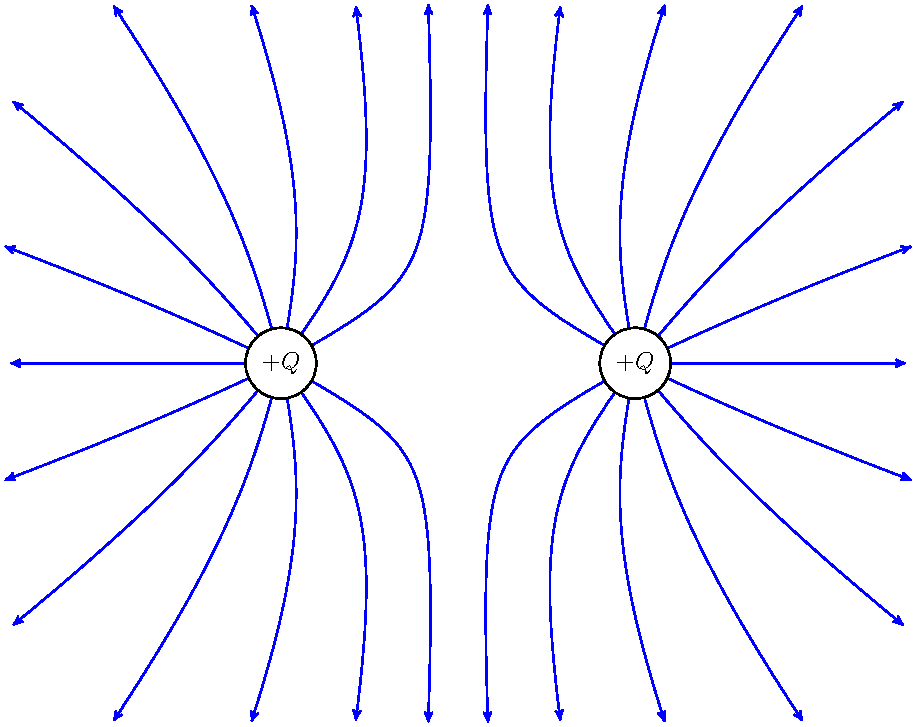
\includegraphics[width=7.2cm]{f-lines-eq-ch.pdf}
			\begin{equation*}
			\text{two positive charges}
			\end{equation*}
		\end{center}
	\end{minipage}\hfill
	\begin{minipage}{0.48\textwidth}
		\begin{center}
			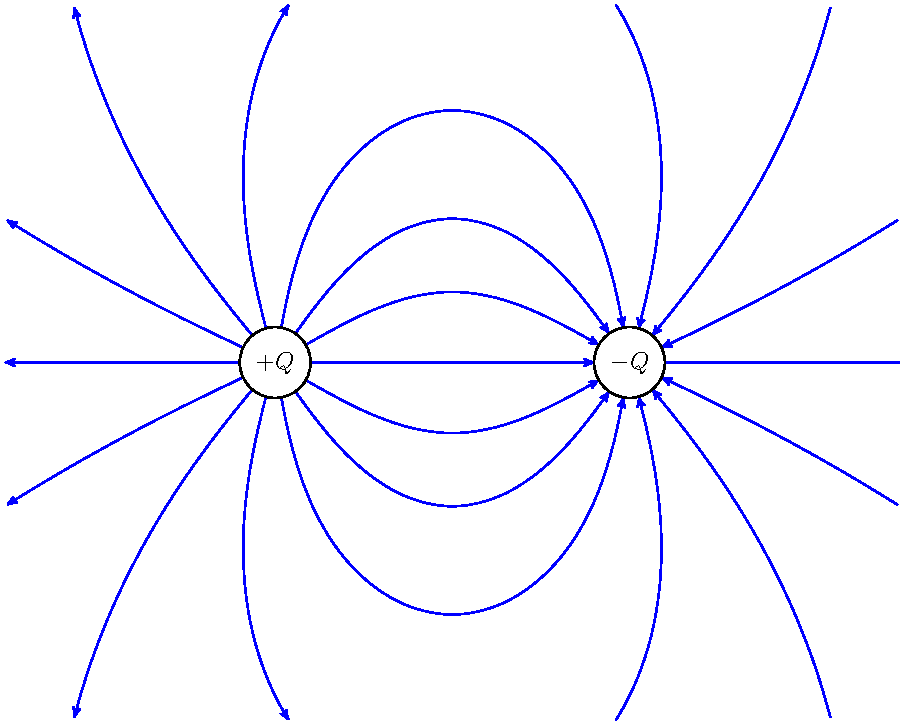
\includegraphics[width=7.2cm]{f-lines-op-ch.pdf}
			\begin{equation*}
			\text{two opposite charges} \teoe
			\end{equation*}
		\end{center}	
	\end{minipage}
\end{center}




\subsection{potential \& potential energy }

\subsubsection{electric potential energy}
\label{sec:electric-potential}

gain/loss in \keypoint{electric potential energy}\index{electric field!electric potential energy} is defined as work done against/by electric force

(compare everything in this section with what you have learned about gravitational P.E.!)

let's start to derive the electrical P.E. between two charges $Q$ and $q$ separated by $r$

again we define $E_p=0$ at $r=\infty$ (choice of zero potential energy, no force so no P.E.), then

\begin{ilight}
	\keypoint{electric potential energy} is equal to the work done by electric force to bring a charge to a specific position from \emph{infinity}
\end{ilight} 

moving a test charge $q$ from $r=\infty$ to a distance of $r$ from $Q$

\begin{center}
\begin{tikzpicture}[scale=0.8]
\draw [fill] (-4,0) circle [radius=0.1];
\node[below] at (-4,-0.1) {$Q$};
\draw [fill] (8,0) circle [radius=0.1];
\node[below] at (8,-0.1) {$q$};
\draw [thick, <->] (0,-1.2) --(-4,-1.2) node[above,midway]{$r$};
\draw [thick,dashed,gray,->] (7.7,0) -- (0.3,0) node[above,midway]{\textcolor{black}{$W$}};
\draw [fill] (0,0) circle [radius=0.1];
\draw (8,-1) node{$\infty$};
\end{tikzpicture}
\end{center}

work done by electric force: $W=\int^r_\infty F dr = \int^r_\infty \frac{Qq}{\ec} \frac{\dd x}{x^2} = - \frac{Qq}{\ec x}\bigg|^r_\infty = - \frac{Qq}{\ec r} $

\eqyskip

since $\Delta E_p=-W$, we find: $E_p(r) - E_p(_\infty) = \frac{Qq}{\ec r}$

but $E_p(_\infty) = 0$,  so electric P.E. between two charges $Q$ and $q$ is $\boxed{E_p(r) = \frac{Qq}{\ec r}}$

\cmt as $r \to \infty$, $E_p \to 0$, this agrees with our definition for zero P.E. point

\cmt for like charges, $Qq > 0$, so $E_p > 0$

to bring like charges closer, work must be done to overcome their \emph{repulsion}, P.E. increases

minimum P.E. $E_p(\infty)=0$ at infinity, so positive P.E. at finite $r$

\cmt for opposite charges, $Qq < 0$, so $E_p < 0$

to pull opposite charges apart, work must be done to overcome their \emph{attraction}, P.E. increases

maximum P.E. $E_p(\infty)=0$ at infinity, so negative P.E. at finite $r$

\cmt electric P.E. is a \emph{scalar quantity}, sign is important

repulsion implies positive P.E., and attraction implies negative P.E.

sign of P.E. is hidden in polarities of charges


\example{In $\alpha$-particle scattering experiment, we fire $\alpha$-particles ($_2^4\alpha$) towards a thin gold ($_{\phantom{0}79}^{197}\text{Au}$) foil in hope of gaining information about the nucleus. The size of a typical nucleus is about $10^{-14}$m, what is the minimum initial speed for $\alpha$-particles so that radius of gold nucleus can be determined?}
	
\sol as $\alpha$-particle approaches the nucleus, it slows down due to the repulsive interaction

kinetic energy decreases and electric potential energy increases

if it gets close enough to the nucleus before coming to a stop, nuclear radius can be estimated

{

\centering

$\text{K.E. loss} = \text{P.E. gain} \RA \frac{1}{2}mu^2 - \underbrace{\frac{1}{2}mv^2}_0 = E_p(r) - \underbrace{E_p(\infty)}_0 \RA  \frac{1}{2}mu^2= \frac{Qq}{4\pi\epsilon_0r}$

}

\begin{equation*}
	\frac{1}{2}\times4\times1.66\times10^{-27}\times u^2 = \frac{79\times1.60\times10^{-19}\times2\times1.60\times10^{-19}}{4\pi\times8.85\times10^{-12}\times10^{-14}} \RA
	u\approx 3.3\times10^7\mps \teoe
\end{equation*}

\question{A metal sphere of radius 20 cm carries a charge of $5.0\times10^{-7}$ C. A proton is sent towards the sphere at a speed of $1.8\times10^6 \mps$. Can the proton reach the surface of the sphere?}



\subsubsection{electric potential}

it is also useful to define the \emph{electric potential} for any specific point in a field

electric potential can be thought as the electric potential energy per unit charge: $V = \frac{E_p}{q}$

\begin{ilight}
	\keypoint{electric potential}\index{electric field!electric potential} is the work needed to bring a unit positive charge from infinity
\end{ilight}

\cmt unit: $[V] = \text{ J C}^{-1} = \text{V}$

\cmt electric potential due to an isolated source $Q$: $V = \frac{E_p}{q} = \frac{\frac{Qq}{\ec r}}{q} \RA \boxed{V = \frac{Q}{4\pi\epsilon_0 r}}$

\cmt potential at infinity vanishes: $V_\infty = 0$

\cmt electric potential can take both signs

the sign depends on whether unit positive charge is repelled or attracted by the source

for positively-charged sources $V>0$, while for negatively-charged sources $V<0$

\cmt electric potential is a \emph{scalar} quantity

to find combined potential due to multiple charges, add up contributions of each charge

\example{An electron is accelerated from rest through a potential difference of 600 V.
	
Find the final speed of the electron.}

\sol gain in K.E. = change in electric P.E. $\RA \frac{1}{2}mv^2 = q\Delta V$
\eqyskip\begin{equation*}
	v = \sqrt{\frac{2q\Delta V}{m}} = \sqrt{\frac{2\time 1.60\times10^{-19}\times600}{9.11\times10^{-31}}} \approx 1.45\times10^7 \mps \teoe
\end{equation*}

\example{Two small metal spheres $A$ and $B$ are in a vacuum. Sphere $A$ has charge $+20$ pC and sphere $B$ has charge $+84$ pC. The arrangement is shown below.}

\begin{figure}[ht]
	\centering
	\begin{tikzpicture}
		\draw[thick] (-5,0) circle(0.8) node[above]{$A$} (5,0) circle(0.8) node[above]{$B$};
		\draw[thick,dashed] (-5,-2.1) -- (-5,0) -- (5,0) -- (5,-2.1) (-2,0) node[above]{$P$} -- (-2,-1.5)
		(0,0) node[above]{$M$} -- (0,-1.5);
		\draw[fill] (-2,0) circle(0.05);
		\draw[fill] (0,0) circle(0.05);
		\draw[<->] (-5,-2.0) -- (5,-2.0) node[midway,above]{$10$ cm};
		\draw[<->] (-5,-1.2) -- (-2,-1.2) node[midway,above]{$3.0$ cm};
		\draw[<->] (0,-1.2) -- (-2,-1.2) node[midway,above]{$2.0$ cm};
	\end{tikzpicture}
\end{figure}

(a) Find the electric potential at point $P$ and point $M$ respectively.

(b) Find the work done to move an $\alpha$-particle from $P$ to $M$.

\sol combined electric potential: $V = V_A + V_B = \frac{1}{\ec}\left(\frac{Q_A}{r_A} + \frac{Q_B}{r_B} \right)$

\eqyskip

at $P$: $V_P = 8.99\times10^9 \times \left( \frac{+20 \times 10^{-12}}{0.030} + \frac{+84 \times 10^{-12}}{0.070} \right) \approx 16.8 \text{ V}$

\eqyskip

at $M$: $V_M = 8.99\times10^9 \times \left( \frac{+20 \times 10^{-12}}{0.050} + \frac{+84 \times 10^{-12}}{0.050} \right) \approx 18.7 \text{ V}$

from $P$ to $M$: $W = \Delta E_p = q\Delta V = q(V_M- V_P) = 2\times1.60\times10^{-19}\times(18.7-16.8) \approx 6.2\times10^{-19} \text{ J}$ \eoe

\example{$A$ and $B$ are two positively-charged spheres of radius 1.0 cm. A proton $P$ initially at rest on the surface of $A$ moves along the line joining the centres of the two spheres. The variation with distance $x$ from the centre of $A$ of electric potential $V$ at point $P$ is given.}\label{ex-V-of-two-pcs}

\begin{figure}[ht]
	\centering
	\begin{tikzpicture}[scale=1.2]
		\draw[style=help lines,step=0.2,gray!50] (0,-0) grid (6,5);
		\draw[step=1] (0,0) grid (6,5);
		\draw [very thick, color=blue, domain=0.5:5.5, smooth, samples=60, variable=\x] plot (\x,{2.2/\x + 1.1/(6-\x)});
		\draw[very thick,blue] (0,4.6) --++ (0.5,0) node[above]{$A$};
		\draw[very thick,blue] (5.5,2.6) node[above]{$B$} --++ (0.5,0);
		\foreach \x in {0,100,200,300,400,500} \node[left] at (0,\x/100) {$\x$};
		\foreach \x in {0,2,4,6,8,10,12} \node[below] at (\x/2,0) {$\x$};
		\node at (-1.35,2.5) {$V/\text{V}$};
		\node at (3,-0.8) {$x/\text{cm}$};
	\end{tikzpicture}
\end{figure}

\rcyskip (a) Find the maximum speed as the proton moves from $A$ to $B$.

(b) Find the speed when the proton reaches surface of $B$.

\sol increase in K.E. = loss in P.E., so: $\frac{1}{2}mv^2 - 0 = q\Delta V \RA \frac{1}{2}mv^2 = q(V_A - V_P)$

maximum speed when $\Delta V$ is maximum, or $V_P = 107 \text{ V}$ becomes minimum (at $x = 7.2$ cm)
\begin{equation*}
	\frac{1}{2}\times1.67\times10^{-27}\times v^2_\tmax = 1.60\times10^{-19} \times (460-107) \RA v_\tmax \approx 2.60\times10^5 \mps
\end{equation*}

at surface of $B$, $V_P = 260 \text{ V}$ (at $x=11.0$ cm)
\begin{equation*}
\frac{1}{2}\times1.67\times10^{-27}\times v^2_B = 1.60\times10^{-19} \times (460-260) \RA v_B \approx 1.96\times10^5 \mps \teoe
\end{equation*}

\question{Electrical breakdown occurs when electric field strength at surface of a metal sphere exceeds $5.0 \times 10^6 \NpC$. Given that the radius of the sphere is 16 cm. What is the electric potential at the surface when electrical breakdown occurs?}

\question{Two charged particles $A$ and $B$ are separated by 20 cm. $P$ is a point on the line $AB$. Given that particle $A$ carries charge $+7.2 \text{ }\mu\text{C}$, and electric potential is zero where $AP = 5.0$ cm. Find the electric charge of $B$.}

\question{A particle with specific charge (ratio of its electric charge to its mass) $+9.58\times10^7 \text{ C kg}^{-1}$ is moving towards a fixed metal sphere. The sphere has a potential of $+500$ V. The initial speed of the particle is $3.0\times10^5 \mps$ when it is a large distance from the sphere. Determine whether the particle can reach the surface of the sphere.}


\subsubsection{equipotential lines}

to show potential distributions, we draw \keypoint{equipotential lines}\index{equipotential lines}
\footnote{In three dimensions, these lines form equipotential \emph{surfaces}.}

points on same equipotential line have constant electric potential

i.e., equipotential lines are \emph{contour lines} of equal electric potential

\cmt for a field near a point charge, equipotential lines are a set of \emph{concentric} circles

\begin{center}
	\begin{tikzpicture}[scale=1]
	\draw (-3,0) node{$+Q$} circle [radius=0.5];
	\foreach \s in {0,45,90,...,315}
	\draw [blue, thick, ->] (-3,0) ++ (\s:0.5) -- ++(\s:1.8);
	
	\draw (3,0) node{$-Q$} circle [radius=0.5];
	\foreach \s in {0,45,90,...,315}
	\draw [blue, thick, <-] (3,0) ++ (\s:0.5) -- ++(\s:1.8);
	
	\foreach \s in {0.9,1.4,1.9}{
		\draw [red,dashed] (-3,0) circle(\s) (3,0) circle(\s);}
	\end{tikzpicture}
\end{center}

\cmt for uniform fields, equipotential lines are a set of \emph{parallel} straight lines

\begin{center}
	\begin{tikzpicture}[yscale=1.2]
	\draw (-5,1.2) rectangle (5,1.6);
	\draw (-5,-1.2) rectangle (5,-1.6);
	\foreach \charge in {-4.5,-3.5,...,4.5}{
		\draw (\charge,1.4) node {$+$} (\charge,-1.4) node {$-$};
		\draw[thick,blue,->] (\charge,1.2) --++ (0,-2.4);	
	}
	\foreach \s in {-0.8,0,0.8} \draw[red,dashed] (-5,\s) -- (5,\s);
	\end{tikzpicture}
\end{center}
	

	
\cmt equipotential lines are always perpendicular to the electric field lines
	
moving along an equipotential line requires no work done

\example{Field lines and equipotential lines due to two charges of various magnitudes}

\begin{center}
	\noindent\begin{minipage}{0.48\textwidth}
		\begin{center}
			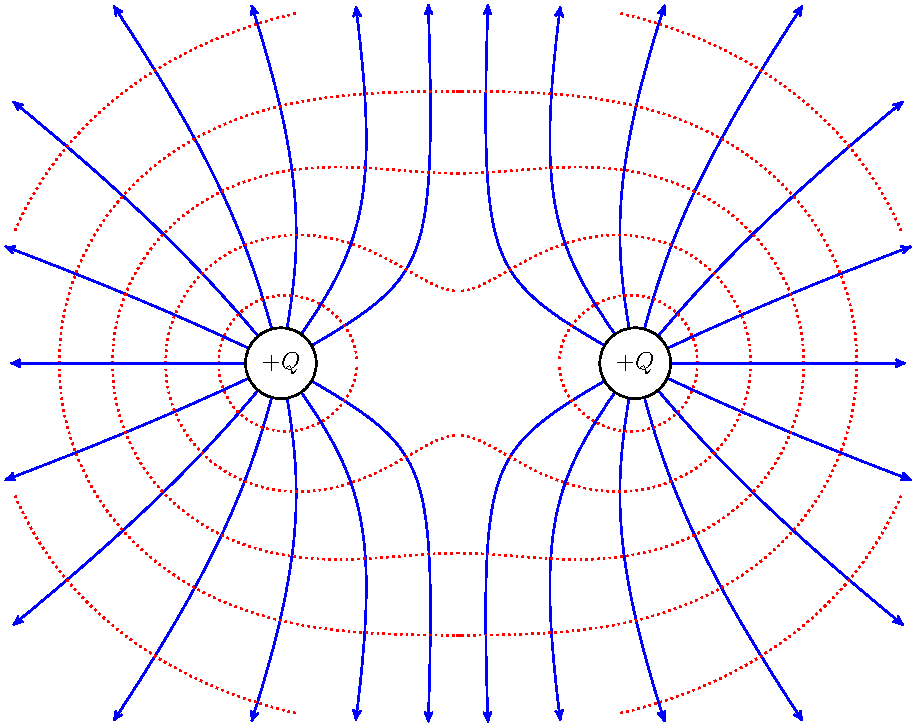
\includegraphics[width=7cm]{f-all-eq-ch.pdf}
		\end{center}
	\end{minipage}\hfill
	\begin{minipage}{0.48\textwidth}
		\begin{center}
			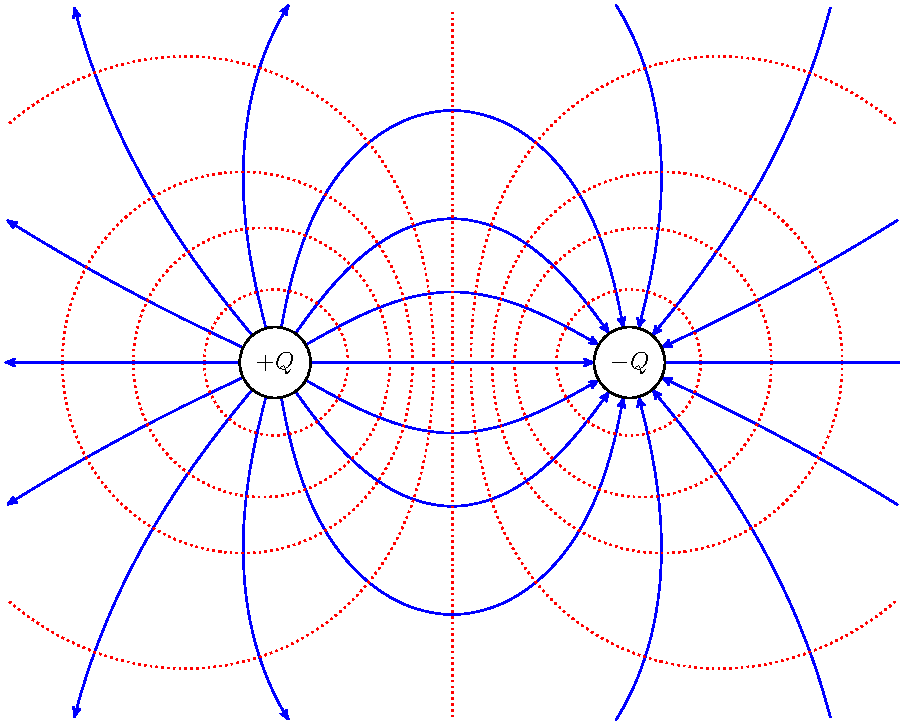
\includegraphics[width=7cm]{f-all-op-ch.pdf}
		\end{center}
	\end{minipage}
\end{center}

\begin{center}	
	\noindent\begin{minipage}{0.48\textwidth}
		\begin{center}	
			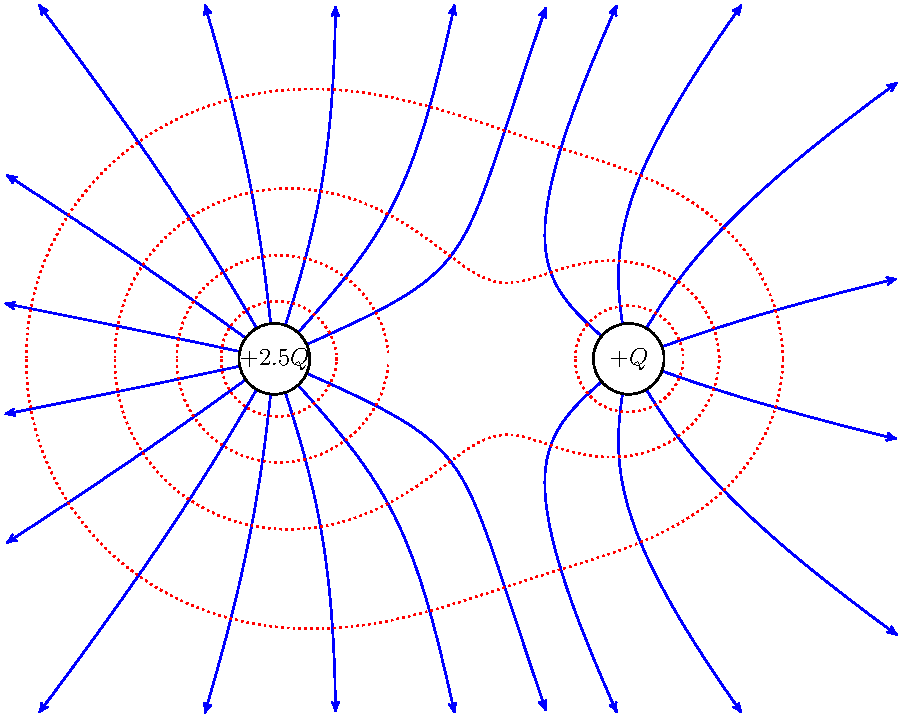
\includegraphics[width=7cm]{Q2p.pdf}
			\end{center}
		\end{minipage}\hfill
	\begin{minipage}{0.48\textwidth}
		\begin{center}
			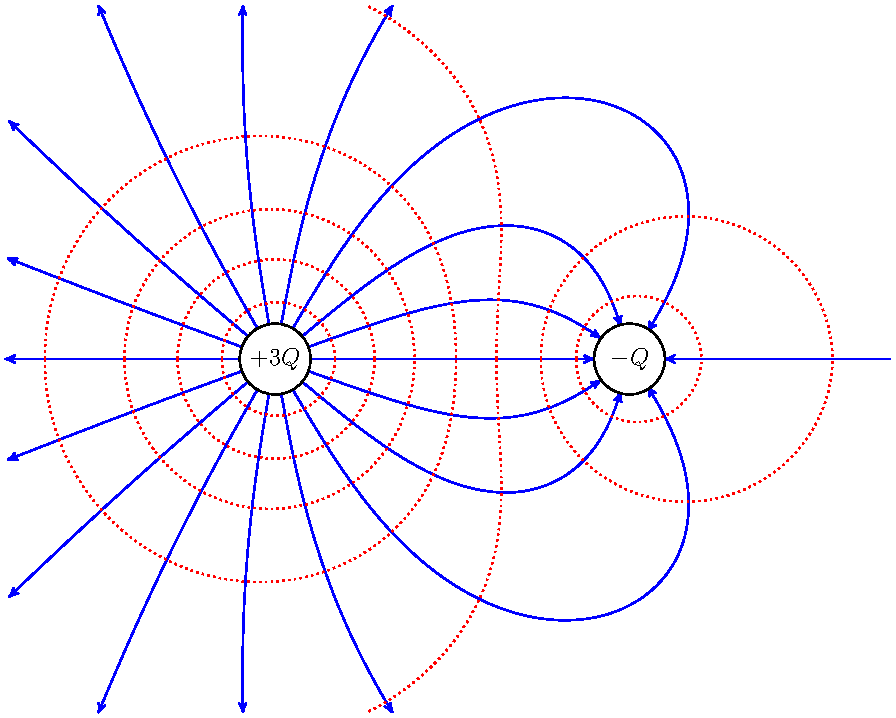
\includegraphics[width=7cm]{Q4n.pdf}
		\end{center}
	\end{minipage}
\end{center}

\begin{center}	
	\noindent\begin{minipage}{0.48\textwidth}	
		\begin{center}	
			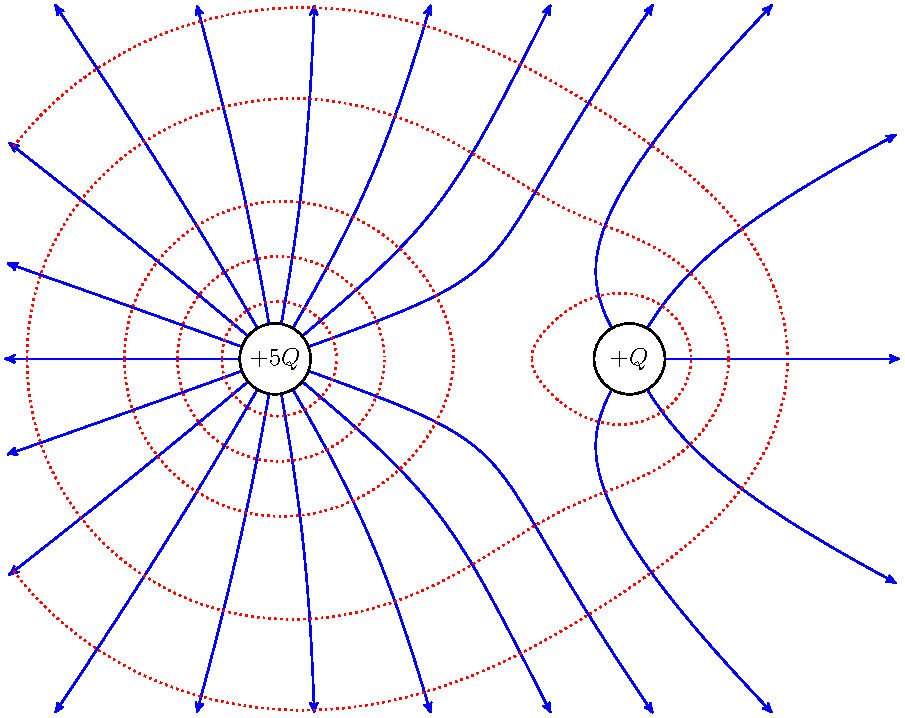
\includegraphics[width=7cm]{Q5p.pdf}
		\end{center}
	\end{minipage}\hfill
	\begin{minipage}{0.48\textwidth}
		\begin{center}
			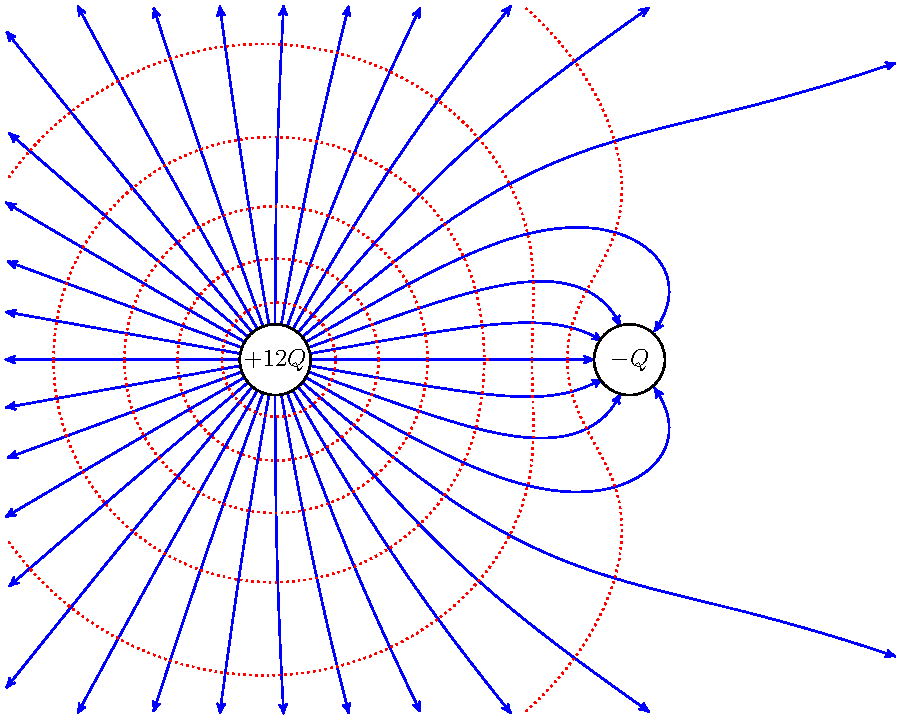
\includegraphics[width=7cm]{Q12n.pdf}
		\end{center}	
	\end{minipage}
\end{center}



\subsection{further discussions on electric fields}

\subsubsection{comparison with gravitational fields}

both gravitational and electric force are described by inverse square law, so it follows that the mathematical language for both theories are very similar

\cmt physical quantities that describe gravitational/electric fields

\begin{center}
	\begin{tabular}{|c|c|c|}
		\hline
		& vector description & scalar description \\ \hline 
		interaction between two masses/charges & force $F$ & potential energy $E_p$ \\ \hline
		effect of source mass/charge & field $g$/$E$ & potential $\varphi$/$V$ \\ \hline
	\end{tabular}
\end{center}

\cmt comparing gravitational field with electric field
\footnote{Note that there is no negative mass, gravitational force always interacts attractively. This is the fundamental difference between gravitational fields and electric fields.}

\begin{center}
{\renewcommand{\arraystretch}{1.28}
\begin{tabular}{|c|c|c|c|}
\hline
& gravitational field & electric field & meaning \\ \hline 
force & $F=(-)G \frac{Mm}{r^2}$ & $F=\frac{1}{4\pi\epsilon_0} \frac{Qq}{r^2}$ & force between masses/charges\\ [1ex] \hline
field strength & $g= \frac{F}{m} = (-)G \frac{M}{r^2}$ & $E= \frac{F}{q} = \frac{1}{4\pi\epsilon_0} \frac{Q}{r^2}$ & force per unit mass/charge\\ [1ex] \hline
potential energy &  $E_p = -G \frac{Mm}{r}$ & $E_p=\frac{1}{4\pi\epsilon_0} \frac{Qq}{r}$ & related to work done by force \\ [1ex] \hline
potential & $\varphi = \frac{E_p}{m} = -G \frac{M}{r}$ & $V = \frac{E_p}{q} = \frac{1}{4\pi\epsilon_0} \frac{Q}{r}$ & energy per unit mass/charge\\ [1ex] \hline
\end{tabular}}
\end{center}

\cmt similarities between gravitational field and electric field

\begin{itemize}
	\item[-] force and field strength both obey \emph{inverse square laws}
	
	\item[-] potential energy and potential is inversely proportional to separation
	
	\item[-] no potential energy and no potential at infinite separation
\end{itemize}

\cmt differences between gravitational field and electric field

mass (source of gravity) is always positive, but electric charges can be positive or negative

this fact leads to many fundamental differences between the two force fields

\begin{itemize}
\item[-] electric force can be repulsive or attractive, but gravitational force is always attractive

\item[-] electric potential can take both signs, but gravitational potential is always negative
\end{itemize}

\subsubsection{electric field inside conductors}\label{inside-conductors}

consider electric field \emph{inside} a metal conductor carrying charge $Q$

conductor means there are free charge carriers that can move around 

but charge distribution should be stable for a charged conductor (no circulating currents)

so charge carriers must experience no force, i.e., field strength inside conductor is zero

put it the other way round, if there is an excess field, it will push free charge carriers to move around, until they are distributed so that the field inside the conductor becomes zero

moreover, there shall be no potential difference between any two points inside the conductor, otherwise charge carriers would flow, so electric potential must be constant

\begin{ilight}
	\centering
	
	electric field strength is everywhere zero inside a conductor: $E=0$
	
	electric potential is everywhere constant inside a conductor: $V=\text{const}$
\end{ilight}

\example{Consider the electric field due to a metal sphere of radius $R$ carrying charge $Q$. Plot the variation with the distance $r$ from sphere's centre of the field strength, and the variation with $r$ of the electric potential.}\label{ex-metal-sphere}


\sol charge $Q$ is uniformly spread out on \emph{surface} of sphere

viewed from \emph{outside}, the sphere appears to have all of its charge concentrated at the centre

so it can be modelled as a point charge due to its symmetric distribution of charges

electric field strength at distance $r$ from sphere's centre is: $E = \frac{Q}{\ec r^2}$ for $r>R$

electric potential at distance $r$ from sphere's centre is: $V=\frac{Q}{4\pi\epsilon_0r}$ for $r>R$

\emph{inside} the sphere, i.e., for $r<R$, we have $E=0$, and $V=\frac{Q}{\ec R} = \text{const}$ \eoe

\begin{figure}[ht]
	\centering
	\noindent\begin{minipage}{0.45\linewidth}
		\centering
		\begin{tikzpicture}[yscale=1.2,xscale=1.2]
		\draw[thick,<->] (0,5) node[left]{$E$} -- (0,0) -- (1,0) node[below]{$R$} -- (4.5,0) node[below]{$r$};
		\draw [thick,color=blue,domain=1:4.5,samples=20,smooth,variable=\x] plot (\x,{4.5/\x/\x});
		\draw[thick,blue] (0,0.02) -- (1,0.02);
		\draw[dashed] (0,4.5) node[left]{$E_0$} -- (1,4.5) -- (1,0) node[below]{$R$};
		\draw[dashed] (0,4.5/4) node[left]{{\scriptsize $\frac{E_0}{4}$}} -- (2,4.5/4) -- (2,0) node[below]{$2R$};
		\draw[dashed] (0,4.5/9) node[left]{{\scriptsize $\frac{E_0}{9}$}} -- (3,4.5/9) -- (3,0) node[below]{$3R$};
		\end{tikzpicture}
		

	\end{minipage}
	\begin{minipage}{0.45\linewidth}
		\centering
		\begin{tikzpicture}[yscale=1.2,xscale=1.2]
		\draw[thick,<->] (0,5) node[left]{$V$} -- (0,0) -- (1,0) node[below]{$R$} -- (4.5,0) node[below]{$r$};
		\draw [thick,color=blue,domain=1:4.5,samples=20,smooth,variable=\x] plot (\x,{4.5/\x});
		\draw[dashed] (0,4.5) node[left]{$V_0$} -- (1,4.5) -- (1,0) node[below]{$R$};
		\draw[dashed] (0,4.5/2) node[left]{{\scriptsize $\frac{V_0}{2}$}} -- (2,4.5/2) -- (2,0) node[below]{$2R$};
		\draw[dashed] (0,4.5/3) node[left]{{\scriptsize $\frac{V_0}{3}$}} -- (3,4.5/3) -- (3,0) node[below]{$3R$};
		\draw[thick,blue] (0,4.5) -- (1,4.5);
		\end{tikzpicture}
		

	\end{minipage}
\captionsetup{labelformat=empty}

\caption{Example \ref{ex-metal-sphere}: field strength and potential due to a charged metal sphere}
\end{figure}


\question{State whether the two spheres in Example \ref{ex-V-of-two-pcs} are conductors. State what feature of the potential graph supports your answer.}

\question{You might have the experience that your mobile phone signal gets much weaker when you get into an elevator. Explain why this happens.}

\subsubsection{field strength \& potential}\label{field-strength-potential}

for a small displacement $\Delta r$ in an electric field, change in potential $\Delta V$ is

{

\centering

$\Delta V = \frac{\Delta E_p}{q} \xlongequal{\Delta E_p=-W} - \frac{\Delta W}{q} = - \frac{F \Delta r}{q} \xlongequal{F=Eq} - E \Delta r \RA E = - \frac{\Delta V}{\Delta r}$

}

\eqyskip as change in displacement $\Delta r \to 0$, we have $\boxed{E = - \frac{\dd V}{\dd r}}$

therefore we have the following theorem:

\begin{ilight}
	\centering field strength is negative gradient of potential with respect to displacement
\end{ilight}

can also consider change in potential $\Delta V$ for large distance due to work done in a field

{
	
\centering

$\Delta V= \int \dd V \xlongequal{E = -\dd V/\dd r}  \int (-)E \dd r =  -\int E \dd r$
\footnote{The expression is implicitly integrated from initial position to final position.}

}

\eqyskip this gives the inverse relation: $\boxed{\Delta V = -\int E \dd r}$
\footnote{These equations are correct if the charge is moving in the parallel direction to the field, i.e., the motion is along the field lines. But an object can move in all directions in the field. More rigorously, if we take the vector nature of electric field into account, we should write $\Delta V = - \int \mathbf{E}\cdot\dd\mathbf{r}$, and $\mathbf{E} = - \frac{\partial V}{\partial \mathbf{r}}$. ($\star$)}

\cmt given a $V$-$r$ graph, gradient of curve gives field strength

conversely, given a $E$-$r$ graph, area under curve gives change in potential

\cmt can also write $F = - \frac{\dd U}{\dd r}$ and $\Delta U = -\int F \dd r$

force always acts in a direction to lower the potential energy of an object
\footnote{This result can be generalised to a very important principle of physical laws called the \emph{least action principle}. It states that any motion of a system tends to minimise the action, a physical quantity related to the energy of the system. This fundamental law plays a crucial role in the study of theoretical physics. ($\star$)}

\example{The variation of electric potential near a charged object is shown on the graph. Calculate the electric field strength at 5.0 cm from the centre of the object.}\label{ex-grad-pot}

\begin{figure}[ht]
	\centering
	\begin{tikzpicture}[scale=0.54]
	\draw[style=help lines,step=0.5,gray!30] (0,0) grid (12,12);
	\draw[style=help lines,step=2] (0,0) grid (12,12);
	\draw [thick] (12,0) node[below]{$r/\text{cm}$};
	\draw [thick] (0,12) node[left]{$V/\text{kV}$};
	\foreach \s in {0,2,...,10}
	{
		\draw (\s,0) node[below]{\s};
		\draw (0,\s) node[left]{\s};
	}
	\draw[very thick,purple,domain=2:10,samples=15,smooth,variable=\x] plot (\x,20/\x);
	\draw[thick,red,domain=1:9,samples=2,smooth,variable=\x] plot (\x,-0.8*\x+8);
	\draw[fill] (5,4) circle[radius=0.15];
	\draw[thick,blue] (2,6.5) -- (2,1.5) -- (8,1.5);
	\end{tikzpicture}
\end{figure}

\sol draw tangent to the graph at $r=5.0\text{ cm}$ (red line), gradient of tangent gives field strength:

$ \text{gradient} = \frac{\Delta V}{\Delta r} = \frac{(1.5-6.5)\times 10^3}{(8.0-2.0)\times10^{-2}} \approx  -8.3\times10^4 \Vpm \RA E = -\frac{\Delta V}{\Delta r} = 8.3\times10^4 \Vpm $ \eoe 

\question{Show that the charged object in Example \ref{ex-grad-pot} behaves like a point charge. Determine the charge it carries, and hence calculate the field strength at $r=5.0$ cm.}

\example{The variation of electrical potential along a certain line is shown. State and explain where in the field an electron will experience the greatest force.}

\begin{figure}[ht]
	\centering
	\begin{tikzpicture}[scale=1.2]
	\draw[style=help lines,step=0.25,gray!30] (0,-2) grid (8,4);
	\draw[style=help lines,step=1] (0,-2) grid (8,4);
	\node[left] at (0,4) {$V$};
	\node[left] at (0,0) {0};
	\foreach \x in {0,1,...,8} {
		\draw[white,fill] (\x-0.1,-0.32) rectangle (\x+0.1,-0.08);
		\node[below] at (\x,0) {$\x$};
	}
	\draw[thick, purple, domain=1:7, samples=25, smooth, variable=\x] plot (\x,{4/\x/\x-2/(8-\x)/(8-\x)});
	\node[right] at (8.1,0) {$x/\text{cm}$};
	\end{tikzpicture}
\end{figure}

\sol greatest force means greatest field strength, which means maximum potential gradient 

largest gradient of $V$-$x$ curve at $x=1$ cm, so greatest force at $x=1$ cm \eoe

\example{electric field due to an isolated point charge}

we have learned that the electric potential due to a point charge is: $V = \frac{Q}{\ec r}$
	
using $E = -\frac{\dd V}{\dd r}$, we have $E = -\frac{\dd}{\dd r}\left( \frac{Q}{4\pi\epsilon_0r} \right) = -\frac{Q}{4\pi\epsilon_0}\frac{\dd}{\dd r}\left(\frac{1}{r}\right) = \frac{Q}{4\pi\epsilon_0r^2}$

this agrees with the expression for field strength due to an isolated charge \eoe

\question{For the electric field due to a charged metal sphere (see Example \ref{ex-metal-sphere}), convince yourself that the field strength equals negative gradient of potential at any point.}

\question{We have seen the statement field strength equals negative potential gradient holds for electric fields. Does it also hold for gravitational fields?}




\subsubsection*{uniform fields revisited}

given two oppositely-charged metal plates separated by a distance of $d$

if p.d. between the plates is $V$, then electric field strength between is given by $E = \frac{V}{d}$\footnote{You should have learned this in AS-level physics.}

we will derive this result using the theorem introduced in the last section

\begin{figure}[ht]
\centering
\begin{minipage}{0.48\textwidth}
	\centering
	\begin{tikzpicture}[scale=0.8]
	\foreach \s in {1,2,3,4}
	\draw[thick,blue,<-] (0,\s) -- (5,\s);
	\draw (2.5,4) node[above]{$E$};
	\draw [thick,gray,dashed,<-] (1,2.5) -- (4,2.5);
	\shade [ball color = green] (4,2.5) circle [radius=0.1] node[right]{$q$};
	\draw [thick] (5,0.5) -- (5,4.5) node[above]{$+$};
	\draw [thick] (0,0.5) -- (0,4.5) node[above]{$-$};
	\draw[<->] (0,0) -- (5,0) node[midway, above] {$d$};
	\end{tikzpicture}
\end{minipage}\hfil
\begin{minipage}{0.48\textwidth}
	\centering
	\begin{tikzpicture}[scale=0.8]
		\draw [thick,<->] (0,4.2) node[left]{$V$} -- (0,0) -- (5.6,0) node[below]{$r$};
		\draw[dashed] (5,3.6) -- (5,0) node[below]{$d$}; 
		\draw [very thick,red] (0,0) -- (5,3.6);
	\end{tikzpicture}
\end{minipage}
\captionsetup{labelformat=empty}

\caption{moving a test charge in a uniform electric field}
\end{figure}


moving a test charge $q$ in a uniform field, work done by electric force: $W=Fd = Eqd$
		
change in P.E.: $\Delta E_p = -W = -Eqd$

change in potential: $\Delta V = \frac{\Delta E_p}{q} = - Ed$, or $E=-\frac{\Delta V}{d}$

plotting $V$-$r$ graph, $\text{gradient of line}=-E$

the minus sign means field strength points in the direction such that potential decreases

i.e., electric field acts from high potential to low potential



\subsubsection*{electric field due to two positive point charges}

two point charges $+Q_1$, $+Q_2$ are separated by a distance of $D$

let's look into the electric field along the segment joining the two charges 

\begin{center}
\begin{tikzpicture}[scale=0.8]
\shade [ball color = green] (-4,0) node[above]{$+Q_1$} circle (0.15);
\shade [ball color = green] (4,0) node[above]{$+Q_2$} circle (0.15);
\draw [thick, <->] (-4,-2)--(4,-2) node[midway,above]{$D$} ;
\draw [thick, <->] (-4,-1)--(-1,-1) node[midway,above]{$r_1=x$};
\draw [thick, <->] (-1,-1)--(4,-1) node[midway,above]{$r_2=D-x$};
\draw [thick, <->] (-4,-2)--(4,-2) node[midway,above]{$D$} ;
\draw [dashed] (-4,-0.5) -- (-4,-2.2);
\draw [dashed] (4,-0.5) -- (4,-2.2);
\draw [dashed] (-1,-0.5) -- (-1,-1.5);
\draw [->,thick,blue] (-1,0) -- ++(-0.9,0) node[above]{$E_2$};
\draw [->,thick,blue] (-1,0) -- ++(2.5,0) node[above]{$E_1$};
\draw [fill] (-1,0) node[above]{$q$} circle [radius=0.1];
\end{tikzpicture}
\end{center}

combined potential: $V = V_1 + V_2 = \frac{Q_1}{4\pi\epsilon_0r_1} + \frac{Q_2}{4\pi\epsilon_0r_2} = \frac{1}{4\pi\epsilon_0}\left(\frac{Q_1}{x} + \frac{Q_2}{D-x}\right)$

combined field strength: $E = E_1 - E_2 = \frac{Q_1}{4\pi\epsilon_0r_1^2} - \frac{Q_2}{4\pi\epsilon_0r_2^2} = \frac{1}{4\pi\epsilon_0}\left(\frac{Q_1}{x^2} - \frac{Q_2}{(D-x)^2}\right)$

notice that when computing $V$, we carry out \emph{scalar sum}

but for $E$, we carry out \emph{vector sum}, i.e., directions of $E_1$ and $E_2$ become important

$V$-$x$ graph and $E$-$x$ graph for the case where $Q_1=3Q_2$ are sketched

\begin{center}
	\begin{tikzpicture}[scale=1.35]
	\draw[thick,->] (0,-2) -- (0,4.8);
	\draw[thick,->] (0,0) -- (9,0) node[below]{$x$};
	\draw [thick,color=blue,domain=0.3:7.7,samples=60,smooth,variable=\x] plot (\x,{(.24/\x/\x-.08/(8-\x)/(8-\x))*1.5}) node[below]{$E$};
	\draw [thick,color=red,domain=0.3:7.7,samples=60,smooth,variable=\x] plot (\x,{(.3*3/\x+.1*3/(8-\x))*1.5}) node[above]{$V$};
	\draw[dashed] (8,-2) -- (8,3);
	\shade [ball color = green] (0,0) node[below right]{$+Q_1$} circle (0.15);
	\shade [ball color = green] (8,0) node[below right]{$+Q_2$} circle (0.15);
	\end{tikzpicture}
\end{center}

\question{Convince yourself that field strength is indeed given by negative potential gradient. You may interpret it either graphically (think about gradient of tangent along the curve) or algebraically (think about the derivative of $V$).}

\question{We have looked into the electric field between two positively-charged particles. Discuss the cases where (a) both particles are negatively charged, (b) the two particles carry opposite charges.}
\section{Capacitors}

\subsection{capacitors: an introduction}

\subsubsection{capacitors}

\begin{wrapfigure}{r}{6cm}
\centering
\begin{tikzpicture}[scale=0.5]
\coordinate (A1) at (0,0); 
\coordinate (A2) at (0.5,0);
\coordinate (A3) at (2.5,0); 
\coordinate (A4) at (3,0);
\coordinate (B1) at (0,4); 
\coordinate (B2) at (0.5,4);
\coordinate (B3) at (2.5,4); 
\coordinate (B4) at (3,4);
\coordinate (C1) at (1.2,5.5); 
\coordinate (C2) at (1.7,5.5);
\coordinate (C3) at (3.7,5.5); 
\coordinate (C4) at (4.2,5.5);
\coordinate (D4) at (4.2,1.5);
\draw [thick,fill=gray!50] (A1) -- (A2) -- (B2) -- (C2) -- (C1) -- (B1) -- cycle;
\draw [thick,fill=cyan!20] (A2) -- (A3) -- (B3) -- (C3) -- (C2) -- (B2) -- cycle;
\draw [thick,fill=gray!50] (A3) -- (A4) -- (B4) -- (C4) -- (C3) -- (B3) -- cycle;
\draw [thick,fill=gray!50] (A4) -- (B4) -- (C4) -- (D4) -- cycle;
\draw [thick] (B1) -- (B4);
\draw [ultra thick] (3.6,2.7) [out=0, in=180] to (6,2) node[below]{lead};
\draw [ultra thick] (0,2.7) [out=180, in=0] to (-1.5,2) node[below]{lead};
\draw [thick] (3.6,4) -- ++ (1.5,1) node[right,align=center,execute at begin node=\setlength{\baselineskip}{1.2em}]{metal\\plate};
\draw [thick] (1.5,0.5) -- ++ (1.2,-1) node[right]{dielectric};
\end{tikzpicture}
\vspace*{-20pt}
\end{wrapfigure}

\keypoint{capacitors}\index{capacitor} are elementary electrical units widely used in electrical and electronic engineering

a typical capacitor has two conductive plates

between the plates there is usually an insulating material called \emph{dielectric}

circuit symbol for a capacitor is 
\begin{tikzpicture}[scale=0.2]
\draw (0,0) -- (1.6,0) (2.4,0) -- (4,0);
\draw (1.6,-1) -- (1.6,1) (2.4,-1) -- (2.4,1);
\end{tikzpicture}

\vspace*{\baselineskip}

\begin{wrapfigure}{r}{5.6cm}
\vspace*{-20pt}
\centering
\begin{circuitikz}[european resistors]
	\draw (2,-2) -- (-2,-2)  to[battery,l^=$\mathcal{E}$] (-2,2) -- (-0.5,2);
	\draw (2,-2) -- (2,-2)  to[R,l_=$R$] (2,2) -- (0.5,2);
	\draw (0,-2) -- (0,-1) to[C,l_=$C$] (0,1) -- (0,1.2);
	\draw[fill=white] (0.5,2) circle(0.06) node[above]{$Y$};
	\draw[fill=white] (-0.5,2) circle(0.06) node[above]{$X$};
	\draw[very thick] (0,1.2) --++ (80:1);
	\draw[fill=white] (0,1.2) circle(0.06) node[right]{$S$};
\end{circuitikz}
\end{wrapfigure}

if we construct an electric circuit as shown

when contact $S$ is moved to $X$, capacitor is connected to a voltage supply and becomes charged

positive and negative charges are separated onto two plates, and they will stay where they are even if we disconnect the capacitor from the voltage supply

if we then move $S$ to $Y$, the charged capacitor discharges and drives a current through resistor $R$, i.e., it can act as a temporary power source\footnote{Details on charging and discharging processes will be gone through in \S\ref{sec:charging-capacitors}.}

so capacitors can be used to store and release energy\footnote{Other important functions of capacitors in electronic circuits include smoothing output voltage of power supplies, blocking direct current while allowing alternating current to pass, etc.}


\subsubsection{mutual capacitance}

to describe ability of a capacitor to store charges, we define the notion of capacitance

\begin{ilight}
	\keypoint{(mutual) capacitance}\index{capacitance!mutual capacitance} of a parallel-plate capacitor is defined as the ratio of the charge stored on one plate to the potential difference across the two plates.
\end{ilight}

in a word equation: $\text{mutual capacitance } C = \frac{\text{charge on one plate }Q }{\text{p.d. } V \text{ across the plates}}$ $\quad \Rightarrow \quad$ $\boxed{C = \frac{Q}{V}}$


\cmt unit of capacitance: \keypoint{farad}\index{farad}
\footnote{The unit is named after Michael Faraday, a British physicist who developed the concept of capacitance. Faraday's other main discoveries include electromagnetic induction and electrolysis. He established the basis for the concept of the electromagnetic field in physics.}
: $[C] = \text{F}$

farad a derived unit: $1 \text{ F} = 1 \text{ C}\cdot\text{V}^{-1}$

farad is a large unit, more common subunits of capacitance in use are sub-multiples of farad:

{
	
\centering

$1 \muF = 10^{-6} \text{ F}, \quad 1 \text{ nF} = 10^{-9} \text{ F}, \quad 1 \pF = 10^{-12} \text{ F}$

}

\cmt for a parallel-plate capacitor, charges on the two plates are equal but opposite

net charge on the capacitor: $Q_\text{net} = (+Q)+(-Q)=0$

so we should emphasise on the notion of charge on \emph{one} plate in the definition



\cmt capacitance depends on \emph{geometry} of the device and permittivity of the dielectric material

capacitance does not depend on electric field or potential\footnote{Recall the resistance of an electrical component. Resistance is defined as the ratio of p.d. to current, but the value of resistance is essentially dependent on the length, cross-sectional area and material of the component, instead of the p.d. applied or the current flowing through it.}

for example, capacitance between two metal plates is: $C=\frac{\epsilon_0 A}{d}$
\footnote{If there is \emph{dielectric} in between, the formula should be rewritten as $C = \frac{\epsilon A}{d}$, where $\epsilon$ is permittivity of dielectric. These formulae are not examinable by the syllabus.}

$A$ is area of plate, $d$ is distance between plates, both are geometrical quantities



\subsubsection{self-capacitance}

there are two closely related notions of capacitance: \emph{mutual} capacitance and \emph{self} capacitance

the definition for capacitance given in the previous section, is actually \emph{mutual} capacitance\footnote{In many cases, the term capactiance is a shorthand for mutual capacitance.}

on the other hand, all bodies are able to store electrical charge

any object that can be electrically charged exhibits capacitance

we define \keypoint{self-capacitance}\index{capacitance!self-capacitance} of an object as the amount of charge that must be added to increase per unit electrical potential

in a word equation, $ \text{self capacitance }C=\frac{\text{charge of object }Q}{\text{electric potential of object }V} \RA \boxed{C=\frac{Q}{V}}$\footnote{For either mutual capacitance or self capacitance, defining equation $C=\frac{Q}{V}$ takes the same form, but you should keep in mind that $Q$ and $V$ represent different things in different contexts.}

\example{Self-capacitance of a charged metal sphere in a vacuum}

consider a metal sphere of radius $R$ and carries an electric charge of $Q$

its electric potential: $V = \frac{Q}{\ec R}$

self-capacitance of the sphere: $C_\text{sphere} = \frac{Q}{V} = Q \times \frac{\ec R}{Q} \RA \boxed{C_\text{sphere} = \ec R}$

note that capacitance is only dependent on its geometrical property (radius $R$) \eoe

\example{A conducting sphere of radius 1.0 m is situated in free space. (a) Find its capacitance. (b) In order to raise its potential to 5000 V, find the amount of charge needed.}

\sol capacitance of the sphere: $C = \ec R = 4\pi\times8.85\times10^{-12}\times 1.0 \approx 1.11\times10^{-10} \text{ F}$

(here you can see farad being an impractically huge unit)

charge on sphere: $Q = CV = 1.11\times10^{-10} \times 5000 \approx 5.56\times 10^{-7} \text{ C}$ \eoe

\subsubsection*{analogy with ideal gases}

an interesting analogy can be made between capacitors and ideal gases

recall an ideal gas is described by equation $pV=nRT$
\footnote{Don't confuse voltage $V$ with volume $V$!}

compare $\left\{\begin{array}{lccl}
\text{amount of charge:} & Q & = &CV \\ \text{amount of substance:} &n & = & \left(\frac{V}{RT}\right) p
\end{array}\right.$

\eqyskip
volume $V$ of a container has a certain space \emph{capacity}, at fixed $T$, pumping more gas (increase $n$) into system, pressure $p$ increases

similarly, a capacitor has a certain charge capacity, adding more charge $Q$ increases p.d. $V$, so the quantity $C$ is naturally called \emph{capacitance}

also for a container, there exists a maximum pressure which it can withstand

for a capacitor, there exists a \emph{breakdown voltage}, or \emph{withstand voltage}, beyond which there could be sparkling across the capacitor

\subsection{energy stored in a capacitor}

to charge a capacitor, need to push electrons off one plate and onto the other

separation of positive and negative charges requires work done $\ra$ energy is stored

\begin{wrapfigure}{l}{5.6cm}
	\vspace*{-8pt}
	\centering
	\begin{tikzpicture}[scale=1]
	\draw [gray!50, fill] (0,0) -- (3.5,2.5) -- (3.5,0) -- cycle;
	\draw [thick,<->] (0,3) node[left]{$V$} -- (0,0) -- (4,0) node[below]{$Q$};
	\draw [ultra thick, blue] (0,0) -- (3.5,2.5);
	\draw (2.5,1) -- (1.6,2) node[above,align=center,execute at begin node=\setlength{\baselineskip}{1.2em}]{energy\\stored};
	\end{tikzpicture}
	\vspace*{-16pt}
\end{wrapfigure}

since charge $Q$ varies with p.d. $V$, we shall use the $V$-$Q$ graph to find work done $W$

area under $V$-$Q$ graph is equal to work done $W$

{
	
	\centering
	
	$W = \frac{1}{2} QV$
	
}

substitute $Q=CV$, energy stored in capacitor is\footnote{Rigorously speaking, this electrical potential energy is stored within the \emph{electric fields} between metal plates of capacitor.}:

{

\centering

$\boxed{W = \frac{1}{2}CV^2 = \frac{Q^2}{2C}}$

} 

\example{When the p.d. across a capacitor of $1.8\times10^{-4} \text{ F}$ is increased from 10 V to 20 V, how much additional energy is stored?}

\sol energy change: $\Delta W = W_f - W_i = \frac{1}{2}CV_f^2 - \frac{1}{2}CV_i^2 = \frac{1}{2}\times 1.8\times10^{-4}\times(20^2-10^2) = 2.7\times10^{-2} \text{ J}$ \eoe

\question{A capacitor of 2500 $\muF$ is charged to a working voltage of 18 V. (a) What is the magnitude of positive charge on its plate? (b) What is the energy stored?}

\question{A capacitor initially charged to a potential difference of 16 V discharges and loses 40\% of its energy. What is its new p.d.?}

\question{For an isolated metal sphere of radius 30 cm situated in vacuum, what is the electric potential energy stored when charged to a potential of 120 kV?}


\newpage

\subsection{capacitor networks}

\subsubsection{capacitors in parallel}

\begin{wrapfigure}{r}{6cm}
\vspace*{-20pt}
\centering
\begin{circuitikz}[european resistors,scale=0.9]
\draw (0,0) -- (0,1.6) to[C] (3,1.6) -- (3,0) to[C] (0,0);
\node [below] at (2.1,1.6) {$C_1$};
\node [below] at (0.9,1.6) {$Q_1$};
\node [below] at (2.1,0) {$C_2$};
\node [below] at (0.9,0) {$Q_2$};
\draw (-1,0.8) -- (0,0.8) (3,0.8) -- (4,0.8);
\draw [<->] (0,2.5) -- (1.5,2.5)node[above]{$V$} -- (3,2.5);
\foreach \y  in {0,3} \draw (\y,2.3) -- (\y,2.7);
\end{circuitikz}
\end{wrapfigure}

consider two capacitors connected in parallel

same p.d. $V$ across the network: $V=V_1=V_2$

but charge $Q$ is shared: $Q_\text{total} = Q_1 + Q_2$

{

\centering

$\frac{Q_\text{total}}{V} = \frac{Q_1}{V} + \frac{Q_2}{V}$

$C_\text{total} = C_1 + C_2$

}


if three of more capacitors in parallel: $\boxed{C_\text{total} = C_1 + C_2 + C_3 + \cdots}$ $\quad$ $\boxed{Q_\text{total} = Q_1 + Q_2 + Q_3 + \cdots}$

\cmt adding extra capacitor in parallel to a network, total capacitance will increase

explanation: when several capacitors connected in parallel, equivalent to a single capacitor with larger plates, so more charge on the plates $\ra$ $C\up$

\example{A capacitor with capacitance $C_0$ is charged to a p.d. $V_0$. It is disconnected from the power supply, and then connected across an identical capacitor. Discuss the change in p.d., and change in energy stored in the system.}

\sol initial charge $Q=C_0 V_0$, initial energy stored $W_0 = \frac{1}{2} C V_0^2$

combined capacitance: $C= C_0 + C_0 = 2C_0$

charge is conserved, so final p.d. across: $V = \frac{Q}{C} = \frac{C_0 V_0}{2C_0} = \frac{1}{2} V_0$


charge shared between capacitors, the first capacitor loses half its charge and p.d.

final energy stored in system: $W = \frac{1}{2}CV^2 = \frac{1}{2} \times 2C_0 \times (\frac{1}{2}V_0)^2 = \frac{1}{4} C_0 V_0^2 \ra W = \frac{1}{2} W_0$

half of stored energy is lost as heat when electrons flow between two capacitors \eoe


\question{A capacitor $A$ of capacitance $C$ and a second capacitor $B$ of capacitance $3C$ are connected in parallel. If a voltage is applied across the network, what is the ratio of energy stored in $A$ to that in $B$? What about the ratio of electric charge?}

\newpage

\subsubsection{capacitors in series}

\begin{wrapfigure}{r}{7cm}
\vspace*{-20pt}
\centering
\begin{circuitikz}[european resistors,xscale=0.7]
\draw (0,0) to[C, l_=$C_1$] (4,0) to[C, l_=$C_2$] (8,0);
\node [below] at (2.9,0) {$-Q$};
\node [below] at (1.1,0) {$+Q$};
\node [below] at (6.9,0) {$-Q$};
\node [below] at (5.1,0) {$+Q$};
\draw [<->] (0,1) -- (2,1)node[above]{$V_1$} -- (4,1);
\draw [<->] (4,1) -- (6,1)node[above]{$V_2$} -- (8,1);
\foreach \y  in {0,4,8} \draw (\y,0.8) -- (\y,1.2);
\draw [<->] (0,2) -- (4,2)node[above]{$V$} -- (8,2);
\foreach \y  in {0,8} \draw (\y,1.8) -- (\y,2.2);
\end{circuitikz}
\vspace*{-20pt}
\end{wrapfigure}

consider next two series capacitors

same charge $Q$ on each plate: $Q=Q_1=Q_2$\footnote{Initially, the H-shaped isolated section between capacitors is uncharged. But no charge can enter or leave this section, its net charge must remain zero. Since a capacitor carries equal and opposite charges on its plates, so every capacitor in series carries same charge $Q$}

p.d. is shared: $V_\text{total} = V_1 + V_2$

{
	
	\centering
	
	$\frac{V_\text{total}}{Q} = \frac{V_1}{Q} + \frac{V_2}{Q}$
	
	\eqyskip
	
	$\frac{1}{C_\text{total}} = \frac{1}{C_1} + \frac{1}{C_2} $
	
}


if three of more capacitors in series: $\boxed{\frac{1}{C_\text{total}} = \frac{1}{C_1} + \frac{1}{C_2} + \frac{1}{C_3} + \cdots}$ $\quad$ $\boxed{V_\text{total} = V_1 + V_2 + V_3 + \cdots}$

\cmt adding extra capacitor in series to a network, total capacitance will decrease

explanation: when several capacitors connected in series, equivalent to a parallel-plate capacitor with greater separation, so more charge on the plates $\ra$ $C\down$



\example{For the circuit shown below, find the p.d. across each of the capacitor.}

\begin{center}
	\begin{circuitikz}[european resistors,scale=0.9]
		\draw (0,0) to[C,l_=$C_1{=}4.0\mu\text{F}$] (3,0) to[C,l_=$C_2{=}12\mu\text{F}$] (6,0) -- (6,3) to[battery,l_=$V{=}8.0\text{V}$] (0,3) -- (0,0);
	\end{circuitikz}
\end{center}

\sol using result for combined capacitance, we have: $C_\text{total} = \left( \frac{1}{C_1} + \frac{1}{C_2} \right)^{-1} = \left( \frac{1}{4.0} + \frac{1}{12} \right)^{-1} = 3.0 \text{ }\mu\text{F}$

charge for the network: $Q = C_\text{total} V_\text{total} = 3.0 \times 8.0 = 24 \mu\text{C}$

series network so all capacitors have same $Q$, so: $Q_1=Q_2=24 \mu\text{C}$

p.d. across each individual capacitor: $V_1 = \frac{Q_1}{C_1} = \frac{24}{4.0} = 6.0 \text{ V}, \quad V_2 = \frac{Q_2}{C_2} = \frac{24}{12} = 2.0 \text{ V}$

alternatively, we can use properties of series network: $Q_1 = Q_2$ and $V_\text{total} = V_1+V_2$

we can solve simultaneous equations: $\left\{\begin{array}{l}
4.0V_1 = 12 V_2 \\
V_1 + V_2 = 8.0
\end{array}\right. \RA 
\left\{\begin{array}{l}
V_1 = 6.0 \text{ V} \\
V_2 = 2.0 \text{ V}
\end{array}\right.$ \eoe



\subsubsection{capacitor networks}

more complicated capacitor networks can be considered as a combination of some smaller networks with capacitors in parallel or in series

\example{$C_1=C_2=C_3=C_4=10\muF$, calculate the capacitance of the network (a) and (b).}\label{ex-Cnet}
\begin{center}
\begin{minipage}{0.4\linewidth}
\begin{center}
\begin{circuitikz}[european resistors,scale=0.65]
\draw (0,0) -- (0,2) to[C,l^=$C_1$] (2,2) to[C,l^=$C_2$] (4,2) -- (4,0) to[C,l^=$C_3$] (0,0);
\draw (-1,1) -- (0,1) (4,1) -- (5,1);
\end{circuitikz}

(a)
\end{center}
\end{minipage}
\begin{minipage}{0.55\linewidth}
\begin{center}
\begin{circuitikz}[european resistors,scale=0.65]
\draw (0,0) -- (0,2) to[C,l^=$C_2$] (3,2) -- (3,0) to[C,l^=$C_3$] (0,0);
\draw (-3,1) to[C,l^=$C_1$] (0,1);
\draw (3,1) to[C,l^=$C_4$] (6,1);
\end{circuitikz}

(b)
\end{center}
\end{minipage}
\end{center}

\begin{compactitem}
\item[(a)] $C_{12} = \left( \frac{1}{C_1} + \frac{1}{C_2} \right)^{-1} = \left( \frac{1}{10} + \frac{1}{10} \right)^{-1} = 5.0 \muF$

$C_\text{total} = C_{12} + C_3 = 5 + 10 = 15 \muF$

\item[(b)] $C_{23} = C_2 + C_3 = 10 + 10 = 20 \muF$

$C_\text{total} = \left( \frac{1}{C_1} + \frac{1}{C_{23}} + \frac{1}{C_4} \right)^{-1} = \left( \frac{1}{10} + \frac{1}{20} + \frac{1}{10} \right)^{-1} = 4.0 \muF$ \eoe
\end{compactitem}

\example{Four identical capacitors are arranged as shown. Each capacitor can withstand a maximum p.d. of 12 V, what is the maximum safe p.d. to be applied between the terminals?}

{
	
	\centering
	
	\begin{circuitikz}[european resistors,scale=0.75]
		\draw (0,0) -- (0,2) to[C,l^=$C$] (3,2) -- (3,0) to[C,l^=$C$] (0,0);
		\draw (-3,1) to[C,l^=$C$] (0,1);
		\draw (3,1) to[C,l^=$C$] (6,1);
	\end{circuitikz}

}

\sol suppose charge on the leftmost capacitor is $Q$, then charge of rightmost capacitor is also $Q$

but for the two capacitors in parallel, charge is shared, so each has charge $\frac{Q}{2}$

p.d. across the parallel network is half of the p.d. across the two capacitors near the ends

so maximum p.d. across the terminals: $V_\tmax = 12 + 6 + 12 = 30 \text{ V}$ \eoe

\question{Using at most four capacitors of $24 \muF$, design a network that has a combined capacitance of (a) $72 \muF$, (b) $8 \muF$, (c) $36 \muF$, and (d) $18 \muF$.}

\question{If the two networks in Example \ref{ex-Cnet} are both connected to a supply voltage of 15 V, determine the p.d. across each individual capacitor.}


\subsubsection{capacitors \& resistors}

as a quick review, we compare capacitor networks with resistor networks

\begin{center}
{\renewcommand{\arraystretch}{1.2}
\begin{tabular}{|c|c|c|}
\hline
& capacitors & resistors \\ \hline
\multirow{4}{*}{in series}  & same charge & same current \\ [-1ex]
& \multirow{2}{*}{\begin{circuitikz}[european resistors,scale=0.75]
\draw (-0.3,0) -- (0,0) to[C, l^=$C_1$] (2,0) to[C, l^=$C_2$] (4,0) to[C, l^=$C_3$] (6,0) -- (6.3,0) node[right]{$\cdots$};
\end{circuitikz}}  & \multirow{2}{*}{\begin{circuitikz}[european resistors,scale=0.75]
\draw (-0.3,0) -- (0,0) to[R, l^=$R_1$] (2,0) to[R, l^=$R_2$] (4,0) to[R, l^=$R_3$] (6,0) -- (6.3,0) node[right]{$\cdots$};
\end{circuitikz}}  \\
 & & \\ [-1ex]
 & $\frac{1}{C_\text{total}} = \frac{1}{C_1} + \frac{1}{C_2} + \frac{1}{C_3} + \cdots$ & $R_\text{total} = R_1 + R_2 + R_3 + \cdots$ \\ [1.5ex] \hline
\multirow{6}{*}{in parallel}  & same p.d. across & same p.d. across \\ [0ex]
& \multirow{4}{*}{\begin{circuitikz}[european resistors,scale=0.6]
\foreach \x  in {1,2,3} {
\draw (0,6-2*\x) to[C] (4,6-2*\x);
\node[above] at (1.25,6.3-2*\x) {$C_\x$};
}
\draw (-1.5,2) -- (0,2) (4,2) -- (5.5,2);
\draw (0,4) -- (0,0) node[below]{$\vdots$} (4,4) -- (4,0) node[below]{$\vdots$};
\end{circuitikz}}  & \multirow{4}{*}{\begin{circuitikz}[european resistors,scale=0.6]
\foreach \x  in {1,2,3} {
\draw (0,6-2*\x) to[R,l^=$R_\x$] (4,6-2*\x);
}
\draw (-1.5,2) -- (0,2) (4,2) -- (5.5,2);
\draw (0,4) -- (0,0) node[below]{$\vdots$} (4,4) -- (4,0) node[below]{$\vdots$};
\end{circuitikz}}  \\
 & & \\
 & & \\
 & & \\ [0.4ex]
 & $C_\text{total} = C_1 + C_2 + C_3 + \cdots$ & $\frac{1}{R_\text{total}} = \frac{1}{R_1} + \frac{1}{R_2} + \frac{1}{R_3} + \cdots$ \\ [1.5ex] \hline
\end{tabular}}
\end{center}




\subsection{charging \& discharging capacitors ($\star$)} \label{sec:charging-capacitors}

in this section, we will investigate how the p.d. across a capacitor changes with time when it is being charged, and we will also look into discharging processes\footnote{This section is not required by the CIE A-Level exams. However, the contents introduced here may appear in the A-Level syllabus of other examination board.}

\subsubsection{charging phase}

\begin{wrapfigure}{r}{5.4cm}
\centering
\vspace*{-10pt}
	\begin{circuitikz}[european resistors, scale=1.2]
		\draw (0,0) -- (0,3) to[battery,l^=$\mathcal{E}$] (3,3) to[R,l^=$R$] (3,0) to[C,l^=$C$] (0,0);
	\end{circuitikz}
\vspace*{-10pt}
\end{wrapfigure}

	initial state: no charge in capacitor: $Q(0)=0, V_C(0)=0$
	
	at any instant: $\dd Q = C \dd V_C$
		
	current in circuit: $I = \frac{V_R}{R} = \frac{\mathcal{E} - V_C}{R}$
	
	\eqyskip
	change of charge: $\dd Q = I \dd t = \frac{\mathcal{E} - V_C}{R} \dd t = C \dd V_C$
	
	{
	
	\centering
	
	\eqyskip
	$\frac{\dd t}{RC} = \frac{\dd V_C}{\mathcal{E} - V_C}$ 
	
	\eqyskip
	$\int_0^t \frac{\dd t}{RC} = \int_0^{V_C} \frac{\dd V_C}{\mathcal{E} - V_C}$ 
	
	\eqyskip
	$\frac{t}{RC}\Big|_0^t = -\ln(\mathcal{E} - V_C)\Big|_0^{V_C}$

}
			
	simplify everything, we get: $\boxed{V_C = \mathcal{E} \left( 1 - \mathrm{e}^{-t/RC}\right)}$
		
\cmt p.d. of capacitor increases at a decreasing rate when it is being charged

as electric charges are separated onto the two plates, pushing more $+Q$/$-Q$ onto $+\text{ve}$/$-\text{ve}$ plate requires more work done to overcome the repulsion $\ra$ increase in p.d. slows down

\cmt p.d of capacitor eventually tends to the battery e.m.f.

charge will continue to flow if there exists a potential difference

when $V_C = \mathcal{E}$, no charge flow, hence	charging current gradually drops to zero
		
\subsubsection{discharging phase}


		
	capacitor initially charged with $Q(0)=Q, V_C(0) = V_0$
	
	at any instant, $\dd Q = -C \dd V_C$ (minus sign because charge decreases during discharging)
	
	\begin{wrapfigure}{r}{5.4cm}
		\centering
		\vspace*{-12pt}
		\begin{circuitikz}[european resistors, xscale=1.2, yscale=1.5]
			\draw (0,0) -- (0,2) to[C,l^=$C$] (3,2) -- (3,0) to[R,l^=$R$] (0,0);
		\end{circuitikz}
	\vspace*{-25pt}
	\end{wrapfigure}

	also $V_C=V_R$ because in parallel
	
	charge change: $\dd Q = I \dd t = \frac{V_C}{R} \dd t = - C \dd V_C$
	
	{
	
	\centering

	\eqyskip
	$- \frac{\dd t}{RC} = \frac{\dd V_C}{V_C}$ 
	
	\eqyskip
	$-\int_0^t \frac{\dd t}{RC} = \int_{V_0}^{V_C} \frac{\dd V_C}{V_C}$
	
	\eqyskip
	$-\frac{t}{RC}\Big|_0^t = \ln(V_C)\Big|_{V_0}^{V_C}$

}
			
	simplify everything, we get: $\boxed{V_C = V_0 \mathrm{e}^{-t/RC} }$
	
\cmt p.d. of capacitor gradually drops to zero during discharging

\cmt discharging current also gradually approaches zero
		
\begin{figure}[ht]
	\centering
	\noindent\begin{minipage}{0.45\linewidth}
		\centering
		\begin{tikzpicture}[xscale=0.9]
		\draw[thick,<->] (0,4) node[left]{$V_C$} -- (0,3.2) node[left]{$\epsilon$} -- (0,0) -- (6,0) node[below]{$t$};
		\draw[thick,dashed] (0,3.2) -- (5.5,3.2);
		\draw [thick,color=blue,domain=0:5.6,samples=12,smooth,variable=\x] plot (\x,{3.2-3.2*exp(-1.2*\x)});
		\end{tikzpicture}
		
		charging phase of capacitor
	\end{minipage}
	\begin{minipage}{0.45\linewidth}
		\centering
		\begin{tikzpicture}[xscale=0.9]
		\draw[thick,<->] (0,4) node[left]{$V_C$} -- (0,3.2) node[left]{$V_0$} -- (0,0) -- (6,0) node[below]{$t$};
		\draw[thick,dashed] (0,3.2) -- (5.5,3.2);
		\draw [thick,color=blue,domain=0:5.6,samples=12,smooth,variable=\x] plot (\x,{3.2*exp(-1.2*\x)});
		\end{tikzpicture}
		
		discharging phase of capacitor
	\end{minipage}
\end{figure}

\subsubsection{time constant}

$\tau \equiv RC$ is called \emph{time constant}, which determines charging and discharging rate of a capacitor

$R\up$ $\Rightarrow$ smaller charging/discharging current $\Rightarrow$ takes longer to charge/discharge

$C\up$ $\Rightarrow$ more charge to be charged/discharged $\Rightarrow$ takes longer

charging or discharging of capacitors is not instantaneous, always a certain time delay

as a rule of thumb, after a time $t=3\sim5\tau$, charging or discharging is almost complete

time delay for common $RC$ circuits is usually small, but the delay could hinder further increasing of speed in integrated circuits

\section{Magnetic Fields}

\subsection{magnetism}

\subsubsection{magnets}\index{magnets}

magnetic effects are commonly seen in \emph{magnets}

a magnet creates a magnetic field that attracts or repels other magnets

\cmt polarity of magnets

a magnet has two poles, the \emph{north pole} and the \emph{south pole}

freely suspend a magnet, the north pole points towards earth's geographic north pole

when two magnets are brought near each other, like poles repel, and opposite poles attract

\cmt we use \keypoint{magnetic field lines}\index{field line!magnetic field line} to graphically represent how magnetic field permeate space

by convention, fields lines emerge from north pole and go into south pole

density of field lines shows strength of magnetic field

direction of field line tells how the north pole of a small compass will line up at that point

\cmt strength of the field is described by a quantity called \keypoint{magnetic flux density}, denoted by $B$

when we draw field lines, we are actually drawing the pattern of flux density $B$

the notion of flux density will be defined later in details in \S\ref{sec:magnetic_flux_density}

\example{magnetic field around a bar magnet}

\begin{center}
\begin{tikzpicture}[yscale=0.5,xscale=0.8]
\tikzstyle flines=[thick,blue,postaction={decorate},decoration={markings,mark=at position 0.56 with {\arrow{>}}}]
\draw [fill=blue!70] (-3,-1) rectangle (0,1);
\draw [fill=red] (0,-1) rectangle (3,1);
\node at (-1.5,0) {\Large \textcolor{white}{S}};
\node at (1.5,0) {\Large \textcolor{white}{N}};
\draw [flines] (3,0) -- (6.8,0);
\draw [flines] (-6.8,0) -- (-3,0);
\draw [flines] (3,0.2) [out=10,in=210] to (6.5,1.35);
\draw [flines] (3,-0.2) [out=-10,in=-210] to (6.5,-1.35);
\draw [flines] (3,0.5) [out=20,in=240] to (6,3.5);
\draw [flines] (3,-0.5) [out=-20,in=-240] to (6,-3.5);
\draw [flines] (-6.5,1.35) [out=-30,in=170] to (-3,0.2);
\draw [flines] (-6.5,-1.35) [out=30,in=190] to (-3,-0.2);
\draw [flines] (-6,3.5) [out=-60,in=160] to (-3,0.5);
\draw [flines] (-6,-3.5) [out=60,in=200] to (-3,-0.5);
\draw [flines] (3,0.9) [out=60,in=0] to (0,3.6) [out=180,in=120] to (-3,0.9);
\draw [flines] (3,-0.9) [out=-60,in=0] to (0,-3.6) [out=180,in=-120] to (-3,-0.9);
\draw [flines] (2.5,1) [out=150,in=30] to (-2.5,1);
\draw [flines] (2.5,-1) [out=-150,in=-30] to (-2.5,-1);
\end{tikzpicture}
\end{center}

\question{For two identical bar magnets placed side by side as shown, what does the magnetic field look like? Try sketching the magnetic field lines.}


\begin{center}
\begin{minipage}{0.48\linewidth}
\begin{center}
\begin{tikzpicture}[xscale=0.5,yscale=0.3]
\draw[white] (0,-6) -- (0,6);
\draw [fill=blue!70] (1,-1) rectangle (3,1);
\draw [fill=red] (3,-1) rectangle (5,1);
\draw [fill=blue!70] (-5,-1) rectangle (-3,1);
\draw [fill=red] (-3,-1) rectangle (-1,1);
\node at (2,0) {\textcolor{white}{S}};
\node at (4,0) {\textcolor{white}{N}};
\node at (-4,0) {\textcolor{white}{S}};
\node at (-2,0) {\textcolor{white}{N}};
\end{tikzpicture}

(a) two attracting bar magnets
\end{center}
\end{minipage}
\begin{minipage}{0.48\textwidth}
\begin{center}
\begin{tikzpicture}[xscale=0.5,yscale=0.3]
\draw[white] (0,-6) -- (0,6);
\draw [fill=red] (1,-1) rectangle (3,1);
\draw [fill=blue!70] (3,-1) rectangle (5,1);
\draw [fill=blue!70] (-5,-1) rectangle (-3,1);
\draw [fill=red] (-3,-1) rectangle (-1,1);
\node at (2,0) {\textcolor{white}{N}};
\node at (4,0) {\textcolor{white}{S}};
\node at (-4,0) {\textcolor{white}{S}};
\node at (-2,0) {\textcolor{white}{N}};
\end{tikzpicture}

(b) two repelling bar magnets
\end{center}
\end{minipage}
\end{center}

\subsubsection{magnetic field due to currents}
an electric current also induces a magnetic field around it

this was first discovered by Danish physicist \emph{Hans Christian Orsted} in 1820, when he noticed the turning of a compass needle placed next to a wire carrying current.

we will look into what happens when a current flows through a straight wire or a coil

\cmt pattern of the field can be determined using \keypoint{right-hand (grip) rule}\index{right-hand rule}\footnote{The awesome right-hand rule illustrations below are copied from the PSTricks web site: \url{http://tug.org/PSTricks/main.cgi?file=examples}. The credits for these figures are attributed to CTAN community member \emph{Thomas S\"{o}ll}.}

\begin{figure}[ht]
	\centering
\begin{minipage}{0.55\linewidth}
\begin{center}
\begin{tikzpicture}[scale=1.2,decoration={markings,mark=at position 0.7 with {\arrow{>}}}]
\foreach \l  in {0.2,0.4,0.7,1.1}
\draw[thick, blue, postaction={decorate}] (0,0) ellipse (\l*2.5 and \l);
\draw[white,fill] (-0.15,0) rectangle (0.15,1.2);
\draw [very thick, postaction={decorate}] (0,-2.4) -- (0,-1.2) (0,0) -- (0,2) node[below right]{current};
\draw [very thick, dashed] (0,-1.1) -- (0,-0.1);
\draw (-1.8,-1.3) node {field};
\end{tikzpicture}
\end{center}
\end{minipage}
\begin{minipage}{0.35\linewidth}
\begin{center}
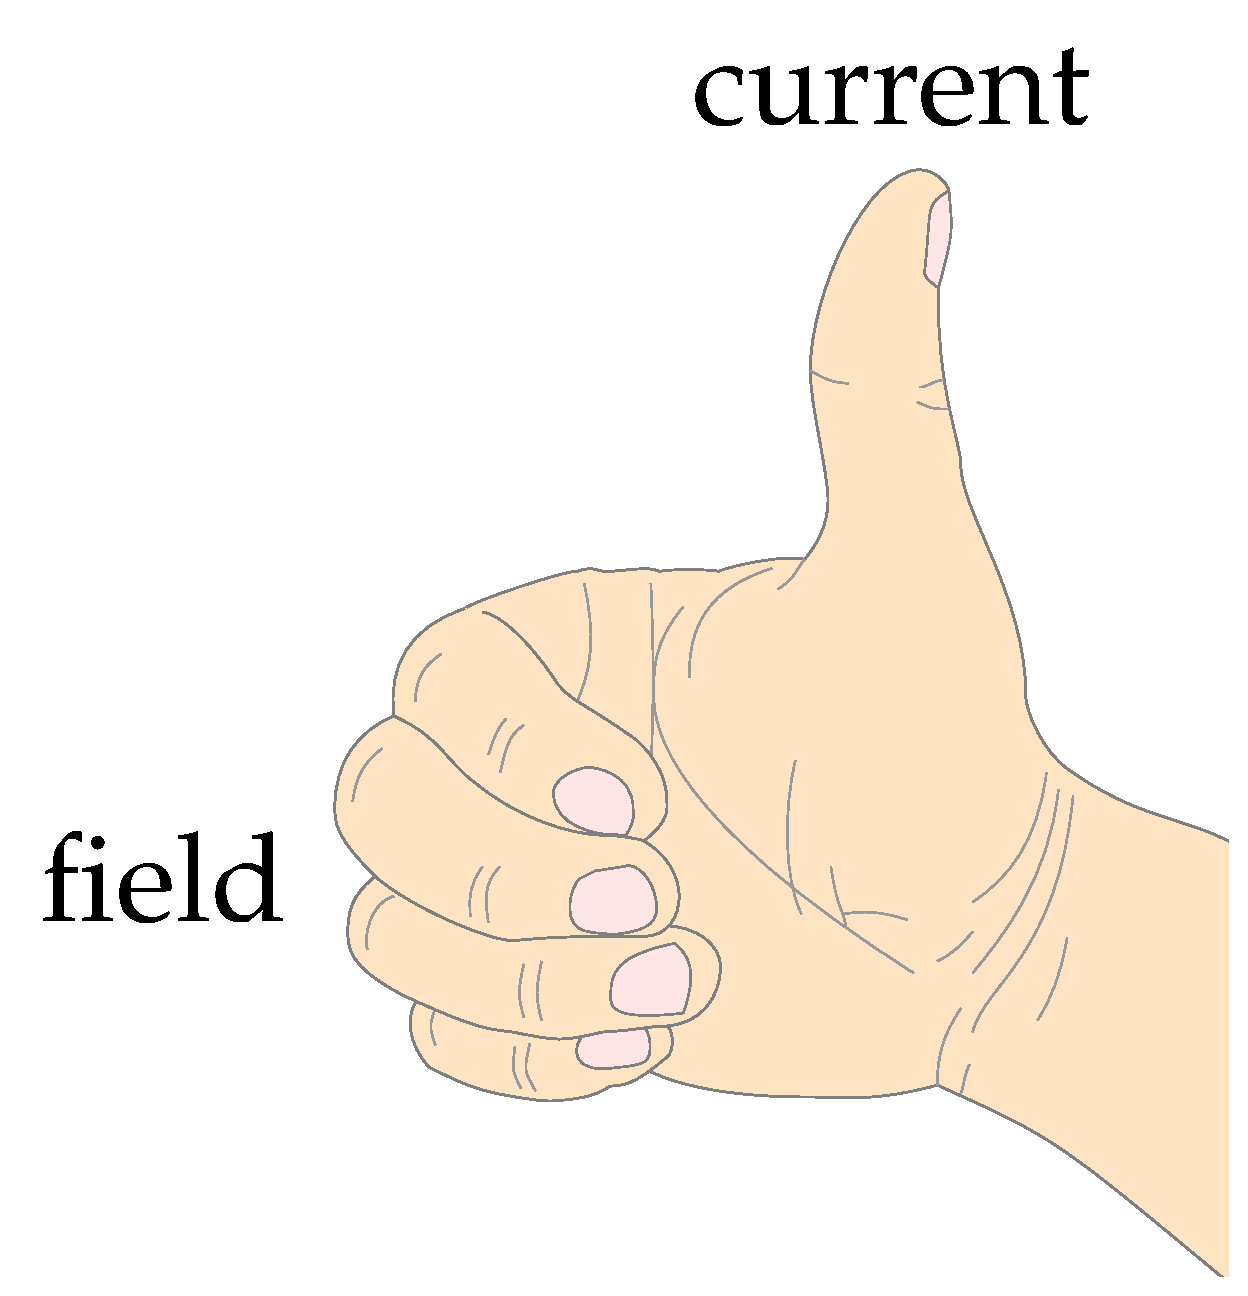
\includegraphics[height=108pt]{right-hand-straight.pdf}
\end{center}
\end{minipage}

\caption*{field due to a long straight current-carrying wire}
\end{figure}

\begin{figure}[ht]
\centering
\vspace*{-5pt}
\begin{minipage}{0.3\linewidth}
	\begin{center}
		\begin{tikzpicture}[scale=0.9,decoration={markings,mark=at position 0.75 with {\arrow{>}}}]
		\draw[very thick, postaction={decorate}] (0,0) ellipse (1.0 and 0.5);
		\draw (1.6,-0.5) node {current};
		\draw[white,fill] (-0.15,0.4) rectangle (0.15,0.6);
		\draw[white,fill] (-0.6,0.3) rectangle (-0.4,0.5);
		\draw[white,fill] (0.6,0.3) rectangle (0.4,0.5);
		\draw [very thick, blue, postaction={decorate}] (0,-2.4) -- (0,-0.7) (0,0) -- (0,2);
		\draw [very thick, blue, postaction={decorate}] (0.96,-2.4) [out=120,in=-84] to (0.54,-0.7) (0.5,0) [out=90,in=-110] to (0.9,2);
		\draw [very thick, blue, postaction={decorate}] (-0.96,-2.4) [out=60,in=-96] to (-0.54,-0.7) (-0.5,0) [out=90,in=-70] to (-0.9,2);
		\draw [very thick, blue, dashed] (0,-0.7) -- (0,-0.1);
		\draw [very thick, blue, dashed] (0.54,-0.7) [out=96,in=-90] to (0.5,0);
		\draw [very thick, blue, dashed] (-0.54,-0.7) [out=84,in=-90] to (-0.5,0);
		\draw (1.4,1.5) node {field};
		\end{tikzpicture}
	\end{center}
\end{minipage}
\begin{minipage}{0.4\linewidth}
	\begin{center}
		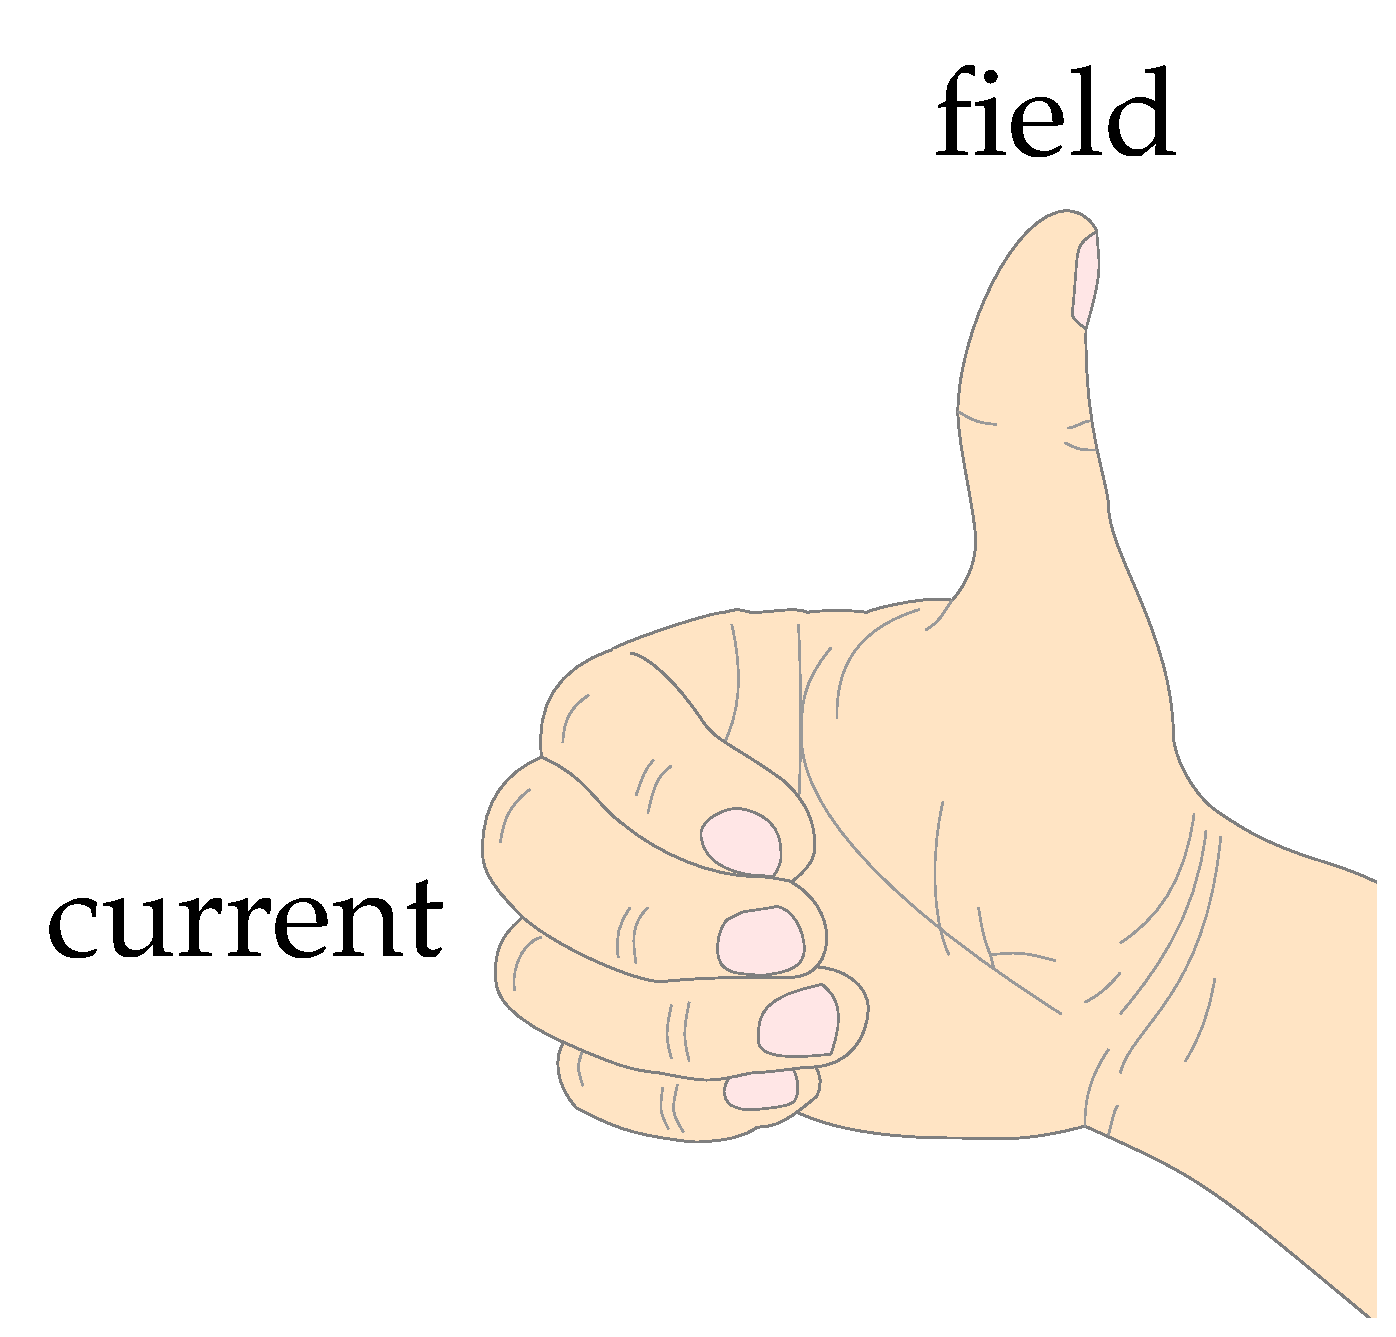
\includegraphics[height=120pt]{right-hand-circular.pdf}
	\end{center}
\end{minipage}
\vspace*{-10pt}
\caption*{field due to a circulating current}
\vspace*{-12pt}
\end{figure}

\cmt strength of the field is proportional to the current: $B \propto I$

for both straight wires
\footnote{The magnetic flux density generated by a current flowing in an infinitely long wire in free space is given by: $\boxed{B=\frac{\mu_0 I}{2\pi r}}$, $I$ is the electric current, $r$ is the perpendicular distance from the current, and $\mu_0 = 4\pi \times 10^{-7} \text{ T m A}^{-1}$ is a fundamental physical constant called the \emph{vacuum permeability}. ($\ast$)}
 and coils\footnote{The magnetic flux density at the centre of a current-carrying coil in free space is given by: $\boxed{B=\frac{\mu_0 NI}{L}}$, where $N$ is the number of turns, $I$ is the electric current flowing through the coil, $L$ is the length of coil, and $\mu_0$ is the vacuum permeability. ($\ast$)}
 , greater current means stronger field
 
\cmt strength of magnetic field can be increased with \emph{soft iron}

this is because \emph{ferromagnetic materials} (iron, cobalt, nickel) can attract magnetic field lines\footnote{If the straight wire is immersed in a material with \emph{relative permeability} $\mu_r$, then the field becomes: $B=\frac{\mu_0 \mu_r I}{2\pi r}$. Similarly, if a material with relative permeability $\mu_r$ is present, then the magnetic flux density inside a coil becomes: $B=\frac{\mu_0 \mu_r NI}{L}$. A good magnetic material (high permeability material), such as iron, has large $\mu_r$, and therefore can greatly intensify the magnetic field. ($\ast$)}

\subsubsection{solenoids \& electromagnets}

strength and polarity of the field due to a coil can be changed easily by tuning currents, so coils are widely used to create magnetic fields where needed

a current-carrying coil is also called a \keypoint{solenoid}

\begin{figure}[htp]
	\centering
	\vspace*{-3pt}
	\begin{minipage}{0.65\linewidth}
		\begin{center}
			\begin{tikzpicture}[yscale=0.5,xscale=0.6]
			\tikzstyle flines=[thick,blue,postaction={decorate},decoration={markings,mark=at position 0.56 with {\arrow{>}}}] % field line style
			\tikzstyle ct=[very thick,postaction={decorate},decoration={markings,mark=at position 0.54 with {\arrow{>}}}] % coil style
			
			\draw [flines] (3,0) -- (6.8,0);
			\draw [flines] (3,0.2) [out=10,in=210] to (6.5,1.35);
			\draw [flines] (3,-0.2) [out=-10,in=-210] to (6.5,-1.35);
			\draw [flines] (3,0.5) [out=20,in=240] to (6,3.5);
			\draw [flines] (3,-0.5) [out=-20,in=-240] to (6,-3.5);
			
			\draw [flines] (3,0.9) [out=60,in=0] to (0,3.6) [out=180,in=120] to (-3,0.9);
			\draw [flines] (3,-0.9) [out=-60,in=0] to (0,-3.6) [out=180,in=-120] to (-3,-0.9);
			\draw [flines] (2.5,1) [out=150,in=30] to (-2.5,1);
			\draw [flines] (2.5,-1) [out=-150,in=-30] to (-2.5,-1);
			\draw[ct] (-2.6,-3.5) --++ (0,3);
			
			\draw[thick,fill=white] (3,0) ellipse (0.35 and 1);
			\draw[thick,white,fill] (-3,-1) rectangle (3,1);
			\draw[thick,fill=white] (-3,0) ellipse (0.35 and 1);
			\draw[thick] (-3,-1) -- (3,-1);
			\draw[thick] (-3,1) -- (3,1);
			\foreach \k in {-2.5,-2.0,...,2.1} {\draw[ct] (\k,1) [out=60, in=-120] to (\k+0.4,-1);}
			\draw[very thick] (2.5,1) [out=60, in=-120] to (2.9,-1);
			\draw[white,fill] (2.6,-.978) rectangle (2.8,0);
			\draw[white,fill] (2.7,-1.1) rectangle (2.9,-1.022);
			\draw[very thick] (2.7,0.1) -- (2.7,-1);
			\draw[ct] (2.7,-1) --++ (0,-2.5);
			
			\draw [flines] (-6.8,0) -- (-3,0);
			\draw [flines] (-6.5,1.35) [out=-30,in=170] to (-3,0.2);
			\draw [flines] (-6.5,-1.35) [out=30,in=190] to (-3,-0.2);
			\draw [flines] (-6,3.5) [out=-60,in=160] to (-3,0.5);
			\draw [flines] (-6,-3.5) [out=60,in=200] to (-3,-0.5);
			
			\draw (2.8,-2.1) --++ (1.2,-0.8) node[below]{current};
			\node at (5.8,2) {field};
			\node at (3.6,1.4) {N};
			\node at (-3.6,1.4) {S};
			\end{tikzpicture}
		\end{center}
	\end{minipage}
	\begin{minipage}{0.3\linewidth}
		\begin{center}
		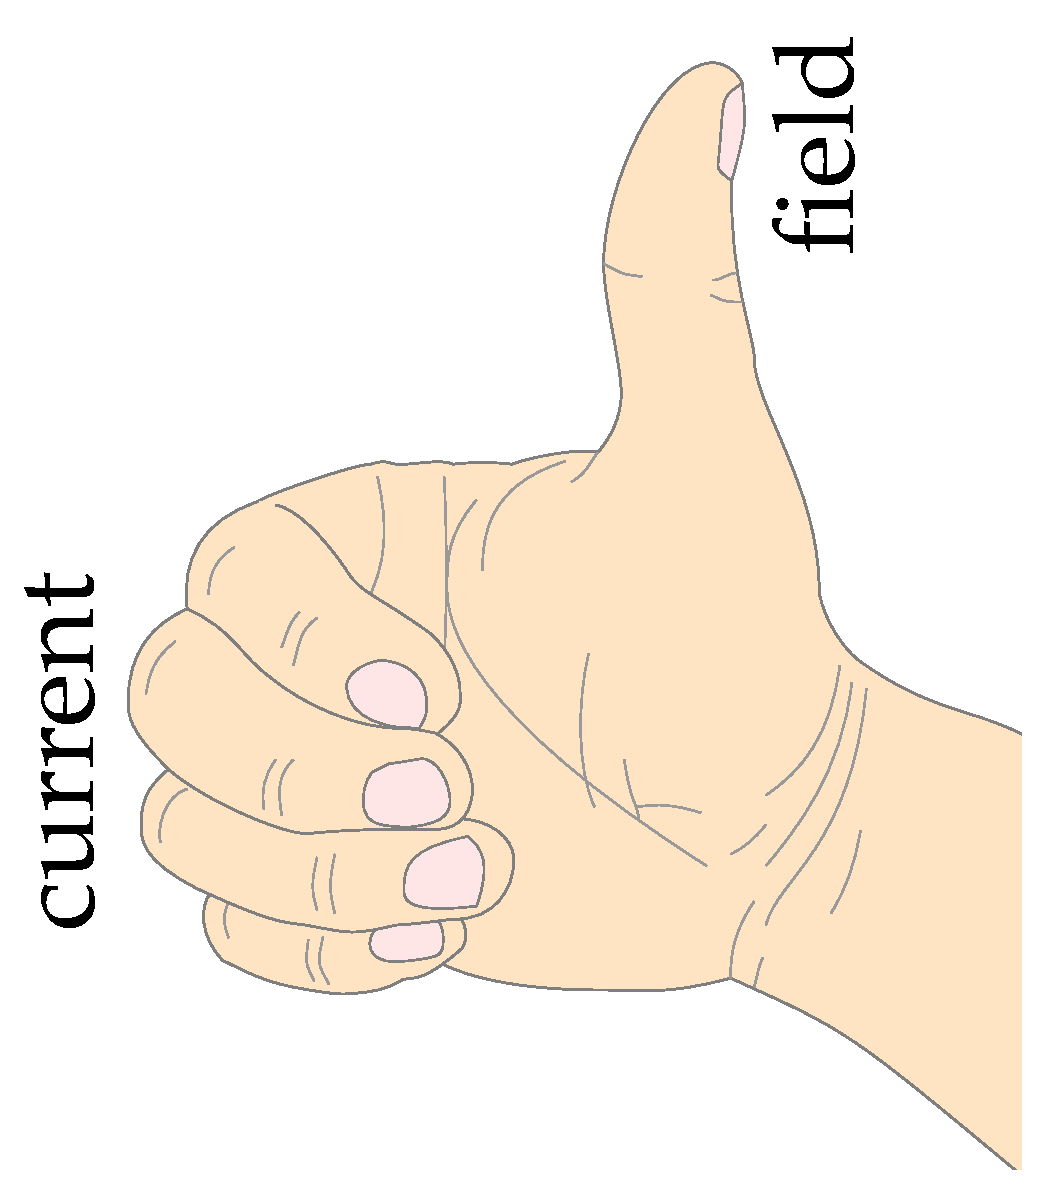
\includegraphics[height=108pt,angle=-90]{right-hand-coil.pdf}
		\end{center}
	\end{minipage}
	
	\caption*{magnetic field around a solenoid}
	\vspace*{-12pt}
\end{figure}

\cmt a solenoid generates a magnetic field similar to that of a bar magnet

useful to talk about the north and south poles of a solenoid

\cmt direction of magnetic field in a solenoid is given by the \keypoint{right-hand (grip) rule}\index{right-hand rule}

%\cmt a solenoid produces a \emph{uniform} magnetic field in its centre and near its poles

\cmt magnetic field produced by a solenoid can be controlled

current $I\up \ra $ stronger field, also number of turns $N\up\ra $ stronger field

\cmt inserting an \emph{iron core} inside greatly strengthens the field, this makes an \emph{electromagnet}

\question{Describe the magnetic field due to an alternating current through a solenoid.}


\subsection{magnetic force on current-carrying conductor}

\subsubsection{magnetic force on current-carrying conductor}

a current-carrying wire produces its own magnetic field, when it is surrounded by an external magnetic field, the two fields would interact $\ra$ a \keypoint{magnetic force}\index{magnetic field!magnetic force} on the conductor

\begin{wrapfigure}{r}{0.4\textwidth}
	\vspace*{-16pt}
	\centering
	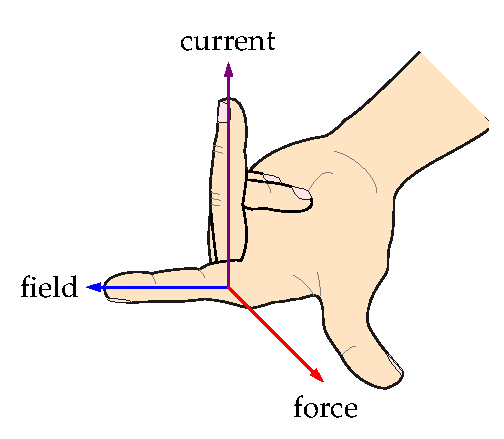
\includegraphics[height=135pt]{left-hand.pdf}
	
	Fleming's left-hand rule
	\vspace*{-16pt}
\end{wrapfigure}

\cmt direction of magnetic force on current can be worked out with \keypoint{Fleming's left-hand rule}\index{left-hand rule}\footnote{Figure credit again goes to \emph{Thomas S\"{o}ll} from the CTAN community.}

\cmt magnitude of magnetic force: $\boxed{F=BIL\sin\theta}$

$B$ is the magnetic flux density to be specified later

$I$ is the current, $\theta$ is the angle between $B$ and $I$

\cmt when $B \perp I$, magnetic force $F=BIL$

when $B \parallelslant I$, there is no magnetic force

when $B$ forms angle $\theta$ with $I$, only the \emph{perpendicular}

\noindent\emph{component} contributes to the force, giving rise to the $\sin\theta$ factor in the formula

\cmt magnetic force is perpendicular to both $B$ and $I$

\example{Determine the direction of the magnetic force acting. Check yourself.}
\begin{center}
	\begin{minipage}[b]{0.32\textwidth}
		\centering
		\begin{tikzpicture}[scale=0.45]
		\foreach \y in {-2,2} \foreach \x in {-2,2}
		\node at (\x,\y) {\large\textcolor{blue}{$\times$}};
		%magnetic fields
		\draw[ultra thick,->] (-3.5,0) -- (2,0) node[below]{\textcolor{black}{$I$}} ;
		\draw[ultra thick] (2,0) -- (3.5,0); %currents
		\draw[red,very thick,->] (0,0) -- (0,2.4) node[right]{$F$};
		\node[blue,above right] at (2,2) {$B$};
		\end{tikzpicture}
		
		(a)
	\end{minipage}
	\begin{minipage}[b]{0.32\textwidth}
		\centering
		\begin{tikzpicture}[scale=0.4]
		\foreach \y in {-2,2} \foreach \x in {-2,2}
		\draw[blue,fill] (\x,\y) circle(0.1);
		%magnetic fields
		\draw[ultra thick,->] (0,-3.5) -- (0,2) node[right]{\textcolor{black}{$I$}} ;
		\draw[ultra thick] (0,2) -- (0,3.5); %currents
		\draw[red,very thick,->] (0,0) -- (2.4,0) node[below]{$F$};
		\node[blue,above right] at (2,2) {$B$};
		\end{tikzpicture}
		
		(b)
	\end{minipage}
\begin{minipage}[b]{0.32\textwidth}
	\centering
	\begin{tikzpicture}[scale=0.64,decoration={markings,mark=at position 0.84 with {\arrow{>}}}]
	\foreach \y in {-2,2}
	{
		\draw[blue,thick,postaction={decorate}] (-3,\y) -- (3,\y);
	}
	%magnetic fields
	\node[blue] at (3.4,1) {$B$};
	\draw [very thick, postaction={decorate}] (-2,0) -- ++(0:4) node[right] {$I$};
	\node[red,below] at (0,-0.3) {$F=0$};
	\end{tikzpicture}
	
	(c)
\end{minipage}
\end{center}


\subsubsection{magnetic flux density} \label{sec:magnetic_flux_density}

rewrite $F=BIL\sin\theta$ as $B = \frac{F}{IL\sin\theta}$,we can now give a formal definition for flux density $B$:

\begin{ilight}
	\keypoint{magnetic flux density}\index{magnetic field!magnetic flux density} $B$ at a point is defined as the force acted per unit length on a conductor carrying a unit current at right angle to the magnetic field
\end{ilight}

\cmt flux density describes the strength of a magnetic field\footnote{Magnetic field strength is a different quantity, defined by $H=\frac{B}{\mu}$, with $\mu=\mu_0\mu_r$ being the \emph{magnetic permeability} of material. The naming of field strength $H$ and flux density $B$ are due to historical reasons.}

\cmt $B$ is measured in \keypoint{tesla}\index{tesla} (T)\footnote{Telsa is a very large unit. For example, the strength of a typical refrigerator magnet is of about $10^{-3} \text{ T}$, even the very strong superconducting coils used in MRI are of around $1\sim3 \text{ T}$.}: $[B]=\text{T}$, $1 \text{ T} = 1 \text{ N}\cdot\text{A}^{-1}\cdot\text{m}^{-1}$

\begin{ilight}
	if a wire of 1 m normal to the magnetic field that carries a current of $1\text{ A}$ experiences a force of $1\text{ N}$, then the magnetic flux density is $1\text{ T}$
\end{ilight}

\cmt $B$ is a \emph{vector} quantity, with both magnitude and direction


\example{A wire of 0.80 m carrying a current of 5.0 A is lying at right angles to a magnetic field, it experiences a force of 0.60 N, what is the flux density?}
	
\sol $B=\frac{F}{IL} = \frac{0.60}{5.0\times0.80} = 0.15 \text{ T} \quad $ (a field of over 0.1 T is actually quite strong!) \eoe


\newpage
\example{Torque on a rectangular metal frame in uniform magnetic field}

\begin{wrapfigure}{l}{0.36\textwidth}
	\vspace*{-12pt}
	\centering
	\begin{tikzpicture}[scale=0.96,decoration={markings,mark=at position 0.75 with {\arrow{>}}}]
	\draw[very thick, postaction={decorate}] (0,0) -- (0,3);
	\draw[very thick, postaction={decorate}] (0,3) -- (2,3);
	\draw[very thick, postaction={decorate}] (2,3) -- (2,0);
	\draw[very thick,postaction={decorate}] (0.8,-1.4) -- (0.8,0) -- (0,0);
	\draw[very thick,postaction={decorate}] (2,0) -- (1.2,0) --++ (0,-1.4);
	\foreach \y in {0.5,2.5} {
		\draw[blue,thick,->] (-1,\y) -- (3,\y);
	}
	\node[above,blue] at (3,2.5) {$B$};
	\node[below left] at (0,0) {$P$};
	\node[above left] at (0,3) {$Q$};
	\node[above right] at (2,3) {$R$};
	\node[below right] at (2,0) {$S$};
	\node[right] at (2,1) {$I$};
	\node[right,red] at (2.1,1.5) {$F$};
	\node[left,red] at (-0.1,1.5) {$F$};
	
	\draw[thick,<->] (-1.5,0) --++ (0,3) node[left, midway]{$L$};
	\draw[thick,<->] (0,3.6) --++ (2,0) node[midway,above]{$d$};
	
	\draw[white,fill] (2,1.5) circle (0.18);
	\draw[white,fill] (0,1.5) circle (0.18);
	\draw[red,thick] (2,1.5) circle (0.18);
	\draw[red,thick,fill] (2,1.5) circle (0.06) (0.6,1.3) node[above right]{$I$};
	\draw[red,thick] (0,1.5) circle (0.18);
	\draw[red,very thick] (-0.1,1.4) -- (0.1,1.6) (-0.1,1.6) -- (0.1,1.4);
	\end{tikzpicture}
	\vspace*{-8pt}
\end{wrapfigure}

a rectangular frame lies in parallel with the field

$QR, PS \parallelslant B$, so no force acting on these two sides

$PQ, RS \perp B$, so there is magnetic force $F=BIL$

using left-hand rule, we find $F_{PQ}$ acts into the paper, $F_{RS}$ acts out of the paper

this is a pair of equal but opposite forces

they produce a torque about central axis of frame: $\tau=Fd=BILd$, causing the frame to rotate\footnote{This effect allows engineers to build \emph{electric motors}, such as those in electric vehicles, washing machines, blenders, etc.}\eoe

\question{If the plane of the rectangular frame is at right angle to the magnetic field, describe the magnetic forces acting on each side and hence state what happens to the frame.}

\begin{wrapfigure}{r}{0.35\textwidth}
	\vspace*{-12pt}
	\centering
	\begin{tikzpicture}[scale=0.75]
	\draw[ultra thick] (-2.5,0) -- (-2.5,4) --++ (1,0) --++ (0,-3) --++ (3,0) --++ (0,3) -- (2.5,4) -- (2.5,0) -- cycle;
	\node at (0,4) {\large $\otimes$};
	\node[above] at (0,4.1) {$I$};
	\node at (2,3.6) {$N$};
	\node at (-2,3.6) {$S$};
	\draw[ultra thick] (-3,-2) rectangle (3,-0.1);
	\draw[thick] (-1.5,-1.6) rectangle (1.5,-0.5);
	\node at (0,-1.1) {\large 500.0 g};
	\end{tikzpicture}
	\vspace*{-12pt}
\end{wrapfigure}

\example{A U-shaped magnet is placed on a balance with a wire suspended above it as shown. Magnetic flux density between the poles is about 0.50 T. The part of the wire that is in the field is of length 8.0 cm. The balance initially shows a reading of 500.0 g. When a current of 10 A flowing into the paper is switched on, what is the new reading on the balance?}\label{ex-mag-balance}

\sol use left-hand rule, force on wire acts upwards

from \emph{Newton's third law}, reaction force on magnet acts downwards

so there will be an increase in the balance reading

magnitude of the force: $F=BIl = 0.50 \times 10 \times 8.0\times10^{-2} = 0.40 \text{ N}$

change in the mass reading: $\Delta m = \frac{F}{g} = \frac{0.40}{9.81} \approx 0.0407 \text{ kg} \approx 40.7 \text{ g}$

new reading on balance: $m_\text{new} = 500.0 + 40.7 = 540.7 \text{ g}$ \eoe

\question{If the current in Example \ref{ex-mag-balance} is replaced by a current of 6.0 A flowing out of the plane of the paper. What is the reading on the balance?}

\subsubsection*{force between long straight current-carrying wires}

\begin{center}
\begin{minipage}{0.3\linewidth}
\begin{center}
\begin{tikzpicture}[scale=0.84,decoration={markings,mark=at position 0.6 with {\arrow{>}}}]
\draw[ultra thick, postaction={decorate}] (-1.2,0) node[left]{$I_1$} (-1.2,-2) -- (-1.2,2);
\draw[ultra thick, postaction={decorate}] (1.2,0) node[right]{$I_2$} (1.2,-2) -- (1.2,2);
\end{tikzpicture}
\end{center}
\end{minipage}
\begin{minipage}{0.35\linewidth}
\begin{center}
\begin{tikzpicture}[scale=0.56,decoration={markings,mark=at position 0.4 with {\arrow{>}}}]
\draw[black,thick] (0,0) circle (0.25);
\draw[black,thick,fill] (0,0) circle (0.06) (0,0.2) node[above]{$I_1$};
\draw[black,thick] (3,0) circle (0.25);
\draw[black,thick,fill] (3,0) circle (0.06) (3,0.2) node[above left]{$I_2$};
\draw[thick, blue, postaction={decorate}] (4:3) arc [radius=3, start angle=5, end angle=356];
\draw[blue] (144:3.6) node{$B_1$};
\draw[red,thick,->] (3,0) -- (1.2,0) node[below]{$F_{21}$};
\end{tikzpicture}
\end{center}
\end{minipage}
\begin{minipage}{0.3\linewidth}
\begin{center}
\begin{tikzpicture}[scale=0.84,decoration={markings,mark=at position 0.6 with {\arrow{>}}}]
\draw[ultra thick, postaction={decorate}] (-1.2,0) node[left]{$I_1$} (-1.2,-2) -- (-1.2,2);
\draw[ultra thick, postaction={decorate}] (1.2,0) node[right]{$I_2$} (1.2,-2) -- (1.2,2);
\draw[red,thick,->] (1.2,0) -- (0.1,0) node[below right]{$F_{21}$};
\draw[red,thick,->] (-1.2,0) -- (-0.1,0) node[below left]{$F_{12}$};
\end{tikzpicture}
\end{center}
\end{minipage}
\end{center}

if we have two straight parallel wires carrying currents in the same direction

force acting on $I_2$ is due to magnetic field $B_1$ generated by $I_1$

from top view, $I_1$ creates a counter-clockwise $B_1$, so $I_2$ experiences an upward field

using left-hand rule, force acting on $I_2$ by $I_1$, denoted $F_{21}$\footnote{$F_{AB}$ denotes the force acted on object $A$ by object $B$.}, points to the left

since $F_{21}$ and $F_{12}$ are a pair of action-reaction, so $F_{12}$ points to the right


\begin{center}
\begin{minipage}{0.3\linewidth}
\begin{center}
\begin{tikzpicture}[scale=0.84,decoration={markings,mark=at position 0.6 with {\arrow{>}}}]
\draw[ultra thick, postaction={decorate}] (-1.2,0) node[left]{$I_1$} (-1.2,-2) -- (-1.2,2);
\draw[ultra thick, postaction={decorate}] (1.2,0) node[right]{$I_2$} (1.2,2) -- (1.2,-2);
\end{tikzpicture}
\end{center}
\end{minipage}
\begin{minipage}{0.35\linewidth}
\begin{center}
\begin{tikzpicture}[scale=0.56,decoration={markings,mark=at position 0.4 with {\arrow{>}}}]
\draw[black,thick] (0,0) circle (0.25);
\draw[black,thick,fill] (0,0) circle (0.05) (0,0.2) node[above]{$I_1$};
\draw[black,thick] (3,0) circle (0.25);
\draw[black,thick] (3,0.2) node[above left]{$I_2$};
\draw[black,thick] (3.13,0.13) -- (2.87,-0.13) (3.13,-0.13) -- (2.87,0.13);
\draw[thick, blue, postaction={decorate}] (4:3) arc [radius=3, start angle=5, end angle=356];
\draw[blue] (144:3.6) node{$B_1$};
\draw[red,thick,->] (3,0) -- (4.8,0) node[below]{$F_{21}$};
\end{tikzpicture}
\end{center}
\end{minipage}
\begin{minipage}{0.3\linewidth}
\begin{center}
\begin{tikzpicture}[scale=0.84,decoration={markings,mark=at position 0.6 with {\arrow{>}}}]
\draw[ultra thick, postaction={decorate}] (-1.2,0) node[right]{$I_1$} (-1.2,-2) -- (-1.2,2);
\draw[ultra thick, postaction={decorate}] (1.2,0) node[left]{$I_2$} (1.2,2) -- (1.2,-2);
\draw[red,thick,->] (1.2,0) -- (2.2,0) node[below left]{$F_{21}$};
\draw[red,thick,->] (-1.2,0) -- (-2.2,0) node[below right]{$F_{12}$};
\end{tikzpicture}
\end{center}
\end{minipage}
\end{center}

similar discussions apply for $I_1$ and $I_2$ flowing in opposite directions (left as exercise)

hence we come to an conclusion: \emph{parallel currents attract, and anti-parallel currents repel}\footnote{The S.I. unit for current, ampere, is defined using two long wires parallel to each other carrying the same current in the same direction. If the wires are separated by 1 m and the magnetic force experienced per metre is $2.0\times10^{-7}$ N, then the current is of 1 A.}

\question{A light coil of wire of several loops is suspended from a fixed point. When an electric current is switched on in the coil, state and explain the change in the separation between the loops.}

\question{Two long parallel wires carry currents of $I_1=$3.0 A and $I_2=$5.0 A in the same direction as shown. The flux density at a point at perpendicular distance $r$ from a straight long wire carrying current $I$ is given by $B=\frac{\mu_0 I}{2\pi r}$.}\label{q-pwires}



\begin{figure}[htp]
\centering
\begin{tikzpicture}[scale=1.2,decoration={markings,mark=at position 0.65 with {\arrow{>}}}]
\draw[very thick, postaction={decorate}] (0,0) --++ (0,4) node[pos=0.55, left]{$I_1$};
\draw[very thick, postaction={decorate}] (3,0) --++ (0,4) node[pos=0.55, left]{$I_2$};
\draw[gray,dashed,thick] (-2.5,1) --++ (1.5,2) --++ (6.5,0) --++ (-1.5,-2) --++ (-6.5,0); 
\end{tikzpicture}
\end{figure}

\begin{compactenum}
\item[(a)] Draw at least three lines to show the magnetic field due to $I_1$.

\item[(b)] State and explain the direction of force acting on $I_2$.

\item[(c)] Given that $I_1$ and $I_2$ are separated by 4.0 cm, what is flux density due to $I_1$ at $I_2$?

\item[(d)]  What is the magnetic force per unit length acting on $I_2$?

\item[(e)] What is the magnitude and the direction of the force per unit length acting on $I_1$?
	
\end{compactenum}

\question{If the current in one of the two wires in Question \ref{q-pwires} is replaced by an alternating current, then the two wires should begin to vibrate. However, the wires are not observed to move. Make some reasonable estimates and explain why the vibration is not observed.}







\subsection{magnetic force on charged particles}

electric currents are formed by moving charges, since current-carrying wires in a magnetic field experience force, charged particle moving in magnetic field should also experience force

\subsubsection{magnetic force on charged particles}

starting from $F=BIl\sin\theta$, let's substitute $I=nAqv \RA F=B(nAqv)l\sin\theta$

notice $n$ is the number density of charged particles, so $nAl$ together gives the total number

if we look at the force acting on \emph{one} charged particle, then $nAl=1$, so: $F=Bqv\sin\theta$\index{magnetic field!magnetic force}

\cmt magnitude of magnetic force on charged particle: $\boxed{F=Bqv\sin\theta}$ 

$B$ is magnetic flux density, $q$ is electric charge of the particle, $v$ is its velocity

$\theta$ refers to the angle between $B$ and $v$

\begin{wrapfigure}{r}{0.45\textwidth}
	\vspace*{-16pt}
	\centering
	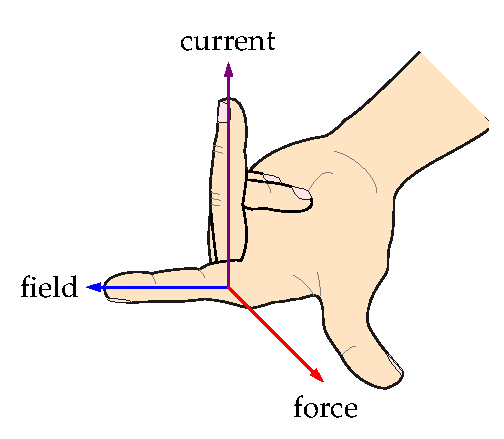
\includegraphics[height=135pt]{left-hand.pdf}
	
	Fleming's left-hand rule
	\vspace*{-16pt}
\end{wrapfigure}

\cmt direction of magnetic force can be determined using \emph{Fleming's left-hand rule}\index{left-hand rule}

for $+q$, current in same direction as $v$

for $-q$, current in opposite direction as $v$

\cmt force depends on \emph{perpendicular component} of $B$

if $v \perp B$, magnetic force $F=Bqv$

if $v \parallelslant B$, there is no magnetic force

when particle moves at angle $\theta$ to $B$, contribution to the force only comes from the \emph{perpendicular component}, giving rise to the $\sin\theta$ factor

\cmt magnetic force always perpendicular to both velocity $v$ and magnetic field $B$\footnote{Vector form of the formula: $\vec{F} = q\vec{v} \times \vec{B}$. ($\ast$)}

\example{Use the left-hand rule to find the direction of the magnetic forces acting on the following moving charges. Check yourself.}
\begin{center}
	\begin{minipage}[b]{0.45\textwidth}
		\centering
		\begin{tikzpicture}[scale=1]
		\draw[blue,dashed] (-2.7,-2.7) rectangle (2.7,2.7);
		\foreach \y in {-2,0,2} \foreach \x in {-2,0,2}
		\node at (\x,\y) {\large\textcolor{blue}{$\times$}};
		%magnetic fields
		\draw[purple,very thick,->] (-1.1,-1.2) --++ (1.5,0) node[midway,above]{$v$};
		\draw[red,very thick,->] (-1.1,-1.2) --++ (0,1.8) node[left]{$F$};
		\shade [ball color = orange] (-1.1,-1.2) circle (0.15);
		\node[below] at (-1.1,-1.4) {$+q$};
		\draw[purple,very thick,->] (1.2,1.2) --++ (0,-1.5) node[midway,right]{$v$};
		\draw[red,very thick,->] (1.2,1.2) --++ (-1.8,0) node[above]{$F$};
		\shade [ball color = green] (1.2,1.2) circle (0.15);
		\node[above] at (1.2,1.4) {$-q$};
		\node[blue,above right] at (2,2) {$B$};
		\end{tikzpicture}
		
		(a)
	\end{minipage}
	\begin{minipage}[b]{0.45\textwidth}
		\centering
		\begin{tikzpicture}[scale=1]
		\draw[blue,dashed] (-2.7,-2.7) rectangle (2.7,2.7);
		\foreach \y in {-2,0,2} \foreach \x in {-2,0,2}
		\draw[blue,fill] (\x,\y) circle(0.05);
		%magnetic fields
		\draw[purple,very thick,->] (-0.6,-1.2) --++ (110:1.4) node[midway,above right]{$v$};
		\draw[red,very thick,->] (-0.6,-1.2) --++ (20:1.8) node[below]{$F$};
		\shade [ball color = orange] (-0.6,-1.2) circle (0.15);
		\node[below] at (-0.6,-1.4) {proton};
		\draw[purple,very thick,->] (1,0.5) --++ (70:1.2) node[midway,right]{$v$};
		\draw[red,very thick,->] (1,0.5) --++ (160:1.8) node[above]{$F$};
		\shade [ball color = green] (1,0.5) circle (0.15);
		\node[below] at (1,0.3) {electron};
		\node[blue,above right] at (2,2) {$B$};
		\end{tikzpicture}
		
		(b)
	\end{minipage}
\end{center}

\subsubsection*{charged particles in electric \& magnetic fields}

in either electric field or magnetic field, charged particle may experience a force\footnote{The combination of electric and magnetic force on the charge due to electromagnetic fields is called the \emph{Lorentz force}\index{Lorentz force}: $\vec{F} = q(\vec{E} + \vec{v}\times \vec{B})$. If you have a good knowledge in maths, everything we cover in this section can be recovered from this vector equation. ($\ast$)}

in this section, we will compare the difference between electric field and magnetic field

\begin{center}
	{%\renewcommand{\arraystretch}{1.2}
		\begin{tabular}{|D{0.22\textwidth}|D{0.36\textwidth}|D{0.3\textwidth}|}
			
			\hline
			& electric field & magnetic field \\ \hline
			
			strength of the field & electric field strength $E$ & magnetic flux density $B$ \\ \hline
			
			magnitude of force & $F_E = Eq$ & $F_B=Bqv\sin\theta$ \\ \hline
			
			whether force depends on velocity & no dependence, acts equally on stationary or moving charges & depend on perpendicular component of velocity \\ \hline
			
			\multirow{2}{*}{direction of force} & $F_E \parallelslant E$ &  $F_B \perp B$ and $F_B \perp v$ \\
			
			& same as/opposite to $E$ for $+q$/$-q$ & use left-hand rule\\ \hline
			
			effect of force on motion of particle & can change both magnitude and direction of velocity & only changes direction of velocity, cannot change magnitude of velocity \\ \hline
			
			work done by force & work can be done, can define notions of potential and P.E. & magnetic force does no work for charged particles\\ \hline
			
	\end{tabular}}
\end{center}



\subsubsection{charged particle in uniform magnetic fields}

suppose a charged particle is moving at right angle to a uniform magnetic field

\begin{figure}[htp]
	\centering
	\begin{tikzpicture}[scale=0.65]
			\draw[blue, dashed] (-4,-4) rectangle (4,4);
			\foreach \x in {-3,0,3}{
				\foreach \y in {-3,0,3}{
					\node[draw,circle,blue,inner sep=0.8pt,fill] at (\x,\y) {};  }}
			\node[blue] at (-2.5,2.5) {$B$};
			\draw[thick,dotted] (0,0) circle [radius=2.5];
			\foreach \s in {80,200,310}
			{
				\draw [purple, thick, ->] (\s:2.5) -- ++(\s-90:2);
				\draw [purple] (\s-35:3.5) node{$v$};
				\draw [red, thick, ->] (\s:2.5) -- (\s:0.8);
				\draw [red] (\s+25:1) node{$F$};
				\shade [ball color = yellow] (\s:2.5) circle (0.25) node{\footnotesize$+$};
			}
	\end{tikzpicture}
	
	circular motion of a charged particle in uniform magnetic field
	
	\vspace*{-10pt}
\end{figure}

magnetic force $F_B$ always at right angle to motion, so $F_B$ keeps changing direction of velocity

uniform field means a constant force, so $F_B$ deflects the particle at the same rate

the particle should describe a \emph{circular} path!

\newpage

\vspace*{-\baselineskip}
\begin{ilight}
	for a charged particle moving in a uniform magnetic field, \emph{magnetic force provides centripetal force for circular motion}: $\boxed{Bqv = \frac{mv^2}{r}}$, or $\boxed{Bqv = m \omega^2 r}$
\end{ilight}

\cmt can solve for radius of the orbiting particles: $r=\frac{mv}{Bq}$

\begin{compactenum}

\item[-] $v\up \Rightarrow r\up$, faster particles take larger circles
	
\item[-] $B\up \Rightarrow r\down$, stronger magnetic field, larger centripetal force, smaller circles
	
\item[-] $m\up \Rightarrow r\up$, larger mass, larger inertia, so larger circles

\end{compactenum}
	
\cmt radius of curvature relates to charge-to-mass ratio (also called \emph{specific charge}\index{specific charge}) of the particle

rearrange the equation we have $\frac{q}{m}=\frac{v}{Br}$, which can be computed using experimental data

\example{An $\alpha$-particle travelling at $2.5\times10^4 \mps$ enters a region of uniform magnetic field. The field has flux density of 5.4 mT and is normal to direction of particle's velocity. What is the radius of $\alpha$-particle's path?}

\sol radius of circular arc: $r=\frac{mv}{Bq} = \frac{4\times 1.66\times10^{-27}\times2.5\times10^4}{5.4\times10^{-3}\times2\times1.60\times10^{-19}} \approx 0.096 \text{ m} \approx 9.6 \text{ cm}$ \eoe

\question{For an $\alpha$-particle and a $\beta$-particle entering the same uniform magnetic field at a same speed, compare the radius of their paths.}

\question{For a charged particle undergoing circular motion in a uniform magnetic field, show that its angular velocity is independent of the radius of its path.}

\question{If a charged particle enters a uniform magnetic field at an angle $\theta \neq 90^\circ$, state and explain the path of this particle. (Hint: think about components of its velocity.)}
	
\subsubsection{mass spectrometer}

a \keypoint{mass spectrometer}\index{mass spectrometer} is a device to measure the charge-to-mass ratio of charged particles

\begin{figure}[ht]
	\centering
	\begin{tikzpicture}[scale=0.72,decoration={markings,mark=at position 0.7 with {\arrow{>}}}]
	% electric fields
	\draw[orange,dashed,fill=orange!20] (-8,1.5) rectangle (-4,-1.5);
	\draw[ultra thick] (-8,-1.5) --++ (0,3);
	\draw[ultra thick] (-4,-1.5) --++ (0,1.3) (-4,1.5) --++ (0,-1.3);
	\draw (-6,-1) --++ (-1.2,-1.5) node[twoline,below]{accelerating voltage\\supply of p.d. $V$};
	% magnetic field
	\draw[dashed,blue,fill=blue!10] (0,1) rectangle (5,-9);
	\node[blue] at (3.6,-0.4){$B$};
%	\foreach \y in {0.167,-1.5,-3.167,-4.833,-6.5,-8.167} \foreach \x in {0.833,2.5,4.167}
%	\node[blue] at (\x,\y) {$\times$};
	\draw (4.5,-0.5) --++ (1.2,1.2) node[twoline,right]{uniform magnetic\\field region};
	% paths of particle beam
	\draw [thick,purple,postaction={decorate}] (0,0) arc(90:-90:4);
	\draw [thick,purple,postaction={decorate}] (0,0) arc(90:-90:3);
	\draw [thick,purple,postaction={decorate}] (-8,0) -- (-4,0);
	\draw [thick,purple,postaction={decorate}] (-4,0) -- (0,0);
	\node[purple,above] at (-2,0) {$v$};
	\shade [ball color = green] (-7,0) circle (0.2);
	\shade [ball color = green] (-3,0) circle (0.2);
	\draw[<->] (-0.3,0) --++ (0,-8) node[midway,left]{$d=2r$};
	% detectors
	\draw[gray!50,fill] (-1,-5) rectangle(-0.7,-9);
	\draw (-0.85,-6.5) --++ (-1,1) node[left,twoline]{particle\\detector};
	\end{tikzpicture}
	
	\caption*{deflection of two charged particles in a mass spectrometer}
	\vspace*{-12pt}
\end{figure}

charged particles accelerated through an electric field: $\frac{1}{2}mv^2 = qV$

they then enter a uniform magnetic field: $Bqv = \frac{mv^2}{r} \ra v=\frac{Bqr}{m}$ $\quad$

eliminating $v$: $v^2 = \frac{2qV}{m} = \frac{B^2 q^2 r^2}{m^2} \ra \frac{q}{m} = \frac{2V}{B^2 r^2}$

we can measure $V$, $B$, $r$ in practice, so the charge-to-mass ratio $\frac{q}{m}$ is worked out

different particles have different values of $\frac{q}{m}$, unknown particles can be identified

\question{In the figure above, two paths of deflected particles are shown. Give reasons why the radius of the circular path can be different.}

\question{If the particles sent into the mass spectrometer are positively-charged, in which direction should the magnetic field be applied?}

\question{A particle carrying a charge of $+e$ enters a uniform magnetic field of $8.8$ mT at right angles with an initial speed of $1.4\times10^5 \text{ m s}^{-1}$. It describes a semi-circle with diameter of 66 cm. (a) Find the mass of the particle. (b) Suggest possible composition of this particle.}

\subsubsection{cyclotron}\index{cyclotron}\label{ch-cyclotron}

a \keypoint{cyclotron} is a type of \emph{particle accelerator}

\begin{figure}[ht]
	\centering
	\begin{tikzpicture}[decoration={markings,mark=at position 0.6 with {\arrow{>}}}, scale=1.25]
	\def\gap{0.6}
	% magnetic fields
	\draw[thick, dashed, blue, fill=blue!10] (-2.6,0) arc(180:25:2.73) [out=-25, in = 100] to (10:3.2) arc(10:0:3.2) --cycle;
	\draw[thick, dashed, blue, fill=blue!10] (-2.6,-\gap) arc(180:360:2.9) -- cycle;
	% electric field
	\draw[thick, dashed, blue, fill=orange!20] (-2.6,0) rectangle (3.2,-\gap);
	% semi-circular paths
	\draw[thick, postaction={decorate}] (1,0) arc(0:180:1);
	\draw[thick, postaction={decorate}] (-1,-\gap) arc(180:360:1.414);
	\draw[thick, postaction={decorate}] (1.818,0) arc(0:180:1.732);
	\draw[thick, postaction={decorate}] (-1.636,-\gap) arc(180:360:2);
	\draw[thick, postaction={decorate}] (2.364,0) arc(0:180:2.236);
	\draw[thick, postaction={decorate}] (-2.108,-\gap) arc(180:360:2.449);
	% accelerating paths
	\foreach \x in {1.818,2.364,2.791} \draw[thick, postaction={decorate}] (\x,-\gap) --++ (0,\gap);
	\foreach \x in {-1, -1.636, -2.108} \draw[thick, postaction={decorate}] (\x, 0) --++ (0,-\gap);
	\draw[thick, postaction={decorate}] (2.791,0) --++(0,3);
	\draw[thick] (1,-\gap/2) --++(0,\gap/2);
	% proton source
	\draw[fill] (1,-\gap/2) circle(0.1);
	% nodes
	\draw (0.207, -\gap) ++ (200:2.6) -- (-4,0.8) (160:2.3) -- (-4,1) node[left,twoline]{magnetic field\\into the paper};
	\draw (-2.4,-\gap/2) -- (-3.6,-1) node[left,twoline]{high-frequency\\alternating\\electric field};
	\draw (1,-\gap/2) -- (3.2,-2.8) node[right,twoline]{proton\\source};
	\draw (2.791,2.2) -- (1,3.5) node[above, twoline]{outgoing beam of\\high-speed protons};
	\end{tikzpicture}
	
	\caption*{protons being accelerated in a cyclotron}
	
	\vspace*{-12pt}
\end{figure}

the idea is to make use of a magnetic field to guide moving charges into a spiral path between accelerations by an electric field

as the particle enters and leaves the region of electric field, it gains extra energy of $qV$

it then follows a semi-circular path under magnetic force and re-enters the electric field

polarity of the electric field is reversed so the particle continues to accelerate across the gap

energy of particle increases by $qV$, it then moves in a larger semi-circle in magnetic field

repeat this process, the particle leaves the exit port with very high speed



\cmt cyclotron frequency

for charged particles circulating in a uniform magnetic field: $Bqv=m\omega^2 r$

time to complete one full turn is: $T=\frac{2\pi r}{v} = \frac{2\pi}{v}\times\frac{mv}{Bq}\ra T=\frac{2\pi m}{Bq}$

this shows the period is independent of radius of the circular path!

if an alternating voltage is applied at frequency $f=\frac{Bq}{2\pi m}$, particles can be accelerated continuously at just the right time when they cross the gap

this frequency is known as the \emph{cyclotron frequency}

\question{Protons are accelerated in a cyclotron where the magnetic field region has a uniform flux density of 1.5 T and the voltage between the gap is 20 kV. (a) Find the frequency of the voltage supply needed. (b) Find the number of circles the protons must make in order to gain an energy of 10 MeV.}


\subsubsection{velocity selector}

\keypoint{velocity selector}\index{velocity selector} is a device to produce a beam of charged particles all with same speed $v$

\begin{figure}[ht]
	\centering
	\begin{tikzpicture}[xscale=0.9,yscale=0.8]
	\foreach \x in {-2,2}
	\foreach \y in {-1.5,1.5}
	\node[blue] at (\x,\y) {$\times$};
	\foreach \x in {-3,-1,...,3}
	\draw[orange,thick,->] (\x,3) -- (\x,-3);
	\node[blue] at (-2,2.1) {$B$};
	\node[orange] at (3.5,-2) {$E$};
	\draw[ultra thick] (-4,3) -- (4,3);
	\draw[ultra thick] (-4,-3) -- (4,-3);
	\draw[ultra thick] (0,-4.5) node[right]{$-$} -- (0,-3) (0,3) -- (0,4.5) node[right]{$+$};
	\draw [fill] (-4.2,0.2) rectangle (-4,3.6);
	\draw [fill] (-4.2,-0.2) rectangle (-4,-3.6);
	\draw [fill] (4.2,0.2) rectangle (4,3.6);
	\draw [fill] (4.2,-0.2) rectangle (4,-3.6);
	\shade [ball color = green] (-6.5,0) circle (0.1);
	\node[below,twoline] at (-6.5,-0.2) {electron\\beam};
	\draw[purple,thick,->] (-6.2,0) -- (-5,0) node[above,midway]{$v$};
	\draw[purple,thick,->] (-5,0) -- (6,0) node[above]{$v=\frac{E}{B}$};
	\draw[purple] (-4,0) [out=0,in=210] to (4,2);
	\node[purple,right] at (4.2,2) {$v<\frac{E}{B}$};
	\draw[purple] (-4,0) [out=0,in=160] to (4,-1.5);
	\node[purple,right] at (4.2,-1.5) {$v>\frac{E}{B}$};
	\shade [ball color = green] (0,0) circle (0.1);
	\draw[red,thick,->] (0,0.2) -- (0,2) node[above]{\textcolor{black}{$F_E=Eq$}};
	\draw[red,thick,->] (0,-0.2) -- (0,-2) node[below]{\textcolor{black}{$F_B=Bqv$}};
	
	\end{tikzpicture}
	
	\caption*{velocity selector}
	\vspace*{-12pt}
\end{figure}

let's consider a beam of electrons passing through a region where both uniform electric field and magnetic field are applied, electrons at desired speed $v$ are \emph{undeflected}

no net force acting on these electrons, so equilibrium between electric and magnetic force

{

\centering

$F_E = F_B \RA Eq = Bqv \RA \boxed{v=\frac{E}{B}}$

}

for particles entering the same region with higher speed, $F_B>F_E$, they deflect downwards

for particles entering the same region with lower speed, $F_B<F_E$, they deflect upwards

\question{If electrons at speed $v$ are undeflected when they pass through the velocity selector, what about a beam of $\alpha$-particles entering the same region at the same speed $v$?}

\question{A uniform magnetic field with flux density $6.0\times10^{-2} \text{ T}$ is applied out of the plane of the paper. A beam of protons are travelling into this region at a speed of $3.5\times10^4 \text{m s}^{-1}$. (a) In which direction do the protons deflect? (b) A uniform electric field is now applied in the same region so that the protons become undeviated. What is the strength and the direction of this electric field?}


\subsection{Hall effect}
when an electric current passes through a conductor surrounded by an external magnetic field perpendicular to the current, a transverse potential difference is produced

this phenomenon is known as the \keypoint{Hall effect}\index{Hall effect} (discovered by American physicist \emph{Edwin Hall} in 1879), the voltage difference is called the \keypoint{Hall voltage}

\vspace*{\baselineskip}

suppose magnetic field goes upward, current flows to the right (see figure), then charge carriers (assumed to be electrons for now) experience a magnetic force pointing out of paper

\begin{figure}[ht]
	\centering
	\begin{tikzpicture}[scale=1]
	\draw[thick] (-6,.5) -- ++(3,0); % current in
	\draw[thick,fill=gray!20] (-4,-1) -- ++(0,1) -- ++(3,2) -- ++(4,0) -- ++(0,-1)  -- ++(-3,-2) -- cycle;
	\draw[thick] (-4,0) -- (0,0) -- (3,2) (0,0) -- (0,-1); %conductor
	\draw[blue,thick,->] (-.5,-2.5) -- (-.5,-1) (-.5,1) -- ++(0,2) node[right]{$B$}; %magnetic fields
	\draw[thick,->] (1.5,.5) -- ++(3,0) node[above]{$I$}; % current out
	\shade [ball color = green] (-1.1,1) circle (0.12);
	\draw[thick,purple,->] (-1.1,1) -- ++(-1,0) node[above right]{$v$};
	\draw[thick,red,->] (-1.1,1) -- ++(-1,-.667) node[left]{$F_B$};
	\end{tikzpicture}
\end{figure}

this magnetic force causes a build-up of extra charge on front side of conductor, which produces an internal electric field $E$ inside conductor, i.e., a potential difference $V_H$ is formed

\begin{figure}[ht]
	\centering
	\begin{tikzpicture}[scale=1]
	\draw[thick] (-6,.5) -- ++(3,0); % current in
	\draw[thick,fill=gray!20] (-4,-1) -- ++(0,1) -- ++(3,2) -- ++(4,0) -- ++(0,-1)  -- ++(-3,-2) -- cycle;
	\draw[thick] (-4,0) -- (0,0) -- (3,2) (0,0) -- (0,-1); %conductor
	\draw[blue,thick,->] (-.5,-2.5) -- (-.5,-1) (-.5,1) -- ++(0,2) node[right]{$B$}; %magnetic fields
	\draw[thick,->] (1.5,.5) -- ++(3,0) node[above]{$I$}; % current out
	\shade [ball color = green] (-1.1,1) circle (0.12);
	\draw[thick,purple,->] (-1.1,1) -- ++(-1,0) node[above right]{$v$};
	\draw[thick,red,->] (-1.1,1) -- ++(-1,-.667) node[left]{$F_B$};
	\draw[thick,violet,->] (-1.1,1) -- ++(1,.667) node[right]{$F_E$};
	\foreach \ball in {-3.5,-2.5,-1.5,-0.5}{
		\shade [ball color = green] (\ball,-0.5) circle (0.12);
		\draw[thick] (\ball-0.05,-0.5) --++ (0.1,0);
	}
	\draw[thick,olive,<->] (-4.8,0) -- ++(3,2) node[midway,above left]{$V_H$};
	\draw[thick,olive,<-] (-0.8,.3) node[left]{$E$} -- ++(2.1,1.4);
	\draw[thick,<->] (.5,-1.35) -- ++(3,2) node[midway, below right]{$d$};
	\draw[thick,<->] (3.5,1) -- ++(0,1) node[midway, right]{$t$};
	\end{tikzpicture}
\end{figure}

as charge carriers accumulate on one side, Hall voltage opposes further migration of charges

steady $V_H$ is established when magnetic force and electric force are balanced: $Eq = Bqv$

\begin{compactenum}
	\item[-] strength of internal electric field is related to Hall voltage: $E=\frac{V_H}{d}$
	
	where $d$ is width of the conductor
	
	\item[-] drift velocity $v$ of particles is related to current $I$: $I=nAqv$
	
	where $A$ is cross section of conductor and $n$ is number density of charge carriers
\end{compactenum}


we now have: $\frac{V_H}{d}q = Bq \frac{I}{nAq} \ra V_H = \frac{BId}{nAq}$

note that cross section $A=dt$, where $t$ is thickness of conductor as shown

we therefore obtain an useful expression for Hall voltage: $ V_H = \frac{BId}{n(td)q} \ra \boxed{V_H = \frac{BI}{ntq}}$ 

\cmt to produce noticeable $V_H$, we want smaller $n$ and smaller $t$

\begin{compactenum}
	\item[-] $n\downarrow \ra$ few free charge carriers $\ra$ \emph{semi-conductors} are preferable

	\item[-] $t\downarrow \ra$ small thickness $\ra$ \emph{thin slice} of component is preferable

\end{compactenum}

\cmt polarity of $V_H$ is determined by nature of charge carries
	
charge carriers can be \emph{free electrons} (negatively charged) or \emph{holes} (positively charged)
	
then Hall voltage induced would have opposite polarity

\cmt if current $I$ forms angle $\theta$ with flux density $B$, again only perpendicular component matters

expression for Hall voltage becomes: $V_H = \frac{BI}{ntq}\sin\theta$
	
\cmt apply a fixed current in a conductor, $V_H$ is proportional to $B$
	
so magnetic flux density can be calculated once we find $V_H$
	
one can make use of Hall effect to build a \emph{Hall probe}, a device used to measure flux density $B$

when using a Hall probe, one should rotate and record the greatest voltage reading to ensure the current applied is at right angle to the external magnetic field

\question{Why is it difficult to detect Hall voltage in a thin slice of copper?}

\question{A Hall probe is placed near to one end of a strong magnet. State and explain the variation in the Hall voltage as the probe is rotated for one complete revolution.}
	

\section{Electromagnetic Induction}

\subsection{magnetic flux}

\rcyskip

\begin{ilight}
	\keypoint{magnetic flux} is defined as the product of a closed area and the magnetic flux density going through it at right angles: $\boxed{\phi=BA\cos\theta}$\index{magnetic field!magnetic flux}
\end{ilight}

\begin{wrapfigure}{r}{0.33\linewidth}
	\centering
	\begin{tikzpicture}[scale=1.25]
	
	\foreach \y in {-1.5,-0.75,0,0.75,1.5} \draw[blue,thick] (-1.5,\y-.6) -- (0,\y);
	\draw[very thick, fill=gray!25] (0,0) ellipse (0.6 and 1.2);
	\node at (-0.2,0.3) {$A$};
	\foreach \y in {-1.5,-0.75,0,0.75,1.5} \draw[blue,thick,->] (0,\y) -- (1.5,\y+0.6);
	\draw[thick,dashed] (0,0) -- ++(1.5,0);
	\draw[thick] (.8,0) arc(0:21.8:0.8);
	\draw (0,0) ++ (10.5:1) node {$\theta$};
	\node[blue] at (1.7,1) {$B$};
	\end{tikzpicture}
\end{wrapfigure}

\cmt unit for magnetic flux: $[\phi] = \text{Wb}$, $1\text{ WB} = 1 \text{ T}\cdot\text{m}^2$

\cmt if magnetic field is perpendicular to the area

magnetic flux simply becomes: $\boxed{\phi=BA}$

\cmt for a coil with $N$ turns, total magnetic flux is

{

\centering

$\boxed{\Phi = N\phi = NBA}$

}

this is called \keypoint{magnetic flux linkage}

\cmt magnetic flux $\phi$ can be graphically thought as the number of field lines through area $A$

cutting of field lines means a change in flux

\cmt change in flux can be caused by many processes, for example

\begin{compactenum}
	\item[-] moving a magnet towards/away from a coil
	
	\item[-] varying current in a solenoid/electromagnet
	
	\item[-] inserting an iron core into a solenoid/electromagnet
	
	\item[-] pushing a straight conductor through a magnetic field
	
	\item[-] rotating a coil in a magnetic field
	
	\item[-] $\cdots$
\end{compactenum}

\question{Explain why the processes mentioned above would give rise to a change in magnetic flux.}


\subsection{laws of electromagnetic induction}

electromagnetic induction is the phenomena that magnetism produces electricity\index{electromagnetic induction}

the laws of electromagnetic induction were discovered by \emph{Michael Faraday} and \emph{Heinrich Lenz} in the 1830s, and later described mathematically by \emph{James Clerk Maxwell}

we will study in what conditions voltages and currents could be induced, and how to find their magnitudes and polarities

\subsubsection{Faraday's law}

\rcyskip

\begin{ilight}
	\keypoint{Faraday's law}\index{Faraday's law} states that induced e.m.f./voltage is proportional to rate of change in magnetic flux (linkage): $\boxed{\mathcal{E} \propto \frac{\Delta \Phi}{\Delta t}}$
\end{ilight}

\cmt Faraday's law gives the \emph{magnitude} of the induced e.m.f.

the key here is the \emph{change} in flux: as long as flux changes, e.m.f. will be induced

\cmt if $\mathcal{E}$, $\Phi$, $t$ are all given in SI units, this proportional relation becomes an identity: $\boxed{\mathcal{E} = \frac{\Delta \Phi}{\Delta t}}$

\example{A coil of 80 turns is wound tightly around a solenoid with a cross-sectional area of 35 cm$^2$. The flux density at the centre of the solenoid is 75 mT. (a) What is the flux linkage in the coil? (b) The current in the solenoid is \emph{reversed} in direction in a time of 0.40 s, what is the average e.m.f. induced?}

\sol flux linkage: $\Phi = NBA = 80 \times 75\times10^{-2} \times 35 \times 10^{-4} = 0.21 \text{ Wb}$

average e.m.f. induced: $\mathcal{E} = \frac{\Delta \Phi}{\Delta t} = \frac{(+\Phi)-(-\Phi)}{\Delta t} = \frac{2\times 0.21}{0.40} = 1.05 \text{ V}$ \eoe

\subsubsection{Lenz's law}

\rcyskip

\begin{ilight}
	\keypoint{Lenz's law}\index{Lenz's law} states that induced e.m.f. or current is always in the direction to produced effects that \emph{oppose} the change in flux that produced it 
\end{ilight}

\cmt Lenz's law gives the \emph{polarity} of the induced current

the key here is the nature dislikes any change in flux: effects of induced current always \emph{oppose} the cause of its production

\cmt Lenz's law is a consequence of the conservation of energy

since induced current dissipates electrical energy as heat, it must cause loss of original forms of energy possessed by the system

if the change in flux is caused by motion, then magnetic force on/by the induced current must \emph{resist} this motion


\example{A coil of 200 turns is connected to a resistor $R=4.0$ $\Omega$. The coil has a diameter 10 cm. Initially a bar magnet is at great distance from the coil. The magnet is then inserted into the coil and field inside coil becomes 0.40 T. The process occurs within a duration of 2.0 s. }

\begin{figure}[ht]
	\centering
		\begin{circuitikz}[european resistors, scale=0.72]
		\tikzstyle ct=[thick] % coil style
		\draw[thick,fill=white] (3,0) ellipse (0.35 and 1);
		\draw[thick,white,fill] (-3,-1) rectangle (3,1);
		\draw[thick,fill=white] (-3,0) ellipse (0.35 and 1);
		\draw[thick] (-3,-1) -- (3,-1);
		\draw[thick] (-3,1) -- (3,1);
		\foreach \k in {-2.5,-2.0,...,2.1} {\draw[ct] (\k,1) [out=60, in=-120] to (\k+0.4,-1);}
		\draw[ct] (2.5,1) [out=60, in=-120] to (2.9,-1);
		\draw[white,fill] (2.6,-.978) rectangle (2.8,0);
		\draw[white,fill] (2.7,-1.1) rectangle (2.9,-1.022);
		\draw[ct] (-2.6,-1) -- (-2.6,-3.5) to[R=$R$] (2.7,-3.5) -- (2.7,0);
		
		\draw [fill=blue!70] (-9,-0.5) rectangle (-7.5,0.5);
		\draw [fill=red] (-7.5,-0.5) rectangle (-6,0.5);
		\node at (-8.25,0) {\large \textcolor{white}{S}};
		\node at (-6.75,0) {\large \textcolor{white}{N}};
		\draw[ultra thick, blue,->,dashed] (-5.5,0) -- (-3.5,0);
	\end{circuitikz}
\end{figure}

\noindent (a) What is average induced e.m.f. in the coil? (b) What is average induced current through resistor $R$? (c) In which direction does this current flow?


\sol change in flux linkage: $\Delta \Phi = NBA - 0 = 200\times0.40\times\pi \times 0.050^2 \approx 0.628 \text{ Wb}$

average e.m.f. induced: $\mathcal{E} = \frac{\Delta \Phi}{\Delta t} = \frac{0.628}{2.0} \approx 0.314 \text{ V}$

\eqyskip average current induced: $I = \frac{\mathcal{E}}{R} = \frac{0.314}{4.0} \approx 0.0785 \text{ A}$

as magnet approaches, coil experiences an increasing flux to the right

according to Lenz's law, field due to induced current acts to the left to oppose the change

alternatively, left side of the coil should behave as a north pole to oppose motion of magnet

use right-hand rule, we find induced current flows through $R$ to the right

\question{If the magnet is now pulled away from the coil, state ad explain the direction of the induced current.}

\newpage

\example{Two parallel metal tracks are separated by a distance of $L=45$ cm and placed in a uniform magnetic field of 0.80 T. The tracks are connected to a resistor $R=6.0$ $\Omega$. A long metal rod is being pushed under an external force at $v=3.0 \mps$ along the tracks as shown.}\label{ex-cuttingFL}

\begin{figure}[ht]
	\centering
	\begin{circuitikz}[european resistors, scale=0.9]
		\draw[thick] (0,1) --++ (10,0);
		\draw[thick] (-1,-1) --++ (10,0);
		\draw[ultra thick, gray] (-1,-1.5) -- (0.5,1.5);
		\draw[ultra thick,->,red] (-0.25,0) --++ (1.5,0) node[midway,above]{$v$};
		\draw[<->] (-1.5,-1) -- (-0.5,1) node[midway,above,rotate=63.43]{$L$};
		\foreach \x in {2,4,6,8} \draw[->,thick, blue] (\x,-2.4) -- (\x,-1.2) (\x,0) --++(0,2);
		\node[blue] at (6.5, 2) {$B$};
		\draw (10,1) [out=0,in=75] to (12,1) to[R=$R$] (11,-1) [out=255,in=0] to(9,-1);  
	\end{circuitikz}
\end{figure}

\noindent (a) What is the induced current through resistor? (b) In which direction does this current flow? (c) For the rod to travel at constant speed, what is magnitude of external force required?


\sol change of flux in time interval $\Delta t$ is: $\Delta \phi = \Delta (BA) = B \Delta A = BL v\Delta t$

e.m.f. induced: $\mathcal{E} = \frac{\Delta \phi}{\Delta t} \ra \boxed{\mathcal{E} = BLv}$

\eqyskip induced current: $I = \frac{\mathcal{E}}{R} = \frac{BLv}{R} = \frac{0.80\times0.45\times3.0}{6.0} = 0.18A$

according to Lenz's law, magnetic force on induced current opposes the rod's motion of cutting field lines, so magnetic force acts to the left

using Fleming's left-hand rule, we find induce current flows in anti-clockwise direction

if rod travels at constant speed, then equilibrium between external push and magnetic force

external force required: $F_\text{ext} = F_B = BIL = 0.80 \times 0.18 \times 0.45 \approx  0.065 \text{ N}$ \eoe

\question{In Example \ref{ex-cuttingFL}, can you find alternative arguments to determine the direction of the current induced as the rod cuts through the magnetic field?}

\subsubsection*{Hall voltage \& induced voltage in a coil}
	
in this section, we compare readings on voltmeter connected to a Hall probe and a coil
		
Hall probe picks up voltage proportional to flux density: $V_H \propto B$
		
coil picks up induced e.m.f. proportional to \emph{rate of change} in flux: $\mathcal{E} \propto \frac{\dd \Phi}{\dd t}$
		
\question{If a Hall probe is placed near a permanent magnet, what voltage do you measure? If a small coil is placed in the same field, state and explain whether you can measure a non-zero voltage in the coil. If not, state three different ways in which you can produce a voltage.}

\begin{wrapfigure}{r}{0.42\textwidth}
	\centering
	\vspace*{-8pt}
	\begin{tikzpicture}[xscale=0.8,yscale=0.7]
		\draw[<->] (0,3) node[left]{$I$} -- (0,0) -- (6,0) node[below]{$t$};
		\draw (0,-2) -- (0,0);
		\draw[thick,blue] (0,0) [out=70, in=180] to (2,2) -- (3.5,2) -- (3.8,-1.6) -- (6,-1.6);
	\end{tikzpicture}
	\vspace*{-20pt}
\end{wrapfigure}

\question{A Hall probe is placed near one end of a solenoid that carries a varying current as shown in the graph. (a) Sketch the variation of Hall voltage with time. (b) If Hall probe is replaced by a small coil parallel to the solenoid's end, sketch the variation of the voltage induced in the coil.}


\subsection{applications of electromagnetic induction}

\subsubsection{magnetic braking}

induction brakes make use of induced current to dissipate kinetic energy of a moving object

in this section, we will look at two simple demonstrations, but the principle can be used in braking system of high-speed trains, roller-coasters, etc.

\subsubsection*{the damped pendulum}

a metal disc can swings freely between the poles of an electromagnet

when the electromagnet is switched on, the disc comes to rest very quickly

\begin{figure}[ht]
\centering
\begin{tikzpicture}[scale=0.6]
% disc
\draw [thick] (0,6) ++ (-120:6) ++ (0,0.1) --++ (60:6) arc(150:-30:0.1) --++ (240:6);
\draw [thick,fill=gray!50] (0,6) ++ (-120:6) circle (1.2);
\draw [very thick, gray,dashed] (0,6) ++ (-60:6) circle (1.2);
\draw [purple,very thick,dashed,<->] (0,6) ++ (-75:6) arc(-75:-105:6);
% poles of EM magnet
\draw[thick] (0,1) rectangle (3,2.5);
\draw[thick] (-3,-1) -- (0,-1) -- (0,-2.5);
\draw[thick] (0,2.5) --++ (30:3);
\draw[thick] (3,2.5) --++ (30:2.7);
\draw[thick] (3,1) --++ (30:3);
\draw[thick] (-3,-1) --++ (210:3);
\draw[thick] (0,-1) --++ (210:4);
\draw[thick] (0,-2.5) --++ (210:3);
% nodes
\draw (3,1.75) ++(30:0.8) --++ (-30:2.5) node[twoline,below right]{poles of an\\electromagnet};
\draw (0,-1.75) ++(210:0.8) --++ (16:6.2);
\draw (0,6) ++ (-120:6) ++ (-0.5,0) --++ (150:3) node[left]{metal disc};
\end{tikzpicture}

%oscillation of pendulum dies away quickly due to drag force on eddy currents
\end{figure}


as disc moves in and out of field, change in flux gives rise to e.m.f induced

note that different parts of the disc experience different rates of change in flux, different e.m.f. is induced in different parts for the disc


this causes circulating currents flowing in the disc, called \keypoint{eddy currents}

\begin{compactenum}
	\item[-] vibrational energy is lost as heat due to the eddy currents induced
	
	\item[-] magnetic force on induced current causes damping
\end{compactenum}

so amplitude of oscillation decreases quickly

\subsubsection*{falling magnet}

suppose we drop two strong magnets down a plastic tube and a copper tube

\begin{figure}[ht]
	\centering
	\begin{tikzpicture}[scale=0.7]
	\draw[thick] (-2,0) ellipse (1 and 0.4) ellipse (0.9 and 0.36);
	\draw[thick] (-2,-5) ellipse (1 and 0.4);
	\draw[white,fill] (-3,-5) rectangle (-1,-4.5);
	\draw[thick] (-3,0) -- (-3,-5) (-1,0) -- (-1,-5);
	\draw[thick] (2,0) ellipse (1 and 0.4) ellipse (0.9 and 0.36);
	\draw[thick] (2,-5) ellipse (1 and 0.4);
	\draw[white,fill] (3,-5) rectangle (1,-4.5);
	\draw[thick] (3,0) -- (3,-5) (1,0) -- (1,-5);
	\draw[thick,fill=gray!30] (-2.4,1) rectangle (-1.6,3);
	\draw[thick,fill=gray!30] (2.4,1) rectangle (1.6,3);
	\draw (-2,2.4) -- (-0.5,4) (2,2.4) -- (0.5,4) (0,4) node[twoline, above]{strong\\magnets};
	\draw (-2,-3) --++ (-2.5,1) node[left,twoline]{plastic\\tube};
	\draw (2,-3) --++ (2.5,1) node[right,twoline]{copper\\tube};
	\end{tikzpicture}
	
	%it takes much longer for magnet to fall through copper tube
\end{figure}

as magnet falls, tube experiences change in flux, so e.m.f is induced

since plastic is an insulator, so no current flows in plastic tube, magnet undergoes free fall

but in the conducting copper tube, eddy current is induced in the tube

\begin{compactenum}
	\item[-] energy is lost as heat due to induced current, not all G.P.E. converted into K.E.
	
	\item[-] induced current exerts magnetic force on magnet to oppose its motion, acceleration $a<g$
\end{compactenum}

so magnet falls more slowly through the copper tube

\begin{wrapfigure}{r}{0.42\textwidth}
\centering
\begin{circuitikz}[european resistors,scale=0.75]
	% spring and magnet
	\draw[ultra thick] (-1,3.5) -- (1,3.5);
	\draw[thick, decorate, decoration={coil,amplitude=4pt, segment length=5pt}] (0,3.5) -- (0,1.5);
	\draw[thick, fill=gray!30] (-0.3,-0.5) rectangle (0.3,1.5);
	\draw[thick, fill=white] (-1,0) rectangle (1,-3.1);
	% coil
	\foreach \y in {-0.4,-0.7,...,-2.6} {
		\draw[thick] (-1,\y+0.1) [out=200, in=20] to (1,\y-0.1);
	}
	% circuit
	\draw[thick] (-1,-2.7) [out=200, in=180] to (0,-2.8) -- (1,-2.8) to[R=$R$] (3.6,-2.8);
	\draw[thick] (1,-0.2) -- (2,-0.2) --++ (30:0.7) (2.7,-0.2) -- (3.6,-0.2) -- (3.6,-2.8);
	% labels
	\draw (0,2.5) --++ (1.5,0.8) node[right]{spring};
	\draw (0,1) --++ (1.5,0.8) node[right]{magnet};
	\draw (-0.4,-0.7) --++ (-1.5,0.8) node[left]{coil};
	\node[above] at (2.1,0) {$S$};
\end{circuitikz}

\end{wrapfigure}

\question{A magnet is suspended from the free end of a spring. When displaced vertically and released, the magnet can oscillate in and out of a coil (see diagram). The switch $S$ is initially open, there is negligible change in the amplitude. However, when the switch is closed, the amplitude is seen to decrease quickly. Explain the reasons.}

\subsubsection{the generator} \label{subsection:generators}

imagine a coil rotates with constant angular speed $\omega$ in a uniform magnetic field $B$

\begin{wrapfigure}{r}{0.45\textwidth}
	\vspace*{-8pt}
	\centering
	\begin{tikzpicture}[scale=1,decoration={markings,mark=at position 0.75 with {\arrow{>}}}]
	\draw[very thick,postaction={decorate}] (0,2.1) ellipse (0.5 and 0.2);
	\draw[white,fill] (-0.15,2.1) rectangle (0.15,2.5) node[right]{\textcolor{black}{$\omega$}}; 
	\foreach \y in {-1.2,0,1.2}
	{
		\draw[blue,thick] (-2,\y) -- (-0.8,\y);
		\draw[blue,thick,->] (0,\y) -- (2,\y);
	}
	
	\draw[blue] (1.8,0.6) node{$B$};
	\draw[very thick] (-0.6,-1.8) -- (0.6,-1.2) -- (0.6,1.8) -- (-0.6,1.2) -- cycle;
	\draw[thick,dashed] (0,-2.1) -- (0,2.5);
	\draw[thick,dashed] (0,0) -- (1.2,0.6);
	\draw (0.8,0) arc(0:26.565:0.8);
	\node at (13:1) {$\theta$};
	
	\end{tikzpicture}
\end{wrapfigure}

let's assume that the coil initially lies in parallel to the field, i.e., $\theta=0$ at $t=0$

at time $t$, coil forms an angle $\theta=\omega t$ with the magnetic field (see diagram)

magnetic flux linkage through coil is:

{

\centering

$\Phi = NBA \sin\theta = NBA \sin \omega t$

}

magnitude of induced e.m.f. is: 

{
	
\centering

$\mathcal{E} = \frac{\dd \Phi}{\dd t} = \omega NBA \cos \omega t$

}

this is a sinusoidal voltage with maximum value: $\mathcal{E}_\tmax = \omega NBA$

for a coil rotating in a magnetic field like this, an \emph{alternating current} is generated

this is basically how a \emph{generator}\index{generator} works

in practice, it is a strong electromagnet rotating inside a large coil to generate electricity

\question{State and explain the effect on the voltage generated if the coil rotates faster.}

\question{For the coil rotating at a uniform angular speed in a uniform magnetic field, is the magnetic flux in phase with the e.m.f. generated? If not, what is the phase difference?}

\question{Does the generator output the maximum voltage when the rotating coil is in parallel to the magnetic field or when the coil is at right angle to the field?}

\subsubsection{electromagnetic gun}

a coil of wire of many turns is wound on a hollow tube

a light copper ring that can move freely along the tube is placed on the coil

let's find out what happens to the ring when a high-voltage supply is switched on

\begin{figure}[htp]
\centering
\begin{tikzpicture}[scale=0.75]
% tube base
\draw[fill=white] (0,0) ellipse (2 and 1);
% solenoid
\foreach \idx in {0.8,0.9,...,2} \draw[fill=gray!25] (0,\idx) ellipse (2.4 and 1.2); 
\draw[fill=white] (0,2) ellipse (2 and 1);
\draw[white,fill] (-2,2) rectangle (2,4);
\draw (-2,1.95) --(-2,3.5) (2,1.95) -- (2,3.5); 
% ring
\draw[fill=gray!10] (0,3.5) ellipse (2.4 and 1.2);
\draw[gray!10,fill] (-2.4,3.5) rectangle (2.4,4);
\draw[fill=gray!25] (0,4) ellipse (2.4 and 1.2);
\draw (-2.4,3.45) --(-2.4,4) (2.4,3.45) -- (2.4,4);
% tube top
\draw[fill=white] (0,4) ellipse (2 and 1);
\draw[white,fill] (-2,4) rectangle (2,6);
\draw (-2,3.95) --(-2,5.5) (2,3.95) -- (2,5.5);
\draw[fill=gray!25] (0,5.5) ellipse (2 and 1);
% labels
\draw (-1.2,4) --++ (-3,1.2) node[left]{hollow tube};
\draw (-1.2,2.8) --++ (-3,1.2) node[left]{copper ring};
\draw (-1.2,0.5) --++ (-3,1.2) node[left,twoline]{insulated coil};
% circuit
\draw (2.4,1.5) -- (4,1.5) -- (4,2.4) -- (7,2.4) -- (7,1.5);
\draw (2.4,0.9) -- (4,0.9) -- (4,0) -- (7,0) -- (7,0.9);
\draw (7,1.45) circle(0.05);
\draw (7,0.95) circle(0.05);
\node[right,twoline] at (7.2,1.2) {high-voltage\\supply};
\end{tikzpicture}
\end{figure}

when supply is switched on, flux density in coil greatly increases

sudden change in magnetic flux could induce a huge e.m.f. in copper ring

induced current in ring would experience a repulsive magnetic force

this repulsive force could be way larger that ring's weight, ring would jump out from tube

if the ring is replaced by a small metal sphere placed inside the tube, the same strong magnetic force arising from a sudden change in flux could fire the sphere at very high speed

\question{The coil is now connected to a stable d.c. voltage supply. If we quickly insert an iron core into the tube, what might happen to the light copper ring?}

\subsubsection*{other applications}

as a final remark, electromagnetic induction is widely used in many other areas as well

for those who are interested, you may research on the principles behind wireless charging, induction cooking, contactless payment technology, smart pencils for tablets or computers, etc.


\section{Alternating Currents}

a \keypoint{direct current} (d.c.) flows in one direction only

an \keypoint{alternating current} (a.c.) reverses its flow direction from time to time

a.c. has certain advantages than d.c., as you will see in this chapter

we will study the mathematics of a.c. and the transmission process for a.c.

\subsection{sinusoidal a.c.}

as we have seen in \S\ref{subsection:generators}, currents produced from generators are naturally sinusoidal

sinusoidal a.c. is one of the most important types of a.c. waveform in electrical engineering.

for most cases in this course, we focus on a.c. that varies like a sine wave

\subsubsection{sinusoidal waveform}

\begin{wrapfigure}{r}{0.44\linewidth}
	\centering
	\begin{tikzpicture}[xscale=0.6,yscale=0.92]
	\draw [thick, ->] (-0.5,0) --(7.5,0) node[below]{$t$};
	\draw [thick, ->] (0,-3) --(0,2.5) node[left]{$I$};
	\draw [very thick,color=blue,domain=0:7,smooth,variable=\x] plot (\x,{2*sin(\x r)});
	\draw [thick,<->] (0,-2.5) -- (2*pi,-2.5) node[midway,above]{$T$};
	\draw [thick,dashed] (2*pi,0) -- (2*pi,-2.8);
	\draw [thick,<->] (pi/2,0) -- (pi/2,1) node[right]{$I_0$} -- (pi/2,2);
	\end{tikzpicture}
	
\end{wrapfigure}

current: $\boxed{I = I_0 \sin \omega t}$ / voltage: $\boxed{V = V_0 \sin \omega t}$

\cmt $I_0$, $V_0$ are called \emph{peak current} and \emph{peak voltage} (amplitudes of the a.c. signal)

\cmt $\omega$ is \keypoint{angular frequency}\index{angular frequency}, which describes how fast a.c. signal oscillates (same idea as for simple harmonic motion, see \S\ref{section:oscillation})

frequency and period of the signal are given by:

{

\centering

$\boxed{\omega = 2 \pi f}$, $\,$ $\boxed{T = \frac{1}{f} = \frac{2\pi}{\omega}} $

}

\cmt mean current: $\avg{I} = 0$, mean voltage: $\avg{V}=0$

this is because a.c. signal fluctuates with time, positive and negative bits cancel out

\newpage

\question{An alternating voltage has a peak value of 16 V and period of 0.10 s. Write down a mathematical equation that describes the variation of this voltage.}

\question{An alternating voltage is produced from a simple generator. If the rotating speed of the coil in the generator doubles, describe quantitatively the change in the peak value and frequency of the alternating voltage.}

\question{A student argues that when an alternating current is driven through a resistor, the mean current is zero, so an alternating current does not produce heating power on the resistor. State and explain whether this is correct.}




\subsubsection{power}

electrical power dissipated in a resistor: $P = I^2 R$, or, $P=\frac{V^2}{R}$

since $I^2, V^2 \geq 0$, $P$ can never be negative, so an a.c. can produce effective power in a resistor

note that for an a.c., $P$ keeps changing with time, as $I$ and $V$ are both varying with time

in everyday life, we are more concerned about the \emph{mean power}

mean power output for an a.c. is: $\avg{P} = \avg{I^2} R = \frac{\avg{V^2}}{R}$

so we see the necessity to introduce mean square values $\avg{I^2}$  and $\avg{V^2}$

let's further introduce root mean square (r.m.s.) values: $I_\text{rms} = \sqrt{\avg{I^2}}$, and $V_\text{rms} = \sqrt{\avg{V^2}}$

we can now write the mean power for a.c. as: $\boxed{\avg{P} = I^2_\text{rms} R = \frac{V^2_\text{rms}}{R}}$

\begin{wrapfigure}{r}{0.52\textwidth}
	\centering
	\begin{tikzpicture}
		\draw [thick, ->] (-0.4,0) --(6,0) node[below]{$t$/ms};
		\draw [thick, ->] (0,-2.1) --(0,2.7) node[left]{$I$/A};
		\foreach \x in {0,1.6,3.2}
		{
			\draw [very thick,blue] (\x,2) --++ (0.8,0);
			\draw [very thick,blue] (\x+0.8,-1.5) --++ (0.8,0);
			\draw [very thick,blue, dashed] (\x+0.8,2) -- (\x+0.8,-1.5);
			\draw [very thick,blue, dashed] (\x+1.6,2) -- (\x+1.6,-1.5);
		}
		\draw [very thick,blue] (4.8,2) --++ (0.5,0);
		\foreach \y in {-3,-2,-1,1,2,3,4} \draw(0.1,\y/2) --++ (-0.2,0) node[left]{\footnotesize $\y$};
		\draw [dashed] (0,-1.5) --++ (0.8,0);
		\foreach \x in {1,2,3,4,5,6}
		{
			\draw[white,fill] (\x*0.8-0.1,-0.36) rectangle (\x*0.8+0.1,-0.02);
			\node[below] at (\x*0.8,0) {\footnotesize $\x$};
		}
	\end{tikzpicture}
\end{wrapfigure}

\example{The variation with time of an alternating current in a resistor of $120 \Omega$ is shown. (a) What is the value of its r.m.s. current? (b) What is the mean power dissipated by the resistor?}

\sol $\avg{I^2} = \frac{4^2+(-3)^2}{2} = 12.5 \text{ A}^2$

$I_\text{rms} = \sqrt{\avg{I^2}} = \sqrt{12.5} \approx 3.54 \text{ A}$

$\avg{P} = I_\text{rms}^2 R = 12.5 \times 120 = 1500 \text{ W}$ \eoe

\subsubsection{r.m.s. current \& r.m.s. voltage}

in last section, we studied the mathematical aspect of the r.m.s. value

but we still need a definition for r.m.s. current and r.m.s. voltage from a physical viewpoint

physically, r.m.s. value of an alternating current is defined as follows

\begin{ilight}
	\keypoint{r.m.s. current/voltage}\index{r.m.s. current}\index{r.m.s. voltage} of an a.c. equals a steady d.c. current/voltage that delivers same average power to a resistive load
\end{ilight}

\eqyskip

\cmt for \emph{sine waves}, r.m.s values are related to peak values by: $\boxed{I_\text{r.m.s} = \frac{1}{\sqrt{2}}I_0}$ and $\boxed{V_\text{r.m.s} = \frac{1}{\sqrt{2}}V_0}$

\begin{compactenum}
	\item[proof ($\ast$):] total energy dissipation in one period is: $W_T = \int^T_0 P \dd  t$
	
	\eqyskip
	
	so mean power can be given by: $\avg{P} = \frac{W_T}{T} = \frac{1}{T} \int^T_0 P \dd t$
	
	\eqyskip
	
	substitute $P=I^2 R \xlongequal{I=I_0\sin\omega t} I^2_0 R \sin^2 \omega t$, we have: $\avg{P} = \frac{I^2_0 R}{T} \int^T_0 \sin^2 \omega t \dd t$
	
	\eqyskip
	
	the integral is carried out: $\int^T_0 \sin^2 \omega t \dd t = \frac{1}{2} \int_0^T (1-\cos2 \omega t) \dd t = \frac{1}{2} \Big(t - \frac{\sin \omega t}{2\omega} \Big) \Bigg|_0^T = \frac{1}{2}$
	
	\eqyskip
	
	now we have: $\avg{P} = I_\text{rms}^2 R = \frac{1}{2} I_0^2 R \RA I_\text{rms} = \frac{1}{\sqrt{2}} I_0$
	
	a similar calculation for voltage would show: $V_\text{rms} = \frac{1}{\sqrt{2}} V_0$  \eoe
\end{compactenum}

\cmt it is worth pointing out that the $\tfrac{1}{\sqrt{2}}$-relation for r.m.s. values only holds for sine waves

for other waveforms, e.g., square waves or triangle waves, numerical constant is different

\cmt value of voltages stated for mains electricity supply usually refers to the r.m.s. value\footnote{Different countries have different standards. China mains electricity supplies a r.m.s. voltage of 220 V. UK uses a r.m.s. 230 V distribution system. USA has national standard of a r.m.s. 110 V voltage.}

\example{An a.c. power supply produces a sinusoidal output across a resistor of 30 $\Omega$. The maximum voltage is found to be 75 V. Find energy dissipated in the resistor in 2.0 minutes.}

\sol r.m.s voltage: $V_\text{rms} = \frac{1}{\sqrt{2}} V_0 = \frac{75}{\sqrt{2}} \approx 53.0 \text{ V}$

\eqyskip

mean power output: $\avg{P} = \frac{V^2_\text{rms}}{R} = \frac{53.0^2}{30} \approx 93.8 \text{ W}$

energy dissipation: $W = \avg{P} t = 93.8 \times 2.0 \times 60 \approx 1.13 \times 10^4 \text{ J}$ \eoe

\newpage

\question{An alternating voltage $V$ is represented by the equation: $ V = 310 \sin(100\pi t)$, where $V$ and $t$ are measured in SI units. For this voltage, find (a) the peak voltage, (b) the r.m.s voltage, (c) the frequency, (d) the mean power when it is applied across a resistor of 250 $\Omega$.}

\question{What is the average power dissipated in a resistor when the alternating supply has a peak current of 5.0 A and a peak voltage of 8.0 V?}

\question{The peak value of a sinusoidal alternating current is equal to a steady direct current. When they are applied to the same load, what is the ratio of power dissipation $\frac{P_\text{d.c.}}{P_\text{a.c.}}$?}

\subsubsection{measurement of a.c. with an oscilloscope}

to measure a varying voltage, we can use a \keypoint{cathode-ray oscilloscope} (c.r.o.) \index{oscilloscope} (see figure\footnote{The illustration of the oscilloscope was created by \emph{Hugues Vermeiren}. The source code is downloaded from TeXample: \url{http://www.texample.net/tikz/examples/textronics-oscilloscope/}.  })

\begin{center}
\includegraphics[height=190pt]{oscilloscope.pdf}
\end{center}

an oscilloscope is basically an electron deflection tube that uses a beam of electrons to trace the input voltage as a function of time.

electron beam is controlled by two sets of parallel plates

horizontal plates control how fast beam moves across screen, giving a horizontal time axis

a.c. voltage is applied across vertical plates, causing beam to bend upwards or downwards

when beam hits fluorescent screen, entire trace of the beam can be seen across the screen

\cmt to take readings from oscilloscope, remember it displays a voltage against time graph

\begin{compactenum}
	\item[-] \keypoint{voltage gain}, or \keypoint{Y-gain}, tells the number of volts per vertical division
	
	\item[-] \keypoint{time base} gives the time unit per horizontal division
\end{compactenum}




\example{An oscilloscope displays an a.c. voltage signal as shown.}\label{ex-readcro}

\begin{wrapfigure}{l}{0.45\linewidth}
\centering
\begin{tikzpicture}[scale=0.8]
\draw[style=help lines,step=1] (0,-3) grid (7,2);
\draw [ultra thick,color=blue,domain=0:7,samples=40,smooth,variable=\x] plot (\x,{2*sin(((\x- 1.7)*2*pi/3 ) r) -0.5 });
\end{tikzpicture}
\end{wrapfigure}



suppose the time base setting is $10$ ms/div, and the voltage gain is $5$ V/div.
 
4 vertical divisions from highest to lowest, so

\phantom{++} peak voltage: $V_0= \frac{1}{2} \times 4 \times 5 = 10 \text{ V}$

3 horizontal divisions between peak to peak, so

\phantom{++}  period: $T = 3 \times 10 = 30 \text{ ms}$
	
\phantom{++}  frequency $f = \frac{1}{T} = \frac{1}{30\times10^{-3}} \approx 33.3 \text{ Hz} $ \eoe



\question{In Example \ref{ex-readcro}, if the time-base setting is 5 ms/div and the voltage gain is 2 V/div, write down an equation that represents this alternating voltage.}



\subsection{power supply systems}

\subsubsection{high-voltage transmission}

electricity is sent from power stations to consumers around the country

for long-distance transmission, we need minimise energy losses 

power dissipated due to resistance in cables is $I^2 R$, should transmit at low currents

since output power of a power station is fixed, low current means high voltage

so transmission at high voltages minimises energy loss in power grids

but for reasons of safety and efficiency, desirable to have low voltages at both generating end (power station) and receiving end (home or factory)

this requires converting a.c. into higher or lower voltages $\ra$ need for \emph{transformers}

\begin{figure}[ht]
	\centering
	\begin{tikzpicture}[force/.style={align=center,execute at begin node=\setlength{\baselineskip}{1.2em},draw,thick,rounded corners,inner sep=.25cm}]
	
	\node [force] (powerstation) at (0,0) {power\\station};
	\node [force] (step-up) at (3.6,0) {step-up\\transformer};
	\node [force] (step-down) at (8.6,0) {step-down\\transformer};
	\node [force] (home) at (12.6,0) {home or\\factory};
	
	\draw[thick] (powerstation) to node[midway,above]{\footnotesize $5\sim30$ kV} (step-up) to node[midway,above]{\footnotesize $100\sim750$ kV} node[midway,below]{\footnotesize power grid} (step-down) to node[midway,above]{\footnotesize $100\sim250$ V} (home);
	
	\end{tikzpicture}
\end{figure}

\subsubsection{transformers}  \label{subsection:transformers}

\keypoint{transformer}\index{transformer} is a device that can change values of voltage for an alternating current

transformers are an important part of the national power grid

transformers are essential for transmission, distribution, and utilization of electrical energy


\begin{figure}[ht]
	\centering
\begin{tikzpicture}[scale=1.35]
\draw[thick,rounded corners,fill=gray!15] (-2,-2.2) rectangle (2,2.2);
\draw[thick,rounded corners,fill=white] (-1.2,-1.4) rectangle (1.2,1.4);
\draw[very thick] (-3.2,1) -- (-1.2,1) (1.2,1) -- (3.2,1);
\draw[very thick] (-3.2,-1) -- (-1.2,-1) (1.2,-1) -- (3.2,-1);
\foreach \x in {0.95,0.85,...,-0.95} \draw[very thick] (-2,\x) -- ++ (0.8,-0.05);
\foreach \x in {0.95,0.75,...,-0.95} \draw[very thick] (1.2,\x) -- ++ (0.8,-0.05);
\draw[very thick,<->] (-2.8,1) node[above]{input} -- (-2.8,0) node[left]{$V_p$} --(-2.8,-1);
\draw[very thick,<->] (2.8,1) node[above]{output} -- (2.8,0) node[right]{$V_s$} --(2.8,-1);
\draw[thick] (-1.6,-1.1) -- (-2.5,-2.4) node[below,twoline]{primary\\coil};
\draw[thick] (1.6,-1.1) -- (2.5,-2.4) node[below,twoline]{secondary\\coil};
\draw[thick] (0,1.8) -- (1,2.7) node[right]{iron core};
\end{tikzpicture}

structure of a typical transformer
\end{figure}

\cmt principle of transformers

a.c. flowing in \keypoint{primary coil} (input) produces a changing magnetic field, i.e. a changing flux

this flux is linked with \keypoint{secondary coil} through iron core

an a.c. voltage with same frequency is then induced in secondary coil (output)

\cmt \keypoint{turns-ratio equation} for a transformer

assume no loss in magnetic flux, i.e., all field inside transformer's iron core

from Faraday's law: $V_p = N_p \frac{\dd \phi}{\dd t}$, $V_s = N_s \frac{\dd \phi}{\dd t}$, where $N_p$, $N_s$ are number of turns of coils

\eqyskip cancel out $\frac{\dd \phi}{\dd t}$, we find: $\boxed{ \frac{V_s}{V_p} = \frac{N_s}{N_p} }$



\xskip 
if $N_p < N_s$, output voltage is increased $\,\rightarrow\,$ \emph{step-up transformers}

if $N_p > N_s$, output voltage is decreased $\,\rightarrow\,$ \emph{step-down transformers}

\cmt if transformer is 100\% efficient, then input power equals output power

for ideal transformers: $\boxed{I_p V_p  = I_s V_s} $

\cmt in practice, there always exists losses of energy from the transformer

causes of energy loss from the transformer include

\begin{compactitem}
\item[-] heat produced by \emph{eddy currents} induced in iron core

this is reduced by \emph{laminating} the core with insulate layers

\item[-] heat generated in coils due to resistance

can use thick copper wire to minimise resistance

\item[-] leakage of magnetic flux into surroundings

transformer's core is made of a continuous loop of iron to minimise this effect

\end{compactitem}

\example{An ideal transformer has 200 turns on the primary coil and 5000 turns on the secondary	coil. The r.m.s. input voltage to the primary coil is 8.0 V. What is the \emph{peak} voltage across a resistor connected to the secondary coil?}

\solc\begin{equation*}
\frac{V_{s,0}}{V_{p,0}} = \frac{N_s}{N_p} \RA 
\frac{V_{s,0}}{\sqrt{2}V_{p,\text{rms}}} = \frac{N_s}{N_p} \RA
\frac{V_{s,0}}{8.0\times\sqrt{2}} = \frac{5000}{200} \RA
V_{s,0} \approx 2830 \text{ V}  \teoe 
\end{equation*}

\question{An ideal transformer has 6000 turns on its primary coil. It converts a mains supply of 220 V r.m.s. to an a.c. voltage with a peak value of 12.0 V. Find the number of turns on the secondary coil.}

\question{If a \emph{steady} d.c. voltage is applied to the input of a simple transformer, what is the output voltage produced?}

\question{State and explain whether the current in the primary coil of a transformer is in \emph{phase} with the voltage induced in the secondary coil.}

\subsubsection{rectifiers}

some electronic equipments (e.g., your smartphone, laptop, etc.) must work with d.c.

for these appliances require \keypoint{rectification}\index{rectification}, a process that converts an a.c. into a d.c.

rectification uses \emph{diodes}\index{diode}, electronic components that only allow current in one direction

\subsubsection*{half-wave rectification}\index{rectification!half-wave rectification}


half-wave rectification uses a single diode

\begin{figure}[ht]
	\centering
	\begin{minipage}{0.4\linewidth}
			\centering
			\begin{circuitikz}[xscale=1,yscale=1.1,european resistors]
				\draw (0,0) to[sV,l^=$V_\text{in}$] (0,3) to[Do] (3,3) to[R,l_=$R$] (3,0) -- (0,0);
				\draw (3,3) -- (4.2,3) (3,0) -- (4.2,0);
				\draw[<->] (3.8,0) --++ (0,3) node[right,midway]{$V_\text{out}$};
				\node[right] at (0,2.2) {$X$};
				\node[right] at (0,0.8) {$Y$};
				\node[right] at (3,2.4) {$P$};
				\node[right] at (3,0.6) {$Q$};
			\end{circuitikz}
		\end{minipage}\hfil
	\begin{minipage}{0.54\linewidth}
		\centering
		\begin{tikzpicture}[xscale=0.75,yscale=1.5]
		\draw [thick, ->] (-0.5,0) --(2.7*pi,0) node[below]{$t$};
		\draw [thick, ->] (0,-1.2) --(0,1.2) node[left]{$V$};
		\draw[ultra thick, dotted, gray, domain=0:2.5*pi,smooth,variable=\x] plot (\x,{sin(2*\x r)});
		\foreach \i in {0,1,2}
		\draw [very thick,opacity=0.7,blue,domain=\i*pi:(\i+0.5)*pi,smooth,variable=\x] plot (\x,{sin(2*\x r)});
		\draw [very thick, opacity=0.7,blue] (0.5*pi,0) -- (pi,0) (1.5*pi,0) -- (2*pi,0);
		\draw (6.1,-0.5) --++ (1,-0.2) node[right]{$V_\text{in}$};
		\draw[blue] (2.4*pi,0.7) --++ (0.6,0.2) node[right]{$V_\text{out}$};
		\end{tikzpicture}
		
	\end{minipage}
\end{figure}

when input terminal $X$ is positive, current can flow through diode, terminal $P$ is positive with respect to $Q$ for load resistor $R$ 

when input terminal $Y$ is negative, flow of current is blocked, so zero output voltage on $R$

$V_\text{out}$ across load $R$ is in one direction only, i.e., it becomes a d.c.

but power available from half-wave rectifier is only half of supply power

\subsubsection*{full-wave rectification}\index{rectification!full-wave rectification}

full-wave rectification requires using a combination of four-diode bridge structure

\begin{figure}[ht]
	\centering
	\begin{circuitikz}[scale=1.2,european resistors]
		\draw (0,-2) -- (-3.2,-2) to[sV,l^=$V_\text{in}$] (-3.2,2) -- (0,2);
		\draw (-2,0) to[Do] (0,2) to[Do] (2,0);
		\draw (-2,0) to[Do] (0,-2) to[Do] (2,0);
		\foreach \r in {1.35} \draw (-\r,\r) node{$A$} (\r,\r) node{$B$} (\r,-\r) node{$C$} (-\r,-\r) node{$D$};
		\draw[fill] (0,2) circle (0.05) (0,-2) circle (0.05) (2,0) circle (0.05) (-2,0) circle (0.05);
		\draw (-2,0) -- (-2,-3) -- (3,-3) to[R,l^=$R$] (3,0) -- (2,0);
		\draw (3,-3) -- (4.2,-3) (3,0) -- (4.2,0);
		\draw[<->] (3.8,0) --++ (0,-3) node[right,midway]{$V_\text{out}$};
		\node[right] at (-3.2,0.7) {$X$};
		\node[right] at (-3.2,-0.7) {$Y$};
		\node[right] at (3,-0.6) {$P$};
		\node[right] at (3,-2.4) {$Q$};
	\end{circuitikz}
\end{figure}

when input terminal $X$ is positive, current flow: $X \to B \to R \to D \to Y $

when input terminal $Y$ is positive, current flow: $Y \to C \to R \to A \to X $

either case, resulting output current in load resistor $R$ always flows in same direction

terminal $P$ is always positive with respect to $Q$ for $R$ no matter what polarity for $V_\text{in}$

output voltage across $R$ is now full-wave rectified


\begin{figure}[ht]
\centering
\begin{tikzpicture}[xscale=1,yscale=1.6]
\draw [thick, ->] (-0.5,0) --(2.7*pi,0) node[below]{$t$};
\draw [thick, ->] (0,-1.2) --(0,1.2) node[left]{$V$};
\draw[ultra thick, dotted, gray, domain=0:2.5*pi,smooth,variable=\x] plot (\x,{sin(2*\x r)});
\foreach \i in {0,1,2}
\draw [very thick, blue, opacity=0.7, domain=\i*pi:(\i+0.5)*pi, smooth, variable=\x] plot (\x,{sin(2*\x r)});
\foreach \i in {0.5,1.5}
\draw [very thick, blue, opacity=0.7, domain=\i*pi:(\i+0.5)*pi, smooth, variable=\x] plot (\x,{-sin(2*\x r)});
\draw (6.1,-0.5) --++ (1,-0.2) node[right]{$V_\text{in}$};
\draw[blue] (2.4*pi,0.7) --++ (0.6,0.2) node[right]{$V_\text{out}$};
\end{tikzpicture}
\end{figure}

\question{If we want to have terminal $Q$ to be positive with respect to $P$ for load resistor $R$, how should we rebuild the bridge rectifier with the same four diodes?}


\subsubsection{smoothing}

note that d.c. resulting from rectification still varies with time

to produce steady d.c. from fluctuating d.c., a process called \keypoint{smoothing}\index{smoothing} is carried out

smoothing uses \emph{capacitors}\index{capacitor}, which are connected in \emph{parallel} with the load resistor (see figure)

\begin{figure}[ht]
	\centering
	\begin{circuitikz}[scale=0.95,european resistors]
		\draw (0,-2) -- (-3,-2) to[sV,l^=$V_\text{in}$] (-3,2) -- (0,2);
		\draw (-2,0) to[Do] (0,2) to[Do] (2,0);
		\draw (-2,0) to[Do] (0,-2) to[Do] (2,0);
		\draw[fill] (0,2) circle (0.08) (0,-2) circle (0.08) (2,0) circle (0.08) (-2,0) circle (0.08);
		\draw (-2,0) -- (-2,-3) -- (3,-3) to[R,l^=$R$] (3,0) -- (2,0);
		\draw (3,-3) -- (4.5,-3) to[C,l^=$C$] (4.5,0) -- (3,0);
		\draw (4.5,-3) -- (6,-3) (4.5,0) -- (6,0);
		\draw[<->] (5.5,-3) -- (5.5,-1.5) node[right]{$V_\text{out}$} -- (5.5,0);
	\end{circuitikz}

\end{figure}

capacitor can store electrical energy as voltage output from rectifier rises

as voltage from rectifier drops, capacitor slowly discharges and feeds energy to the load 

output voltage $V_\text{out}$ across load will have less ripples over the cycles

less fluctuation in $V_\text{out}$ so we say $V_\text{out}$ is now smoothed

\begin{figure}[ht]
	\centering
\begin{tikzpicture}[xscale=1.35,yscale=2.7]
\draw [thick, ->] (-0.2,0) --(2.2*pi,0) node[below]{$t$};
\draw [thick, ->] (0,-0.2) --(0,1.2) node[left]{$V$};
\foreach \i in {0,1} {
\draw [very thick,blue,domain=(\i+0.16)*pi:(\i+0.25)*pi,smooth,variable=\x] plot (\x,{sin(2*\x r)});
\draw [thick, dashed,gray,domain=\i*pi:(\i+0.5)*pi,smooth,variable=\x] plot (\x,{sin(2*\x r)});
}
\foreach \i in {0.5,1.5} {
\draw [very thick,blue,domain=(\i+0.16)*pi:(\i+0.25)*pi,smooth,variable=\x] plot (\x,{-sin(2*\x r)});
\draw [thick, dashed,gray,domain=\i*pi:(\i+0.5)*pi,smooth,variable=\x] plot (\x,{-sin(2*\x r)});
}

\foreach \i in {0,0.5,1,1.5} 
\draw [very thick,blue] (\i*pi+0.25*pi,1) [out=-10,in=175] to (\i*pi+0.66*pi,0.844);

\draw [very thick,blue] (0,0.9) [out=-7,in=175] to (0.16*pi,0.844);
\draw (2*pi-0.1,0.4) --++ (0.8,0.1) node[right,twoline]{$V_\text{out}$ without\\smoothing};
\draw[blue] (2*pi,0.95) --++ (0.6,0.2) node[right,twoline]{$V_\text{out}$ after\\smoothing};
\end{tikzpicture}
\vspace*{-8pt}
\end{figure}

\cmt effect of smoothing is controlled by choice of load resistor $R$ and smoothing capacitor $C$

rate of charging and discharging depend on \emph{time constant} $RC$ (see \S\ref{sec:charging-capacitors})

greater $RC$, smoothing capacitor discharges more slowly, giving less ripples

a larger capacitor for a fixed resistor usually gives better smoothing effect

but if $RC$ is too large, charging would become very slow, capacitor might not be completely charged after each cycle, this could also result into undesirable effects

\question{If a second capacitor is added in \emph{series} with the first smoothing capacitor, use sketches to show the changes you would expect for the output voltage.}
\section{Quantum Physics Basics}

In this chapter, we will study the laws of nature at very small scales.

We start by reviewing classical concepts like particles or waves, and then see how they break down when being applied to the microscopic world. For those observations that could not be explained with classical physics, we need \emph{quantum physics}. The theory of quantum physics is very deep and profound, so surely way beyond the scope of our course. What we will study in this A-Level course are merely four tips of an enormous iceberg, namely

\begin{compactenum}
	\item[-] photon theory / photoelectric effect
	
	\item[-] matter waves / electron diffraction
	
	\item[-] electron energy levels / atomic spectra
	
	\item[-] band theory / electrical conductivity of solids
\end{compactenum}

\subsection{classical theories}

in classical physics, both particle models and the wave models have been very useful

though both being successful, the two model are distinct in many aspects

to understand a phenomenon, we take either the particle picture or the wave picture

it seems that there is no way particle models would reconcile with wave models, or is it not?

\subsubsection{particle models}

in particle model, any system is considered to consist of particles governed by \emph{Newtonian mechanics}, physical properties of this system are predicted by studying behaviour of particles

\cmt areas of science where particle models are used to interpret and make predictions include:

\begin{compactenum}
	\item[-] \emph{electricity}: electric current formed by motion of charge carriers
	
	\item[-] \emph{ideal gas}: pressure caused by collisions of gas molecules
	
	\item[-] \emph{solid}: elasticity due to interaction between solid atoms
	
	\item[-] \emph{radioactivity}: decay interpreted as the emission of $\alpha$-/$\beta$-particles from the nucleus
	
	\item[-] \emph{chemistry}: chemical reactions due to exchange of electrons between atoms and molecules
	
	\item[-] $\cdots$
\end{compactenum}

\subsubsection{wave models}

in the wave picture, energy is transferred via the vibration of medium or force fields

\cmt phenomena that can be explained in terms of wave models include:

\begin{compactenum}
	\item[-] \emph{water waves}: variation in the vertical displacement of water surface
	
	\item[-] \emph{propagation of sound}: variation in the pressure and density of medium
	
	\item[-] \emph{light}: variation of electric and magnetic fields
	
	\item[-] $\cdots$
\end{compactenum}

\cmt a key feature that makes waves distinct from particles is that waves can \emph{superpose}

when two or more waves meet, they add up or cancel out to give a resultant wave

this gives rise to the characteristic properties of waves:

\begin{compactenum}
	\item[-] \emph{interference}: waves superpose to form a resultant wave of greater or lower amplitude
	
	\item[-] \emph{diffraction}: bending of waves around obstacles, or spreading out of waves through slits
\end{compactenum}



\subsubsection{history of light}

efforts to understand the nature of light can be traced all the way back to ancient Greeks 

we are not going to examine the ideas of early thinkers well over 3,000 years ago

let's skip a couple of years and jump to the ideas developed since the Scientific Revolution


\cmt particle theory of light (\emph{Issac Newton}, 1671)

key idea: light rays is comprised of a stream of massless particles called \emph{corpuscles}

\begin{compactitem}
	\item[--] explains straight-line propagation
	
	\item[--] explains reflection and refraction
	
	\item[--] explains colours of light seen in dispersion in prism (corpuscles have different colours)
\end{compactitem}

the problems with the particle model include:

\begin{compactitem}
	\item[--] does not agree with observations on refraction
	
	\item[--] cannot predict the interference and diffraction of light
\end{compactitem}

\cmt wave theory of light (\emph{Christian Huygens}, 1678)

key idea: light is a wave that transfers energy within a medium known as \emph{aether}

\begin{compactitem}
	\item[--] follows laws of reflection and refraction
	
	\item[--] explains colours of light (light have different wavelengths)
	
	\item[--] explains interference (Thomas Young's double slit experiment)
	
	\item[--] explains diffraction (Poisson spot experiment)
\end{compactitem}

only problem is that aether, the medium in which light lives, was not experimentally found

\cmt electromagnetic theory (\emph{James Maxwell}, 1865)

key idea: light is an \emph{electromagnetic wave}
\footnote{\emph{Maxwell's equations} fully describe the behaviour of electric and magnetic fields. Based on the four equations that Maxwell established, he found the vibration of electric and magnetic field can propagate in space as a classical wave. The speed of electromagnetic wave is given by
	
	{
		
		\centering
		
		$c=\frac{1}{\sqrt{\epsilon_0\mu_0}}=\frac{1}{\sqrt{8.85\times10^{-12}\times4\pi\times10^{-7}}} = 3.00 \times 10^8 \mps$,
		
	}
	
	\noindent which is the same as speed of light. This gave Maxwell the intuition that light is an electromagnetic wave.}

\begin{compactitem}
	\item[--] electric and magnetic fields travel through space in the form of waves at speed of light
	
	\item[--] propagation of electromagnetic wave does not require medium, hence no need for aether
	
\end{compactitem}

all behaviour of light known at that time could be explained with Maxwell's theory

so scientists were convinced that light travelled through space as an electromagnetic wave


\subsection{photon theory}


\subsubsection{photoelectric effect}\label{ch-photoelectricity}

electromagnetic radiation incident upon a metal can cause emission of electrons from the metal surface, this is called \keypoint{photoelectric effect}\index{photoelectric effect}, 
\footnote{Photoelectric effect was first observed in 1887 by \emph{Heinrich Hertz}, who found electrodes illuminated with ultraviolet light create electric sparks. In school labs, one can shine ultraviolet radiation from a mercury lamp onto a zinc plate to cause photo-emission.}
emitted electrons are called \keypoint{photoelectrons}

simply put, conduction electrons in metal gain additional energy by absorbing the incoming radiation, if this energy is sufficient for electrons to overcome the electrostatic attraction from the positive metal ions, they break free from the metal surface

\begin{figure}
	\centering
	\begin{tikzpicture}[scale=1.2]
	\tikzset{photon/.style={thick, decorate, purple, decoration={snake,segment length=0.8cm,amplitude=4pt}}}
	\draw[thick] (-3,-1) -- (-1.5,1) -- (3,1) -- (1.5,-1) -- cycle;
	\foreach \r in {-4,-3.5,-3} \draw[photon,->] (\r,\r+6) --++ (2.7,-2.5);
	\foreach \r in {-0.5,0,0.5} \draw[blue,thick,->] (\r+0.5,-\r) --++ (3,2.5);
	\shade [ball color = green] (0,0) circle (0.1);
	\shade [ball color = green] (-1,0.5) circle (0.1);
	\shade [ball color = green] (0.8,-0.2) circle (0.1);
	\shade [ball color = green] (0.9,0.7) circle (0.1);
	\shade [ball color = green] (1,-0.7) circle (0.1);
	\shade [ball color = green] (-0.5,-0.4) circle (0.1);
	\shade [ball color = green] (-1.9,-0.6) circle (0.1);
	\draw (-1,-0.8) --++ (-1.2,-0.8) node[left]{metal plate};
	\node[twoline] at (-1.2,2.6) {electromagnetic\\radiation};
	\node[twoline] at (1.5,2.7) {electrons\\released};
	\end{tikzpicture}
\end{figure}


\cmt some detailed experimental observations on the photoelectric effect are:

\begin{compactitem}
	\item[--] there exists a minimum \keypoint{threshold frequency}\index{photoelectric effect!threshold frequency} $f_0$ for incident radiation
	
	when $f<f_0$, no electrons released from metal surface
	
	\item[--] emission of electrons is immediate when radiation is incident as long as $f>f_0$
	
	even low-intensity light is effective
	
	\item[--] increasing intensity has no effect on energies of electrons
	
	\item[--] increasing intensity of incident light causes number of photoelectrons emitted to increase
	
	\item[--] increasing radiation frequency increases electron energies
\end{compactitem}

\cmt wave theory of light fails to explain any of these properties, according to wave model:

\begin{compactitem}
	
	\item[--] electrons could gradually build up energies by absorbing wave energy over time
	
	so radiation at any frequency should all work 
	
	
	\item[--] need very intense light to have immediate effect
	
	\item[--] greater intensity mean higher energy, electrons released should have greater K.E.
	
	\item[--] varying frequency of radiation should have no effect on energy of electrons released
\end{compactitem}

photoelectric effect sees the breakdown of the wave model, some new ideas are needed!

\newpage






\subsubsection{photon theory}

photoelectric effect was explained by \emph{Albert Einstein} in 1905
\footnote{Albert Einstein was awarded the Nobel Prize in physics in 1921 for `his discovery of the law of the photoelectric effect'. This discovery led to the quantum revolution of modern physics.}

Einstein's revolutionary idea: when radiation delivers energy to matter, the transfer of energy is not continuous but carried in \emph{discrete} packets, called \emph{photons}

\begin{ilight}
	a \keypoint{photon}\index{photon} is a packet (\emph{quanta}) of electromagnetic energy
\end{ilight}

\cmt energy of one photon is given by: $\boxed{E=hf}$, where $h=6.63\times10^{-34} \text{ J s}$ is the \keypoint{Planck constant}\index{Planck constant}

since $E \propto f$, higher/lower radiation frequency means greater/smaller photon energies

\cmt wave equation $c=\lambda f$ relates frequency $f$ of an electromagnetic wave to its wavelength $\lambda$

so energy of one photon is also given by: $\boxed{E=\frac{hc}{\lambda}}$

since $E \propto \frac{1}{\lambda}$, longer/shorter wavelength means lower/greater photon energies

\cmt the equation $E=hf$, or $E=\frac{hc}{\lambda}$,  relates a particle property with a wave property

$E$ is the energy of one photon, treated like a single particle

but $f$ and $\lambda$ are both introduced to describe a wave, not a particle

\cmt intensity of a beam of radiation is: $I = \frac{P}{A}$

total energy incident on a given area per unit time determines the radiation intensity

so intensity depends on the product of the number of photons arriving per unit time and energy of each photon: $ \boxed{I \propto nhf}$, or more precisely, $I = \frac{nhf}{A}$

\cmt when considering energy of a photon, \keypoint{electronvolt} is a useful energy unit

one electronvolt (1 eV) is work needed to make an electron travel through a p.d. of 1 V

conversion between electronvolt and joule is: $\boxed{1 \text{ eV} = 1.60\times10^{-19} \text{ J}}$

\example{A laser emits red light of 650 nm at a power rating of 2.0 mW. (a) What is the energy carried by one photon? (b) How many photons are emitted per second?}\label{ex-redlaser}

\sol energy of one photon: $E = \frac{hc}{\lambda} = \frac{6.63\times10^{-34}\times3.0\times10^8}{650 \times10^{-9}} \approx 3.06\times10^{-19} \text{ J}$

\eqyskip number of photons: $N = \frac{\text{total energy output from laser}}{\text{energy of one photon}} = \frac{2.0\times10^{-3}}{3.06\times10^{-19}} \approx 6.54\times10^{15}$ \eoe

\question{Calculate the energy, in eV, of a photon of light of wavelength 440 nm.}

\question{If the light source in Example \ref{ex-redlaser} is replaced by a green laser with the same power output, how does the number of emitted photons per unit time change?}




\subsubsection{photoelectric effect explained}

from the viewpoint of photon theory, photoelectric effect can be explained easily

to release an electron from metal, it requires a minimum energy $\Phi$, called the \keypoint{work function}\index{work function}, for the electron to overcome attraction due to metal ions to escape from metal surface

as radiation shines upon metal, photon energies are absorbed by electrons

since photon energies are \emph{discrete}, or \emph{quantised}, the absorption is sort of all or nothing

if photon energy is greater than $\Phi$, electrons break free from metal

excess energy, if any, would become kinetic energy of the free electron

this is summarised in \keypoint{Einstein's photoelectric equation}\index{photoelectric effect!photoelectric equation}: $\boxed{hf = \Phi + E_{k,\tmax}}$

\cmt note that we are talking about \emph{maximum} K.E. of emitted electrons

electron emitted from the \emph{surface} would have greatest K.E.

for electrons to be released from \emph{below} the surface, they require more energy than work function, so less K.E. than maximum value

\cmt at critical condition, incoming photon has just enough energy to release electron

so at threshold frequency\index{photoelectric effect!threshold frequency} $f_0$, photon energy equals work function: $\boxed{hf_0 = \Phi}$

\cmt experimental observations mentioned in \S\ref{ch-photoelectricity} can now be understood

\begin{compactitem}
	
	\item[--] below threshold frequency $f_0$, not enough photon energy available to electron to overcome work function, so no effect for $f<f_0$
	
	\item[--] interaction between photon and electron is \emph{one-to-one}, so no time delay
	
	\item[--] greater radiation intensity means more photons per unit time, so more electrons released
	
	\item[--] greater frequency means higher photon energy, so greater K.E. for emitted electron
	
\end{compactitem}


\example{Given that work function energy of gold is 4.9 eV. Find the longest wavelength of electromagnetic wave that could release electrons from gold.}

\sol threshold frequency: $f_0 = \frac{\Phi}{h} = \frac{4.9\times1.60\times10^{-19}}{6.63\times10^{-34}} \approx 1.18\times10^{18} \text{ Hz}$

threshold wavelength: $\lambda_0 = \frac{c}{f_0} = \frac{3.00\times10^8}{1.18\times10^{15}} \approx 2.54\times10^{-7} \text{ m} \,$ (ultraviolet light) \eoe

\question{Sodium has a work function of $3.8\times 10^{-19} \text{ J}$. (a) Find the threshold frequecy for sodium. (b) If a light of 500 nm is incident on sodium, determine whether electrons can be emitted from the surface.}

\question{When electromagnetic radiation of wavelength 1200 nm is incident on a metal surface, the maximum kinetic energy of the electrons released is found to be $5.4\times10^{-20} \text{ J}$. What is the work function of this metal?}

\question{When a beam of light of a particular frequency and intensity is shone onto a metal surface, electrons are released. If another beam of light of same intensity but higher frequency is used, what is the effect on the rate of emission of electrons from this surface?}

\subsubsection*{measurement of the Planck constant and work function energy}

when radiation with different frequencies is incident onto a metal, we measure maximum K.E. of the electrons emitted from the surface, a set of readings $(f, E_{k,\tmax})$ can be found

note that the photoelectric equation can be rearranged as: $ E_{k,\tmax} = hf - \Phi$

\begin{wrapfigure}{r}{0.48\textwidth}
	\vspace*{-12pt}
	\centering
	\begin{tikzpicture}[scale=1.2]
	\draw[thick,->] (0,-1.6) -- (0,2.4) node[left]{$E_{k,\tmax}$};
	\draw[thick,->] (0,0) -- (4,0) node[below]{$f$};
	\draw[thick,blue, dashed] (0,-1.2) -- ++(1.6,1.6);
	\draw[thick,blue] (1.6,.4) -- ++(1.8,1.8);	
	\node[left] at (0,-1.2) {$-\Phi$};
	\node[left] at (0,0) {$0$};
	\node[below right] at (1.2,0) {$f_0$};
	\end{tikzpicture}
	\vspace*{-12pt}
\end{wrapfigure}

if we plot a graph of $ E_{k,\tmax} $ against $f$, data points shall fall on a straight line

information about the Planck constant $h$, threshold frequency $f_0$, work function $\Phi$ can all be computed with the best-fit line

\begin{compactitem}
	\item[--] $\text{gradient} = h$
	
	\item[--] $y\text{-intercept} = -\Phi$
	
	\item[--] $x\text{-intercept} = \frac{\Phi}{h} = f_0$	
\end{compactitem}

\question{If a different metal with a greater work function energy is used, describe the change for the line that shows the variation with $f$ of $E_{k,\tmax}$ for this metal.}

\question{Electromagnetic adiation is incident upon a metal plate. The graph shows how maximum kinetic energy $E_k$ of emitted electrons varies with frequency $f$ of the radiation. Use the graph to find (a) the threshold frequency, (b) a value of Planck constant.}
	
\begin{center}
	\begin{tikzpicture}[scale=0.96]
		\draw[->] (0,-4.5) -- (0,5.5) node[above]{$E_k$/10$^{-19}$J};
		\draw[->] (0,0) -- (10.5,0) node[right]{$f$/10$^{14}$Hz};
		\draw[step=1, gray, very thin] (0,-4) grid (10,5);
		\foreach \x in {0,1,...,10} {
			\draw[white,fill] (\x-0.2,-0.42) rectangle (\x+0.2,-0.08);
			\node[below] at (\x,0) {$\x$};
		}
		\foreach \y in {-4,-3,...,5} \node[left] at (0,\y) {$\y$};
		\node[blue] at (5.0,0.5) {$\times$};
		\node[blue] at (5.8,1.0) {$\times$};
		\node[blue] at (6.7,1.6) {$\times$};
		\node[blue] at (7.6,2.2) {$\times$};
		\node[blue] at (8.4,2.8) {$\times$};
		\node[blue] at (9.5,3.4) {$\times$};
	\end{tikzpicture}
\end{center}
	


\subsubsection{photon momentum}

in photoelectric effect, photons can knock electrons out of a metal, this suggests that photons could have \emph{momentum}, even though they do not have mass

earliest experimental evidence of photon momentum was came from \emph{Arthur Compton} in 1923, who studied the scattering of X-ray photons by electrons in substances\footnote{Arthur Compton was awarded the Nobel Physics Prize in 1929 for the discovery of this scattering effect, now known as \emph{Compton scattering}.}

it can be shown\footnote{This derives from Einstein's theory of \emph{special relativity}, which states that energy and momentum are related by the equation: $E^2 = m_0^2 c^4 + p^2 c^2$. Photons have zero rest mass, i.e., $m_0=0$. This relativistic relation becomes $E=pc$ for photons. Now recall photon energy is given by $E=hf$. Rearrange the terms, we can show: $p = \frac{hf}{c} = \frac{h}{\lambda}$.} that photon momentum is given by: $\boxed{p = \frac{h}{\lambda}}$

\cmt photon momentum a \emph{relativistic} momentum, as photons move at speed of light

definition for classical momentum $p=mv$ does not apply for photons

\cmt due to exchange of momentum, electromagnetic wave can exert \emph{radiation pressure}

forces generated by radiation pressure are negligible under everyday circumstances, but they could have noticeable effects on spacecraft in outer space and comet tails

\example{A beam of light has wavelength 600 nm, cross-sectional area $0.16 \text{ cm}^2$ and power 5.0 mW. The beam is normally incident onto a surface and is completely absorbed. Calculate, for a time of 1.0 s, (a) the number of photons incident onto the surface, (b) the change of total momentum of the photons, (c) the light pressure on the surface.}

\sol energy of one photon: $E= \frac{hc}{\lambda} = \frac{6.63\times10^{-34} \times 3.0\times10^8}{600\times10^{-9}} \approx 3.32 \times 10^{-19} \text{ J}$ 1.5083

\eqyskip 

number of photons arriving in 1.0 s: $N = \frac{5.0\times10^{-3} \times 1.0}{3.32 \times 10^{-19}} \approx 1.51\times10^{16}$

\eqyskip

momentum for one photon: $p = \frac{h}{\lambda} = \frac{6.63\times10^{-34}}{600\times10^{-9}} \approx 1.11 \times 10^{-27} \text{ kg m s}^{-1}$

\eqyskip

change of total momentum: $\Delta P = Np = 1.51\times10^{16} \times 1.11 \times 10^{-27} \approx 1.67 \times 10^{-11} \text{ kg m s}^{-1}$

\eqyskip

average force due to these photons: $F = \frac{\Delta P}{\Delta t} = \frac{1.67 \times 10^{-11}}{1.0} \approx 1.67 \times 10^{-11} \text{ N}$

light pressure on surface: $p = \frac{F}{A} = \frac{1.67 \times 10^{-11}}{0.16 \times 10^{-4}} \approx 1.04 \times 10^{-6} \text{ Pa}$ \eoe

\question{A laser of power $P$ is incident normally on a spot of area $A$, show that the pressure caused by the beam can be given by: $p = \frac{P}{cA}$.}

\question{When an electron and a positron meet together, they will annihilate and produce two $\gamma$-photons: $^{\phantom{+}0}_{-1}e + ^{\phantom{+}0}_{+1}e \longrightarrow \gamma + \gamma$. Assume the electron and the positron have negligible kinetic energy before the interaction, explain why the two photons produced must move off in opposite directions with equal energies.}

\subsection{wave-particle duality}



\subsubsection{matter waves}

inspired by photon theory, which shows electromagnetic waves have a particulate nature, \emph{Louis de Broglie} suggested in his 1924 PhD thesis that all matter has a wave-like nature
\footnote{Louis de Broglie was awarded the 1929 Nobel Physics Prize `for his discovery of the wave nature of electrons'. \emph{Schr\"oedinger's equation} and \emph{Bohr's atomic model} was heavily influenced by ideas of de Broglie.}

wave characteristic of a particle can be represented by a wavelength

\begin{ilight}
	\keypoint{de Broglie wavelength}\index{de Broglie wavelength} of a matter particle is given by: $\boxed{\lambda = \frac{h}{p}}$, where $p=mv$ is the particle's momentum
\end{ilight}

\example{What is the wavelength of a human of 70 kg walking at around $2.0\mps$?}

\sol $\lambda = \frac{h}{mv} = \frac{6.63\times10^{-34}}{75\times 2} \approx 4.7\times 10^{-36} \text{ m}$

this wavelength is too small compared with any obstacle we encounter in everyday lives

so human bodies do not exhibit noticeable wave behaviour \eoe

\example{An electron is accelerated from rest through a potential difference of 50 V. What is the de Broglie wavelength of this electron?}

K.E. of electron equals change in electric P.E., so

{
	
	\centering
	
	$\frac{1}{2}mv^2 = qV \RA v = \sqrt{\frac{2qV}{m}} = \sqrt{\frac{2\times1.60\times 10^{-19} \times 50}{9.11\times10^{-31}}} \approx 4.19\times10^6 \mps$
	
}

\eqyskip

wavelength of electron: $\lambda = \frac{h}{mv} = \frac{6.63\times10^{-34}}{9.11\times10^{-31}\times 4.19\times10^6} \approx 1.74 \times10^{-10} \text{ m}$

this wavelength is comparable to scale of atomic spacing (also around $10^{-10}\text{ m}$)

so these electron can be \emph{diffracted} by solid crystals \eoe

\question{An $\alpha$-particle is moving with a kinetic energy of $2.4\times10^{-15} \text{ J}$. Find its speed, and hence find its de Broglie wavelength.}

\question{If a proton and an electron are accelerated through the same voltage, (a) how would their energy compare? (b) how would their wavelength compare?}

\subsubsection{electron diffraction}


wave property of electron was confirmed by \emph{Clinton Davisson} and \emph{George Thomson} in 1927

they showed experimentally electrons could be diffracted\index{electron diffraction} by metal crystals
\footnote{The Nobel Prize in Physics 1937 was awarded jointly to Clinton Davisson and George Thomson `for their experimental discovery of the diffraction of electrons by crystals'}

\begin{figure}[htp]
	\centering
	\begin{tikzpicture}[scale=1]
	\draw[gray!40,fill] (-0.5,-1) -- (-0.5,0.5) -- (0.5,1) -- (0.5,-0.5) -- cycle;
	\draw[thick,blue,->] (-3,0) -- (-.5,0);
	\draw[gray!20,fill] (5,-3) -- (5,1.5) -- (7,3) -- (7,-1.5) -- cycle;
	\draw[blue, dashed, fill=blue!50, opacity=0.3] (0,0) -- (6,1.2) [out = 0, in=0] to (6,-1.2) --cycle;
	\draw[blue, dashed, opacity=0.3] (6,1.2) [out = 180, in=180] to (6,-1.2);
	\draw[green,fill] (6,0) ellipse (0.06 and 0.12);
	\draw[green,line width=2pt] (6,0) ellipse (0.2 and 0.4);
	\draw[green,line width=2pt] (6,0) ellipse (0.35 and 0.7);
	\draw[green,line width=1.5pt] (6,0) ellipse (0.55 and 1.1);
	\draw (-0.2,-0.5) --++ (-0.5,-1) node[below,twoline]{thin\\crystal};
	\draw (5.5,-2) --++ (2,-0.6) node[below,twoline] {fluoroscent\\screen};
	\draw (6.3,0.9) --++ (2.5,1.5) node[above,twoline] {diffraction pattern\\formed on screen};
	\node[twoline] at (-1.8,0.5) {electron\\beam};
	\end{tikzpicture}
	
	\caption*{electron diffraction experiment}
\end{figure}

\cmt electron diffraction experiment shows that particles do have wave-like properties

if electrons behaved like particles, we would see a round spot of \emph{uniform} distribution

but the actual pattern formed on \emph{fluorescent screen} is a set of \emph{concentric rings}

this is a typical diffraction pattern, hence proves wave properties of electrons

\cmt each metal has a different lattice structure, so each produces a different pattern

this allows investigation of structure of matter (explore arrangements of atoms, structures of complex molecules, structure of atomic nuclei, etc.) using electron diffraction

\cmt since wavelength of an electron is much shorter than visible light

this allows \emph{electron microscope} to have much higher resolving power than optical microscopes

\question{If a higher p.d. is applied to accelerate the electron beam in the electron diffraction experiment, how would the pattern change?}


\subsubsection{wave-particle duality}

we have seen both particle-like and wave-like behaviour in light and electrons

\begin{center}
	\begin{tabular}{|D{2.5cm}|D{5.5cm}|D{5cm}|}
		\hline
		& electromagnetic radiation & electron \\ \hline
		particle-like & photoelectric effect, & deflection in electric/magnetic \\
		behaviour & radiation 	pressure &  fields, decay, scattering \\  \hline
		wave-like behaviour & interference, diffraction, Doppler
		effect, reflection, refraction & electron diffraction \\ \hline
	\end{tabular}
\end{center}

when light/electron move through space, they behave like a wave

when light/electron interact with each other, they behave like particles

they show a two-sided nature, or a \emph{dual} nature of being both a wave and a particle, described by either particle model or wave model under different circumstances

in fact, all matter (protons, neutrons, atoms, cells, basketballs, human body, earth, etc.) has this universal dual nature, called \keypoint{wave-particle duality}\index{wave-particle duality}

wave-particle duality addresses breakdown of classical concepts like particle or wave

to fully describe the behaviour of microscopic objects, we need \emph{quantum mechanics}
\footnote{Being a central concept of quantum theory, wave-particle duality is deeply embedded into the foundations of quantum physics. In non-relativistic quantum mechanics, all information about a particle is encoded in its \emph{wave function}, whose evolution with time is described by the famous \emph{Schr\"odinger's equation}.}




\subsection{quantisation of electron energy levels}

in a simple atomic model, electrons move around the nucleus in circular orbits

but now we understand electrons have wave properties, as an electron moves in its orbit as a wave, it can superpose with itself

only orbits in which the electron can superpose constructively with itself are preferable

so electrons are only allowed to move in certain orbits in an atom

this means can only take certain values of energy, called \emph{energy levels}



\subsubsection{hydrogen atom ($\star$)}

theoretical explanation for electron energy levels was developed in 1913 by Danish physicist \emph{Niels Bohr} in his theory of hydrogen atom
\footnote{Niels Bohr was surely one of the greatest physicists of the 20th century. He made foundational contributions to understanding atomic structure and quantum mechanics, for which he received the Nobel Physics Prize in 1922. He was also the founder of the Institute of Theoretical Physics at the University of Copenhagen, which soon became the centre of pioneering researches on quantum theory in the world.}

let's look at the hydrogen atom -- the simplest possible atom in nature

\begin{wrapfigure}{r}{0.42\textwidth}
	\centering
	\begin{tikzpicture}[scale=0.7]
	\draw[thick,domain=0:360,samples=120] plot (\x:{3+.5*cos(5*\x)});
	\draw[thick,dashed] (0,0) circle (3);
	\shade [ball color = blue] (0,0) circle (0.15) node[below]{\scriptsize proton};
	\shade [ball color = green] (65:3.4096) circle (0.15) node[above right]{\scriptsize electron};
	\end{tikzpicture}
	
	\caption*{the hydrogen atom}
\end{wrapfigure}

electrostatic attraction by proton provides centripetal force for electron to move in circles



{
	
	\centering
	
	$\frac{e^2}{\ec r^2} = \frac{m_e v^2}{r} \RA v^2 = \frac{e^2}{\ec m_e r}$
	
}

for electron to \emph{constructively} superpose with itself, the perimeter of its orbit must be an integer multiple of its de Broglie wavelength

{
	
	\centering
	
	$2\pi r  = n \lambda \RA 2\pi r = \frac{nh}{m_e v} \RA v = \frac{nh}{2\pi m_e r}$
	
}

\noindent where $n$ is positive integer $1,2,3,\cdots$

compare the two equations, we can eliminate $v$

{
	
	\centering
	
	$\frac{e^2}{\ec m_e r} = \frac{n^2 h^2}{4\pi^2 m_e^2 r^2}$
	
}

we hence find radius of allowed orbits satisfies:

{
	
	\centering
	
	$\boxed{r_n = n^2 a_0} \quad \text{where }\, a_0 = \frac{h^2 \epsilon_0}{\pi m_e e^2} \approx 5.29 \times 10^{-11} \text{ m}$
	
}

\noindent so we see all allowed orbits must have a radius equal to integer multiple of $a_0$

total energy possessed by the electron consist of K.E. and electric P.E.:

{
	
	\centering
	
	$E = E_k + E_p = \frac{1}{2}m_e v^2 - \frac{e^2}{\ec r} = \frac{1}{2}m_e \frac{e^2}{\ec m_e r} - \frac{e^2}{\ec r} \RA E = -\frac{e^2}{8\pi\epsilon_0 r}$
	
}

substitute the allowed orbital radius, we find an expression for electron energy:

{
	
	\centering
	
	$\boxed{E_n = -\frac{R_E}{n^2}} \quad \text{where }\, R_E = \frac{m_e e^4}{8 h^2 \epsilon_0^2} \approx 2.18\times10^{-18} \text{ J} \approx 13.6 \text{ eV}$
	
}

this shows electron can only have specific energies in the hydrogen atom



\subsubsection{electron energy levels}

it can be shown that for any atom, electrons can only have certain fixed values of energy

we say energy of electrons in an atom is \emph{discrete}, or \keypoint{quantised}

these allowed values of energies are called \keypoint{energy levels}\index{energy level}\footnote{If you study chemistry, you shall recall this idea of discrete energy levels is related to the concepts of energy shells and sub-shells of atoms.}

\begin{wrapfigure}{r}{0.42\textwidth}
	\centering
	\begin{tikzpicture}[yscale=0.8,xscale=0.8]
	\foreach \s in {-6,-3.5,-2,-1}
	\draw[thick,blue] (0.5,\s) -- ++ (3.5,0);
	\draw[thick,blue,dashed] (0.5,0) -- ++ (3.5,0);
	\draw[thick,->] (0,-6.5) -- (0,0.6) node[left]{\footnotesize{$E$}};
	\draw(0.1,-6) --++ (-0.2,0) node[left]{$E_1$};
	\draw(0.1,-3.5) --++ (-0.2,0) node[left]{$E_2$};
	\draw(0.1,-2) --++ (-0.2,0) node[left]{$E_3$};
	\draw(0.1,-1) --++ (-0.2,0) node[left]{$E_4$};
	\draw(0.1,0) --++ (-0.2,0) node[left]{$0$};
	\end{tikzpicture}
	
	\caption*{electron energy levels of some atom}		
\end{wrapfigure}

\cmt \emph{quantisation} means an electron can have only specific values of energy in an atom

no intermediate value between levels is allowed

\cmt the lowest energy level is called the \keypoint{ground state}

any level higher than the ground state is called an \keypoint{excited state}

in our illustration, $E_1$ is the ground state, while $E_2$, $E_3$, $E_4$ are all excited states

\cmt electron energy levels are all \emph{negative}

to pull an electron away from the nucleus, work must be done to overcome electrostatic attraction

an electron at infinity would have greatest P.E., which is defined to be zero 

so orbiting electrons have energies less than zero

an electron that has zero energy would become a \emph{free} electron

\cmt electrons can jump, or \emph{transit}, between energy levels

electron transition is associated with emission or absorption of photon with the right energy



\begin{figure}[ht]
	\centering
	\begin{minipage}{0.48\textwidth}
		\begin{center}
			\begin{tikzpicture}[yscale=0.85,xscale=1]
			\foreach \s in {7,3,1.2,0.5,0.15}
			\draw[thick,blue] (0,-\s) -- ++ (4,0);
			\draw[thick,->] (-1,-7.5) -- (-1,0.2) node[left]{\footnotesize{$E$}};
			\draw[red,thick,->] (0.8,-3) node{$\bullet$} -- (0.8,-7);
			\draw[red,thick,->] (2.1,-1.2) node{$\bullet$} -- (2.1,-7);
			\draw [->, thick, purple, decorate, decoration={snake,post=lineto, post length=2mm}] (0.8,-5.6) --++ (2.4,0) ;
			\draw [->, thick, purple, decorate, decoration={snake,post=lineto, post length=2mm}] (2.1,-4) -- (3.8,-4);
			\node[twoline] at (3.6,-4.8) {photon\\emitted};
			\end{tikzpicture}
		\end{center}
	\end{minipage}\hfil
	\begin{minipage}{0.48\textwidth}
		\begin{center}
			\begin{tikzpicture}[yscale=0.85,xscale=1]
			\foreach \s in {7,3,1.2,0.5,0.15}
			\draw[thick,blue] (0,-\s) -- ++ (4,0);
			\draw[thick,->] (-1,-7.5) -- (-1,0.2) node[left]{\footnotesize{$E$}};
			\draw[red,thick,<-] (1.4,-3) -- (1.4,-7) node{$\bullet$};
			\draw [->, thick, purple, decorate, decoration={snake,post=lineto, post length=2mm}] (0,-5) -- (1.4,-5) ;
			\draw [->, thick, purple, decorate, decoration={snake,post=lineto, post length=2mm}] (0.3,-4) -- (3.6,-4);
			\node[twoline] at (3.5, -4.8){photon not\\absorbed};
			\node[twoline] at (0.5,-5.8){photon\\absorbed};
			\end{tikzpicture}
		\end{center}
	\end{minipage}
	
	\caption*{emission and absorption of photons as a result of electron transitions}
\end{figure}


\subsubsection{atomic spectrum}



passing light through a \emph{prism} or a \emph{diffraction grating}, different wavelengths are separated, a pheonomenon known as \keypoint{dispersion}\index{dispersion}, this produces a \keypoint{spectrum}\index{spectrum} which shows distribution of energy emitted from the source in order of wavelengths

for example, white light consists of a range of wavelengths from around 400 nm to 700 nm, so it gives a \emph{continuous spectrum} with rainbow of colours

\begin{center}
	\pgfdeclareverticalshading{rainbow}{100bp}
	{color(0bp)=(Red); color(25bp)=(Red); color(30bp)=(OrangeRed); color(35bp)=(Orange); color(40bp)=(Gold); color(45bp)=(Yellow); color(50bp)=(GreenYellow); color(55bp)=(LimeGreen); color(60bp)=(Teal); color(65bp)=(DarkBlue); color(70bp)=(Indigo); color(75bp)=(Purple); color(100bp)=(Purple)}
	\begin{tikzpicture}[shading=rainbow]
	\shade[shading angle=90] (0,0) rectangle (12,2);
	\end{tikzpicture}
	
	continuous spectrum of white light
\end{center}

electron transition between different levels causes emission or absorption of photons

this leads to the emission spectrum and absorption spectrum of atoms

\subsubsection*{emission spectrum}

\emph{hot gases} of an element can release photons, giving an \keypoint{emission spectrum}\index{spectrum!emission spectrum}

this happens when an electron transits from a high energy level to a lower level

energy of the photon emitted is equal to energy difference between the two levels

since electron energy levels are discrete, only specific changes of energies are possible, so only photons with specific energies can be emitted

this means photons emitted only have specific wavelengths, or specific frequencies

so a collection of sharp and bright lines are seen in emission spectrum

\begin{figure}[ht]
	\centering
	\begin{tikzpicture}
	\draw [fill] (0,0) rectangle (12,2);
	\draw [ultra thick, orange] (11,0) -- (11,2);
	\draw [ultra thick, yellow] (9,0) -- (9,2);
	\draw [ultra thick, green] (3.5,0) -- (3.5,2);
	\draw [ultra thick, blue] (2,0) -- (2,2);
	\end{tikzpicture}
	
	\caption*{emission spectrum of the hydrogen atom}
\end{figure}

\cmt emission spectrum is a \emph{discrete} spectrum, also called a \emph{line} spectrum

\cmt atoms of each element has a unique electron energy level structure

so each element produces a unique emission spectrum, leading to quite a few applications:

\begin{compactitem}
	\item[-] explains the colour of flames when a particular chemical element is present
	
	\item[-] allows the identification of elements in an unknown substance in chemical analysis
	
	\item[-] explains varied colours of electric signs lighted by gas-discharge tubes
\end{compactitem}


\subsubsection*{absorption spectrum}


pass white light through a \emph{cool gas}, photons with the right energies can be absorbed, giving rise to an \keypoint{absorption line spectrum}\index{spectrum!absorption spectrum}

by absorbing photon, electron can transit from a low energy level to a higher level

energy of the photon absorbed must equal energy difference between the two levels

since electron energy levels are discrete, so only photons with specific energies can be absorbed, while other photons are unaffected as they pass through the gas

wavelengths of these absorbed photons will be missing in the emergent spectrum

so we would observe a set of \emph{dark lines} appearing in a background of continuous spectrum


\begin{figure}[ht]
	\centering
	\begin{tikzpicture}[shading=rainbow]
	\shade[shading angle=90] (0,0) rectangle (12,2);
	\foreach \x  in {1.9,4.4,5.9,7.6,8.2,9.9,11.4}
	\draw [very thick] (\x,0) -- (\x,2);
	\end{tikzpicture}
	\caption*{absorption spectrum for some element}
\end{figure}

\cmt absorption spectrum is also a \emph{discrete} spectrum, or a \emph{line} spectrum

\cmt as photons with the right energies are absorbed, they can be re-emitted through \emph{de-excitation}

but these photons are re-emitted in \emph{random} directions

so they would still appear dark compared with those unaffected wavelengths

\cmt absorption spectrum is widely used in many areas

\begin{compactitem}
	\item[-] determine the composition of a particular substance in analytical chemistry
	
	\item[-] determine chemical compositions of stars in astronomical spectroscopy
	
	\item[-] explain colour of chemicals in terms of the complementary colour of photons absorbed  
	
\end{compactitem}


%\vspace*{\baselineskip}

%for either emission or absorption process, energy of photon must match the difference between two electron energy levels: $\boxed{hf = E_\text{high} - E_\text{low}}$

\example{Some electron energy levels of the hydrogen atom is shown. Find the longest and the shortest wavelength produced by electron transitions between the energy levels given.}\label{ex-hydrogen}

\begin{figure}[ht]
	\centering
	\begin{tikzpicture}[scale=0.85]
	\foreach \s in {-6,-2.7,-1.5,-0.7,-0.1}
	\draw[thick,blue] (0.5,\s) -- ++ (3.5,0);
	\draw[thick,->] (0,-6.5) -- (0,0.5) node[left]{\footnotesize{energy}};
	\draw(0.1,-6) --++ (-0.2,0) node[left]{$E_1=-13.6 \text{ eV}$};
	\draw(0.1,-2.7) --++ (-0.2,0) node[left]{$E_2=-3.40 \text{ eV}$};
	\draw(0.1,-1.5) --++ (-0.2,0) node[left]{$E_3=-1.51 \text{ eV}$};
	\draw(0.1,-0.7) --++ (-0.2,0) node[left]{$E_4=-0.85 \text{ eV}$};
	\draw(0.1,-0.1) --++ (-0.2,0) node[left]{$E_5=-0.54 \text{ eV}$};
	\end{tikzpicture}		
	
	\caption*{energy levels of the hydrogen atom}
\end{figure}

\sol energy of photon emitted equals change of electron energy level: $\frac{hc}{\lambda} = \Delta E$, or $\lambda = \frac{hc}{\Delta E}$

transition with least/greatest energy change gives rise to longest/shortest wavelength, so

\eqskip $E_5 \to E_4 \ra \lambda_\tmax = \frac{hc}{E_5-E_4} = \frac{6.63\times10^{-34}\times3.0\times10^8}{(0.85-0.54)\times1.60\times10^{-19}} \approx 4.0\times10^{-6} \text{ m} \quad$ (infra-red)
	
\eqyskip 
	
\eqskip $E_5 \to E_1 \ra  \lambda_\tmin = \frac{hc}{E_5-E_1} = \frac{6.63\times10^{-34}\times3.0\times10^8}{(13.6-0.54)\times1.60\times10^{-19}} \approx 9.5\times10^{-8} \text{ m} \quad$ (ultraviolet) \eoe
	

\example{The emission spectrum of the hydrogen atom consists of a number of wavelengths in the visible spectrum. Given that the visible spectrum consists of light of wavelengths within the range from 380 nm to 740 nm, also use data in Example \ref{ex-hydrogen}, find the energies of the photons that can be produced by transitions between the energy levels shown.}

\sol let's first find the range of energies, in eV, for visible photons

\eqskip $E_\tmax = \frac{hc}{\lambda_\tmin} = \frac{6.63\times10^{-34}\times 3.0 \times10^8}{380\times10^{-9}} \approx 5.23\times10^{-19} \text{ J} = \frac{5.23\times10^{-19}}{1.60\times10^{-19}} \text{ eV} \approx 3.27 \text{ eV}$

\eqyskip 

\eqskip $E_\tmin = \frac{hc}{\lambda_\tmax} = \frac{6.63\times10^{-34}\times 3.0 \times10^8}{740\times10^{-9}} \approx 2.69\times10^{-19} \text{ J} = \frac{2.69\times10^{-19}}{1.60\times10^{-19}} \text{ eV} \approx 1.68 \text{ eV}$

we shall find the combinations of electron energy levels such that their difference fall within the range between 1.68 eV and 3.27 eV, by trial and error, we find three possible combinations:

\begin{compactenum}
	\item[(1)] $E_3 \to E_2 \ra 3.40 - 1.51 = 1.89 \text{ eV}$
	
	\item[(2)] $E_4 \to E_2 \ra 3.40 - 0.85 = 2.55 \text{ eV}$
	
	\item[(3)] $E_5 \to E_2 \ra 3.40 - 0.85 = 2.85 \text{ eV}$
\end{compactenum}

these emisssion lines are called H$_\alpha$ (656 nm), H$_\beta$ (486 nm) and H$_\gamma$ (435 nm) lines\footnote{The H$_\alpha$ line is the brightest hydrogen line in the visible range. It plays an important role in astronomy, as it can be used to study a star's surface temperature, the velocity of a distant stellar object, etc.}

they are three of the four the hydrogen emission lines that are visible to human eyes\footnote{These lines belong to a family of the spectral lines of the hydrogen atom, known as the \emph{Balmer lines}, named after Johann Balmer. Balmer discovered an empirical equation to predict the series in 1885, but the reason why the equation worked was eventually clarified by Neils Bohr with the atomic model which now bears his name. We now understand the Balmer lines correspond to emissions of photons by electrons jumping to the second level from higher energy states.} \eoe



\example{A white light is incident on a cloud of cool hydrogen gas. In the emergent spectrum, a dark line is observed at a wavelength of 435 nm. Determine the energy change that gives rise to this dark line.}

\sol photon absorbed: $E = \frac{hc}{\lambda} = \frac{6.63\times10^{-34}\times 3.0 \times10^8}{435\times10^{-9}} \approx 4.57\times10^{-19} \text{ J} = \frac{4.57\times10^{-19}}{1.60\times10^{-19}} \text{ eV} \approx 2.86 \text{ eV}$

note that $3.40 - 0.54 = 2.86 \text{ eV}$, so this dark line is due to the electron transition: $E_2 \to E_5$ \eoe

\question{If we only consider the electron energy levels given in Example \ref{ex-hydrogen}, how many different wavelengths could be detected in the emission spectrum of the hydrogen atom ?}

\question{Three lines are observed at wavelengths 486 nm , 656 nm, and 1880 nm in the emission spectrum of hydrogen atoms. (a) Calculate the photon energies for these wavelengths. (b) Draw a diagram with \emph{three} labelled energy levels, and show the energy changes for the three wavelengths produced with arrows in your diagram.}

\begin{wrapfigure}{r}{0.4\textwidth}
	\centering
	\vspace*{-25pt}
	\begin{tikzpicture}[xscale=0.8, yscale=0.65]
	\foreach \s in {-7.6,-5.8,-3.0,-2.4,-1.6} {
	\draw[thick,blue] (0.5,\s) -- ++ (3.5,0);
	\draw(0.1,\s) --++ (-0.2,0) node[left] {\s};
	}
	\draw[thick,->] (0,-8) -- (0,-1) node[above]{\footnotesize{energy/$10^{-19}\text{ J}$}};	
	\end{tikzpicture}		
	
	\caption*{energy levels of the helium atom}
	\vspace*{-15pt}
\end{wrapfigure}

\question{The relative cool atmosphere of the sun could give rise to dark lines in the spectrum of sunlight.	One particular dark spectral line has a wavelength of 590 nm. By reference to the energy levels of the helium atom, suggest how this dark line provides evidence of the presence of helium in sun's atmosphere. You may draw an arrow to show the possible electron transition that gives rise to this dark line.}



\subsection{band theory}

\subsubsection{energy bands}

in an isolated atom, electrons have discrete energy levels 

in solids, interaction between neighbouring atoms causes change of energies

original energy levels split into a band with many sub-levels

number of sub-levels in each band equals number of atoms in solid in general

due to very large number of atoms, sub-levels (seem to) form \emph{continuous} \keypoint{energy bands}\index{energy band}

\begin{figure}[htp]
	\centering
	\begin{tikzpicture}[yscale=0.56,xscale=.8]
	\foreach \s in {0,1.5,3.5,7}{
		\draw[thick,blue] (0,-\s) -- ++ (3.6,0);
		\foreach \step in {-0.4,-0.3,...,0.4}	\draw[thick,blue] (6,-\s+\step) -- ++ (3.6,0) ;
		\draw[thick,blue,fill=blue!30] (12,-\s-0.5) rectangle (15.6,-\s+0.5);
	}
	\draw[thick,->] (-.8,-8) -- (-.8,1) node[left]{$E$};
	\node[below,twolinecap] at (1.8,-9) {dicrete energy levels\\in isolated atom};
	\node[below,twolinecap] at (7.8,-9) {split energy sub-levels\\due to interactions};
	\node[below,twolinecap] at (13.8,-9) {energy bands formed\\in many-particle system};
	\end{tikzpicture}
\end{figure}

\begin{wrapfigure}{r}{0.4\textwidth}
	\vspace*{0pt}
	\centering
	\begin{tikzpicture}[scale=0.8]
	\draw[thick,->] (-1,-0.5) --++ (0,7.2) node[left]{$E$};
	\foreach \s in {0,2.5,5}
	\draw[thick,blue,fill=blue!30] (0,\s) rectangle (4,\s+1);
	\foreach \x in {0.5,1,...,3.5} \foreach \y in {0.3,0.7,2.8,3.2}
	\shade [ball color = green] (\x,\y) circle (0.1); 
	\foreach \x in {0.5,1.5,2.5,3.5} \shade [ball color = green] (\x,5.3) circle (0.1); 
	\node at (4.7,5.5) {CB};
	\node at (4.7,3) {VB};
	\node at (4.7,4.25) {FB};
	\node at (4.7,1.75) {FB};
	\draw[thick,<->] (3,3.5) -- (3,5) node[midway,right]{$E_g$};
	\end{tikzpicture}
	\vspace*{-12pt}
\end{wrapfigure}

in solids, electrons fill up from lowest energy bands available (see figure for a rough idea)


\keypoint{forbidden bands}\index{energy band!forbidden band} (FB) represent energies that electrons are not allowed to take



highest fully filled band is called \keypoint{valence band}\index{energy band!valence band} (VB)

next partially filled or empty band is called \keypoint{conduction band}\index{energy band!conduction band} (CB)

separation between valence band and conduction band defines \keypoint{band gap}\index{energy band!band gap} ($E_g$) of material 


\subsubsection{band theory \& electrical conductivity}

electrical conductivity of material can be explained by its band structure

low-energy bands below VB are usually fully filled at all times, all states are occupied, electrons cannot move freely to form electric currents, so we are not interested in low-energy bands

conductivity of material will depend on whether there are free \emph{charge carriers} in CB and VB


\subsubsection*{metallic conductors}

for typical metals, CB \emph{overlaps} with VB, i.e., there is no band gap

there exist vacant states for conduction electrons to occupy at ease

this means conduction electrons are free to move around to form currents

as temperature rises, there is no significant change in number of free electrons

but \emph{lattice vibration} of atoms increases, electrons become more likely to collide with vibrating atoms, so resistance of metal increases with temperature

\cmt metals are \emph{opaque} to visible light or other low-frequency radiation

width of CB for a typical metal is about $2\sim3 \text{ eV}$

low-energy photons can be absorbed by conduction electrons

visible light, infra-red, microwave therefore cannot pass through metal

\cmt metals are \emph{transparent} to high-frequency radiation such as X-rays

if X-ray photons were absorbed, electrons would take energies in forbidden band

but this is not allowed, so high-frequency photons penetrate through metal

\subsubsection*{insulators}

\begin{wrapfigure}{r}{0.35\textwidth}
	\vspace*{-5pt}
	\centering
	\begin{tikzpicture}[scale=0.72]
	\foreach \s in {0,2,7}
	\draw[thick,blue,fill=blue!30] (0,\s) rectangle (4,\s+1);
	\foreach \x in {0.5,1,...,3.5} \foreach \y in {0.3,0.7,2.3,2.7}
	\shade [ball color = green] (\x,\y) circle (0.1); 
	\node at (4.7,7.5) {CB};
	\node at (4.7,2.5) {VB};
	\end{tikzpicture}
	
	band structure of insulator
\end{wrapfigure}

examples of insulators include glass, diamond, etc.

in normal conditions, CB of insulator is empty, energy bands up to VB are fully filled, so no movement of electron is possible, material has poor conductivity

insulators also have huge band gap\footnote{To be a little more precise, materials with a band gap $E_g \approx 5$ eV or greater are regarded as insulators.}\footnote{There exist a class of insulators called \emph{Mott insulators} which do not have large band gaps. Their poor conductivity at low temperatures is due to electron-electron interactions, which are not considered under conventional band theories.}, so thermal excitations cannot easily make VB electrons jump into CB

insulators remain poor conductors as temperature rises



\question{Diamond has a band gap $E_g \approx 6.0 \text{ eV}$. By reference to its electronic band structure, explain why diamond appears \emph{transparent} to visible light?}

\subsubsection*{intrinsic semiconductors}

examples of an intrinsic semiconductor are silicon and germanium

band structure of an intrinsic semiconductor is similar to that of insulators

at low temperature, no free electron from the empty CB and completely occupied VB, so semi-conductors are not conductive in normal conditions

however, semiconductors have much narrower band gaps

as temperature rises, VB electrons gain thermal energy to cross band gap and enter CB

the electrons jumped into CB surely can move around to form electric currents

at the same time, VB is no longer completely filled, \emph{holes} are formed

a hole is a site where an electron is missing, neighbouring electrons can move to fill the hole and leave a new hole, but this can be thought of as the hole moving about

there are now more \emph{charge carriers} (negatively-charge electrons and positively-charged holes) available, so semiconductor has better conductivity, resistance of material would decrease

\begin{figure}[ht]
	\centering
	\begin{tikzpicture}[scale=1]
	\foreach \s in {0,2,4}
	{
		\draw[thick,blue,fill=blue!30] (0,\s) rectangle (4,\s+1);
		\foreach \x in {0.5,1,...,3.5} \foreach \y in {0.3,0.7,2.3,2.7}
		\shade [ball color = green] (\x,\y) circle (0.1); 
		\draw[thick,blue,fill=blue!30] (7,\s) rectangle (11,\s+1);
		\foreach \x in {0.5,1,...,3.5} \foreach \y in {0.3,0.7,2.3}
		\shade [ball color = green] (\x+7,\y) circle (0.1);
	}
	\foreach \x in {0.5,1,2,2.5,3.5} \shade [ball color = green] (\x+7,2.7) circle (0.1);
	\draw [very thick,dashed,red] (8.5,2.7) circle(0.2);
	\draw [very thick,dashed,red] (10,2.7) circle(0.2);
	\shade [ball color = green] (8.5,4.3) circle (0.1);
	\shade [ball color = green] (10,4.3) circle (0.1);
	\draw[thick,red,->] (8.5,2.7)++(120:0.2) [out=120, in=250] to ++(0.05,1.3);
	\draw[thick,red,->] (10,2.7)++(60:0.2) [out=60, in=290] to ++(-0.05,1.3);
	\node at (4.5,4.5) {CB};
	\node at (4.5,2.5) {VB};
	\node at (11.5,4.5) {CB};
	\node at (11.5,2.5) {VB};
	\node[twolinecap] at (2,-1) {band structure of an intrinsic\\semiconductor at low temperature};
	\node[twolinecap] at (9,-1) {at higher temperature VB electrons\\cross band gap and enter CB};
	
	\end{tikzpicture}
\end{figure}

\cmt \emph{lattice vibration} could also affect resistance of semiconductors

as temperature rises, vibration of atoms increases, charge carrier are more likely to get scattered, causing a decrease in conductivity

but the effect of more charge carriers is far greater than effect due to lattice vibration

so resistance of semiconductor decreases at higher temperature

\example{Silicon has a band gap $E_g \approx 1.1 \text{ eV}$. State and explain whether it becomes conducting when exposed to red light of $600 \text{ nm}$.}

\sol energy of radiation: $E=\frac{hc}{\lambda} = \frac{6.63\times10^{-34}\times3.0\times10^8}{600\times10^{-9}} \approx 3.32\times10^{-19} \text{ J} \approx 2.1 \text{ eV} > E_g$

this energy is sufficient to make valence electrons in silicon to cross band gap

silicon now possesses conducting electrons and holes therefore becomes conducting \eoe

\question{Use band theory to explain why an LDR (light-dependent resistor) has a very high resistance in the dark, but its resistance drops dramatically when being exposed to light.}




\section{Nuclear Physics}

\subsection{nuclear energy}

\subsubsection{mass-energy equivalence}

mass-energy equivalence principle states that mass and energy are equivalent to one another

this idea is represented mathamatically by \keypoint{Einstein's mass-energy relation}\index{mass-energy relation}: $\boxed{E=mc^2}$
\footnote{This might be the most famous equation in all physical sciences. When Albert Einstein wrote down the theory of \emph{special relativity} in 1905, he found the mass $m$ of an object with rest mass $m_0$ is related to the speed $v$ at which it is moving by: $m=m_0 \left(1-\frac{v^2}{c^2}\right)^{-\frac{1}{2}}$. Total energy is given by $E=mc^2=m_0 c^2 \left(1-\frac{v^2}{c^2}\right)^{-\frac{1}{2}}$. At low speeds $v \ll c$, $E \approx m_0 c^2 \left(1+\frac{1}{2}\frac{v^2}{c^2}\right) = m_0 c^2 + \frac{1}{2}m_0 v^2$. The second piece clearly gives the kinetic energy term, so the first piece can be thought as the rest energy stored within the mass. This is how the idea of mass-energy relation came to the great mind of Einstein.}

$m$ is \keypoint{rest mass} of the object, $c = 3.00\times10^8 \mps$ is speed of light in vacuum

\cmt mass-energy equivalence implies mass can be converted into pure energy

conversely, mass can be created out of energy

\cmt $\Delta E = \Delta m c^2$ applies to \emph{all} energy changes

if energy is supplied to a system, then mass of this system increases

for example, an object will have a greater mass when it is set to motion or is heated

mass is not a converved quantity, it is \emph{mass-energy} that is conserved in all processes

\cmt if an object is stationary, its mass is called the \emph{rest mass} $m_0$

mass-energy equivalence implies an object at rest still has an intrinsic \emph{rest energy}: $E_0 = m_0 c^2$

\cmt energy transformations such as chemical reactions can cause a system to lose some mass content, but this change in mass is usually negligible

\newpage

\example{When an antiproton (antiparticle of a proton) collides with a proton, they are annihilated and two photons of equal energy are formed. (a) What is the energy of each photon? (b) What is the photon frequency?}

\sol rest energy of proton becomes photon energy:

{

\centering

$E_\gamma=m_pc^2 = 1.67\times10^{-27} \times (3.0\times10^8)^2 \approx 1.50\times10^{-10} \text{ J}$

}

photon frequency: $f=\frac{E_\gamma}{h} = \frac{1.50\times10^{-10}}{6.63\times10^{-34}} \approx 2.27 \times10^{23} \text{ Hz}\,$ (high-frequency $\gamma$-photon) \eoe

\question{The combustion of one mole of solid carbon to form carbon dioxide (CO$_2$) at standard condition is 394 kJ. Find the change in mass for this amount of energy, and hence compare this mass change with the mass of carbon before combustion.}

\question{Given that the specific heat capacity of copper is $380\jpkgk$. When a copper block is heated from 300 K to 1000 K, what is the additional mass as a fraction of its rest mass?}



\subsubsection{binding energy}

\emph{nucleons} (protons and neutrons) in a nucleus bind together through the \emph{strong nuclear force}

to pull nucleons apart, work must be done to overcome the attraction

so free nucleons at infinity have greater potential energy than a single nucleus

since energy is equivalent to mass, free nucleons would appear more massive than when they are held together in a nucleus

this statement is supported by experimental data

useful notions in nuclear physics related to this idea can now be introduced

\begin{ilight}
	difference between mass of a nucleus and total mass of its consistituent nucleons when separated to infinity is called the \keypoint{mass defect}\index{mass defect}
\end{ilight}

\begin{ilight}
	energy needed to separate the nucleons in a nucleus to infinity, or equivalently, energy released when free individual nucleons combine to form a nucleus, is called the \keypoint{nuclear binding energy} ($E_B$)\index{binding energy}
\end{ilight}

\cmt for a nucleus $Z$ with proton number $Z$ and nucleon number $A$ (represented by $^A_Z X$)

its mass defect is given by: $\Delta m = Z \Mp + (A-Z)\Mn -m_X$

where $\Mp = 1.673 \times 10^{-27} \text{ kg}$ is mass of proton, $\Mn = 1.675 \times 10^{-27} \text{ kg}$ is mass of neutron

\cmt by definition, binding energy is equivalent to mass defect: $\boxed{E_B = \Delta m c^2}$

\cmt nucleons in a nucleus have \emph{negative} P.E., while free  nucleons have zero P.E.

$E_B$ is the energy required to fill this gap in order to pull nucleons apart

i.e., $E_B$ of a nucleus equals \emph{loss} of potential energy during its formation

\cmt nuclear mass is often measured in \emph{unified atomic mass} u, where $\boxed{1 \text{ u} = 1.66\times10^{-27} \text{ kg}}$

nuclide $^A_Z X$ has a nuclear mass of about $A\text{u}$

\cmt binding energy is often measured in MeV, where $\boxed{1 \text{ MeV} = 10^6 \text{ eV} = 1.60\times10^{-13} \text{ J}}$ 

\example{An iron-56 nucleus ($^{56}_{26}$Fe) has a mass of $9.288 \times 10^{-26} \text{ kg}$. Calculate the nuclear binding energy per nucleon, in MeV, for $^{56}_{26}$Fe.}

\sol mass defect: $\Delta m = 26m_\text{p} + (56-26)m_\text{n} - m_\text{Fe} = 26\times 1.673\times10^{-27} + 30 \times1.675\times10^{-27} - 9.288 \times 10^{-26}$

so we find $\Delta m = 8.68 \times 10^{-28} \text{ kg}$

binding energy: $E_B = \Delta m c^2 = 8.68 \times 10^{-28} \times (3.00\times10^8)^2 \approx 7.812 \times 10^{-11} \text{ J}$

binding energy per nucleon: $\epsilon_b = \frac{E_b}{A} = \frac{7.812 \times 10^{-11}}{56} \approx 1.395 \times 10^{-12} \text{ J}$

\eqyskip convert into MeV: $\epsilon_b = \frac{1.395 \times 10^{-12}}{1.60\times10^{-13}} \text{ MeV} \approx 8.72 \text{ MeV}$ \eoe

\question{Show that the energy equivalent of 1.0 u is 934 MeV.}

\question{Given that mass of proton is 1.007 u, mass of neutron is 1.009 u, and mass of uranium-235 nucleus is 234.992 u. Find the binding energy per nucleon of nuclide $^{235}_{\phantom{2}92}\text{U}$.}

\question{What is the binding energy for the hydrogen nucleus $^1_1\text{H}$?}

\question{Why is rest mass of proton slightly larger than the unified atomic mass unit?}

\subsubsection{nuclear stability}

binding energy per nucleon $\epsilon_b$ is closely related to nuclear stability

binding energy per nucleon gives average energy needed to remove a nucleon from nucleus

higher $\epsilon_b$ means more difficult to pull nucleons away, so nucleus has higher stability

a graph of $\epsilon_b$ against nucleon number $A$ can be plotted based on experimental data

\begin{figure}[ht]
\centering
\begin{tikzpicture}[scale=0.92]
\draw[thick,<->] (0,9.5*.75) node[left]{$\epsilon_b$/MeV} -- (0,0) -- (250*.045,0) node[below]{$A$};
\foreach \A in {0,50,...,200} \draw[thick] (\A*0.045,0) node[below]{\A} --++ (0,0.1);
\foreach \eb in {0,1,...,9} \draw[thick] (0,\eb*0.75) --++ (-0.1,0) node[left]{\eb};
\draw plot[mark=triangle*, mark options={fill=white}] file {nuclearBE.data};
\draw [very thick,->,purple](1,2) [out=90,in=250] to (1.4,5);
\node[right] at (1.1,3.5){fusion};
\draw [very thick,->,purple] (10,5) -- (5,5.6);
\node[below] at (7.5,5.2) {fission};
\draw plot[mark=triangle*, mark options={fill=red}] (56*.045,8.790*.75);
\node[red,above] at (56*.045,8.9*.75) {$^{56}_{26}$Fe};
\end{tikzpicture}

\caption*{binding energy per nucleon $\epsilon_b$ against nucleon number $A$}

\vspace*{-12pt}
\end{figure}


\cmt $^{56}_{26}$Fe has greatest value of $\epsilon_b$ for all nucleus $\ra$ $^{56}_{26}$Fe is the most stable nuclide in nature

\cmt any physical system would evolve such that it lowers total energy

if there could be an increase in total binding energy, nuclear reactions could occur


\subsubsection{fusion}

for nuclei smaller than $^{56}_{26}$Fe, they could combine together and release energy

\begin{ilight}
	\keypoint{fusion}\index{fusion} is the process where two light nuclei join together to form a heavier nucleus
\end{ilight}

\cmt fusion occurs only at very \emph{high temperatures}

nuclei are all positively charged, for two nuclei to come close enough to fuse together, high initial K.E. is needed for them to overcome their \emph{electrostatic repusion}

\cmt vast amount of energy of the sun and other \emph{stars} are created through fusion

extreme high temperature and high density at core of stars make fusion possible
\footnote{Even for the simplest fusion reaction, fusing hydrogen into helium, at least $1.5\times 10^7 \text{ K}$ is required. This is basically how the sun shines and nurtures lives on the earth, and also many other stars in the universe power energies. For a sufficiently massive star, when it burns out of its fuel, its core collapses and becomes hot enough to start to fuse heavier elements. If a star is not able to fuse again, nuclear reaction ceases, the star collapses and becomes a \emph{white dwarf}. For a giant star, nuclear reactions can go all the way up to $^{56}_{26}$Fe. At this point, no more energy can be produced through fusion. The star collapses extremely rapidly and then explodes, creating a \emph{supernova}, during which all elements heavier than $^{56}_{26}$Fe are formed. ($\ast$)}


\subsubsection{fission}

for a nucleus larger than $^{56}_{26}$Fe, it can break into two or more parts and release energy

\begin{ilight}
	\keypoint{fission}\index{fission} is the process where a massive nucleus splits into two smaller nuclei of about the same size (and is usually associated with release of several neutrons)
\end{ilight}

\cmt note that fission requires the two product nuclei are of simliar size

$\alpha$-decay (emission of helium necleus from an unstable nucleus) is not a fission process

\cmt fission reactions can occur \emph{spontaneously}, i.e. nuclei can undergo fission by themselves

fission can also be \emph{induced} by bombarding the nucleus with an incident neutron

induced fission is used by humans to generate nuclear power or to build nuclear weapons

\subsubsection*{nuclear reactors ($\ast$)}

nuclear reactors make use of energy released from induced fission reactions

thermal energy produced from fission is further converted to electrical or mechanical forms

uranium-235 ($^{235}_{\phantom{1}92}\text{U}$) is the most widely used fuel for fuel nuclear reactors

one of the many fission reactions of uranium-235 is: $^{235}_{\phantom{1}92}\text{U} + ^1_0\text{n} \longrightarrow  ^{141}_{\phantom{1}56}\text{Ba} + ^{92}_{36}\text{Kr} + 3^1_0\text{n}$

\cmt each reaction releases more than one neutrons

they can trigger further fission reactions, making \emph{chain reaction} possible

hence huge amount of energy can be released in a very short time

\cmt rate of fission should be controlled, a runaway reaction could lead to disastrous explosion

\emph{control rods} (e.g., boron) are used to absorb neutrons: $^{10}_{\phantom{1}5}\text{B} + ^1_0\text{n} \longrightarrow  ^{7}_{3}\text{Li} + ^{4}_{2}\text{He}$

control rods are adjusted so that one neutron per reaction goes on to produce further fission

in emergency, release of boron rods shuts down reactor

\cmt reaction is expected to continue at steady rate

need sufficient amount of neutrons to maintain the chain reaction

this requires a \emph{critical mass} for the amount of $^{235}_{\phantom{1}92}\text{U}$ fuel

\cmt only low energy neutrons (\emph{thermal neutrons}) can be \emph{captured} by $^{235}_{\phantom{1}92}\text{U}$

but neutrons released through fission are very energetic

a \emph{moderator} (e.g., water) is needed to slow down neutrons

\cmt heat produced in fission is removed by \emph{coolant} (e.g., water)

this heat can be used to power generators to produce electricity

\cmt reactor is surrounded by a \emph{shield} (e.g., a thick concrete) to prevent radiation from escaping

\subsubsection{energy release from nuclear reactions}

in this section, we consider only those nuclear reactions that release energy

let's write a generic nuclear reaction as: $\text{original particles} \longrightarrow \text{product particles} + Q$

two approaches to compute $Q$, the amount of energy release, will be introduced

\noindent \textbf{method 1}: use change in \emph{mass} during the reaction

there must be a decrease in total mass to be converted into energy release

using mass-energy relation: $Q=\Delta mc^2 = (m_\text{org} - m_\text{prod})c^2$

\noindent \textbf{method 2}: use change of \emph{total binding energy}

energy is released means product particles are more stable

so total binding energy of product particles is higher than that of original particles

energy released during reaction: $Q= E_{B,\text{prod}} - E_{B,\text{org}}$

\example{The sun is a huge nuclear reactor. It fuses hydrogen nuclei into helium nuclei to produce large amounts of energy. The reaction can be expressed by the formula:}

{

\centering

$4 ^1_1\text{H} \longrightarrow ^4_2\text{He} + 2 ^{\phantom{+}0}_{+1}\text{e} \quad$ ($^{\phantom{+}0}_{+1}\text{e}$ is a \emph{positron}, the anti-particle of electron)

}

\noindent (a) Evaluate the energy released in one reaction. (b) Given that the power output of the sun is roughly $4.0\times10^{26}\text{ W}$, estimate how much hydrogen the sun burns every second. (Data for this question: $m_\text{p}=1.672622\times10^{-27}\text{ kg} \,$, $m_\text{He}=6.644657\times10^{-27}\text{ kg} \,$,  $m_\text{e}=9.11\times10^{-31}\text{ kg}$)


\sol energy released in one reaction:

{
	
	\centering

	$E_0 = \Delta mc^2 = (4m_\text{H} - m_\text{He} - 2m_\text{e}) c^2 \approx 4.40\times10^{-29} \times (3.0\times10^8)^2 \approx 3.96\times10^{-12} \text{ J}$
	
}

in interval $\Delta t$, sun outputs a total energy of $P\Delta t$ via a number of $\Delta N$ fusion reactions

we write $P\Delta t = \Delta N E_0$, so number of fusion reactions every second is:

{
	
	\centering
	
	$\frac{\Delta N}{\Delta t} = \frac{P}{E_0} = \frac{4.0\times10^{26}}{3.96\times10^{-12}} \approx 1.0\times 10^{38} \text{ s}^{-1}$
	
}

each reaction takes four hydrogen nuclei, so rate of hydrogen consumption:

{
	
	\centering
	
	$\frac{\Delta M_\text{H}}{\Delta t} = \frac{4\Delta N}{\Delta t} \times m_\text{H} \approx 4 \times 1.0\times 10^{38} \times1.67\times10^{-27} \approx 6.7\times10^{11} \text{ kg s}^{-1}$
	
}

the sun burns over 600 billion kilograms of hydrogen every second, just think about it! \eoe

\begin{wrapfigure}{r}{0.42\textwidth}
	\vspace*{-21pt}
	\flushright
	\begin{tabular}{|c|c|}
		\hline
		& binding energy per nucleon \\ \hline
		$^{235}_{\phantom{2}92}\text{U}$ & 7.591 MeV \\ \hline $^{141}_{\phantom{1}56}\text{Ba}$ & 8.326 MeV\\ \hline $^{92}_{36}\text{Kr}$ & 8.513 MeV\\ \hline
	\end{tabular}
	\vspace*{-10pt}
\end{wrapfigure}

\example{Uranium-235 nuclei ($^{235}_{\phantom{2}92}$U) bombarded with slow neutrons can undergo nuclear reaction:}
	
{

\centering

$^1_0\text{n} + ^{235}_{\phantom{2}92}\text{U} \longrightarrow ^{141}_{\phantom{1}56}\text{Ba} + ^{92}_{36}\text{Kr} + x^1_0\text{n}$

}

\noindent (a) Determine the number of $x$. (b) Using the data in the table, find the energy released for one reaction. (c) What is the change in mass, if any, before and after the reaction?

\sol from conservation of mass number: $1+235=141+92+x \ra x=3$

energy release during reaction equals change in total binding energy:

{

\centering

$Q=E_{B,\text{Ba}} + E_{B,\text{Kr}} - E_{B,\text{U}} = 141\times8.326+92\times8.513-235\times7.591=173.277 \text{ MeV} $

}

reduction in total mass: $\Delta m = \frac{Q}{c^2} = \frac{173.277\times1.60\times10^{-13}}{(3.0\times10^8)^2} \approx 3.08\time10^{-28} \text{ kg}$ \eoe


\begin{wrapfigure}{r}{0.45\textwidth}
	\vspace*{-21pt}
	\flushright
	\begin{tabular}{|c|c|}
		\hline
		& binding energy per nucleon \\ \hline
		$^{235}_{\phantom{2}92}\text{U}$ & 7.591 MeV \\ \hline $^{144}_{\phantom{1}55}\text{Cs}$ & 8.212 MeV\\ \hline $^{92}_{36}\text{Kr}$ & 8.631 MeV\\ \hline
	\end{tabular}
	\vspace*{-10pt}
\end{wrapfigure}

\question{Uranium-235 nuclei can undergo another fission process when being bombarded with neutrons. This is represented by:}

{
	
	\centering
	
	$^1_0\text{n} + ^{235}_{\phantom{2}92}\text{U} \longrightarrow ^{144}_{\phantom{1}55}\text{Cs} + ^{90}_{37}\text{Rb} + 2^1_0\text{n}$	
	
}

\noindent Calculate the energy released in this reaction.


\begin{wrapfigure}{r}{0.2\textwidth}
	\vspace*{-21pt}
	\flushright
	\begin{tabular}{|c|c|}
		\hline
		& mass/u \\ \hline
		$^1_1\text{H}$ & 1.00728 \\ \hline
		$^2_1\text{D}$ & 2.01356 \\ \hline 
		$^3_2\text{He}$ & 3.01605 \\ \hline
	\end{tabular}
	\vspace*{-10pt}
\end{wrapfigure}



\question{The \emph{proton–proton chain reaction} is a set of nuclear reactions through which stars fuse hydrogen into helium. One intermediate reaction may be summarised as:	}

{

\centering

$ ^1_1\text{H} + ^2_1\text{D} \longrightarrow ^3_2\text{He} + \text{energy}$

}
	
\noindent Calculate the energy released in this reaction.


\question{Another fusion reaction in the proton-proton chain is represented by:}

{
	
	\centering

	$^3_2\text{He} + ^3_2\text{He} \longrightarrow ^4_2\text{He} + 2 ^1_1\text{p} +\text{energy}$	
	
}

\noindent where energy released through this reaction is 12.86 MeV. Given that binding energy per nucleon of $^4_2\text{He}$ is 7.074 MeV, calculate the binding energy per nucleon for $^3_2\text{He}$.

\question{If the total mass of the product particles is greater than that of the original particles in a nuclear reaction, what can you say about the energy of the original particles?}




\subsection{radioactive decay}

\subsubsection{radioactive decay}

\rcyskip

\begin{ilight}
	the process of \emph{random} and \emph{spontaneous} emission of $\alpha$-, $\beta$-, and $\gamma$-radiation from unstable nuclei is called \keypoint{radioactive decay}\index{radioactive decay}
\end{ilight}

\cmt \keypoint{random} means decay events are not predictable

we cannot tell precisely when a particular nucleus is about to decay

we can only tell the \emph{probability} of decay within a certain time

\cmt \keypoint{spontaneous} means rate of decay does not depend on external conditions

temperature, pressure, or has no effect on rate of radioactive decays

\vspace*{\baselineskip}

suppose initially a sample contains $N$ radioactive nuclei that are about to decay

after a time interval $\Delta t$, $\Delta N$ nuclei undergo decay processes

probability of decay for nuclei in the sample during this time interval is $\frac{\Delta N}{N}$

divide by $\Delta t$, probability of decay for each nucleus per unit time can be found

since nuclear decay is spontaneous, this number is a constant, called the decay constant

\begin{ilight}
	\keypoint{decay constant}\index{decay constant} is the probability for one nucleus to decay per unit time: $\boxed{\lambda = \frac{\Delta N}{N\Delta t}}$
\end{ilight}

\cmt to describe the rate of decay, we introduce the notion of \keypoint{activity}\index{activity}

activity is defined as the number of nuclei that undergo decay per unit time: $\boxed{A=\frac{\Delta N}{\Delta t}}$

this can be given in a differential form: $A = - \frac{\dd N}{\dd t}$

a minus sign is included because number of nuclei $N$ decreases with time

\cmt compare with the expression for decay constant, we find: $\boxed{A=\lambda N}$

this equation shows that if there are more nuclei present, the sample has greater activity

\cmt units for decay constant and activity: $[\lambda] = [A] = \text{s}^{-1}$

for activity, one decay event per unit time is defined as one \emph{becquerel}: $1 \text{ Bq} = 1 \text{ s}^{-1}$



\subsubsection{decay equations}

variation of number of undecayed nuclei with time can be derived from the equation: $A=\lambda N$

recall that $A = - \frac{\dd N}{\dd t}$, so this equation is a differential equation in disguise: $- \frac{\dd N}{\dd t} = \lambda N$

this can be solved by separating variables and integrating

{

\centering

$- \lambda \dd t = \frac{\dd N}{N} \ra
- \lambda \int_0^t \dd t = \int_{N_0}^{N} \frac{\dd N}{N} \ra
- \lambda t \Big|_{0}^{t}= \ln N \Big|_{N_0}^{N} \ra
- \lambda t = \ln \frac{N}{N_0} \ra
N = N_0 \mathrm{e}^{- \lambda t}$

}

this shows that decay events obey \emph{exponential decay laws}

\cmt number of undecayed nuclei at time $t$ is given by: $\boxed{N(t)=N_0 \mathrm{e}^{- \lambda t}}$

$N_0$ is initial number of nuclei in the sample at $t=0$

\cmt $\lambda \up \ra$ higher probability of decay, or greater rate of decay

\begin{figure}[ht]
	\centering
	\begin{tikzpicture}[yscale=1.6,xscale=1.25]
	\draw[thick,<->] (0,3.6) node[left]{$N$} -- (0,3.2) node[left]{$N_0$} -- (0,0) -- (6,0) node[below]{$t$};
	\draw[thick,->] (4,3.2) --++ (0,-1.2) node[midway,right]{$\lambda \up$};
	\draw [thick,color=orange,domain=0:5.6,samples=12,smooth,variable=\x] plot (\x,{3.2*exp(-1.8*\x)});
	\draw [thick,color=purple,domain=0:5.6,samples=12,smooth,variable=\x] plot (\x,{3.2*exp(-0.6*\x)});
	\draw [thick,color=blue,domain=0:5.6,samples=12,smooth,variable=\x] plot (\x,{3.2*exp(-0.2*\x)});
	\end{tikzpicture}
	
	\caption*{exponential decay law for number of nuclei: $N(t)=N_0\mathrm{e}^{-\lambda t}$}
	\vspace*{-12pt}
\end{figure}

\cmt since activity $A=\lambda N$, so activity varies with time as: $\boxed{A(t) = A_0 \mathrm{e}^{- \lambda t}}$





\example{A sample containing $6.0\times10^7$ iodine-131 nuclei has an activity of 60 Bq. (a) What is the decay constant of iodine-131? (b) How many nuclei remain undecayed after 20 days?}

\sol decay constant: $\lambda = \frac{A}{N} = \frac{60}{6.0\times10^7} \approx 1.0 \times 10^{-6} \text{ s}^{-1}$

number of remaining nuclei: $N=N_0 \mathrm{e}^{-\lambda t} = 6.0\times10^7 \times \mathrm{e}^{-1.0 \times 10^{-6} \times20\time24\times3600} \approx 1.1\times10^7$ \eoe

\example{$^{24}_{11}\text{Na}$, an isotope of sodium, has a decay constant of $1.28\times10^{-5} \text{ s}^{-1}$. Suppose a sample initially contains a mass of 9.0 $\mu\text{g}$ of $^{24}_{11}\text{Na}$. Find (a) initial number of $^{24}_{11}\text{Na}$ nuclei, (b) initial activity of this sample, (c) the activity after 48 hours.}

\sol initial number of nuclei: $N_0 = \frac{9.0 \text{ }\mu\text{g}}{24\text{u}} =  \frac{9.0\times10^{-9}}{24\times1.66\times10^{-27}} \approx 2.26\times10^{17}$

initial acitivy: $A_0 = \lambda N_0 = 1.28\times10^{-5} \times 2.26\times10^{17} \approx 2.89\times10^{12} \text{ Bq}$

activity after 20 hours: $A=A_0\mathrm{e}^{-\lambda t} = 2.89\times10^{12} \times \mathrm{e}^{-1.28\times10^{-5} \times48\times3600} \approx 3.17\times10^{11} \text{ Bq}$ \eoe

\question{A sample of polonium-205 has an activity of $6.7\times10^{15}$ Bq. The decay constant of polonium-205 is known to be $1.16\times10^{-4} \text{ s}^{-1}$. (a) Find the number of nuclei needed to give this activity. (b) Find the mass of polonium-205 in this sample. (c) Calculate the time needed for the activity reduce to 1\% of its initial value.}

\question{Technetium-99m is widely used as a radioactive tracer for medical diagnostic procedures. If some of this isotope, with an activity of 900 MBq was injected into a patient. The activity is found to reduce to 56.4 MBq after 24 hours. (a) What is the decay constant of technetium-99m? (b) How many technetium-99m nuclei are stil left in the patient's body?}


\subsubsection{half-life}

it is more convenient to define a time quantity to describe how fast radioactive nuclei decay

it is useful to define half-life  of a radioactive sample
 
\begin{ilight}
	\keypoint{half-life}\index{half-life} ($\halflife$) is the mean time taken for number of radioactive nuclei in the sample, or activity of the sample, to reduce to half of its initial value
\end{ilight}

\cmt half-life $\halflife$ is closely related to decay constant $\lambda$

by definition, at $t=\halflife$, $N=\frac{1}{2}N_0$, $A=\frac{1}{2}A_0$ $\RA \mathrm{e}^{- \lambda \halflife} = \frac{1}{2} \RA \mathrm{e}^{\lambda \halflife} = 2 \RA \boxed{\lambda \halflife= \ln 2}$

\cmt $\lambda$ is a constant, so $\halflife$ is also a constant over the lifetime of nuclear decay

half-life of a sample of isotope does not depend on initial number of nuclei or initial activity

\begin{figure}[ht]
	\centering
	\begin{tikzpicture}[yscale=1.6,xscale=1.35]
	\draw[thick,<->] (0,3.6) node[left]{\large \sfrac{$N$}{$N_0$}} -- (0,3.2) node[left]{$1$} -- (0,0) -- (6,0) node[below]{$t$};
	\draw [thick,color=blue,domain=0:5.6,samples=12,smooth,variable=\x] plot (\x,{3.2*exp(-0.4*\x)});
	\draw[thick,dashed] (0,1.6) node[left]{\large \sfrac{1}{2}} -- ++ ({2.5*ln(2)},0) -- ++ (0,-1.6);
	\draw[thick,dashed] (0,0.8) node[left]{\large \sfrac{1}{4}} -- ++ ({5*ln(2)},0) -- ++ (0,-0.8);
	\draw[thick,dashed] (0,0.4) node[left]{\large \sfrac{1}{8}} -- ++ ({7.5*ln(2)},0) -- ++ (0,-0.4);
	\node[below] at (0,0) {0};
	\node[below] at ({2.5*ln(2)},0) {$\halflife$};
	\node[below] at ({5*ln(2)},0) {2$\halflife$};
	\node[below] at ({7.5*ln(2)},0) {3$\halflife$};
	\end{tikzpicture}
	
	\caption*{half-life of radioactive decay}
	\vspace*{-12pt}
\end{figure}

\example{Radium-224 has a half-life of 3.63 days. (a) What is the activity from 6.0 mg of pure radium-224? (b) How many radium-224 nuclei have undergone decay after 10 days?}

\sol decay constant: $\lambda = \frac{\ln 2}{\halflife} = \frac{\ln 2}{3.63\times24\times3600} \approx 2.21\times10^{-6} \text{ s}^{-1}$

\eqyskip initial number of Ra-224 nuclei: $N_0 = \frac{6.0 \text{ mg}}{224 \text{ u}} = \frac{6.0\times10^{-6}}{224\times1.66\times10^{-27}} \approx 1.61\times10^{19}$

initial acitivy: $A_0 = \lambda N_0 = 2.21\times10^{-6} \times 1.61\times10^{19} \approx 3.57\times10^{13} \text{ Bq}$

number of undecayed nuclei: $N=N_0\mathrm{e}^{-\lambda t} = 1.61\times10^{19} \times \mathrm{e}^{-2.21\times10^{-6}\times10\times24\times3600} \approx 2.39\times10^{18}$

number of nuclei that have decayed: $\Delta N = N_0 - N = 1.61\times10^{19} - 2.39\times10^{18} \approx 1.37\times10^{19}$ \eoe

\example{Living trees contain a certain percentage of $^{14}_{\phantom{1}6}\text{C}$, an radioactive isotope of carbon that has a half-life of 5570 years. A sample of dead wood is found to have an activity of 0.42 Bq, while an equal mass of living wood has an activity of 1.60 Bq. Find the age of the dead wood.}

\solc\begin{equation*}
	A=A_0\mathrm{e}^{-\lambda t} = A_0\mathrm{e}^{ -\frac{\ln 2}{\halflife} t} \ra 0.42 = 1.60 \mathrm{e}^{ -\frac{\ln 2}{5570} t} \ra -\frac{\ln 2}{5570} t = \ln\left(\frac{0.42}{1.60}\right) \ra t\approx 10700 \text{ years} \teoe
\end{equation*}

\question{The number of uranium-238 nuclei in a rock sample is believed to have decreased from $3.50\times10^{17}$ to $3.27\times10^{17}$ in 480 million years.	Estimate the half-life of uranium-238.}

\question{Plutonium-238 is a powerful alpha emitter with a half-life of 87.7 years. One decay of plutonium-238 releases an energy of about $9.0\times10{-13}$ J. A nuclear battery containing a sealed plutonium source is implanted into patient's body to power heart pacemakers. The battery has an initial activity of $6.0\times10^{10}$ Bq. (a) Calculate the initial power released by the source. (b) Find the mass of plutonium required to produce this power. (c) It is required that power output to the pacemaker is at least 60\% of the initial power. Calculate the time, in years, for which the battery provides sufficient power.}

\question{Show that the variation of the number of undecayed nuclei with time $t$ can be given by: $N(t) = N_0 \left(\frac{1}{2}\right)^{\frac{t}{\halflife}}$, where $N_0$ is the initial number of nuclei.}


\subsubsection{measurement of radioactive decay}

\begin{wrapfigure}{r}{0.45\textwidth}
	\centering
	\begin{tikzpicture}[scale=0.7]
	\draw[very thick] (0,0) [out=0, in=180] to (3,-1);
	\draw[fill=gray!70] (-1,.9) -- (0,0.9) arc(90:-90:0.3 and 0.9) -- (-1,-0.9) arc(-90:90:0.3 and 0.9);
	\draw[fill=gray!10] (-1.5,1.08) -- (-1,1.08) arc(90:-90:0.36 and 1.08) -- (-1.5,-1.08) arc(-90:90:0.36 and 1.08);
	\draw[fill=gray!30] (-1.5,0) ellipse (0.36 and 1.08);
	\draw[fill=gray!50] (-4.5,0.75) -- (-1.55,0.75) arc(90:-90:0.25 and 0.75) -- (-4.5,-0.75) arc(-90:90:0.25 and 0.75);
	\shade[draw,shading=radial, inner color=white, outer color=gray!50] (-4.5,0) ellipse (0.25 and 0.75);
	\draw (-3.5,0.4) --++ (0.5,1.5) node[above]{GM tube};
	\draw (1.5,-0.4) --++ (0.5,1.5) node[above]{to counter};
	\end{tikzpicture}
\end{wrapfigure}

a Geiger–M\"uller tube, or a \keypoint{GM tube}\index{GM tube}, is a device used to detect ionizing radiation

GM tube measures the number of $\alpha$-particles, $\beta$-particles and $\gamma$-photons arriving per unit time

the number of decays recorded per unit time by GM tube is called the \keypoint{count rate}\index{count rate} $R$

since GM tube only picks up emissions to one particular direction, but a radioactive source emits radiation in \emph{all} directions, so count rate is a fraction of the activity of the sample

activity obeys exponential decay, so we would expect count rate to satisfy: $\boxed{R=R_0\mathrm{e}^{-\lambda t}}$

\subsubsection*{verifying the exponential decay law}

\begin{wrapfigure}{r}{0.45\textwidth}
	\vspace*{-8pt}
	\centering
	\begin{tikzpicture}
	%\pgfmathsetseed{\number\pdfrandomseed}
	\draw[<->] (0,4.2)node[left]{$\ln R$} -- (0,0) -- (5,0)node[below]{$t$};
	\draw[red,thick] (0,3.5) -- (4.375,0);
	\foreach \x in {0,0.4,0.6,0.85,1.1,1.3,1.6,1.85,2.2,2.44,2.7,3.1,3.25,3.6}{
	\pgfmathsetmacro\somevalue{0.1*rand}
	\draw[thick] (\x-.08,3.58-0.8*\x+\somevalue) --++ (0.16,-0.16);
	\draw[thick] (\x-.08,3.42-0.8*\x+\somevalue) --++ (0.16,0.16);
	}

	\node at (2.5,-0.8) {$\ln R = -\lambda t + \ln R_0$};
	\draw (2,2) -- (2.6,3) node[above right] {$\lambda = -\text{gradient}$};
	\end{tikzpicture}
	\vspace*{-12pt}
\end{wrapfigure}

to verify the exponential decay law, we first rearrang the equation as: $\ln R = -\lambda t + \ln R_0$

if a set of measurements of $R$ at time $t$ are obtained, a graph of $\ln R$ against $t$ can be plotted

if trend curve shows a straight line, the relation $R=R_0\mathrm{e}^{-\lambda t}$ is then verified

decay constant $\lambda$ is given by negative gradient of the best-fit line

\subsubsection*{issues with count rate}

for now, we take for granted that the count rate measured is 100\% accurate

but in practice, there might be a number of factors leading to measurement errors

\begin{compactenum}
	\item[--] there is always \emph{background radiation} from earth minerals, cosmic rays, food and water, etc.
	
	background reading must be subtracted to give a corrected count rate
	
	\item[--] $\alpha$- and $\beta$-particles emitted could be absorbed by sample itself
	
	\item[--] product nuclei could also be radioactive, contributing to additional counts
	
	\item[--] GM tube has \emph{dead time}, or \emph{resolving time}
	
	when a count is recorded, it takes GM tube a certain time
	to reset for the next count
\end{compactenum}

\example{A GM tube is placed close to a source of radioactive isotope. The variation with time $t$ of the measured count rate $R$ is shown. Determine the half-life of this isotope.}

\begin{figure}[ht]
	\centering
	\begin{tikzpicture}[scale=1.25]
	\draw[help lines, very thick] (0,0) grid (9,6);
	\draw[step=0.2, gray, very thin] (0,0) grid (9,6);
	\node[left] at (-0.8,3) {$R$/s$^{-1}$};
	\node[below] at (4.5,-0.6) {$t$/min};
	\foreach \x in {0,1,...,9} \node[below] at (\x,0) {\x};
	\foreach \y in {0,40,...,240} \node[left] at (0,\y/40) {\y};
	\draw [thick,color=blue,domain=0:9,samples=50,smooth,variable=\x] plot (\x,{5.0*exp(-0.7*\x)+0.5+sin(30*\x r)*cos(23*\x r)/(\x+2)*0.75});
	\end{tikzpicture}
\end{figure}

\sol there is evidence of \emph{background radiation} as the count rate decreases and tends to a non-zero value of $20 \text{ s}^{-1}$, so we need subtract this number to obtain the true count rate of sample

there are also \emph{fluctuations} in count rate due to \emph{random} nature of decay processes, so we need to make several calculations and take average to obtain an accurate value for half-life

let's call true count rate $R_T$, and call measured count rate $R$

as $R_T=200 \text{ s}^{-1} \to 100 \text{ s}^{-1}$, $R=220 \text{ s}^{-1} \to 120 \text{ s}^{-1}$, so $\halflife \approx 1.0-0.0 \approx 1.0$ min

as $R_T=160 \text{ s}^{-1} \to 80 \text{ s}^{-1}$, $R=180 \text{ s}^{-1} \to 100 \text{ s}^{-1}$, so $\halflife \approx 1.3-0.4 \approx 0.9$ min

as $R_T=120 \text{ s}^{-1} \to 60 \text{ s}^{-1}$, $R=140 \text{ s}^{-1} \to 80 \text{ s}^{-1}$, so $\halflife \approx 1.6-0.7 \approx 0.9$ min

as $R_T=80 \text{ s}^{-1} \to 40 \text{ s}^{-1}$, $R=100 \text{ s}^{-1} \to 60 \text{ s}^{-1}$, so $\halflife \approx 2.3-1.3 \approx 1.0$ min

take average for these results, we find $\halflife \approx 0.95$ min \eoe
\section{Medical Imaging}

symptoms of disease are to be diagnosed without cutting patient open, or inserting surgical instruments into patient's body, we need \keypoint{non-invasive} techniques, which include:

\begin{compactitem}
	\item[--] X-ray/CT imaging
	\item[--] ultrasonic scans
	\item[--] MRI (magnetic resonance imaging)
	\item[--] PET (positron emission tomography) scans] 
\end{compactitem}

\subsection{X-ray imaging}

\subsubsection{nature of X-rays}

X-ray is electromagnetic radiation with short wavelength $\lambda$, or high frequency $f$

radiation with a wavelength in the range $10^{-12}\sim10^{-8}\text{ m}$ are categorised as X-rays

\cmt X-rays are further categorised into \emph{hard} and \emph{soft} X-rays

\keypoint{hardness} of X-ray refers to its penetrating ability

harder X-ray photons are more energetic, so more penetrating
	
hard X-rays have higher $f$ and shorter $\lambda$ ($10^{-13}\sim10^{-11}$m)
	
soft X-rays have slightly lower $f$ and longer $\lambda$ ($10^{-11}\sim10^{-9}$m)

\cmt soft-X-rays are easily absorbed by patient's body, hence not contributing to imaging

in medical imaging, metal sheet (e.g., aluminium) is used to filter out soft X-rays
	
hard X-rays can penetrate through patient's body and are more useful to form images
	
\cmt there is no specific critical $f$/$\lambda$ to distinguish X-ray from $\gamma$-ray in electromagnetic spectrum
	
radiation emitted by \emph{electrons} is called X-ray, radiation emitted from \emph{nuclei} is called $\gamma$-ray

\subsubsection{production of X-rays}

X-ray can be produced by smashing electrons onto a target metal

the diagram below illustrates the production of X-ray in a \emph{X-ray tube}\index{X-ray!X-ray tube}

\begin{figure}[htp]
\centering
\begin{circuitikz}[xscale=0.95]
	\draw[ultra thick,gray,fill=gray!25] (-5,-3) rectangle (5,3);  % tube background
	\draw[thick] (-5.5,1) -- (-5.5,4.5) -- (-0.5,4.5)  (.5,4.5) -- (5.5,4.5) -- (5.5,0.5) -- (4,0.5);  % high voltage supply
	\draw[thick] (.45,4.5) circle (0.06) node[above]{$+$};
	\draw[thick] (-.45,4.5) circle (0.06) node[above]{$-$};
	\node[above,twoline] at (0,4.9) {accelerating\\voltage};
	\draw[thick] (-4,0.7) -- (-4,1) -- (-6.5,1) to[battery] (-6.5,-1) -- (-4,-1) -- (-4,-0.7);
	\node[left,twoline] at (-7,0) {power\\supply};
	\node[below,twoline] at (-4,-1.1) {heated\\filament\\(cathode)};
	\draw[thick,decorate,decoration={coil,amplitude=4pt, segment length=5pt}] (-4,0.7) -- (-4,-0.7); % cathode
	\foreach \y in {.35,0,-.35} {
	\draw[thick,dashed,blue,->] (-3.75,\y) -- (0,\y);
	\draw[thick,dashed,blue] (0.2,\y) -- (1.45-\y/7,\y);
	\draw[thick,red,decorate,decoration=snake] (1.45-\y/7,\y) --++ (240-\y*20:3.25+\y*1.8);
	\draw[thick,red,->] (1.45-\y/7,\y) ++ (240-\y*20:3.25+\y*1.8) --++ (240-\y*20:\y*\y*0.5+0.1);}
	\node[above] at (-1,.6) {electron beam};
	\shade [ball color = green] (-1,.35) circle (0.1);
	\shade [ball color = green] (-1.6,0) circle (0.1);
	\shade [ball color = green] (-.5,-.35) circle (0.1); % electron beam
	\draw[thick] (2.4,0) rectangle (4,1) (3.2,0.5) node{motor};  % motor
	\draw[line width=5pt] (2.4,0.5) -- (2,0.5);
	\node[above,twoline] at (2,1.5) {target metal\\(anode)};
	\draw[thick,fill=violet!60] (2,-0.5) -- (2,1.5) -- (1.9,1.5) arc(90:270:0.4 and 1) -- cycle;  % target
	\draw (4.5,-1.8) --++ (1,-0.8) node[right] {vacuum};
	\node[right] at (1,-2) {X-rays}; % x-ray beam
	\draw[DarkGreen,fill=green] (-1.2,-2.94) rectangle (0.6,-3.06);
	\node[below] at (-.3,-3.1) {exit window}; % exit window
\end{circuitikz}
X-ray production tube
\vspace*{-12pt}
\end{figure}

under a strong electric field, electrons are pulled out from a heated cathode

these electrons are accelerated through a high p.d. towards the anode

anode is made of target metal (tungsten, cobalt, etc.)

electrons smash into anode, their K.E. are converted into the form of X-ray radiation

beams of X-rays leave the X-ray tube through an exit window

\cmt accelerating voltage of X-ray tube $V_\text{ac}$ controls energy of X-ray photons emitted

at higher $V_\text{ac}$, electrons have greater K.E., X-ray photons of higher energies are produced

\cmt varying cathode current alters number of electrons flowing through filament per unit time

for a larger current, more electrons are pulled towards anode, producing more X-ray photons

so increasing current in X-ray tube increases intensity of X-ray beam 
	
\cmt in X-ray tube, only a tiny fraction of electron K.E. is converted into X-rays

most energy is converted into thermal energy in anode metal
	
to avoid overheating, anode is rotated by a motor, and water can be used as coolant 


\subsubsection{X-ray spectrum}

to image a patient's body using X-rays, X-rays produced are sent towards the patient

X-ray emergent from patient's body can be measured and compared with original spectrum

from this we can learn about absorption process of X-ray in patient's body

so information about patient's body can be obtained

\begin{center}
	\begin{tikzpicture}[force/.style={twoline,draw,thick,rounded corners,inner sep=.3cm}]
	
	\node [force] (tube) at (0,0) {X-ray\\tube};
	\node [force] (patient) at (5.4,0) {patient's\\body};
	\node [force] (imaging) at (10.8,0) {imaging\\system};
	
	\draw[thick,->] (tube) to node[midway,above]{original spectrum} (patient);
	\draw[thick,->] (patient) to node[midway,above]{emergent X-ray} (imaging);
	\end{tikzpicture}
	\vspace*{-12pt}
\end{center}

so we need to study properties of \emph{X-ray spectrum} as it is produced in X-ray tubes\index{X-ray!spectrum}\index{spectrum!X-ray spectrum}

\vspace*{\baselineskip}

the graph below shows a typical frequency spectrum of X-ray emitted from an X-ray tube

\begin{figure}[ht]
	\centering
	
	\begin{tikzpicture}[declare function={
		xrayspectrum(\x) = {5*\x*exp(-0.8*\x)*(1-exp(\x-7))*(1+2.4*exp(-(600*(\x-2.7)*(\x-2.7))))*(1+1.0*exp(-(600*(\x-2.4)*(\x-2.4))))*(1+0.8*exp(-(600*(\x-3.6)*(\x-3.6))))*(1+0.6*exp(-(600*(\x-3.9)*(\x-3.9))))};	}]
		% cut-off at x = 7 with exponential factor
		% characteristic-lines at x = 2.4, 2.7, 3.6, 3.9 with Gaussian function
		\draw[<->] (0,5.6) -- (0,5.2) node[left,twoline]{X-ray\\intensity} -- (0,0) -- (8,0) node[below]{frequency};
		\draw[thick,blue,domain=0:2.2,samples=20,variable=\x,smooth] plot (\x,{xrayspectrum(\x)}); 
		\draw[thick,blue,domain=2.2:2.9,samples=70,variable=\x,smooth] plot (\x,{xrayspectrum(\x)}); 
		\draw[thick,blue,domain=2.9:3.4,samples=10,variable=\x,smooth] plot (\x,{xrayspectrum(\x)}); 
		\draw[thick,blue,domain=3.4:4.1,samples=50,variable=\x,smooth] plot (\x,{xrayspectrum(\x)}); 
		\draw[thick,blue,domain=4.1:7.,samples=20,variable=\x,smooth] plot (\x,{xrayspectrum(\x)}); 
	\end{tikzpicture}
	\caption*{frequency spectrum of X-ray beam produced in an X-ray tube}
	\vspace*{-12pt}
\end{figure}

this spectrum consists of two parts: a \emph{continuous background}, and a few \emph{discrete spikes}

these are due to two different mechanisms, about which we are about to discuss
	
\subsubsection*{braking radiation}

continuous background in X-ray spectrum is due to \keypoint{braking radiation}\index{braking radiation}

high-speed electrons decelerate when they strike into the target metal

loss of K.E. of electrons are converted into electromagnetic energy, i.e. X-ray photons

no constraint on final K.E. of electrons, so there could be a \emph{distribution} of K.E. loss

X-ray photons produced therefore are allowed to take a range of energies

so a range of frequencies of the X-ray photons, giving a broad continuous spectrum

\cmt there exists a maximum frequency for emitted X-rays
	
X-ray photon of highest energy is produced if an electron loses all its K.E. in one collision

photon energy is proportional to frequency of radiation, so sharp cut-off at high $f$

\example{An X-ray tube uses accelerating voltage of 5000 V, what is the highest frequency of the X-ray produced?}

\sol electrical P.E. converts into K.E. of electron, then converts into X-ray photon
\begin{equation*}
	qV_\text{ac} = hf_\tmax \RA f_\tmax = \frac{qV_\text{ac}}{h} = \frac{1.60\times10^{-19}\times 5000}{6.63\times10^{-34}} \approx 1.2\times10^{18} \text{ Hz} \teoe
\end{equation*}

\question{Explain why the spectrum of X-ray would have a minimum wavelength.}




\subsubsection*{characteristic radiation}

discrete peaks in the X-ray spectrum arise from a process called \keypoint{characteristic radiation}\index{characteristic radiation}

incident electrons can knock out orbital electrons from inner shells in target metal

orbital electrons from higher energy levels drop to fill these vacancies

\emph{de-excitation} of the electrons gives out energy as X-ray photons

electron energy levels in atoms are discrete, so only certain X-ray frequencies are emitted


\begin{figure}[ht]
	\centering
	\begin{tikzpicture}[scale=.7]
	\draw[dashed] (0,0) circle (2) circle (4);
	\foreach \i in {1,2,...,12}{
		\pgfmathsetmacro{\x}{rand/5}
		\pgfmathsetmacro{\y}{rand/5}
		\shade [ball color = brown] (\x,\y) circle (0.12);
		\pgfmathsetmacro{\x}{rand/5}
		\pgfmathsetmacro{\y}{rand/5}
		\shade [ball color = blue] (\x,\y) circle (0.12);
	}
	\draw[thick, ->] (-3,5)  -- (-1,3); \draw[thick] (-1,3) -- (0,2); \draw[thick,->] (0,2) -- (2,4); \draw[thick] (2,4) -- (3,5);
	\node[left,twoline] at (-3,5){\ding{172} high K.E. incoming electron\\smashes into target atom};
	\node[right,twoline] at (3,5){\ding{173} inner electron is ejected,\\leaving behind a vacancy};
	\shade [ball color = green] (-2.5,4.5) circle (0.12);
	\shade [ball color = green] (0,2) circle (0.12);
	\shade [ball color = green] (-30:4) circle (0.12);
	\draw[thick,blue,->] (-30:3.8) -- (-45:2.2);
	\node[right,twoline] at (-29:4.2){\ding{174} outer electron drops to\\fill the unoccupied state};
	\draw[thick,red,decorate,decoration=snake] (-40:3.1) --++ (-100:2.4);
	\draw[thick,red,->] (-40:3.1) ++ (-100:2.4) -- ++(-100:.2); \node[right,twoline] at (2.1,-4.5) {\ding{175} characteristic X-ray\\photon is emitted};
	\shade [ball color = green] (230:2) circle (0.12);
	\shade [ball color = green] (30:4) circle (0.12);
	\shade [ball color = green] (160:4) circle (0.12);
	\shade [ball color = green] (250:4) circle (0.12);
	\end{tikzpicture}
	
	production of characteristic radiation
\end{figure}

\cmt positions of characteristic lines are determined by target metal

each metal has its unique electron energy level, producing unique characteristic lines

\question{If accelerating voltage in the X-ray tube is increased, suggest and explain the changes to the X-ray spectrum.}

\question{Summarise the principles of production of X-rays.}


\subsubsection{X-ray attenuation}

as an X-ray beam penetrates through a substance, its intensity decreases

gradual decrease in X-ray intensity is called \keypoint{attenuation}\index{attenuation}

change in X-ray intensity can be measured to extract information about patient's body

the law of X-ray attenuation is given by $\boxed{I = I_0 \mathrm{e}^{-\mu x}}$

this shows a beam of initial intensity $I_0$ decreases exponentially with distance $x$ travelled

$\mu$ is \keypoint{linear attenuation constant}, or \keypoint{absorption constant} of the substance

\cmt the equation $I = I_0 \mathrm{e}^{-\mu x}$ applies to \emph{parallel} beam of X-ray only

intensity of a \emph{divergent} beam will decrease even without absorption

\cmt recall that \emph{intensity} of radiation is defined as power transmitted per unit time: $I = \frac{P}{A}$

this is related to number of photons in the beam per unit time, given by: $\frac{\Delta N}{\Delta t} \times hf$

as each photon passes through some distance, it has certain probability to be absorbed

we may think of $\mu$ as probability for one single photon to be absorbed per unit distance

make analogy with nuclear decays, X-ray intensity should also decrease exponentially
\footnote{You may have noticed the similarity between the law of X-ray attenuation ($I = I_0 \mathrm{e}^{-\mu x}$) and nuclear decay laws ($N=N_0 \mathrm{e}^{-\lambda t}$). The analogy is clear: intensity $I$ of radiation is analogous to number of undecayed nuclei $N$, distance $x$ is analogous to time $t$, and probability constant are $\mu$ and $\lambda$ respectively, where $\lambda$, the decay constant, tells the probability of decay for a radioactive nucleus per unit time.}

\cmt substance with high value of $\mu$ is a good absorber of X-ray

bones are much better absorbers than soft tissues ($\mu_\text{bone}>\mu_\text{tissue}$)

with X-ray imaging techniques, bones are easily distinguished from soft tissues

\cmt attenuation constant $\mu$ depends on hardness of an X-ray beam

high-frequency X-ray is more penetrating, so a material has smaller $\mu$ at higher frequency


\cmt can define \emph{half-value thickness} $x_\text{\tiny\sfrac{1}{2}}$ (recall half-life $t_\text{\tiny\sfrac{1}{2}}$ for nuclear decays)
	
this is thickness of material at which intensity of X-ray becomes halved
	
it follows that: $\frac{1}{2}I_0 = I_0 \mathrm{e}^{-\mu x_\text{\tiny\sfrac{1}{2}}} 
\ra \boxed{x_\text{\tiny\sfrac{1}{2}} = \frac{\ln 2}{\mu}}$
\footnote{Compare with half-life of nuclear decay: $\halflife = \frac{\ln 2}{\lambda}$.}



\begin{wrapfigure}{r}{0.46\textwidth}
	\vspace*{-18pt}
	\centering
	\begin{tikzpicture}[scale=0.7]
	\draw[rounded corners=10,fill=pink!20] (-3,-1) rectangle (3,1);
	\draw[rounded corners=5,fill=gray!50] (-1.6,-0.4) rectangle (1.6,0.4);
	\draw (0.1,-0.7) --++ (0.2,-0.8) node[below]{soft tissue};
	\draw (1,-0.2) --++ (1.6,-1.3) node[below right]{bone};
	\draw[thick,<->] (3.5,-1) -- (3.5,1) node[midway,right]{2.5 cm};
	\draw[thick,<->] (-0.9,-0.4) -- (-0.9,0.4);
	\draw (-1,0) --++ (-1,-1.5) node[below left]{1.0 cm};
	\draw[dashed] (3,1) --++ (0.7,0) (3,-1) --++ (0.7,0);
	\foreach \x in {-2.1,-0.7,0.7,2.1} {
		\draw[thick,red,decorate,decoration=snake] (\x,3) --++ (0,-1.3);
		\draw[thick,red,->] (\x,1.7) --++ (0,-0.4);	
	}
	\node[above] at (0,3.1) {X-ray beam};
	\end{tikzpicture}
	
	\vspace*{0.3\baselineskip}
	
	attenuation constants for 30 keV X-ray
	
	\vspace*{0.2\baselineskip}
	
	\begin{tabular}{|c|c|}
		\hline
		& $\mu$/cm$^{-1}$ \\ \hline
		tissue & 0.40 \\ \hline
		bone & 2.55 \\ \hline
	\end{tabular}
	\vspace*{-12pt}
\end{wrapfigure}


\example{A parallel beam of 30 keV X-ray of initial intensity $I_0$ is incident on a specimen of soft tissue and bone as shown. Find the emergent intensity from the specimen if (a)  the beam passes through soft tissue alone, (b) the beam passes through the bone and the soft tissue.}
	
\sol through soft tissue only:

{
	\centering
	
	$ I = I_0 \mathrm{e}^{-\mu x} = I_0 \mathrm{e}^{-0.40\times2.5} \approx 0.37 I_0$
	
}

through soft tissue and bone:

{
	\centering
	
	$ I = I_0 \mathrm{e}^{-\mu_\text{m} x_\text{m}} \mathrm{e}^{-\mu_\text{b} x_\text{b}}$
	
	$I_0 \mathrm{e}^{-0.40\times1.5} \times \mathrm{e}^{-2.55\times1.0}  \approx 0.043 I_0$
	
}

emergent intensity will be very different depending on whether it travels through bone

so there will be clear difference between bone and soft tissue in the image \eoe

\question{Copper has a linear attenuation coefficient 0.41 mm$^{-1}$ for X-ray radiation of energy 100 keV. If a copper filter is able to reduce the intensity of a parallel beam of X-ray by 90\%, what is the thickness required?}


\subsubsection{X-ray imaging techniques}

basic principle of conventional X-ray imaging: expose patient to a beam of X-ray, a fraction of the beam is absorbed by patient's body, a film or a detector captures attenuated X-rays, resulting in a black-and-white shadow image

high-quality imaging requires good sharpness, good contrast and minimal radiation dosage

\subsubsection*{image sharpness}

\keypoint{sharpness} of image means whether details on edges of structures can be seen with ease
	
sharpness of image is mainly determined by \emph{width} of X-ray beam

so a narrow beam of \emph{parallel} X-ray is desired

\cmt parallel X-ray beam can be realized by

\begin{compactitem}
	\item[--] reducing size of target metal at anode of X-ray tube
	
	\item[--] reducing size of exit window of X-ray tube
	
	\item[--] using a set of lead slits to make the beam more parallel, known as \emph{collimation}
	
	\item[--] using \emph{anti-scatter screen} to reduce influence of scattering of radiation in patient's body

\end{compactitem}

\cmt good sharpness also requires patient to keep still when image is taken

\subsubsection*{image contrast}

\keypoint{contrast} means whether different structures show up with different degrees of blackening

good contrast requires a great difference in X-ray intensity

\cmt for substances with large difference in $\mu$, they naturally produce good contrast

\cmt most soft tissues are poor absorbers of X-rays, not easy to distinguish them on same image

artificial \keypoint{contrast media} such as iodine (I) injections , barium (Ba) meals\footnote{Contrast media usually contain elements of large atomic numbers, which means each atom accommodates a large number of electrons, so it is more likely for them to interact with X-ray photons, making these atoms good absorbers of radiation.} can be used to turn a tissue into a better absorber, therefore greatly improve contrast of image




\newpage

\question{The table below shows the linear attenuation
	coefficient $\mu$ for X-ray beams of different energies in cortical bone and muscle. To produce an X-ray image where the bone is
	clearly distinguished from muscle, why is it more desirable to use low-energy X-rays?}

\begin{table}[ht]
	\begin{center}
		\begin{tabular}{|c|c|c|}
			\hline
			maximum X-ray energy/keV & bone: $\mu$/cm$^{-1}$ & muscle: $\mu$/cm$^{-1}$ \\ \hline
			30 & 2.55 & 0.40 \\ \hline
			80 & 0.43 & 0.19 \\ \hline
			200 & 0.25 & 0.14 \\ \hline
			800 & 0.14 & 0.082 \\ \hline
		\end{tabular}
	\end{center}
\end{table}




\subsubsection*{dosage of radiation}


X-ray radiation is ionising, hence harmful to human body

image should be developed quickly, so exposure time is minimised to reduce possible harm

to reduce exposure, or \keypoint{dosage} of radiation, efficient imaging systems are needed

\cmt \keypoint{image intensifiers} are used to reduce dosage of X-ray radiation

\begin{figure}[ht]
	\centering
	\begin{tikzpicture}[force/.style={twoline,draw,thick,rounded corners,inner sep=.3cm}, xscale=0.81]
	
	\node [force] (input) at (3,0) {input\\phosphor};
	\node [force] (cathode) at (8.3,0) {photo-\\cathode};
	\node [force] (output) at (13.2,0) {fluorescent\\screen};
	
	\draw[thick,decorate,decoration=snake,->] (0,0) -- (input) node[midway,above]{X-ray};
	\draw[thick,decorate,decoration=snake,->] (input) to node[midway,above]{visible light} (cathode);
	\draw[thick,->] (cathode) to node[midway,above]{electrons} (output);
	\draw[thick,->] (output) -- (17.2,0) node[midway,above]{to camera};
	\end{tikzpicture}
	
	\caption*{illustration of how the image is developed efficiently with an image intensifier}
	\vspace*{-12pt}
\end{figure}



\subsubsection{CT scans}

conventional X-ray imaging only produces a 2D \emph{shadow image}

information about \emph{depth} of structures cannot be displayed

computerised axial tomography scan, or \keypoint{CT scan}\index{CT imaging}, is developed to produce 3D images


\subsubsection*{principles of CT imaging}

patient's body can be thought to consist of many 2D slices

each slice can be divided into a grid of many units, called \keypoint{voxels}

to obtain image of one slice, computer-programmed X-rays are exposed from all directions

detectors opposite to X-ray tube pick up transmitted signals and feed them to computer

computer uses emergent intensities from all directions to deduce information about each voxel, therefore a 2D slice image can be built up

this process is repeated, so images for many 2D slices are obtained

2D slice images are combined to get a comprehensive 3D image

the 3D image can be rotated and viewed from different angles

\cmt advantages of CT imaging

\begin{compactitem}
	\item[--] precise position, shape, size of structures can be shown
	
	\item[--] tissues with similar attenuation coefficients can be distinguished

\end{compactitem}

\cmt disadvantages of CT imaging

\begin{compactitem}
	\item[--] more expensive than traditional 2D radiography
	
	\item[--] patient is exposed to higher radiation dosage
\end{compactitem}

\subsubsection*{building up images ($\ast$)}

we now discuss how information of each voxel is recovered from transmitted X-rays

we consider a toy model, a $2\times2$ grid with 4 voxels

each voxel makes its contribution to attenuation, described by numbers $a$, $b$, $c$ and $d$

grid is exposed to a parallel beam of X-ray, readings from detectors are assigned to associated voxel, the voxels are reconstructed and recorded in a memory gird

this process is repeated for four different directions

all the memory grids are then added to construct a cumulative grid

knowing background reading, which is $a+b+c+d$ from all voxels, and cumulative reading, information of the original voxels can be obtained within two simple steps

step 1: subtract background reading from cumulative grid
	
step 2: divide the result by three

the whole process is shown in the figure, which should be self-explanatory

\newpage

\begin{center}
	\footnotesize
	\begin{tikzpicture}[scale=.41]
	\node at (2,42) {\normalsize original grid};
	\node at (14,42) {\normalsize memory grids};
	% voxel frames initialisation
	\foreach \idx in {0,12,24,36}{
		\draw[thick] (0,\idx) rectangle (4,\idx+4);
		\node at (1,\idx+1) {$c$};
		\node at (1,\idx+3) {$a$};
		\node at (3,\idx+1) {$d$};
		\node at (3,\idx+3) {$b$};
		\draw[thick] (0,\idx+2) -- ++ (4,0) (2,\idx) -- ++(0,4);
		\draw[thick] (12,\idx) rectangle (16,\idx+4);
		\draw[thick] (12,\idx+2) -- ++ (4,0) (14,\idx) -- ++(0,4);
		\node at (10,\idx+2) {\LARGE$\Rightarrow$};
	}
	\foreach \idx in {8,20,32} \node at (14,\idx) {\Huge $+$};
	% angle = 0
	\draw[thick] (6,36) rectangle (8,40) (6,38) -- (8,38);
	\node at (7,37) {$c+d$};
	\node at (7,39) {$a+b$};
	\foreach \y in {36.5,38,39.5}{
		\draw[thick,red,decorate,decoration=snake] (-3,\y) -- (-1,\y);
		\draw[thick,red,->] (-1,\y) -- ++(.2,0);
	}
	\node at (13,39) {$a+b$};
	\node at (13,37) {$c+d$};
	\node at (15,39) {$a+b$};
	\node at (15,37) {$c+d$};
	% angle = 45
	\draw[thick] (2.9,20.9) --++ (4.2,4.2) --++ (1.2,-1.2) --++ (-4.2,-4.2) -- cycle;
	\draw[thick] (4.3,22.3) --++ (1.2,-1.2);
	\draw[thick] (5.7,23.7) --++ (1.2,-1.2);
	\node[rotate=45] at (4.2,20.9) {$c$};
	\node[rotate=45] at (5.6,22.3) {$a+d$};
	\node[rotate=45] at (7.0,23.7) {$b$};
	\foreach \y in {-1.2,0,1.2}{
		\draw[thick,red,decorate,decoration=snake] (0,28) ++ (-2.5,2.5) ++ (\y,\y) --++ (1.8,-1.8);
		\draw[thick,red,->] (0,28) ++ (-.7,.7) ++ (\y,\y) -- ++(.2,-.2);
	}
	\node at (13,27) {$a+d$};
	\node at (13,25) {$c$};
	\node at (15,27) {$b$};
	\node at (15,25) {$a+d$};
	% angle = 90
	\draw[thick] (0,8) rectangle (4,10) (2,8) -- (2,10);
	\node at (1,9) {$a+c$};
	\node at (3,9) {$b+d$};
	\foreach \x in {0.5,2,3.5}{
		\draw[thick,red,decorate,decoration=snake] (\x,19) -- (\x,17);
		\draw[thick,red,->] (\x,17) -- ++(0,-.2);
	}
	\node at (13,15) {$a+c$};
	\node at (13,13) {$a+c$};
	\node at (15,15) {$b+d$};
	\node at (15,13) {$b+d$};
	% angle = 135
	\draw[thick] (-3.1,1.1) --++ (4.2,-4.2) --++ (-1.2,-1.2) --++ (-4.2,4.2) -- cycle;
	\draw[thick] (-1.7,-0.3) --++ (-1.2,-1.2);
	\draw[thick] (-0.3,-1.7) --++ (-1.2,-1.2);
	\node[rotate=-45] at (-3,-0.2) {$a$};
	\node[rotate=-45] at (-1.6,-1.6) {$b+c$};
	\node[rotate=-45] at (-0.2,-3.0) {$d$};
	\foreach \y in {-1.2,0,1.2}{
		\draw[thick,red,decorate,decoration=snake] (4,4) ++ (2.5,2.5) ++ (\y,-\y) --++ (-1.8,-1.8);
		\draw[thick,red,->] (4,4) ++ (.7,.7) ++ (\y,-\y) -- ++(-.2,-.2);
	}
	\node at (13,3) {$a$};
	\node at (13,1) {$b+c$};
	\node at (15,3) {$b+c$};
	\node at (15,1) {$d$};
	% cumulative grid
	\node at (25,40) {\normalsize background};
	\node at (26,38) {\normalsize $=a+b+c+d$};
	\draw[ultra thick] (18,39) arc(90:0:1) -- (19,21) arc(180:270:1) arc(90:180:1) -- (19,2) arc(0:-90:1);
	\draw[thick] (22,17) rectangle (30,23);
	\draw[thick] (26,17) -- (26,23) (22,20) -- (30,20);
	\node[twoline] at (24,21.5) {$4a+b$\\$+c+d$};
	\node[twoline] at (28,21.5) {$a+4b$\\$+c+d$};
	\node[twoline] at (24,18.5) {$a+b$\\$+4c+d$};
	\node[twoline] at (28,18.5) {$a+b$\\$+c+4d$};
	\node[above,align=center] at (26,24) {\normalsize cumulative memory};
	% recovering original grid
	\node at (26,15) {\LARGE$\Downarrow$};
	\node[right,twoline] at (26.5,15) {subtract\\background};
	\draw[thick] (24,9) rectangle (28,13);
	\draw[thick] (24,11) -- (28,11) (26,9) -- (26,13);
	\node at (25,12) {$3a$};
	\node at (27,12) {$3b$};
	\node at (25,10) {$3c$};
	\node at (27,10) {$3d$};
	\node at (26,7) {\LARGE$\Downarrow$};
	\node[right,twoline] at (26.5,7) {divide\\by 3};
	\draw[thick] (24,1) rectangle (28,5);
	\draw[thick] (24,3) -- (28,3) (26,1) -- (26,5);
	\node at (25,4) {$a$};
	\node at (27,4) {$b$};
	\node at (25,2) {$c$};
	\node at (27,2) {$d$};
	\end{tikzpicture}
	
	{\normalsize  recovering information of the original $2\times 2$ voxels using 
		
	detector readings obtained from exposure at different angles}
\end{center}

\newpage

in practice, high-quality 2D slice image is built up from many voxels, attenuated intensities from many different directions are measured by an array of many detecting units
\footnote{For our simple toy model, each voxel is exposed for four times and superimposed with each of the other voxels once, this is why the subtract-background-and-divide-by-three trick works.}

huge amount of data is to be collected and processed, this requires use of power computers

\question{An X-ray image of a 2-by-2 pixel section is obtained by exposing X-rays from four different angles. Detector readings from four consecutive directions are summed to give the cumulative pattern shown. For any one direction, total of detector readings is 19. (a) Find the value of each pixel and mark them on the graph. (b) For each of the directions shown, state the readings measured by detectors.}


\begin{figure}[ht]
	\centering
	\begin{minipage}[c]{0.4\textwidth}
		\centering
		\begin{tikzpicture}[scale=1]
		\draw (-1,-1) rectangle (1,1);
		\draw (-1,0) -- (1,0) (0,-1) -- (0,1);
		\foreach \x in {180,135,90,45} \draw[<-] (\x:2) -- ++(\x:1);
		\end{tikzpicture}
	\end{minipage}
	\begin{minipage}[c]{0.4\textwidth}
		\centering
		\begin{tikzpicture}[scale=1.2]
		\draw (-1,-1) rectangle (1,1);
		\draw (-1,0) -- (1,0) (0,-1) -- (0,1);
		\node at (0.5,0.5) {28};
		\node at (0.5,-0.5) {31};
		\node at (-0.5,0.5) {34};
		\node at (-0.5,-0.5) {40};
		\end{tikzpicture}
		
		cumulative reading
	\end{minipage}
\end{figure}

\question{By reference to the principles of CT imaging, suggest why the radiation dosage from a CT scan is greater than a simple X-ray image.}



\subsection{ultrasonic scans}

\subsubsection{nature of ultrasound}

sound wave is a \emph{longitudinal} \emph{mechanical} wave

human hearing range is around 20 Hz (low pitch) $\sim$ 20,000 Hz (high pitch)

sound waves of frequencies higher than 20,000 Hz is \keypoint{ultrasound}

\cmt meaning of longitudinal waves and mechanical waves
	
propagation of sound waves require material medium (air, water, tissue, etc.)
	
longitudinal wave travels in a parallel direction to compression and rarefaction of medium
	
\cmt rationale for using ultrasounds in medical imaging
	
for a given medium, speed of sound is constant

$v=\lambda f \ra$ greater frequency means shorter wavelength, which means better \emph{resolution}

so fine details of small structures can be detected

\question{Sound waves travel at a speed of around $1600\mps$ in soft tissues. Compare the wavelength of sound waves if they have a frequency of (a) 500 Hz, (b) 10 MHz.}

\subsubsection{production of ultrasounds}

sound can be produced by a \emph{piezo-electric transducer}\footnote{Piezo-electricity and its use as sensing devices will be discussed in $\S$\ref{ch-piezo}.}

if apply a high-frequency alternating voltage across a piezo-electric crystal, the crystal is made to vibrate, ultrasound wave is produced

\cmt frequency of ultrasound is determined by frequency of alternating voltage: $f_\text{sound} = f_\text{a.c.}$

to generate ultrasounds, we need $f_\text{a.c.} > 20,000 \text{ Hz}$

\cmt there is an optimum thickness for crystal to give out ultrasound of greatest intensity

when thickness of crystal $d=\frac{1}{2}\lambda$, amplitude of vibration is maximum
\footnote{Resonance occurs when a nice \emph{stationary wave} pattern is formed within the piezo-electric crystal. It can be shown that this occurs if the thickness of the crystal satisfies: $d=\left(n+\frac{1}{2}\right)\lambda$, where $n=0,1,2,\cdots$. However, additional thickness would cause greater attenuation, so the optimum thickness is $d=\frac{1}{2}\lambda$.}

\cmt in ultrasonic scanning, reflected sound waves are detected and processed to build images

the same piezo-electric transducer is also used to act as a sound detector

for each pulse emitted, vibration of crystal must stop quickly before reflected echo arrives

a damping mechanism is required to ensure vibration would stop in very short time

\cmt a typical piezo-electric transducer used in ultrasonic scanning consists of several parts:




\begin{compactitem}
	\item[--] a piece of piezo-electric crystal (quartz, PZT, PVDF, etc.)
	
	this is the heart of the transducer, responsible for generating and detecting sound waves

	\item[--] an acoustic window (made of good sound transmitter)
	
	volume of sound generated is boosted with the acoustic window
	
	\item[--] a damping block (usually made of epoxy-resin)
	
	this stops vibration of crystal quickly before reflected wave returns
	
	\item[--] electrodes/connecting wires
	
	signals can be sent to transducers from control units to generate ultrasounds
	
	signals detected by transducer can also be sent back to processing units to build images
	
	
\end{compactitem}

\subsubsection{attenuation of ultrasounds}

just like X-rays, intensity of ultrasound also decreases as it propagates through a substance

intensity $I$ decreases \emph{exponentially} with depth $x$: $\boxed{I = I_0 \mathrm{e}^{-\alpha x}}$

$I_0$ is original intensity, $\alpha$ is called \keypoint{absorption coefficient} of the medium

\cmt ultrasonic scans mostly rely on detection of reflected waves from various boundaries

so attenuation is not a big problem, weak echoes from deep tissues can be \emph{amplified}



\subsubsection{reflected \& transmitted intensity at boundaries of structures}

\begin{wrapfigure}{r}{0.46\textwidth}
	\vspace*{-5pt}
	\centering
	\begin{tikzpicture}[yscale=1.44]
	\tikzstyle sound=[thick,blue,postaction={decorate},decoration={markings,mark=at position 0.5 with {\arrow{>}}}]
	\draw (-2,0) -- (3,0) node[above=0.2cm]{medium 1} node[below=0.2cm]{medium 2} -- (4,0);
	\draw[sound] (-0.2,2) -- (0,0) node[black,midway,left,twoline]{incident\\$I_0$};
	\draw[sound] (0,0) -- (0.2,2) node[black,midway,right,twoline]{reflected\\$I_r$};
	\draw[sound] (0,0) -- (0.1,-2) node[black,midway,right,twoline]{transmitted\\$I_t$};
	\end{tikzpicture}
	
	\caption*{ultrasound at boundary of two medium}
	\vspace*{-25pt}
\end{wrapfigure}

as ultrasound travels from one medium to another, it undergoes \emph{reflection} and \emph{transmission}

intensities of incident, reflected and transmitted ultrasounds satisfy the obvious relation:

{
	\centering
	
	$ I_0 = I_r + I_t $
	
}

for \emph{normal incidence}, fraction of reflected and transmitted ultrasounds are further given by:

{
	\centering
	
	reflection coefficient: $ \boxed{\frac{I_r}{I_0} = \left(\frac{Z_1-Z_2}{Z_1+Z_2}\right)^2 }$
	
	transmission coefficient: $ \boxed{\frac{I_t}{I_0} = 1-  \left(\frac{Z_1-Z_2}{Z_1+Z_2}\right)^2 }$\footnote{Proof of this relation involves solving second-order partial differential wave equations under certain boundary conditions, in which the idea of acoustic impedance is formally defined when one describes how much sound pressure is produced by vibration of acoustic medium at a given frequency.}
	
}

\noindent where $Z$ is the medium's \emph{acoustic impedance}

\cmt \keypoint{acoustic impedance}\index{acoustic impedance}, also called specific acoustic impedance, is defined as the product of density of medium and speed of sound wave travelling through it: $\boxed{Z=\rho c}$

\example{Data for air and soft tissue is given in the table below. When an ultrasound is sent from air into human body at right angles, suggest what happens.}\label{ex-air-tissue}

\begin{table}[ht]
	\centering
	\begin{tabular}{|c|c|c|}
		\hline
		& density/kg m$^{-3}$ & speed of sound/m s$^{-1}$ \\ \hline
		air & 1.29 & 330 \\ \hline
		soft tissue & 1060 & 1540 \\ \hline
	\end{tabular}
\end{table}

\sol let's first find the acoustic impedance for air and soft tissue:

\eqskip $Z_\text{air} = \rho_\text{air} c_\text{air} = 1.29 \times 330 = 4.26 \times 10^2 \text{ kg m}^2 \text{s}^{-1}$

\eqskip $Z_\text{tissue} = \rho_\text{tissue} c_\text{tissue} = 1060 \times 1540 = 1.63 \times 10^6 \text{ kg m}^2 \text{s}^{-1}$

at air-tissue boundary, reflection coefficient is: $\frac{I_r}{I_i} = \left(\frac{4.26\times10^2-1.63\times10^6}{4.26\times10^2+1.63\times10^6} \right)^2 \approx 99.9\%$

almost complete reflection, so almost no ultrasound can enter human body

to overcome this problem, transduce is coupled to patient's skin using a \emph{gel}, which is a transparent watery substance that has a similar acoustic impedance to soft tissue,

with \emph{impedance matching}, ultrasound can get into patient's body \eoe


\example{An ultrasonic pulse of intensity $I_0$ is sent into a layer of muscle, it then arrives at a muscle-bone boundary (see figure). The speed of sound $c$, acoustic impedance $Z$ and absorption coefficient $\mu$ for muscle and bone are given in the table. (a) Find the intensity of the wave reflected from the muscle-bone boundary and received back at the surface of the muscle. (b) Find the arrival time of this signal after the pulse is transmitted into patient's body.}\label{ex-us-transmission}

\begin{figure}[ht]
	\centering
	\begin{minipage}[c]{0.55\textwidth}
		\centering
		\begin{tikzpicture}[scale=1.4]
		\draw (-1.5,0.55) rectangle (0,1.45);
		\draw[fill=black] (-1.6,0.8) rectangle (-1.5,1.2);
		\draw[fill=brown!20] (0,0) rectangle (1.8,2);
		\draw[fill=gray!40] (1.8,0) rectangle (3,2);
		\node[above] at (.9,2.1) {muscle};
		\node[above] at (2.4,2.1) {bone};
		\draw[->] (-1,1.1) -- (0,1.1) node[midway, above]{$I_0$};
		\draw[->] (0,0.9) -- (-1,0.9) node[midway, below]{$I=$?};
		\draw[<->] (0.05,-0.5) --++ (1.7,0) node[midway,above]{3.0 cm};
		\draw[<->] (1.85,-0.5) --++ (1.1,0) node[midway,above]{2.0 cm};
		\draw[line width=2pt] (-1.6,1) [out=180, in=0] to (-2.4,0.6);
		\draw(-1.2,1.2) --++ (-0.4,0.5) node[above]{transducer};
		\end{tikzpicture}
	\end{minipage}\hfil
	\begin{minipage}[c]{0.42\textwidth}
		\centering
		\begin{tabular}{|c|c|c|}
			\hline
			& muscle & bone \\ \hline
			$c$/m s${-1}$ & 1600 & 4000 \\ \hline
			$Z$/$\text{kg m}^2 \text{s}^{-1}$ & $1.7\times10^6$ & $6.4\times10^6$ \\ \hline
			$\mu$/m$^{-1}$ & 23 & 130 \\ \hline
		\end{tabular}
	\end{minipage}
\end{figure}

\sol intensity received at muscle surface: $I = I_0 \times {\underbrace{\vphantom{\left( \frac{Z_\text{m}-Z_\text{b}}{Z_\text{m}+Z_\text{b}}\right)^2} \mathrm{e}^{-\mu_\text{m} x_\text{m}}}_\text{attenuation in muscle}} \times  {\underbrace{\left( \frac{Z_\text{m}-Z_\text{b}}{Z_\text{m}+Z_\text{b}}\right)^2}_\text{reflection at boundary}}$
\begin{equation*}
	I = I_0 \times \mathrm{e}^{-23\times2\times0.030} \times \left( \frac{6.4\times10^6 - 1.7\times10^6}{6.4\times10^6 + 1.7\times10^6} \right)^2 \approx I_0 \times 0.252 \times 0.337 \approx 0.085 I_0
\end{equation*}

note that ultrasound travels from surface of muscle to the muscle-bone boundary, and then travels from the boundary back to the muscle surface, so it is attenuated through a total distance that equals twice the thickness of the muscle

time taken for this return trip: $\Delta t = \frac{2x_\text{m}}{c_\text{m}} = \frac{2\times0.030}{1600} \approx 3.75\times10^{-5} \text{ s}$ 

in practice, arrival time for echo waves are measured so depth of structures are found \eoe

\question{Given that a gel has an acoustic impedance of $1.65 \times 10^6 \text{ kg m}^2 \text{s}^{-1}$. Use data in Example \ref{ex-air-tissue}, calculate the reflection coefficient when ultrasound is normally incident from a gel to the human body, and hence explain why a gel is put on the patient's skin during medical diagnosis using ultrasounds.}

\question{It is a good idea to use ultrasound to image the lungs? Give your reasons.}

\question{In Example \ref{ex-us-transmission}, if an ultrasound detector is couple to the surface of the bone at the far right, what intensity would be measured?}



\subsubsection{ultrasound imaging}

the principles of ultrasonic imaging can be summarised as the following:

ultrasonic \emph{pulses} produced from \emph{piezo-electric transducer} are sent into patient’s body

pulses are reflected from \emph{boundaries} of different media

\emph{reflected waves}, or echoes, are received and detected by the same transducer

these signals are processed to construct the image

\emph{arrival times} of the reflected waves can give information about \emph{thickness} of structures

\emph{intensity} of the reflected signals depend on acoustic impedance and attenuation coefficient of media, so can give information about \emph{nature} of structures


\cmt advantages of ultrasound imaging

\begin{compactitem}
	\item[--] safe, no harmful radiation involved (can be used in diagnosis of fetus during pregnancy)
	
	\item[--] provides images in real-time, almost no processing delay
	
	\item[--] low cost, apparatuses of ultrasound scans are not expensive
	
	\item[--] portable, apparatuses can be easily brought to a patient's bedside
\end{compactitem}
	
\cmt disadvantages of ultrasound imaging

\begin{compactitem}
	\item[--] difficult to image structures behind bones or air
	
	\item[--] require a highly-skilled operator to read images
\end{compactitem}
	
\cmt ultrasounds are also used in other areas of medical diagnosis
	
\begin{compactitem}
	\item[--] image flow of blood in vessels with Doppler ultrasonography
	
	\item[--] detect problems in liver, heart, kidney, abdomen, etc.
	
	\item[--] break up kidney stones by high-frequency resonance
	
	\item[--] clean teeth, medical devices, etc.
\end{compactitem}




\subsection{\texorpdfstring{MRI ($\ast$)}{MRI}}

\subsubsection{nuclear magnetic resonance}\index{nuclear magnetic resonance}

nuclei of some atoms have an intrinsic property called \keypoint{spin}

at this stage, you can think of a nucleus as if it is spinning around
\footnote{This picture might be helpful to the understanding of NMR, but is not correct in the context of quantum mechanics. Spin is a \emph{quantum} concept that has no analogy in classical physics. Spin is an \emph{intrinsic} property of particles. For a proton, an electron, or any elementary particle, they have a fixed magnitude of a spin number, which only depends on the type of particle. This spin number has nothing to do with rotation. Spin also gives information about directions, which is even more peculiar. The spin component along any axis is \emph{quantized}, i.e., only certain discrete values are allowed.}

since all nuclei are positively-charged, spinning gives rise to a circulating current, magnetic fields are created around any nucleus, so spin makes nuclei behave like tiny magnets

\subsubsection*{step 1. split of energy levels}

in absence of magnetic field, nuclei align randomly, any orientation shares the same energy


apply a strong magnetic field $B_0$, nuclei would rearrange themselves

most nuclei line up parallel to $B_0$ $\longrightarrow$ stable, low-energy states

a few line up anti-parallel to $B_0$ $\longrightarrow$ unstable high-energy states

energy level of nuclei splits up when external magnetic field $B_0$ is switched on

note that nucleus energy levels in presence of $B_0$ are discrete


\subsubsection*{step 2. precession of nuclei}

\begin{wrapfigure}{r}{0.42\textwidth}
	\vspace*{-12pt}
	\centering
	\begin{tikzpicture}[decoration={markings,mark=at position 0.65 with {\arrow{>}}},scale=1.08]
		\draw[thick, red, postaction={decorate}] (0,1.6) ellipse(0.9 and 0.3);
		\draw[white,fill] (-0.2,1.85) rectangle (0.2,1.95);
		\draw[thick,->] (0,-2) -- (0,2.4) node[above,twoline]{external\\magnetic\\field};
		\draw[thick,teal] (-1.05,-1.8) -- (1.05,1.8) node[above right,black]{axis of spin};
		\shade [ball color = brown] (0,0) circle (0.5);
		\draw (-0.6,1.85) --++ (-0.5,0.3) node[above left,twoline]{path of\\precession};
		\draw[thick,blue,postaction={decorate},rotate=-30.26] (0.48606,0.11726) arc(35.895:-215.895:0.6 and 0.2);
		\draw (160:0.6) --++ (-0.6,-0.3) node[below left,twoline]{spin of\\nucleus};
	\end{tikzpicture}
	\vspace*{-16pt}
\end{wrapfigure}


nuclei do not line up exactly along external magnetic field $B_0$, axis of spin is slightly tilted

axis of spin rotates about an axis parallel to $B_0$, this rotational motion is called \keypoint{precession}

precession occurs at an angular frequency known as \keypoint{Larmor frequency}\index{Larmor frequency}, which is proportional to flux density $B_0$ of external field: $\boxed{\omega_0 = \gamma B_0}$

$\gamma$ is the gyromagnetic ratio of the nucleus, which depends of the type of the nucleus

\subsubsection*{step 3. nuclear magnetic resonance (NMR)}

radio pulses $B_\text{RF}$ at same Larmor frequency are applied

low-energy nuclei absorb RF photons and flip up into higher states

this process is \keypoint{nuclear magnetic resonance} \footnote{NMR was first described and measured by \emph{Isidor Rabi} in 1938. Rabi was awarded the 1944 Nobel Physics Prize `for his resonance method for recording the magnetic properties of atomic nuclei'}

\example{The gyromagnetic ratio for proton is $2.68\times10^8 \text{ rad s}^{-1} \text{ T}^{-1}$. What is the required frequency of the radiation pulse to cause magnetic resonance of hydrogen nuclei in a strong magnetic field of 1.8 T?}

\sol Larmor frequency of precession: $\omega_0 = \gamma B_0 = 2.68\times10^8 \times 1.8 \approx 4.82\times 10^8 \radps$

resonant frequency matches Larmor frequency, so: $f=\frac{\omega_0}{2\pi} = \frac{4.82\times 10^8}{2\pi} \approx 7.7\times10^7 \text{ Hz}$

this frequency is within radio frequency, so \emph{radio pulses} should be applied \eoe


\subsubsection*{step 4. relaxation}\index{relaxation}

once RF pulses $B_\text{RF}$ are switched off, nuclei flip back to lower energy states

during the process of \keypoint{relaxation}, or \keypoint{de-excitation}, RF photons of certain energies are released

time taken for nuclei to relax depends on the environment of the nuclei

relaxation time can give information about nature of materials

\cmt there are two processes through with nuclei could relax

\begin{compactitem}
	\item[--] \emph{spin–lattice relaxation}, characterized by $T_1$ relaxation
	
	nuclei flip so that spin orientations return to equilibrium orientation in external field $B_0$
	
	energy of spinning nuclei is transferred to lattice of surrounding atoms
	
	\item[--] \emph{spin–spin relaxation}, characterized by $T_2$ relaxation
	
	component of spin transverse to $B_0$ would decay exponentially to its equilibrium state
	
	energy of spinning nuclei is transferred to other spinning nuclei
\end{compactitem}

different tissues (e.g., water and fat) have distinct $T_1$ and $T_2$ relaxation times

hence various tissues can be identified based on combined information of $T_1$ and $T_2$

\vspace*{\baselineskip}

the whole idea of nuclear magnetic resonance and relaxation process is illustrated below

\begin{figure}[ht]
	\centering
	\begin{minipage}[c]{0.3\textwidth}
		\centering
		\begin{tikzpicture}
		\draw[very thick,->] (0,0) --++ (0,4.4) node[left]{$B_0$};
		\shade [ball color = brown] (0.8,1.0) circle (0.25);
		\draw[ultra thick,cyan,->] (0.7,0.5) --++ (0.2,1);
		\shade [ball color = brown] (0.8,2.2) circle (0.25);
		\draw[ultra thick,cyan,->] (0.9,1.7) --++ (-0.2,1);
		\shade [ball color = brown] (0.8,3.4) circle (0.25);
		\draw[ultra thick,cyan,->] (0.9,2.9) --++ (-0.2,1);
		\shade [ball color = brown] (1.8,1.6) circle (0.25);
		\draw[ultra thick,cyan,->] (1.7,1.1) --++ (0.2,1);
		\shade [ball color = brown] (1.8,2.8) circle (0.25);
		\draw[ultra thick,red,->] (1.7,3.3) --++ (0.2,-1);
		\end{tikzpicture}
		
		realignment of nuclei under strong external field $B_0$
	\end{minipage}\hfil
	\begin{minipage}[c]{0.33\textwidth}
		\centering
		\begin{tikzpicture}
		\draw[very thick,->] (0,0) --++ (0,4.4) node[left]{$B_0$};
		\shade [ball color = brown] (0.8,1.0) circle (0.25);
		\draw[thick,dashed,cyan!30,->] (0.7,0.5) --++ (0.2,1);
		\draw[ultra thick,red,->] (0.7,1.5) --++ (0.2,-1);
		\draw[dashed,orange,->] (0.8,1.0) ++ (60:0.5) arc (60:-60:0.5);
		\shade [ball color = brown] (0.8,2.2) circle (0.25);
		\draw[thick,dashed,cyan!30,->] (0.9,1.7) --++ (-0.2,1);
		\draw[ultra thick,red,->] (0.9,2.7) --++ (-0.2,-1);
		\draw[dashed,orange,->] (0.8,2.2) ++ (120:0.5) arc (120:240:0.5);
		\shade [ball color = brown] (0.8,3.4) circle (0.25);
		\draw[ultra thick,cyan,->] (0.9,2.9) --++ (-0.2,1);
		\shade [ball color = brown] (1.8,1.6) circle (0.25);
		\draw[thick,dashed,cyan!30,->] (1.7,1.1) --++ (0.2,1);
		\draw[ultra thick,red,->] (1.7,2.1) --++ (0.2,-1);
		\draw[dashed,orange,->] (1.8,1.6) ++ (60:0.5) arc (60:-60:0.5);
		\shade [ball color = brown] (1.8,2.8) circle (0.25);
		\draw[ultra thick,red,->] (1.7,3.3) --++ (0.2,-1);
		\foreach \y in {0.7,1.7,2.7,3.7} {
			\draw[very thick, purple,decorate,decoration=snake] (-1.25,\y) --++ (0.8,0);
			\draw[very thick, purple,->] (-0.45,\y) --++ (0.2,0);
		}
		\node[purple] at (-1,2.2) {$B_\text{RF}$};
		\end{tikzpicture}
		
		magnetic resonance when radio pulses $B_\text{RF}$ are applied
	\end{minipage}\hfil
	\begin{minipage}[c]{0.33\textwidth}
		\centering
		\begin{tikzpicture}
		\draw[very thick,->] (0,0) --++ (0,4.4) node[left]{$B_0$};
		\shade [ball color = brown] (0.8,1.0) circle (0.25);
		\draw[ultra thick,red,->] (0.7,1.5) --++ (0.2,-1);
		\shade [ball color = brown] (0.8,2.2) circle (0.25);
		\draw[thick,red!30,->] (0.9,2.7) --++ (-0.2,-1);
		\draw[ultra thick,cyan,->] (0.9,1.7) --++ (-0.2,1);
		\draw[dashed,orange,<-] (0.8,2.2) ++ (120:0.5) arc (120:240:0.5);
		\draw[very thick, purple,decorate,decoration=snake] (0.8,2.2) ++ (160:0.6) --++ (160:0.9);
		\draw[very thick, purple,->] (0.8,2.2) ++ (160:1.5) --++ (160:0.1);
		\shade [ball color = brown] (0.8,3.4) circle (0.25);
		\draw[ultra thick,cyan,->] (0.9,2.9) --++ (-0.2,1);
		\shade [ball color = brown] (1.8,1.6) circle (0.25);
		\draw[thick,red!30,->] (1.7,2.1) --++ (0.2,-1);
		\draw[thick,ultra thick,cyan,->] (1.7,1.1) --++ (0.2,1);
		\draw[dashed,orange,<-] (1.8,1.6) ++ (60:0.5) arc (60:-60:0.5);
		\draw[very thick, purple,decorate,decoration=snake] (1.8,1.6) ++ (-50:0.6) --++ (-50:0.9);
		\draw[very thick, purple,->] (1.8,1.6) ++ (-50:1.5) --++ (-50:0.1);
		\shade [ball color = brown] (1.8,2.8) circle (0.25);
		\draw[thick,red!30,->] (1.7,3.3) --++ (0.2,-1);
		\draw[ultra thick,cyan,->] (1.7,2.3) --++ (0.2,1);
		\draw[dashed,orange,<-] (1.8,2.8) ++ (60:0.5) arc (60:-60:0.5);
		\draw[very thick, purple,decorate,decoration=snake] (1.8,2.8) ++ (32:0.6) --++ (32:0.9);
		\draw[very thick, purple,->] (1.8,2.8) ++ (32:1.5) --++ (32:0.1);
		\end{tikzpicture}
		
		RF photons are re-emitted during de-excitation of nuclei
	\end{minipage}
\end{figure}




\subsubsection{magnetic resonance imaging}

procedures of magnetic resonance imaging (MRI) are summarised as the following:

large superconducting electromagnets are applied to produce \emph{strong uniform field} $B_0$

nuclei then align parallel or anti-parallel to the field and \emph{precess} at \emph{Larmor frequency}

a set of \emph{gradient coils} generate a \emph{non-uniform} field that superimposes with $B_0$

this creates small variation in $B_0$ at different parts of the patient's body, so nuclei at different positions have slightly different precession frequencies

\emph{RF coils} transmit \emph{radio pulses} $B_\text{RF}$ at Larmor frequency to excite nuclei

this causes \emph{magnetic resonance} as nuclei absorb energy from $B_\text{RF}$

nuclei then \emph{de-excite}, re-emitted signals are detected by another set of RF coils

information is sent to a powerful computer, which processes data and builds up the image

\emph{nature} of the substance is determined based on \emph{duration of relaxation}

\emph{location} of nuclei is be determined precisely based on the differences in \emph{resonant frequencies}

\cmt{advantages of MRI}

\begin{compactitem}
	\item[--] uses radiation in radio frequency, so no known biological hazards
	
	\item[--] good contrast between different soft tissues
	
	\item[--] produces 3D images, 2D slice image of any cross section can be obtained easily
\end{compactitem}

\cmt{disadvantages of MRI}

\begin{compactitem}
	\item[--] very expensive (superconducting coils must work at extremely low temperatures)
	
	\item[--] not suitable for patients with metallic implants, prostheses, heart pacemakers, etc.
	
	\item[--] patient must lie very still during MRI procedures
	
	\item[--] bones do not show up clearly on an MRI image (can combine MRI scan with CT)
	
\end{compactitem}

\question{State the main components of an MRI scanner and describe their functions.}

\newpage

\subsection{PET}\index{PET imaging}

\subsubsection{positron}\index{positron}

\keypoint{positron}, also called \emph{anti-electron}, is the \emph{anti-particle} of electron

\cmt mass of a positron is same as mass of an electron ($m_e = 9.11 \times 10^{-31} \text{ kg}$)

\cmt charge of a positron is opposite to charge of an electron ($+e = 1.60 \times 10^{-19} \text{ C}$)

\cmt positrons can be produced using radioactive $\beta^+$-emitters
\begin{equation*}
	^A_Z X \longrightarrow ^{\phantom{-1}A}_{Z-1} Y + ^{\phantom{+}0}_{+1} \beta^+ + ^0_0 \nu
\end{equation*}

an isotope that is commonly used is fluorine-18: $^{18}_{\phantom{1}9} \text{F} \longrightarrow ^{18}_{\phantom{1}8} \text{O} + ^{\phantom{+}0}_{+1} \beta^+ + ^0_0 \nu$

fluorine-18 is prepared by bombarding oxygen-18 with protons\footnote{To send protons towards the target nuclei, we can accelerate them using a \emph{cyclotron} (see \S\ref{ch-cyclotron}).}: $^{18}_{\phantom{1}8} \text{O} +  _1^1 \text{p} \longrightarrow  ^{18}_{\phantom{1}9} \text{F}  + _0^1 \text{n}$

\question{Another isotope of oxygen, oxygen-15 ($^{15}_{\phantom{1}8} \text{O}$), can undergo decay via positron emission. Write down the equation representing this decay process.}

\subsubsection{electron--positron annihilation} \index{annihilation}

when a positron meets up with an electron, they \emph{annihilate} and produce two $\gamma$-photons\footnote{In case you have forgotten what is meant by a photon, go back and review \S\ref{ch-photon-theory} and \S\ref{ch-photon-momentum}.}
\begin{equation*}
	e^+ + e^- \longrightarrow \gamma + \gamma
\end{equation*}

\cmt mass-energy is conserved during annihilation process

mass-energy of electron-positron pair transforms into electromagnetic energy of $\gamma$-photons

so energy of each $\gamma$-photon: $E_\gamma = m_e c^2 = 9.11\times10^{-31} \times (3.00 \times 10^8)^2 \approx 8.2 \times 10^{-14} \text{ J}$

using $E=hf$, we find frequency of each $\gamma$-photon: $f = \frac{E}{h} = \frac{8.2 \times 10^{-14}}{6.63\times10^{-34}} \approx 1.2 \times 10^{20} \text{ Hz}$

\cmt total momentum is also conserved during annihilation

K.E. of electron-positron pair is usually negligible, so zero initial momentum

by conservation of momentum, total final momentum of the two $\gamma$-photons must be zero

so the two $\gamma$-photons carry equal but opposite momentum

\begin{compactitem}
	\item[--] equal momentum means the two $\gamma$-photons have same energy
	
	so they have same frequency and same wavelength
	
	\item[--] opposite momentum means the two $\gamma$-photons travel in opposite directions
	
	so they move off from site of annihilation at $180^\circ$ to each other
	
\end{compactitem}

\question{The annihilation of a
proton and an antiproton has been observed by particle physicists. Find the energy released during the process of proton–antiproton annihilation.}

\question{When an electron and a positron annihilate, (a) what is the wavelength of the $\gamma$-photon produced? (b) What is the momentum of the $\gamma$-photon produced?}



\subsubsection{positron emission tomography (PET)}

for a PET scan, a small amount of tracer is injected into patient's body 

\keypoint{tracers} are molecules labelled with $\beta^+$-emitting nuclides (e.g., fluorine-18\footnote{The fluorine-18 nuclide can bind to a specific glucose based molecule, forming fluorodeoxyglucose (FDG, chemical formula $\text{C}_6\text{H}_{11}\text{}^{18}\text{F}\text{O}5$), which is one of the most common tracers.})

tracers travel around human body and accumulate at certain organs and tissues\footnote{In particular, the tracers tend to accumulate in tumors. Cancer cells are more metabolically active than normal cells. They absorb the tracers at a higher rate, and therefore emit positrons at a higher rate. This effect can be seen on PET scans, allowing the doctor to detect caner at early stages or examine the effects of cancer therapy.}

\begin{wrapfigure}{r}{0.62\textwidth}
    \vspace*{-12pt}
    \centering
    \begin{tikzpicture}
		\draw[thick, gray] (0,0) circle (2);
		\draw[thick, gray] (0,0) circle (2.1);
		\foreach \y in {0, 10, ..., 350} {
				\draw[thick, gray] (\y:2) -- (\y:2.1);
			}
		\draw[thick, blue, ->] (0.7,0.2) -- (40:2);
		\draw[thick, blue, ->] (0.7,0.2) -- (-0.84, -1.81);
		\draw[white, fill] (0.7,0.2) circle(0.12);
		\node at (0.7,0.2) {$\ast$};
		\draw (-0.5, -1.6) --++ (1, -1.2) node[below right] {line of response};
		\draw (0.8, 0.15) --++ (1.6, -0.6) node[below right, twoline] {annihilation of \\ electron-positron pair};
		\draw (70:2.05) --++ (0.8, 0.4) node[above right]{$\gamma$-detectors};
		\draw (-0.84, -1.81) node[below left]{{\Large $A$}};
		\draw (40:2) node[above right]{{\Large $B$}};
    \end{tikzpicture}
    \vspace*{-25pt}
\end{wrapfigure}

positrons are produced through $\beta^+$-decay of tracers

these positrons immediately annihilate with nearby electrons

two $\gamma$-photons are produced and move in opposite directions

the $\gamma$-photon pair are captured by a ring of detectors

\keypoint{line of response} can be established

\emph{difference in arrival time} can be used to find exact \emph{location} of the annihilation event

\emph{number of events per unit time} detected at one place can further tell tracer \emph{concentration}

\example{Two $\gamma$-photons are produced from the annihilation of an electron-positron pair, and they hit the detectors $A$ and $B$. Given that the two detectors are separated by 80 cm, and the arrival of the $\gamma$-photon at detector $A$ comes 1.2 ns later than the signal picked up at detector $B$. On which point along the line joining $A$ and $B$ does the annihilation event occur?}

\sol the two $\gamma$-photons cover a total distance:
\begin{equation*}
	d = d_A + d_B = 80 \text{ cm}
\end{equation*}

but one photon covers a greater distance than the other:
\begin{equation*}
	d_A - d_B = c \Delta t = 3.00\times10^8 \times 1.2 \times 10^{-9} = 0.36 \text{ m} = 36 \text{ cm}
\end{equation*}

solving the two equations, we find: $d_A = 58 \text{ cm}$ and $d_B = 22 \text{ cm}$ \eoe
\section{Astrophysics}

\subsection{astronomical distances}

\subsubsection{unit of length in astronomy}

distances between stars and galaxies in the universe are very large

so it is more convenient to introduce alternative units of measurement for lengths

\cmt astronomical unit (AU)

an astronomical unit is the average distance between the Earth and the Sun
\begin{equation*}
    1 \text{ AU} \approx 1.50 \times 10^{11} \text{ m}	
\end{equation*}

\cmt light-year (ly)

a light-year is the distance that light can travel in one year
\begin{equation*}
	1 \text{ ly} = 3.00\times10^8 \mps \times 365 \times 24 \times 3600 \text{ s}  \approx 9.46 \times 10^{15} \text{ m}
\end{equation*}

\cmt parsec (pc) ($\ast$)

one parsec is the distance at which 1 AU subtends an angle of 1 arcsec or $\frac{1^\circ}{3600} $
\begin{equation*}
	1 \text{ pc} = \frac{1.50 \times 10^{11} \text{ m}}{\frac{1^\circ}{3600} \times \frac{2\pi}{360^\circ}} \approx 3.09 \times 10^{16} \text{ m}
\end{equation*}


\subsubsection{luminosity}\index{luminosity}

\begin{ilight}
	\keypoint{luminosity} (L) of an object is the total power emitted by this object
\end{ilight}

\cmt unit for luminosity: $[L] = \text{W} = \text{J s}^{-1}$

\cmt luminosity of a star depends on its surface temperature and its size

\titem temperature $T \up \ra L \up$

\titem stellar radius $R \up \ra L \up$

\subsubsection{radiant flux intensity}\index{radiant flux intensity}

\begin{ilight}
	\keypoint{radiant flux intensity} ($F$) is defined as the radiant power passing through a surface per unit area at right angles
\end{ilight}

\cmt unit for radiant flux intensity: $[F] = \text{W m}^{-2}$

\cmt $F$ measures \emph{observed} intensity, i.e., $F$ gives \emph{apparent brightness} of the object

\cmt $F$ depends on distance from the emitting source

if radiation through space is uniform with no absorption, then: $\boxed{F=\frac{L}{4 \pi d^2}}$

\example{The luminosity of the sun is approxiamately $3.86\times10^{26}$ W. Given that the distance between the earth and the sun is about $1.5\times10^{11}$ m, what is the theoretical power of a space probe that has a solar pane of an area of 40 m$^2$? }

\sol radiant flux intensity: $F = \frac{L}{4\pi d^2} = \frac{3.86\times10^{26}}{4\pi\times(1.5\times10^{11})^2} \approx 1370 \text{ W m}^{-2}$

power input: $P = F A = 1370 \times 40 \approx5.46 \times 10^{4} \text{ W}$ \eoe

\example{The radiant flux intensity due to the sun at the position of the earth is about 2.3 times greater than that at the position of the Mars. Given that the distance between the earth and the sun is about $1.5\times10^{11}$ m, how far is the Mars from the sun?}

\solc \begin{equation*}
	F \propto \frac{1}{d^2} \RA \frac{F_E}{F_M} = \frac{d_M^2}{d_E^2} \RA \frac{d_M^2}{d_E^2} = 2.3 \RA d_M = {\sqrt{2.3}}\times1.5\times10^{11} \approx 2.3\times10^{11} \text{ m} \teoe
\end{equation*}

\subsubsection{standard candles}\index{standard candle}

\begin{ilight}
	astronomical objects of known luminosity are called \keypoint{standard candles}
\end{ilight}

for a particular star, say $X$, we can look for a standard candle in the same galaxy

radiant flux intensity $F$ of the standard candle can be measured, and its luminosity $L$ is also known, so its distance can be found using: $d = \sqrt{\frac{L}{4\pi F}}$

distance of star $X$ is about same as distance of standard candle, as they are in same galaxy

this is how we determine the distance of stars by the use of \emph{standard candles}


\newpage

among the many types of standard candles you need to know two in this course:

\titem cepheid variables

\titem supernovae

\subsubsection*{cepheid variables}\index{standard candle!cepheid variable}

cepheid variables are stellar objects whose brightness varies periodically\footnote{The variation in the stellar brightness is related to the mass of the cepheid variable. When the star contracts, its core temperature increases, this boosts the rate of nuclear reaction so radiation pressure increases to push the stellar matter outwards against the gravity. But as the star expands, its temperature drops so its radiation pressure lowers, the gravitational attraction would tend to pull the stellar matter inwards. The period of this feedback loop between the gravitational pull and the nuclear reaction taking place in the star depends on the mass of the star, and the mass of the star determines a number of the star's features including its luminosity. Therefore, if we know the period of the brightness fluctuations, we can know about the star's mass and hence its luminosity.}

once we know period of variation in brightness, luminosity of the star can be predicted

\example{One cepheid variable has a radiuant flux intensity of $1.4 \times 10^{-16} \text{ W m}^{-2}$. It is known to have a luminosity of $1.0 \times 10^{30} \text{ W}$. Find the distance of this star in light-years.}

\yskip

\solc\begin{equation*}
	F = \frac{L}{4\pi d^2} \RA d = \sqrt{\frac{L}{4\pi F}} = \sqrt{\frac{1.0 \times 10^{30}}{4\pi \times 1.4 \times 10^{-16}}} \approx 2.4 \times 10^{22} \text{ m} = \frac{2.4 \times 10^{22}}{9.46\times10^{15} } \text{ ly} \approx 2.5\times10^6 \text{ ly} \teoe
\end{equation*}

\subsubsection*{supernovae}\index{standard candle!supernova}

luminosity of supernovae is known to be constant\footnote{To be more precise, Type Ia supernovae explosions are found to have a consistent luminosity. These events are believed to occur when a white dwarf accretes matter until its mass exceeds a critical value, known as the Chadellaskar limit. By then its gravitational attraction can no longer be overcome by the degeneracy pressure, the star collapses and explodes. There is also Type II supernovae explosions, these occur when a star of very large mass runs out of its nuclear fuel. Radiation pressure cannot be maintained, so the star collapses rapidly towards its centre under gravity.}

\cmt supernovae are extremely luminous, so suitable for measuring very large distances

\question{(a) Type 1a supernovae have luminosities at the order of $10^{36} \text{ W}$ (approximately 5 billions of the luminosity of the sun). If the sun undergoes a supernova explosion, find the radiant flux intensity measured on earth. (b) It is estimated that the Hiroshima bomb and the Nagasaki bomb (the two nuclear bombs dropped on Japan during the World War II) released a total energy of around 100 TJ. Suppose a similar nuclear bomb completely explodes at a distance of 50 m from your home in a period of one second, what radiant flux intensity do you measure? (c) Compare the two results, which event would appear brighter?}




\subsection{spectrum of stars}

any object at a particular temperature $T$ emits electromagnetic radiation

radiation emitted by the object spreads into a continuous range of wavelengths $\lambda$

total intensity and typical wavelength emitted depend influentially on temperature $T$

for example, human body ($\sim 300 \text{ K}$) emits infra-red, cooking fire ($\sim 1000 \text{ K}$) emits visible red

stars also emit radiation with a range of wavelengths, giving rise to a characteristic spectrum

we can learn a lot about the properties of the star by looking at its spectrum

\subsubsection{black body radiation}\index{black body radiation}

theoretically, stars can be modelled as black body emitters, whose emission spectrum at a particular temperature $T$ can be precisely predicted

\begin{ilight}
	a \keypoint{black body} is an idealised object that absorbs all incident radiation
\end{ilight}

\cmt intensity spectrum of black body radiation has the following features:

\titem for given temperature, intensity tends to zero at very short or very long wavelengths

\titem as temperature increases, peak intensity occurs at shorter wavelength ($T\up \ra \lambda_\text{max}\down$)

\titem for any $\lambda$, intensity increases with temperature ($T\up \ra I\up$)


\begin{figure}[ht]
	\centering
	\begin{tikzpicture}[xscale=9, yscale=1.1]
	\draw [thick, ->] (0,0) --(1.2,0);
	\node at (0.6, -0.5) {wavelength $\lambda$};
	\draw [thick, ->] (0,0) --(0,5.4);
	\node[rotate=90] at (-0.06, 2.7) {relative intensity $I$};
	\draw [red, thick] plot [smooth] coordinates {(0, 0) (0.030, 0.000) (0.060, 0.000) (0.090, 0.000) (0.120, 0.002) (0.150, 0.021) (0.180, 0.079) (0.210, 0.179) (0.240, 0.302) (0.270, 0.423) (0.300, 0.524) (0.330, 0.598) (0.360, 0.642) (0.390, 0.661) (0.420, 0.660) (0.450, 0.644) (0.480, 0.618) (0.510, 0.586) (0.540, 0.550) (0.570, 0.513) (0.600, 0.476) (0.630, 0.440) (0.660, 0.405) (0.690, 0.373) (0.720, 0.343) (0.750, 0.315) (0.780, 0.289) (0.810, 0.265) (0.840, 0.244) (0.870, 0.224) (0.900, 0.206) (0.930, 0.189) (0.960, 0.174) (0.990, 0.161) (1.020, 0.148) (1.050, 0.137) (1.080, 0.127) (1.110, 0.117) (1.140, 0.109) (1.170, 0.101) };
	\draw[red, fill] (0.390, 0.661) ellipse(0.006 and 0.05) node[above]{$720 \text{ nm}$};
	\draw [orange, thick] plot [smooth] coordinates {(0, 0) (0.030, 0.000) (0.060, 0.000) (0.090, 0.003) (0.120, 0.065) (0.150, 0.307) (0.180, 0.730) (0.210, 1.203) (0.240, 1.600) (0.270, 1.865) (0.300, 1.996) (0.330, 2.019) (0.360, 1.965) (0.390, 1.863) (0.420, 1.734) (0.450, 1.594) (0.480, 1.452) (0.510, 1.315) (0.540, 1.187) (0.570, 1.068) (0.600, 0.960) (0.630, 0.863) (0.660, 0.776) (0.690, 0.698) (0.720, 0.628) (0.750, 0.566) (0.780, 0.511) (0.810, 0.462) (0.840, 0.418) (0.870, 0.379) (0.900, 0.344) (0.930, 0.313) (0.960, 0.286) (0.990, 0.261) (1.020, 0.238) (1.050, 0.218) (1.080, 0.200) (1.110, 0.184) (1.140, 0.169) (1.170, 0.156)  };
	\draw[orange, fill] (0.319, 2.019) ellipse(0.006 and 0.05) node[above]{$580 \text{ nm}$};
	\draw [blue, thick] plot [smooth] coordinates {(0, 0) (0.030, 0.000) (0.060, 0.000) (0.090, 0.062) (0.120, 0.601) (0.150, 1.816) (0.180, 3.213) (0.210, 4.288) (0.240, 4.874) (0.270, 5.031) (0.300, 4.890) (0.330, 4.575) (0.360, 4.177) (0.390, 3.753) (0.420, 3.339) (0.450, 2.952) (0.480, 2.602) (0.510, 2.290) (0.540, 2.014) (0.570, 1.773) (0.600, 1.563) (0.630, 1.380) (0.660, 1.221) (0.690, 1.083) (0.720, 0.962) (0.750, 0.857) (0.780, 0.765) (0.810, 0.685) (0.840, 0.615) (0.870, 0.553) (0.900, 0.498) (0.930, 0.450) (0.960, 0.407) (0.990, 0.370) (1.020, 0.336) (1.050, 0.306) (1.080, 0.279) (1.110, 0.255) (1.140, 0.234) (1.170, 0.215)  };
	\draw[blue, fill] (0.270, 5.031) ellipse(0.006 and 0.05) node[above]{$480 \text{ nm}$};
	\draw[thick, blue] (0.8,4.8) --++ (0.1,0) node[right, black]{$T = 6000 \text{ K}$};
	\draw[thick, orange] (0.8,4.2) --++ (0.1,0) node[right, black]{$T = 5000 \text{ K}$};
	\draw[thick, red] (0.8,3.6) --++ (0.1,0) node[right, black]{$T = 4000 \text{ K}$};
	\end{tikzpicture}

	\caption*{radiation spectrum of an ideal black body}
	\vspace*{-12pt}
\end{figure}

\cmt \keypoint{Wien's law}\index{Wien's law} states that wavelength of greatest intensity and surface temperature satisfies:
\begin{equation*}
	\boxed{\lambda_\tmax T = b} \qquad \text{ where \emph{Wien's displacement constant} }b \approx 2.898\times10^{-3} \text{ m K}
\end{equation*}

\cmt \keypoint{Stefan-Boltzmann law}\index{Stefan-Boltzmann law} states that total power emitted from a black body of surface area $A$ and surface temperature $T$ is given by
\begin{equation*}
\boxed{L = \sigma A T^4} \qquad \text{ where \emph{Stefan-Boltzmann constant} } \sigma \approx 5.67\times10^{-8} \text{ W m}^{-2} \text{ K}^{-4}
\end{equation*}

for a star of radius $R$, its surface area is $A=4\pi R^2$

then total radiant power, i.e., luminosity of a star is given by: $\boxed{L = 4\pi \sigma R^2 T^4}$

\question{Use the values labelled on the intensity-wavelength curves on top of this page, verify that the wavelength at which the maximum radiation intensity occur satisfies Wien's law at any one of the three given temperatures.}

\subsubsection{surface temperature}

from radiation spectrum of a star, we can identify wavelength at peak intensity

then surface temperature of the star can be determined using Wien's law

\example{The wavelength for which the maximum rate of emission from the redgiant Betelgeuse is 878 nm. What is the surface temperature of the star?}

\solc \begin{equation*}
	T = \frac{b}{\lambda_\tmax} = \frac{2.898\times10^{-3}}{878 \times10^{-9}} \approx 3300 \text{ K} \teoe
\end{equation*}

\example{The surface temperature of the sun is about 5800 K. What is the wavelength of the peak radiation ouput in the solar spectrum?}

\solc\begin{equation*}
	\lambda_\tmax = \frac{b}{T} = \frac{2.898\times10^{-3}}{5800} \approx 5.0 \times 10^{-7} \text{ m} \approx 500 \text{ nm}
\end{equation*}

this wavelength lies in the range of the visible spectrum ($380 \sim 740 \text{ nm}$)

our calculation indicates a large portion of solar radiation is visible light \eoe

\question{It is difficult to see a human body or animals with naked eyes in a very dark environment, but night vision is possible using infra-red cameras. Explain why.}

\subsubsection{stellar radii}

take a standard candle in a distant galaxy, we can calculate distance $d$ of the galaxy

from $d$ and radiant flux intensity $F$, we can find luminosity of the star: $L = 4\pi d^2 F$

from a star's spectrum, we can find surface temperature $T$ of the star using: $\lambda_\tmax T = b$

once we find $L$ and $T$, we can calculate the stellar radius $R$ using: $L = 4\pi \sigma R^2 T^4$

\example{Aldebaran, the brightest star in the constellation Taurus, has a luminosity of $1.8 \times 10^{29} \text{ W}$. The wavelength at the peak radiation intensity of its spectrum is found to be 740 nm. What is the radius of the star?}

\sol by Wien's law $\lambda_\tmax T = b$, we find surface temperature to be
\begin{equation*}
	T = \frac{b}{\lambda_\tmax} = \frac{2.898\times10^{-3}}{740\times10^{-9}} \approx 3920 \text{ K}
\end{equation*}

\vspace*{0.1em}

by Stefan-Boltzmann law $L = 4\pi \sigma R^2 T^4 $, so
\begin{equation*}
	1.8\times10^{29} = 4\pi \times 5.67\times10^{-8} \times 3920^4 \times R^2 \RA R\approx 3.3\times10^{10} \text{ m}
\end{equation*}

Aldebaran is about 50 times larger than the solar radius (around $7.0 \times10^8 \text{ m}$), and its appearance is red (spectrum peaked at near infra-red), this makes it a typical \emph{red giant} star \eoe

\begin{wrapfigure}{r}{0.48\textwidth}
    \vspace*{-14pt}
    \centering
    \begin{tikzpicture}[scale=1.9]
		\node[rotate=90] at (-0.25, 1.25) {relative intensity};
		\node at (1.5, -0.4) {wavelength / nm};
		\foreach \x/\xtext in {0/0, 0.5/200, 1/400, 1.5/600, 2/800, 2.5/1000, 3/1200} \node[below] at (\x, 0) {\xtext};
		\draw[thin, gray!50, step=0.1] (0,0) grid (3,2.5);
		\draw[step=0.5] (0,0) grid (3,2.5);
		\draw [blue, thick] plot [smooth] coordinates { (0.03,0) (0.06,0) (0.09,0) (0.12,0) (0.15,0) (0.18,0) (0.21,0) (0.24,0) (0.27,0.002) (0.3,0.008) (0.33,0.021) (0.36,0.049) (0.39,0.096) (0.42,0.165) (0.45,0.259) (0.48,0.376) (0.51,0.512) (0.54,0.664) (0.57,0.825) (0.6,0.989) (0.63,1.153) (0.66,1.311) (0.69,1.459) (0.72,1.596) (0.75,1.718) (0.78,1.826) (0.81,1.918) (0.84,1.994) (0.87,2.056) (0.9,2.103) (0.93,2.137) (0.96,2.159) (0.99,2.169) (1.02,2.17) (1.05,2.162) (1.08,2.146) (1.11,2.124) (1.14,2.095) (1.17,2.062) (1.2,2.025) (1.23,1.985) (1.26,1.942) (1.29,1.897) (1.32,1.85) (1.35,1.802) (1.38,1.754) (1.41,1.705) (1.44,1.656) (1.47,1.607) (1.5,1.559) (1.53,1.511) (1.56,1.464) (1.59,1.418) (1.62,1.372) (1.65,1.328) (1.68,1.285) (1.71,1.242) (1.74,1.201) (1.77,1.162) (1.8,1.123) (1.83,1.085) (1.86,1.049) (1.89,1.014) (1.92,0.98) (1.95,0.947) (1.98,0.915) (2.01,0.884) (2.04,0.854) (2.07,0.826) (2.1,0.798) (2.13,0.772) (2.16,0.746) (2.19,0.721) (2.22,0.697) (2.25,0.674) (2.28,0.652) (2.31,0.631) (2.34,0.61) (2.37,0.591) (2.4,0.572) (2.43,0.553) (2.46,0.535) (2.49,0.518) (2.52,0.502) (2.55,0.486) (2.58,0.471) (2.61,0.456) (2.64,0.442) (2.67,0.428) (2.7,0.415) (2.73,0.402) (2.76,0.39) (2.79,0.378) (2.82,0.367) (2.85,0.356) (2.88,0.345) (2.91,0.335) (2.94,0.325) (2.97,0.316) (3,0.307) };
		\end{tikzpicture}
    \vspace*{-16pt}
\end{wrapfigure}


\question{Altair, the brightest star in the constellation Aquila, is at a distance of 16.7 light years from the earth. The radiant flux intensity due to Altair measured on the earth is $1.3 \times 10^{-8} \text{ W m}^{-2}$. The intensity-wavelength curve of Altair is shown. (a) Find the luminosity of Altair. (b) Find the surface temperature of Altair. (c) Find the radius of the star.}

\subsection{cosmology}

\subsubsection{quick review: absorption spectrum} 

hot interior of star emits a continuous range of wavelengths

as light passes cooler outer layers of the star, photons of right energies can be absorbed

the absorption depends on the elements present in the star's outer layers

this gives rise to a characteristic \emph{absorption spectrum} for the star\footnote{The chemical composition of most stars is mainly hydrogen, plus a small fraction of helium, and trace amounts of heavier elements such as carbon, oxygen, etc. The presence of each element gives rise to a unique set of absorption lines.}

the spectrum would consist of dark lines at specific wavelengths or frequencies\footnote{More detailed discussions on the absorption spectrum has been given in \S\ref{ch-atomic-spectrum}.}

\subsubsection{quick review: Doppler effect} \index{Doppler effect}

but the spectral lines observed by us will be different from where they are supposed to be

observed frequency/wavelength changes due to relative motion between star and observer

this phenomena is known as the \emph{Doppler effect}

\cmt changes in spectral lines can tell whether a star/galaxy is \emph{receding} or \emph{approaching}

\titem if wave source moves away, observed wavelength increases / frequency decreases

\titem if wave source moves closer, observed wavelength decreases / frequency increases

\cmt changes in spectral lines can also tell how fast the star is moving

you might recall observed frequency is given by: $f = f_0 \frac{c}{c \mp v}$

this formula would not be particularly useful in this part of the course

we will derive another formula for Doppler shift in the following section

\cmt Doppler shift can only tell \emph{radial} velocity of a star/galaxy

Doppler method cannot tell about motion in a dirction that is normal to line of sight

\subsubsection{redshift}

data show that spectral lines of most galaxies shift in direction of increasing wavelength

for visible spectrum, the lines shift towards red end, so this is called \keypoint{redshift}\index{redshift}

redshift of line spectrum means most galaxies are moving away

\begin{figure}[ht]
	\centering
	\begin{tikzpicture}[scale=0.85]
		\draw[thick] (2.2,0) circle (0.2);
		\draw[fill] (12,0.4) circle (0.2);
		\draw[ultra thick] (12,0.2) -- (12,-0.1) -- (11.8,-0.6) (12,-0.1) -- (12.2,-0.6) (11.75,-0.1) -- (12,0.15) -- (12.25,-0.1);
		\draw[blue,thick] (2.4, 0.62513) arc (10:-10:3.6);
		\node at (2,-1) {star};
		\node at (12,-1) {observer};
		\node at (-1.25,0) {$t=0$};
	\end{tikzpicture}
	
	\vspace*{1.5em}

	\begin{tikzpicture}[scale=0.85]
	\draw[thick] (0.2,0) circle (0.2);
	\draw[thick, gray!80] (2.2,0) circle (0.2);
	\draw[gray, <-] (0.4,0) -- (2.0,0) node[midway, above, purple]{$v$};
	\draw[fill] (12,0.4) circle (0.2);
	\draw[ultra thick] (12,0.2) -- (12,-0.1) -- (11.8,-0.6) (12,-0.1) -- (12.2,-0.6) (11.75,-0.1) -- (12,0.15) -- (12.25,-0.1);
	\draw[gray!80,dashed,thick] (2.4, 0.62513) arc (10:-10:3.6);
	\draw[blue,thick] (6.4, 0.62513) arc (10:-10:3.6);
	\draw[Green,thick] (0.4, 0.62513) arc (10:-10:3.6);
	\node at (0.2,-1) {star};
	\node at (12,-1) {observer};
	\draw[<->] (2.55,-1.5) -- (6.5,-1.5) node[above, midway]{$\lambda$};
	\draw[<->] (0.5,-1.5) -- (2.45,-1.5) node[above, midway]{$v T$};
	\draw[<->] (0.5,-2.4) -- (6.5,-2.4) node[above, midway]{$\lambda_\text{obs}$};
	\node at (-1.25,0) {$t=T$};
	\end{tikzpicture}
\end{figure}

for a star/galaxy recedes at velocity $v$, it travels a distance of $v T$ in one period

this causes an increase in observed wavelength: $\Delta \lambda = \lambda_\text{obs} - \lambda = v T$

so fractional change in wavelength is: $\frac{\Delta \lambda}{\lambda} = \frac{vT}{\lambda} = \frac{vT}{cT} \RA \boxed{z \equiv \frac{\Delta \lambda}{\lambda} = \frac{v}{c}}$

the parameter $z$ is usually called the \emph{redshift factor}


\subsubsection{recession of galaxies}

\emph{Edwin Hubble} discovered in 1929 that almost all galaxies are moving away

further analysis showed recession speed of a galaxy is roughly proportional to its distance

\begin{figure}[ht]
    \centering
    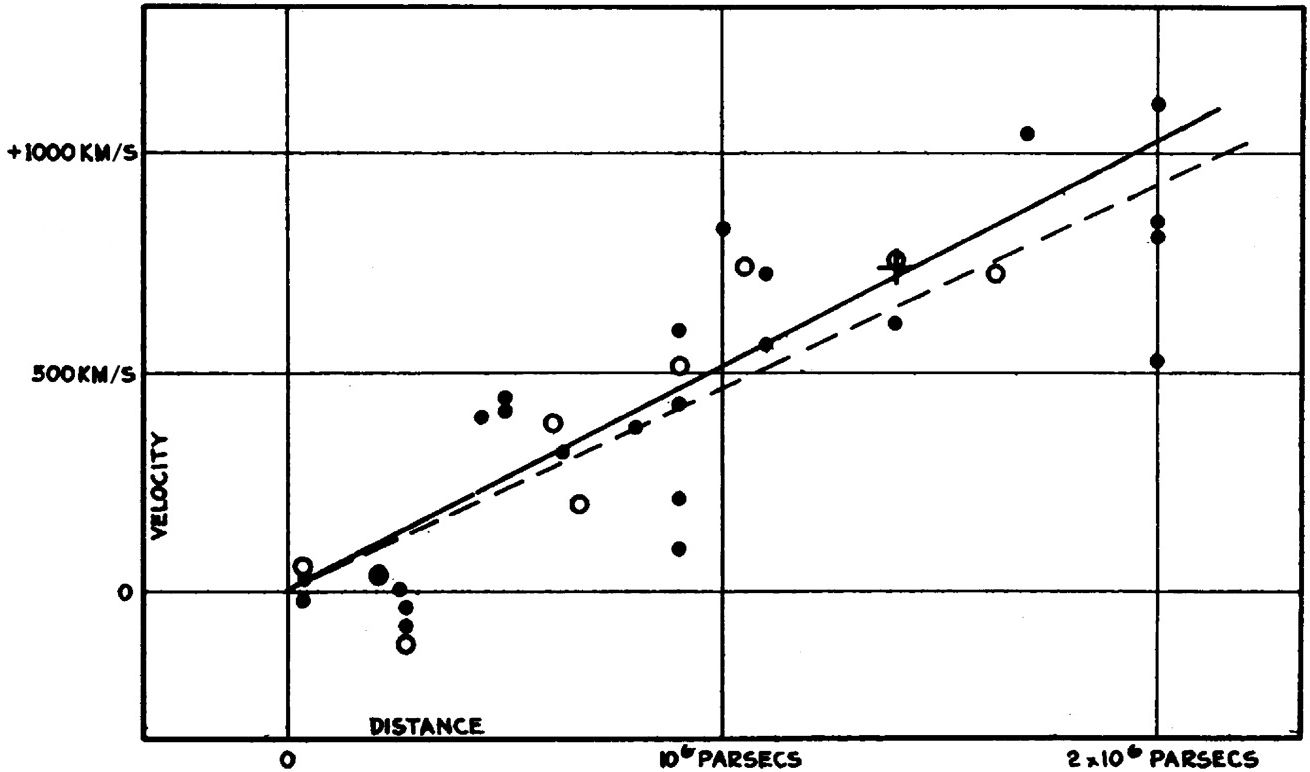
\includegraphics[width=0.8\textwidth]{pnas-168fig.jpeg}

	Edwin Hubble's plot of the velocity-distance relation among galaxies in his original paper
	\vspace*{-12pt}
\end{figure}


this\index{Hubble's law} is known as \keypoint{Hubble's law}\footnote{Edwin Hubble made this conclusion based on his study of 46 galaxies. Later observations further supported the proportional relationship between the recession speed of galaxies and the distance, but the constant computed by Edwin Hubble himself was found to be greatly overestimated. Hubble's original paper can be seen here: \url{https://www.pnas.org/doi/full/10.1073/pnas.15.3.168}}
\begin{equation*}
	\boxed{v = H_0 d} \qquad \text{ Hubble constant: } H_0 \approx 2.4 \times10^{-18} \text{ s}^{-1}
\end{equation*}

\cmt exact value of the Hubble constant is not accurately known

$H_0$ is believed to be between $1.5 \times10^{-18} \text{ s}^{-1} \sim 3.5 \times10^{-18}\text{ s}^{-1}$ (uncertainty around $\pm 40\%$!)


\example{The K-line of inoised calcium from the absorption spectrum of the galaxy NGC 4889 is measured to be 401.8 nm. The same K-line measured in a laboratory setting is known to be 393.3 nm. (a) What is the speed of the NGC 4889? (b) How long does it take for light to reach us from NGC 4889?}

\sol recession speed: $v = \frac{\Delta \lambda}{\lambda} \times c = \frac{401.8-393.3}{393.3}\times 3.00\times10^8 \approx 6.48 \times 10^6 \mps$

distance of galaxy: $d = \frac{v}{H_0} \approx \frac{6.48\times10^6}{2.4\times10^{-18}} \approx 2.7 \times 10^{24} \text{ m}$

time for light to propagate: $t = \frac{d}{c} = \frac{2.7 \times 10^{24}}{3.00\times10^8} \approx 9.0\times10^{15} \text{ s} \approx 2.9\times10^{8} \text{ years}$

\subsubsection{Big Bang theory}\index{Big Bang}

Hubble's law implies the universe is \emph{expanding}

go back in time, all galaxies must be close together

this suggests the universe must begin from a highly dense state

it is now generally accepted that the universe is created from a dramatic explosion

this starting point of the universe and everything is known as the \keypoint{Big Bang}\footnote{The Big Bang Theory was proposed in 1927 by Belgian astronomer and cosmologist \emph{Georges Lemaitre}. From a theoretical view, Lemaitre deduced that the natural consequence of Einstein's theory of general relativity must be an expanding universe. In 1929, \emph{Edwin Hubble}, who was unaware of Lemaitre's work, published his famous relation between distance and radial velocity among extra-galactic nebulae. Nevertheless, Hubble's discovery became a strong supporting evidence for the Big Bang theory.}

\subsubsection*{age of the universe}

age of the universe can be deduced from Hubble's law

consider two galaxies started off close together during the Big Bang

assume galaxies have been moving away from one another at constant speed $v$ for time $t$

distance between the two galaxies today would be $d=vt$

but this $t$ is essentially all the time since beginning of the universe

so age of the universe: $t=\frac{d}{v} = \frac{d}{H_0 d} \RA \boxed{ t= \frac{1}{H_0}}$

substitute $H_0 \approx 2.4 \times10^{-18} \text{ s}^{-1}$, one finds $t\approx 4.5\times10^{18} \text{ s}$, which is about 14 billion years (Gy)

\cmt there is great uncertainty in the universe's age (varying from $11\sim20 \text{ Gy}$)

two main reasons for this uncertainty are:

\begin{compactitem}

\item[--] our calculation is based on the assumption of constant recession speed

there are cosmological models that suggest otherwise, so different ages are predicted 

\item[--] our calculation also depends on the value of $H_0$

but exact value of $H_0$ is in doubt due to large uncertainty in distance measurements

\end{compactitem}


\begin{wrapfigure}{r}{0.52\textwidth}
    \vspace*{-15pt}
    \centering
	\begin{tikzpicture}[scale=0.96]
		\node[rotate=90] at (-1, 3) {velocity / $10^3 \text{ km s}^{-1}$};
		\node at (3, -1) {distance / $10^6$ ly};
		\foreach \y/\ytext in {0/0, 1/2, 2/4, 3/6, 4/8, 5/10, 6/12} \node[left] at (0,\y) {\ytext};
		\foreach \x/\xtext in {0/0, 1/100, 2/200, 3/300, 4/400, 5/500, 6/600} \node[below] at (\x, 0) {\xtext};
		\draw[thin, gray!50, step=0.1] (0,0) grid (6,6);
		\draw[step=0.5] (0,0) grid (6,6);
		\draw plot[mark=*, mark options={fill=white}] (1.20, 0.93);
		\draw plot[mark=*, mark options={fill=white}] (1.42, 1.59);
		\draw plot[mark=*, mark options={fill=white}] (1.64, 2.05);
		\draw plot[mark=*, mark options={fill=white}] (2.60, 2.52);
		\draw plot[mark=*, mark options={fill=white}] (2.85, 3.22);
		\draw plot[mark=*, mark options={fill=white}] (3.40, 4.03);
		\draw plot[mark=*, mark options={fill=white}] (3.62, 3.65);
		\draw plot[mark=*, mark options={fill=white}] (4.27, 3.79);
		\draw plot[mark=*, mark options={fill=white}] (4.43, 4.80);
		\draw plot[mark=*, mark options={fill=white}] (4.45, 4.51);
		\draw plot[mark=*, mark options={fill=white}] (4.91, 5.54);
		\draw plot[mark=*, mark options={fill=white}] (5.51, 5.10);
		\draw plot[mark=*, mark options={fill=white}] (5.76, 5.57);
		\draw[thick, blue] (0,0) -- (5.8, 6);
		\end{tikzpicture}
    \vspace*{-18pt}
\end{wrapfigure}

\question{The plot shows some data on the velocities and distances for a set of galaxies. A fit line has also been drawn. (a) Compute a value for the Hubble constant $H_0$ based on the data given. (b) Estimate the age of the universe using your calculated value for $H_0$, and state any assumption that you make. (c) For a galaxy at a distance of $2\times10^9 \text{ ly}$, what is the fractional change in the wavelength of its spectrum?}



\subsubsection*{cosmic microwave background radiation}\index{comsmic microwave background}

another key evidence for the Big Bang model is the \emph{cosmic microwave background}

after Big Bang, universe gradually cools down due to expansion

the universe today should be filled with radiation due to remnant heat from the Big Bang

theoretical calculation predicts that the universe should now have a temperature of 2.7 K

this suggests a background radiation peaked at around 1 mm (microwave band)

this radiation is therefore called \keypoint{cosmic microwave background} (CMB)\footnote{\emph{Ralph Alpher}, \emph{George Gamow} and \emph{Robert Herman} suggested the idea of CMB in theory in the 1940s. In 1965, \emph{Robert Dicke} took up the problem and led a team of physicists at Princeton University to hunt for the CMB signal. In the same year, \emph{Arno Penzias} and \emph{Robert Wilson} at the Bell Laboratories built a large radio antenna for a communication satellite in New Jersey, while they failed in all attempts to get rid of the `background noise' that came from all directions.

When Princeton's team heard about the Bell Lab's result, they realized at once that the CMB had already been found. As a result, two important articles were published: one by Penzias and Wilson about the `noise', the other by Dicke's team explaining its true nature. Penzias and Wilson did not interpret what they had found in their article, nor did they have any intention to look for CMB in the first place. Nevertheless, they received the Nobel Prize in Physics in 1978, for their accidental discovery of CMB. What about Dicke and his team? Quoting \emph{Bill Bryson's A Short History of Nearly Everything}, the Princeton researchers got only sympathy.}

CMB radiation have been observed by space telescopes from all directions of cosmos\footnote{Three major CMB missions include: (1) the Cosmic Background Explorer (COBE), launched by NASA in 1989, (2) the Wilkinson Microwave Anisotropy Probe (WMAP), launched by NASA in 2001 to study fluctuations in CMB in greater detail, (3) the Planck satellite, launched by ESA in 2009 to study CMB fluctuations with even greater sensitivity. These studies would allow scientists to trace back to what happened immediately after the Big Bang, and the understanding of the early universe is crucial for the understanding of the large-scale cosmic structures that we see today.}

CMB corresponds to a temperature of around 3 K, which is pretty close to the prediction

 \question{Use Wien's law to show that the peak intensity of the electromagnetic radiation given off by a black body at a temperature of 3 K is around 1 mm.}


\subsubsection{fate of the universe ($\ast$)}

whether the universe will expand forever depends on strength of gravity

fate of universe narrows down to how density $\rho$ of universe compares to critical density $\rho_c$

\begin{compactitem}

\item[--] if $\rho > \rho_c$, force of gravity dominates as there is sufficient matter

expansion will slow down, then contract back inwards

this leads to a \emph{closed} universe, eventually ending in a \emph{Big Crunch} 

\item[--] if $\rho < \rho_c$, there is not enough gravity to stop expansion

expansion continues forever, leading to an \emph{open} universe

\end{compactitem}

but the big problem is, it is difficult to determine average density of our universe

\cmt issue of \emph{dark matter}\index{dark matter}

mass of galaxies suggested by luminosity calculation cannot provide the centripetal force needed to keep galaxies rotating

galaxies must contain mass that does not give off light, known as \keypoint{dark matter}

\cmt issue of \emph{dark energy}\index{dark energy}

observation shows expansion of universe is not slowing down

it is suggested that cosmic acceleration is caused by \keypoint{dark energy}

\begin{figure}[ht]
    \centering
	\begin{tikzpicture}
		\draw[thick] (0,0) circle (2);
		\draw[thick] (0,0) -- (68:2);
		\draw[thick] (0,0) -- (165.2:2);
		\draw[thick] (0,0) -- (50:2);
		\draw[thick] (58.8:1.8) --++ (1,0.5) node[right, twolinecap] {ordinary matter\\5\%};
		\draw[thick] (-40:1.7) --++ (1.1,-0.6) node[right, twolinecap] {dark energy\\68\%};
		\draw[thick] (120:1.8) --++ (-1,0.6) node[left, twolinecap] {dark matter\\27\%};
    \end{tikzpicture}
    \vspace*{-12pt}
\end{figure}


\cmt it turns out ordinary matter only contributes to a very small part of the universe

great majority of the total mass-energy content of cosmos is dark matter and dark energy

but nature of dark matter and dark energy are not yet understood
\section{Electronics}

electronic sensors basically consist of three parts

change in some physical property (temperature, pressure, etc.) is picked up by a \keypoint{sensor}

electrical signal is then fed to \keypoint{processing units}

processor produces an output voltage to drive \keypoint{output devices} to indicate this change

\subsection{sensors}

\subsubsection{thermistor}

\begin{wrapfigure}{r}{0.45\textwidth}
	\centering
		\begin{circuitikz}[european resistors]
		\draw[thick] (0,0) to [thR,l_=$R_T$] (3,0);
	\end{circuitikz}
	\caption*{electric symbol for thermistor}
	
	\vspace*{\baselineskip}
	\begin{tikzpicture}[scale=0.8]
	\draw[->] (-1.6,0) -- (5,0) node[below] {$T$/\OC};
	\draw[->] (0,0) node[below]{0} -- (0,4) node[above] {$R_T$};
	\draw[blue,thick] (-1.5,4) [out=-60,in=170] to (4.8,0.8);
	\end{tikzpicture}
\end{wrapfigure}

\keypoint{thermistor}\index{thermistor} is an electrical component with a resistance that varies with temperature

thermistors usually have a \emph{negative temperature coefficient}, or NTC in short,  which means their resistance decreases as temperature rises

in A-Levels, we consider NTC thermistors only

\cmt resistance-temperature relation is \emph{non-linear}
	
if a graph is sketched, the curve looks like an exponential decay
	
\cmt behaviour of NTC thermistors can be explained in terms of \emph{band theory} (see \S\ref{band-theory})

at low temperature, electrons are bound to atoms and cannot move freely; at high temperature, electrons gain energy and break free from atoms, so more free electrons available to conduct electricity

\subsubsection{LDR}

\begin{wrapfigure}{r}{0.4\textwidth}
	\vspace*{-16pt}
	\centering
	\begin{circuitikz}[european resistors]
		\draw[thick,->] (1.6,0.6) -- ++(-.3,-.3);
		\draw[thick,->] (1.8,0.6) -- ++(-.3,-.3);
		\draw[thick] (0,0) to [R,l_=LDR] (3,0);
	\end{circuitikz}
	
	\caption*{electric symbol for LDR}
	
	\vspace*{\baselineskip}
	\begin{tikzpicture}[scale=0.84]
	\draw[->] (0,0) -- (5,0) node[below left] {$I$};
	\draw[->] (0,0) node[below]{0} -- (0,4) node[above] {LDR};
	\draw[blue,thick] (-0,3.6) [out=-75,in=170] to (4.8,0.8);
	\end{tikzpicture}
\end{wrapfigure}

	

\keypoint{light-dependent resistor}, or \keypoint{LDR}\index{LDR}, is an electrical component with a resistance that can change with intensity of light

resistance of LDR decreases as light level increases

\cmt resistance of LDR varies \emph{non-linearly} with intensity

\cmt behaviour of LDR is also explained with \emph{band theory}

bound electrons acquire energy from radiation and become conducting, greater light intensity means more free electrons available

\cmt in dark, typical resistance of LDR $\approx10^5\sim10^7$ $\Omega$

in bright, typical resistance of LDR $\approx10^2\sim10^3$ $\Omega$


\subsubsection{strain gauge}

\begin{wrapfigure}{r}{0.4\textwidth}
	\centering
	\begin{tikzpicture}[scale=0.75,rotate=30]
	\draw[thick,fill=blue!15,rounded corners] (-2,0) rectangle (3.2,2.4);
	\foreach \x in {0.3,0.7,1.1,1.5} \draw[very thick] (0.3,\x) --++ (2.4,0) arc(-90:90:0.1) --++ (-2.4,0) arc (270:90:0.1);
	\draw[very thick] (0.3,1.9) --++ (2.4,0) arc(-90:90:0.1) --++ (-2.4,0);
	\draw[very thick] (0.3,0.3) [out=180, in=0] to (-2,0.6) --++ (-2,0);
	\draw[very thick] (0.3,2.1) [out=180, in=0] to (-2,1.8) --++ (-2,0);
	\draw (-3,0.5) --++ (-.924,-1.6) node[below,twoline]{connection\\leads};
	\draw (1.8,0.2) --++ (-.924,-1.6) node[below,twoline]{metal\\wire};
	\draw (3,2.1) --++ (-1,1.6) node[above,twoline]{plastic\\sheet};
	\end{tikzpicture}
	
	\caption*{structure of a strain gauge}
\end{wrapfigure}

to measure width of a narrow crack, a device called \keypoint{strain gauge}\index{strain gauge} is widely used in industry

a metal-wire strain gauge consists of a folded long wire sealed on a thin plastic box

as crack widens, strain gauge gets stretched, length of wire increases, causing a change in its resistance

resistance of a metal wire is given by: $R=\frac{\rho l}{A}$

increase in resistance is proportional to increase in length of wire (for small increments)

\cmt if change in cross-sectional area of wire is negligible

increase in resistance: $\Delta R = \frac{\rho\Delta l}{A} \ra \boxed{\frac{\Delta R}{R} = \frac{\Delta l}{l}}$

\cmt if cross-sectional area of wire changes with its length

total volume of wire $V=Al$ should remain constant

it can be shown that
\footnote{To keep $V=Al$ constant, for small change in $l$, one has $\frac{\Delta A}{A} \approx \frac{\Delta l}{l}$. Resistance of the stretched wire is: $R+\Delta R = \frac{\rho(l+\Delta l)}{A-\Delta A} = \frac{\rho l}{A} \left(1 + \frac{\Delta l}{l}\right) \left(1 - \frac{\Delta A}{A}\right)^{-1} \approx R \left(1 + \frac{\Delta l}{l}\right) \left(1 - \frac{\Delta l}{l}\right)^{-1}$. For $x\ll1$, we can use binomial expansion $(1+x)^n = 1 + nx + \cdots$. Drop higher order terms, we find to the first-order approximation that: $R+\Delta R \approx R \left(1 + \frac{\Delta l}{l}\right) \left(1 + \frac{\Delta l}{l}\right) \approx R\left( 1 + \frac{2\Delta l}{l}\right)$, so $\Delta R = 2R\frac{\Delta l}{l}$, it then follows that $\frac{\Delta R}{R} = \frac{2\Delta l}{l}$.}
 the percentage increase in resistance is: $\boxed{\frac{\Delta R}{R} = \frac{2\Delta l}{l}}$

notice the differences, change in length causes increase in resistance, reduction in cross section makes the same contribution, hence an extra factor of two.

\subsubsection{piezo-electric transducer}\label{ch-piezo}

\keypoint{piezo-electric transducer}\index{piezo-electric transducer} transforms mechanical energy into electrical energy, or vice versa

when a piezo-electric material\footnote{Materials that exhibit piezo-electricity include quartz, certain ceramics, various proteins, etc.} is compressed, a p.d. is produced across it

conversely, p.d applied across piezo-electric material can cause change in shape

since its discovery, piezo-electricity was exploited in many useful applications



\cmt piezo-electric transducer can be used to generate sound waves

apply an a.c. voltage, material is forced to vibrated at same frequency as a.c.

this causes compression and rarefaction of air, producing sound waves

so piezo-electric transducer is the key component in \emph{loudspeakers} and \emph{buzzers}

\cmt piezo-electric transducer can also be used to detect sound waves

exposed to sounds, variation in air pressure produces an a.c. voltage across the device

this signal can be measured and processed to represent original sound wave

so piezo-electric transducer is also found in \emph{microphones}

\begin{figure}[ht]
	\centering
	\begin{minipage}{0.45\textwidth}
		\centering
		\begin{circuitikz}
			\draw (0,0) to[mic] ++(0,1.8);
		\end{circuitikz}
		\caption*{symbol for a microphone}
	\end{minipage}
	\begin{minipage}{0.45\textwidth}
		\centering
		\begin{circuitikz}
			\draw (0,0) to[loudspeaker] ++(0,-1.8);
		\end{circuitikz}
		\caption*{symbol for a loudspeaker}
	\end{minipage}
\end{figure}

\cmt mechanism of piezo-electricity is explained on molecular level
	
piezo-electric materials consist of \emph{polarised} molecules, also called \emph{dipoles}
	
when being compressed, dipoles rearrange themselves, causing variation of charge density, so small voltage is generated (see illustration)
	
\begin{figure}[ht]
	\vspace*{-10pt}
	\centering
	\includegraphics[height=160pt]{piezo-electric.pdf}
		%\caption{nature of piezo-electricity due to dipole structure}
	\vspace*{-10pt}
\end{figure}
	




\subsection{processors}

\subsubsection{potential divider}

sensors such as thermistor and LDR only produce changes in resistance, but output devices are driven by voltages $\longrightarrow$ \keypoint{potential divider} circuit can be used\index{potential divider}

a potential divider consists of two resistors in series connected to a fixed voltage supply

\begin{wrapfigure}{r}{0.32\textwidth}
	\vspace{-15pt}
	\centering
	\begin{center}
		\begin{circuitikz}[european resistors,yscale=.8,xscale=1.1]
			\draw[thick] (0,5) -- (2,5) to [R,l_=$R_1$] (2,2.5) to [R,l_=$R_2$] (2,0) -- (1,0) node[ground]{} -- (0,0);
			\draw[thick,->] (0.5,0) -- (0.5,5) node[left,midway]{$V_0$};
			\foreach \h in {0,2.5,5} \draw[thick] (2,\h) -- ++(1,0);
			\draw[thick,<->] (2.7,2.5) -- ++ (0,2.5) node[midway,right]{$V_1$};
			\draw[thick,<->] (2.7,0) -- ++ (0,2.5) node[midway,right]{$V_2$};
			\node[left] at (2,2.5) {$X$};
		\end{circuitikz}
	\end{center}
	\vspace{-15pt}
\end{wrapfigure}

voltage is shared between the resistors: $V_0 = V_1 + V_2$

p.d. across each resistor: $V_1 = IR_1$, $V_2 = IR_2$

but same current $I$ flows through $R_1$ and $R_2$, so $\boxed{\frac{V_1}{V_2} = \frac{R_1}{R_2}}$

this shows voltage is shared in proportion to resistance

for each resistor: $\boxed{V_1 = \frac{R_1}{R_1+R_2}V_0}, \, \boxed{V_2 = \frac{R_2}{R_1+R_2}V_0}$

\cmt if $R_1$ increases, while $R_2$ is fixed, then $V_1\up$, $V_2 \down$

if $R_1$ decreases, while $R_2$ is fixed, then $V_1\down$, $V_2 \up$

\cmt sometimes we need specify \emph{electric potential} at a given point

potential at any point is measured with respect to a reference point

this point is called \keypoint{earth} or \keypoint{ground}, with a potential defined to be zero

for example, potential at $X$ is essentially equal to voltage $V_2$



\begin{wrapfigure}{r}{0.35\textwidth}
	\vspace{-10pt}
	\centering
	\begin{circuitikz}[european resistors,yscale=1.2]
		\draw[thick,->] (0.58,1.1) -- ++(-.3,-.3);
		\draw[thick,->] (0.58,1.3) -- ++(-.3,-.3);
		\draw[thick] (-2,4)node[left] {$+V_0$} -- (0,4) to [R,l_=$R_0$] (0,2) to [R,l_=LDR] (0,0) -- (-1,0) node[ground]{} -- (-2,0);
		\draw[thick] (0,0) -- (2,0);
		\draw[thick] (0,2) -- (2,2);
		\draw[thick,<->] (1.5,0) -- (1.5,2) node[midway,right]{$V_\text{out}$};
	\end{circuitikz}
\end{wrapfigure}

\example{For the sensing circuit shown, suggest how the output voltage changes as light level increases.}\label{ex-light-sensor}

\sol intensity of light increases, resistance of LDR decreases

current in circuit increases, p.d. across $R_0$ increases

so p.d. across LDR becomes smaller, $V_\text{out}$ would decrease

from $V_\text{out} = \frac{\text{LDR}}{\text{LDR} + R_0}V_0$, one can also see $V_\text{out}$ decreases when resistance of LDR becomes lower

so $V_\text{out}$ decreases as light intensity increases \eoe

\question{In Example \ref{ex-light-sensor}, if the fixed resistor has $R_0 = 8.0$ k$\Omega$, and the LDR is in an environment such that it has a resistance of $12$ k$\Omega$. The voltage supply $V_0 = +15 \text{ V}$. Find $V_\text{out}$.}

\question{Design a sensing circuit that produces a greater output voltage as the temperature of the sensor rises. Explain the operation of your circuit.}


\subsubsection{op-amp: basics}

to amplify small input into large output signals, we need \keypoint{operational amplifiers (op-amp)}\index{amplifier!op-amp}\footnote{We are not concerned with what is inside an operational amplifier. An op-amp contains several \emph{transistors}, and you are not required to know how they work in the A-Level syllabus. You only need to know what output voltage an op-amp would produce to drive output devices. If you want to learn more details on the functions of op-amps, you need to study a higher level course on \emph{Electronics}.}

\begin{wrapfigure}{R}{0.35\textwidth}
	\vspace{-15pt}
	\centering
	\begin{circuitikz}[european resistors]
		\draw[thick] (0,0) node[op amp] (opamp) {}
		(opamp.+) --++ (-.8,0) node[left]{$V_+$}
		(opamp.-) --++ (-.8,0) node[left]{$V_-$}
		(opamp.out) --++ (.8,0) node[above]{$V_\text{out}$}
		(opamp.down) -- ++ (0,-.8) node[right] {$-V_S$}
		(opamp.up) -- ++ (0,.8) node[right] {$+V_S$};
	\end{circuitikz}
	\caption*{circuit symbol for op-amp}
	\vspace{-15pt}
\end{wrapfigure}


op-amp is building block for many electronic devices

\cmt an op-amp has several terminals:

\begin{compactitem}
	\item[--] $V_+$: non-inverting input
	
	\item[--] $V_-$: inverting input
	
	\item[--] $\pm V_S$: positive/negative power supply voltages
	
	\item[--] $V_\text{out}$: output voltage
\end{compactitem}

\cmt output voltage of op-amp is given by: $\boxed{V_\text{out}= G_0(V_+ - V_-)}$

$G_0$ is value of amplification of an open-loop\footnote{It is called an open loop in the sense that there is no loop linking $V_\text{out}$ to input terminals of the op-amp.} amplifier, called \keypoint{open-loop gain}

\cmt value of $G_0$ is not well controlled in manufacturing processes

$G_0$ may also depend on temperature of op-amp, frequency of input signals, etc.

\cmt output voltage of op-amp cannot exceed supply voltages

when $V_\text{out}$ calculated is greater than $V_S$, the op-amp becomes \keypoint{saturated}, true $V_\text{out}$ of op-amp is close to $+V_S$ or $-V_S$ depending on polarity of $V_\text{out}$

\cmt all voltages in amplifier circuits are measured with respect to a reference level set at \emph{earth}

\subsubsection*{properties of ideal op-amps}

an ideal op-amp is considered to have the following properties

\begin{itemize}[leftmargin=\parindent]
	\item[$\circ$] \emph{infinite open-loop gain} ($G_0 \to \infty$)
	
	want large $V_\text{out}$ for small $V_\text{in}$, value of amplification should be as large as possible\footnote{Open-loop gain of an actual op-amp: $G_0 \approx 10^5 \sim 10^7$.}
	
	\item[$\circ$] \emph{infinite input resistance/impedance}\footnote{Impedance is an extension of the concept of resistance to a.c. circuits. You might just think of impedance of an electrical component as its ability to oppose currents.}
	
	want $V_\text{in}$ to op-amp to be as large as possible
	
	so large resistance between input terminals of op-amp\footnote{Typical input impedance of an actual op-amp: $10^6$ $\Omega$ or higher.}
	
	a consequence is that (almost) no current flows into or leaves the input terminals
		
	
	\item[$\circ$] \emph{zero output resistance/impedance}
	
	output impedance of op-amp acts like internal resistance of batteries
	
	want largest possible $V_\text{out}$ to load, so small resistance for output terminal\footnote{Typical output impedance of an actual op-amp: $10^1\sim10^2$ $\Omega$.}
	
	\item[$\circ$] \emph{infinite bandwidth}
	
	\keypoint{bandwidth} refers to range of frequencies of input voltages that are amplified by same amount
	
	want same gain for all input frequencies, so infinite bandwidth is desired
	
	\item[$\circ$] \emph{infinite slew rate}: $V_\text{out}$ changes immediately with $V_\text{in}$, response is instantaneous
	
	\item[$\circ$] \emph{zero noise}: $V_\text{out}$ does not change with disturbance due to external conditions
\end{itemize}

\subsubsection{voltage comparator}

for an open-loop op-amp, since gain $G_0$ is very large, so as long as there is a small difference in $V_+$ and $V_-$, $V_\text{out} = G_0 (V_+ - V_-) \to \pm \infty$, this causes $V_\text{out}$ to saturate

so $V_\text{out} = \pm V_S$ depending on which one of $V_+$ and $V_-$ is larger, this makes a comparator\index{voltage comparator}\index{amplifier!comparator}

\begin{ilight}
	a \keypoint{voltage comparator} compares two input voltages $V_+$ and  $V_-$, and produces a $V_\text{out}$ to indicate which one is greater: if $V_+ > V_-$, then $V_\text{out} = +V_S$; if $V_+ < V_-$, then $V_\text{out} = -V_S$
\end{ilight}

\example{A circuit that incorporates an ideal op-amp is shown. Given that $R_0 = 10\text{ k}\Omega$, variable resistor is set to $R = 20\text{ k}\Omega$, and the thermistor has a resistance of $R_T = 40\text{ k}\Omega$ at 20\OC, and $R_T = 10\text{ k}\Omega$ at 50\OC. Describe the change in $V_\text{out}$ as temperature rises from 20$^\circ$C to 50$^\circ$C.}

\begin{figure}[ht]
	\centering
		\begin{circuitikz}[european resistors,scale=1]
			\draw[thick] (2,3) node[right] {$+9\text{V}$} -- (-6,3);
			\draw[thick] (-6,-3) to [thR,l^=$R_T$] (-6,-.5) -- (-6,.5) to [vR,l^=$R$] (-6,3);
			\draw[thick] (-6,-3) -- ++ (7,0)node[ground]{} -- ++(1.5,0);
			\draw[thick] (-3.5,3) to [R,l_=$R_0$] (-3.5,.5) -- ++(0,-1) to [R,l_=$R_0$] ++(0,-2.5);
			\draw[thick] (0,0) node[op amp] (opamp) {}
			(opamp.+) -- (-3.4,-0.5) arc(0:180:0.1) -- (-6,-.5) node[above right]{$A$}
			(opamp.-) -- (-3.5,.5) node[above right]{$B$}
			(opamp.out) -- (2.5,0)
			(opamp.down) -- ++ (0,-.8) node[right] {$-9\text{V}$}
			(opamp.up) -- (0,3);
			\draw[<->,thick] (2,0) -- (2,-3) node[midway,right]{$V_\text{out}$};
		\end{circuitikz}
\end{figure}
	
\sol this is a comparator whose input voltages are determined from two potential divider circuits

resistor $R_0$ sets a constant potential for reference: $V_- = V_B = \frac{10}{10+10}\times (+9) = +4.5\text{ V}$
	
p.d. across $R_T$ determines $V_A$, which is fed into $V_+$ to be compared with $V_-$
	
at 20\OC: $V_+ = V_A = \frac{40}{40+20}\times (+9) = +6.0 \text{ V}$, so $V_+>V_- \ra V_\text{out} = +9\text{ V}$
	
\eqyskip at 50\OC, $V_+ = V_A = \frac{10}{10+20}\times (+9) = +3.0 \text{ V}$, so $V_+ < V_- \ra V_\text{out} = -9\text{ V}$
	
as temperature goes from 20$^\circ$C to 50$^\circ$C, $V_\text{out}$ initially maintains at $+9$ V

it switches over to $-9$ V at some critical temperature then stays at $-9$ V until 50$^\circ$C \eoe

\newpage

\example{The diagram shows a circuit incorporating an ideal op-amp. The variation with time for input voltage $V_\text{in}$ is shown. Sketch the variation of the output voltage.}

\begin{figure}[ht]
	\begin{minipage}{0.45\textwidth}
		\centering
		\begin{circuitikz}[european resistors]
		\draw[thick] (0,0) node[op amp] (opamp) {}
		(opamp.+) -- (-2,-0.5)
		(opamp.-) -- (-1.9,0.5) arc(0:180:0.1) -- (-3.5,0.5) node[left]{$V_\text{in}$}
		(opamp.out) -- (2,0)
		(opamp.down) -- ++ (0,-.8) node[right] {$-9$V}
		(opamp.up) --++ (0,.8) node[right]{$+9$V};
		\draw[<->,thick] (1.6,0) -- (1.6,-2.5) node[midway,right]{$V_\text{out}$};
		\draw[thick] (-3,-2.5) -- (1,-2.5) node[ground]{} -- (2,-2.5);
		\draw (-2,-2.5) to[R,l^=4.0k$\Omega$] (-2,-0.5) -- (-2,0.5) to[R,l^=6.0k$\Omega$] (-2,2.5) -- (-3.5,2.5) node[left]{+5V};
		\end{circuitikz}
	\end{minipage}\hfil
	\begin{minipage}{0.48\textwidth}
		\centering
		\begin{tikzpicture}
		\draw[->] (0,-2.5) -- (0,3) node[left]{$V$/V};
		\draw[->] (0,0) -- (5.75,0) node[right]{$t$/ms};
		\draw[step=0.5, gray, very thin] (0,-2.5) grid (5.5,2.5);
		\foreach \x in {0,10,...,50} {
			\draw[white,fill] (\x/10-0.2,-0.42) rectangle (\x/10+0.2,-0.08);
			\node[below] at (\x/10,0) {$\x$};
		}
		\foreach \y in {-10,-8,...,10} \node[left] at (0,\y/4) {$\y$};
		\draw [very thick,blue,domain=0:5.5,samples=36,smooth,variable=\x] plot (\x,{0.5+(\x-1.5)*(\x-3.5)*(\x-5)*exp(-0.15*(\x-3.5)*(\x-3))*0.2}) node[right]{$V_\text{in}$};
		\draw[very thick,red] (0,2.25) --++ (1.5,0) --++ (0,-4.5) --++ (2,0) --++ (0,4.5) -- (5,2.25) --++ (0,-4.5) -- (5.5,-2.25) node[right]{$V_\text{out}$};
		\end{tikzpicture}
	\end{minipage}
\end{figure}
	
\sol potential at non-inverting input: $V_+ = \frac{4.0}{4.0+6.0}\times(+5) = +2\text{ V}$

potential at inverting input is equal to input voltage: $V_-=V_\text{in}$

for $V_\text{in}$ greater than +2 V, $V_->V_+$, then $V_\text{out}=-9\text{ V}$

for $V_\text{in}$ less than +2 V, $V_-<V_+$, then $V_\text{out}=+9\text{ V}$

variation of $V_\text{out}$ can then be plotted, which shows the form of a square wave \eoe

\subsubsection{negative feedback}

in practical uses, we may desire $V_\text{out}$ to reflect small changes in $V_\text{in}$, instead of stuck at $\pm V_S$

there are a few problems with open-loop amplifiers that we need to deal with:

\begin{compactitem}
	\item[--] gain of amplifier is too high
	
	$V_\text{out}$ almost always saturates, so $V_\text{out}$ cannot change continuously with $V_\text{in}$
	
	\item[--] open-loop gain $G_0$ of practical op-amp is affected by temperature
	
	different $V_\text{out}$ for the same $V_\text{in}$ at different temperatures is not convenient
	
	\item[--] open-loop gain $G_0$ is a function of input frequency
	
	different input frequencies are not always amplified by same amount
	
	this would cause distortion of original signal, bandwidth would be limited
\end{compactitem}






one way to improve properties of amplifier circuits is to introduce negative feedback

feedback means sending a portion of output voltage back to the input terminals

a feedback network is also called a \emph{closed loop}

\begin{ilight}
	if a fraction of output $V_\text{out}$ is sent back to inverting input $V_-$ such that it opposes changes of input, this is called \keypoint{negative feedback}\index{negative feedback}\index{amplifier!negative feedback}
\end{ilight}

\begin{figure}[ht]
	\centering
	\begin{circuitikz}[european resistors]
		\draw[thick] (0,0) node[op amp] (opamp) {}
		(opamp.+) -- (-3.2,-0.5) node[left]{$V_+$}
		(opamp.-) -- (-2,0.5) -- (-2,2) -- (2,2) -- (2,0) (-2,0.5) -- (-3.2,0.5) node[left]{$V_-$}
		(opamp.out) -- (3,0) node[right]{$V_\text{out}$}
		(opamp.down) -- ++ (0,-.6) node[right] {$-V_S$}
		(opamp.up) -- ++ (0,.6) node[right] {$+V_S$};
		\draw[thick,blue,->] (1,2.4) [out=170,in=10] to (-1,2.4) ; 
		\node[blue,above] at (0,2.5) {$\beta V_\text{out}$};
	\end{circuitikz}

\caption*{negative feedback mechanism}
\end{figure}

let's look into the effect of introducing negative feedback into the amplifier circuit\footnote{Discussions in this section are not required by the syllabus. If you do not have the appetite, you may just skip to the conclusions.}

assume a fraction of output $\beta V_\text{out}$ ($0 < \beta \leq 1$) is fed back to inverting input of op-amp, then combined voltage to this terminal would be the sum of original $V_-$ and the feedback $\beta V_\text{out}$, the equation $V_\text{out} = G_0(V_+-V_-)$ for open-loop circuit shall be rewritten, hence we have



{
	
\centering
	
$V_\text{out} = G_0 \Big[( V_+ - (V_- + \beta V_\text{out})\Big]
\RA (1+G_0\beta)V_\text{out} = G_0(V_+ - V_-)
\RA V_\text{out} = \frac{G_0}{1+G_0\beta }(V_+ - V_-)$
	
}

overall gain of negative feedback amplifier is: $G=\frac{G_0}{1+ G_0\beta}$

this gain is less than open-loop gain $G_0$, so gain is reduced

further notice that $G_0\beta \gg 1$, we find $G \approx \frac{G_0}{\beta G_0} = \frac{1}{\beta}$

this shows for negative-feedback amplifier, as long as open-loop gain $G_0$ is sufficiently large, overall gain $G$ depends on $\beta$ only, i.e., only depends on how much output is sent back to $V_-$


$\beta$ can be controlled by a set of fixed resistors, which are not sensitive to change of frequency or temperature, so $G$ remains constant for a wider range of frequencies and temperatures




\newpage

we conclude that introducing negative feedback has the following benefits:

\begin{itemize}[leftmargin=\parindent]
	\item[$\circ$] reduced gain
	
	\item[$\circ$] more stable gain
	
	\item[$\circ$] increased bandwidth
	
	\item[$\circ$] less distortion
\end{itemize}


\subsubsection*{the golden rule}

with negative feedback, we expect that $V_\text{out}$ is able to change correspondingly with $V_\text{in}$

for any op-amp, $V_\text{out} = G_0(V_+-V_-)$, but op-amp has very large open-loop gain $G_0$

if $V_\text{out}$ does not saturate, one must have $V_+ - V_- \approx 0$

this can be summarised as the \emph{golden rule}: output of op-amp attempts to do whatever is necessary to make the difference between the two input voltages zero

note that op-amp can do this only if there is negative feedback

\subsubsection{inverting amplifier}

one type of widely-used amplifier circuit is called \keypoint{inverting amplifier}\index{amplifier!inverting amplifier}

\begin{figure}[htp]
\centering
\begin{circuitikz}[european resistors,scale=1.25]
	\draw[thick] (0,0) node[op amp] (opamp) {}
	(opamp.+) -- (-2,-0.4) -- (-2,-1.6) node[ground]{} 
	(opamp.-) -- (-2,0.4) to [R,l_=$R_\text{in}$] (-5,0.4) node[left]{$V_\text{in}$}
	(opamp.out) -- (3,0) node[right]{$V_\text{out}$}
	(opamp.down) -- ++ (0,-.6) node[right] {$-V_S$}
	(opamp.up) -- ++ (0,.6) node[right] {$+V_S$};
	\draw[thick] (2,0) -- (2,2) to[R,l_=$R_\text{f}$] (-2,2) -- (-2,0.4);
	\draw[-triangle 60] (-2.5,0.4) -- ++(.1,0) node[below]{$I_\text{in}$};
	\draw[-triangle 60] (-1.4,0.4) -- ++(.1,0) node[below]{$i$};
	\draw[-triangle 60] (-2,1.2) -- ++(0,.1) node[right]{$I_\text{f}$};
\end{circuitikz}
	
\caption*{inverting amplifier}
\end{figure}

$V_\text{out}$ is related to $V_\text{in}$ by $\boxed{V_\text{out} = \left(-\frac{R_\text{f}}{R_\text{in}}\right)V_\text{in} }$, where gain of the amplifier is $G=\frac{V_\text{out}}{V_\text{in}} = -\frac{R_\text{f}}{R_\text{in}}$
	
to show this relation, we need two approximations

\cmt virtual earth approximation: if $V_\text{out}$ does not saturate, must have $V_+ \approx V_-$, but $V_+$ is earthed, i.e., $V_+=0$, so $V_-\approx 0$, referred to as a \keypoint{virtual earth}

\cmt small current approximation: because of the very large input impedance of op-amp, current flowing into inverting input is negligible, i.e., $i\approx 0$

therefore currents through $R_\text{in}$ and $R_\text{f}$ are approximately the same: $I_\text{in} = I_\text{f}$

from this equation, we can relate $V_\text{out}$ to $V_\text{in}$:

{
	\centering
	
	$\frac{V_\text{in} - V_-}{R_\text{in}} = \frac{V_- - V_\text{out}}{R_\text{f}}
	\RA \frac{V_\text{in}-0}{R_\text{in}} = \frac{0-V_\text{out}}{R_\text{f}} 
	\RA V_\text{out} = \left(-\frac{R_\text{f}}{R_\text{in}}\right)V_\text{in}$
		
}

\subsubsection{non-inverting amplifier}

another type of common amplifier circuit is called \keypoint{non-inverting amplifier}\index{amplifier!non-inverting}

\begin{figure}[htp]
	\centering
	\begin{circuitikz}[european resistors,scale=1.25]
		\draw[thick] (0,0) node[op amp] (opamp) {}
		(opamp.+) -- (-1.9,-0.4) arc (0:180:0.1) -- (-3.6,-0.4) node[left]{$V_\text{in}$}
		(opamp.-) -- (-2,0.4) -- (-2,-1.6) to [R,l_=$R_\text{f}$] (2,-1.6) -- (2,0)
		(opamp.out) -- (3,0) node[right]{$V_\text{out}$}
		(opamp.down) -- ++ (0,-.6) node[right] {$-V_S$}
		(opamp.up) -- ++ (0,.6) node[right] {$+V_S$};
		\draw[thick] (-2,-1.6) -- (-2,-2.4) to[R,l_=$R_0$] (-2,-4) node[ground]{} ;
		\draw[-triangle 60] (-1.2,-1.6) -- ++(-.1,0) node[below]{$I_\text{f}$};
		\draw[-triangle 60] (-2,-2.2) -- ++(0,-.1) node[left]{$I_0$};
		\draw[-triangle 60] (-2,-1) -- ++(0,.1) node[left]{$i$};
	\end{circuitikz}
	
	\caption*{non-inverting amplifier}
\end{figure}

for this circuit, $V_\text{out}$ is given by: $\boxed{V_\text{out} = \left(1 + \frac{R_\text{f}}{R_0}\right)V_\text{in}}$, where overall gain $G=\frac{V_\text{out}}{V_\text{in}} = 1 + \frac{R_\text{f}}{R_0}$

to show this, recall current into input of op-amp $i\approx0$ due to its large input impedance, so

{

\centering
	
$I_\text{0} = I_\text{f} \RA \frac{V_- - 0}{R_0} = \frac{V_\text{out} - V_- -}{R_\text{f}}$

}


again, if $V_\text{out}$ is not saturated, $V_- \approx V_+ = V_\text{in}$, then we find


{
	
\centering

$\frac{V_\text{in}}{R_0} = \frac{V_\text{out} - V_\text{in}}{R_\text{f}} \RA  R_0 V_\text{out} - R_0 V_\text{in} = R_\text{f} V_\text{in}
\RA  V_\text{out} = \left(1 + \frac{R_\text{f}}{R_0}\right)V_\text{in}$
	
}

\subsubsection*{remarks on inverting \& non-inverting amplifiers}

inverting and non-inverting amplifiers are starting point for more complex circuits

before going through detailed examples, let's briefly comment on the results we have found
\begin{equation*}
	\text{for inverting amplifer: } G=\frac{-R_\text{f}}{R_\text{in}} \qquad \text{for non-inverting amplifer: } G=1+\frac{R_\text{f}}{R_0}
\end{equation*}

\cmt circuit's overall gain for both amplifiers only depend on choice of resistors

so gain can now be easily tuned, circuit design becomes more convenient

\cmt no parameter of op-amp shows up in final expressions for overall gain

gain is determined by feedback network, rather than by op-amp's characteristics
	
since value of resistors does not change significantly with temperature or frequency

this again means gain becomes now more stable with negative feedback
	
\cmt for inverting amplifiers, $G<0$, $V_\text{in}$ and $V_\text{out}$ always out of phase (opposite signs)
	
for non-inverting amplifiers, $G>0$, $V_\text{in}$ and $V_\text{out}$ always in phase (same sign)

\cmt the proportional relation between $V_\text{in}$ and $V_\text{out}$ only holds if op-amp is not saturated

if we find $V_\text{out}$ greater than supply voltage from a calculation, true $V_\text{out}$ equals $\pm V_S$



\example{In the inverting amplifier circuit below, $R_1=10$ k$\Omega$, $R_2=50$ k$\Omega$. (a) Find $V_\text{out}$ when $V_\text{in} = +1.0$ V. (b) Find $V_\text{out}$ when $V_\text{in} = -4.0$ V.}

\begin{figure}[ht]
	\centering
	\begin{circuitikz}[european resistors]
		\draw[thick] (0,0) node[op amp] (opamp) {}
		(opamp.+) -- (-2,-0.5) -- (-2,-1.5) node[ground]{} 
		(opamp.-) -- (-2,0.5) to [R,l_=$R_1$] (-5,0.5) node[left]{$V_\text{in}$}
		(opamp.out) -- (3,0) node[right]{$V_\text{out}$}
		(opamp.down) -- ++ (0,-.5) node[right] {$-10$V}
		(opamp.up) -- ++ (0,.5) node[right] {$+10$V};
		\draw[thick] (2,0) -- (2,2) to[R,l_=$R_2$] (-2,2) -- (-2,0.5);
	\end{circuitikz}
\end{figure}

\sol overall gain of the amplifier: $G=-\frac{R_2}{R_1} = -\frac{50\text{k}}{10\text{k}}=-5.0$

for $V_\text{in} = +1.0$ V: $V_\text{out}=(-5.0)\times(+1.0)=-5.0 \text{ V}$

for $V_\text{in} = -4.0$ V: $V_\text{out}=(-5.0)\times(-4.0)=+20 \text{ V}$, output becomes saturated, so $V_\text{out}=+10 \text{ V}$ \eoe


\newpage

\example{In the non-inverting amplifier circuit below, $R_1=48$ k$\Omega$, $R_2=6.0$ k$\Omega$. (a) Find $V_\text{out}$ when $V_\text{in} = +0.5$ V. (b) Find $V_\text{out}$ when $V_\text{in} = -3.0$ V.}

\begin{figure}[ht]
	\centering
	\begin{circuitikz}[european resistors,scale=1]
		\draw[thick] (0,0) node[op amp] (opamp) {}
		(opamp.+) -- (-1.9,-0.5) arc(0:180:0.1) -- (-3.6,-0.5) node[left]{$V_\text{in}$}
		(opamp.-) -- (-2,0.5) -- (-2,-1.6) to [R,l_=$R_1$] (2,-1.6) -- (2,0)
		(opamp.out) -- (3,0) node[right]{$V_\text{out}$}
		(opamp.down) -- ++ (0,-.5) node[right] {$-10$V}
		(opamp.up) -- ++ (0,.5) node[right] {$+10$V};
		\draw[thick] (-2,-1.6) -- (-2,-2.1) to[R,l_=$R_2$] (-2,-4) node[ground]{} ;
	\end{circuitikz}
\end{figure}

\sol overall gain of the amplifier: $G=1+\frac{R_1}{R_2} = 1+\frac{48\text{k}}{6.0\text{k}}=9.0$

for $V_\text{in} = +0.5$ V: $V_\text{out}=9.0\times(+0.5)=+4.5 \text{ V}$

for $V_\text{in} = -3.0$ V: $V_\text{out}=9.0\times(-3.0)=-27 \text{ V}$, output becomes saturated, so $V_\text{out}=-10 \text{ V}$ \eoe


\example{An amplifier circuit incorporating an ideal op-amp is shown.}

\begin{figure}[ht]
	\centering
	\begin{circuitikz}[european resistors,scale=1]
		\draw[thick] (0,0) node[op amp] (opamp) {}
		(opamp.+) -- (-2,-0.5) -- (-2,-2) node[ground]{} 
		(opamp.-) -- (-2,0.5) to [R,l_=$2.0\,k\Omega$] (-6,0.5) 
		(opamp.out) -- (3,0) node[right]{$V_\text{out}$}
		(opamp.down) -- ++ (0,-.6) node[right] {$-8\text{V}$}
		(opamp.up) -- ++ (0,.6) node[right] {$+8\text{V}$};
		\draw[thick] (2,0) -- (2,2) to[R,l_=$20\,k\Omega$] (-2,2) -- (-2,0.5);
		\draw[thick] (3,-2) -- (-6,-2) to [battery, l_=$1.0\text{V}$] (-6,0.5) ;
		\draw[->] (2.8, -2) --++(0,2);
		\draw[thick] (-2,2) -- (-2,3.6) to [thR,l=$R_T$] (2,3.6) -- (2,2);
	\end{circuitikz}
\end{figure}

Initially, the thermistor has a resistance of $20\,k\Omega$. (a) Find the gain of this circuit. (b) Find the output voltage. (c) State and explain how $V_\text{out}$ changes as temperature rises. (d) The thermistor is then removed, find the new output voltage.

\newpage

\solc \begin{compactitem}
	\item[(a)] this is an inverting amplifier (there is negative feedback loop and $V_\text{out}$ is fed into $V_-$)
	
	resistance of feedback loop: $R_\text{f} = \left(\frac{1}{20\text{k}} + \frac{1}{20\text{k}}\right)^{-1} = 10 \, \text{k}\Omega$
	
	\eqyskip gain of amplifer: $G= - \frac{R_\text{f}}{R_\text{in}} = -\frac{10\text{k}}{2.0\text{k}} \RA G=-5.0$
	
	\item[(b)] $V_\text{in}$ is at negative terminal of the battery, which is 1.0 V lower than the positive terminal
	
	but positive terminal is earthed, so $V_\text{in} = -1.0 \text{ V}$
	
	output voltage: $V_\text{out} = GV_\text{in} = (-5.0) \times (-1.0) \RA V_\text{out} = +5.0 \text{ V}$
	
	\item[(c)] as temperature increases, resistance of thermistor decreases
	
	total resistance of feedback loop becomes smaller
	
	gain of the circuit then becomes less negative, so $V_\text{out}$ will decrease
	
	\item[(d)] gain of amplifier after removal of thermistor: $G' = - \frac{R'_\text{f}}{R_\text{in}} = - \frac{20\text{k}}{2.0\text{k}} \RA G' = -10$
	
	new output voltage can be computed: $V'_\text{out} = G'V_\text{in} = (-10)\times(-1.0) = +10 \text{ V}$
	
	but voltage supply to op-amp is $\pm 8 \text{ V}$, op-amp saturates, so $V'_\text{out} = +8 \text{ V}$ \eoe
\end{compactitem}

\example{A circuit incorporating an ideal op-amp is shown below. The two fixed resistors have $R_1=36$ k$\Omega$ and $R_2=9.0$ k$\Omega$. Variation of $V_\text{in}$ from a voltage source is shown with the blue curve. On the same graph, plot how $V_\text{out}$ varies with time.}

\begin{figure}[ht]
	\begin{minipage}{0.52\textwidth}
		\centering
		\begin{circuitikz}[european resistors,scale=1]
			\draw[thick] (0,0) node[plain amp] (opamp) {}
			(opamp.-) -- (-2,0.5) -- (-3.5,0.5) to [sV] (-3.5,-4) -- (3,-4) 
			(opamp.+) -- (-2,-0.5) -- (-2,-1.8) to [R] (1.8,-1.8) -- (1.8,0)
			(opamp.out) -- (3,0)
			(opamp.down) -- ++ (0,-.6) node[right] {$-12$V}
			(opamp.up) -- ++ (0,.6) node[right] {$+12$V};
			\node at (-0.6,0.5) {$+$};
			\node at (-0.6,-0.5) {$-$};
			\draw[->] (2.7,-4) -- (2.7,0) node[midway, right]{$V_\text{out}$};
			\draw[thick] (-2,-1.6) -- (-2,-2.1) to[R,l^=$R_2$] (-2,-4) node[ground]{};
			\node at (0,-2.4) {$R_1$};
		\end{circuitikz}
	\end{minipage}\hfil
	\begin{minipage}{0.45\textwidth}
		\centering
		\begin{tikzpicture}
		\draw[->] (0,-2.5) -- (0,3) node[left]{$V$/V};
		\draw[->] (0,0) -- (5,0) node[below]{$t$/ms};
		\draw[step=0.5, gray, very thin] (0,-2.5) grid (4.5,2.5);
		\foreach \x in {0,10,...,40} {
			\draw[white,fill] (\x/10-0.2,-0.42) rectangle (\x/10+0.2,-0.08);
			\node[below] at (\x/10,0) {$\x$};
		}
		\foreach \y in {-20,-16,...,20} \node[left] at (0,\y/8) {$\y$};
		\draw [very thick,blue,domain=0:4.5,samples=30,smooth,variable=\x] plot (\x,{sin(\x*90)/2}) node[right]{$V_\text{in}$};
		\draw [very thick,red,dotted,domain=0:4.5,samples=30,smooth,variable=\x] plot (\x,{sin(\x*90)*2.5});
		\draw [very thick,red,domain=0:0.4097,samples=10,smooth,variable=\x] plot (\x,{sin(\x*90)*2.5});
		\draw [very thick,red,domain=1.5903:2.4097,samples=10,smooth,variable=\x] plot (\x,{sin(\x*90)*2.5});
		\draw [very thick,red,domain=3.5903:4.4097,samples=10,smooth,variable=\x] plot (\x,{sin(\x*90)*2.5});
		\draw[very thick,red] (0.4097,1.5) -- (1.5903,1.5) (2.4097,-1.5) -- (3.5903,-1.5) (4.4097,1.5) -- (4.5,1.5) node[right]{$V_\text{out}$};
		\end{tikzpicture}
	\end{minipage}
\end{figure}

\sol this is a non-inverting amplifier, whose voltage gain is: $G=1+\frac{R_1}{R_2} = 1+\frac{36\text{k}}{9.0\text{k}}=+5.0$

so $V_\text{out}=+5.0\times V_\text{in}$, with which we attempt to plot $V_\text{out}$ as the red dotted curve

but $V_\text{out}$ will saturate at voltage of power supply, which is $\pm 12$ V

taking this into account, we can plot the true $V_\text{out}$ as the red solid curve \eoe




\newpage

\question{An amplifier circuit is used to monitor light intensity. The magnitude of its gain is required to increase as light intensity	increases. Suggest how this can be done.}

\question{Show that the output voltage from an inverting amplifier is $V_\text{out} = \left( -\frac{R_\text{f}}{R_\text{in}}\right)V_\text{in} $.}

\question{Show that the output voltage from a non-inverting amplifier is $V_\text{out} = \left( 1+\frac{R_\text{f}}{R_0}\right) V_\text{in} $.}

\subsection{output devices}

\subsubsection{LED}

a \keypoint{diode}\index{diode} is a device that only allows current to flow in one direction

%am ideal diode has zero resistance when forward-biased, current easily flows through it
%\footnote{For practical diodes, when it is forward-biased, there exists a threshold voltage $V_0$ below which the diode does not conduct. For $V<V_0$, even the diode is connected in the correct direction, it stays off. But when $V>V_0$, resistance of diode drops to almost zero. There also exists a breaking voltage $V_\text{br}$. If p.d. across the diode is greater than $V_\text{br}$, the diode may break down.}
%
%when an ideal diode backward-biased, it has infinite resistance, no current can flow


\begin{wrapfigure}{R}{0.45\textwidth}
	\centering
	\vspace*{-8pt}
	\begin{circuitikz}[european resistors,scale=1]
		\draw[thick] (-1.5,0) to [leD-] (1.5,0);
	\end{circuitikz}
	
	\caption*{electric symbol for an LED}
	
	\vspace*{15pt}
	\begin{circuitikz}[european resistors,scale=0.9]
		\draw[thick] (2.5,0) to [leD-,l_=LED$_2$] (2.5,2) to [R,l_=$R$] (2.5,4.5);
		\draw[thick] (0,4.5) to [R,l_=$R$] (0,2) to [leD-,l_=LED$_1$] (0,0);
		\draw[thick] (-2.5,4.5) --++ (0.5,0) node[above, twoline]{$V_\text{out}$ from\\processor} -- (2.5,4.5);
		\draw[thick] (2.5,0) -- (-1,0) node[ground]{} -- (-2.5,0);
	\end{circuitikz}
	\vspace*{-15pt}
\end{wrapfigure}

\keypoint{LED}\index{LED}, or light-emitting diode, is able to give off light when current passes through it

LEDs are efficient light emitters and they come in many different colours

LEDs can therefore be used as indicators to show the \emph{polarity} of $V_\text{out}$ from processing units

a partial circuit incorporating two LEDs used as output devices is shown

when $V_\text{out}>0$, LED 1 emits light, LED 2 is off

when $V_\text{out}<0$, LED 2 emits light, LED 1 is off

protector resistors $R$ are included to ensure LED units not to be broken by large $V_\text{out}$



\subsubsection{relay}

\keypoint{relay}\index{relay} is an electromagnetic switch which enables the use of a current in one circuit (control circuit) to switch on another current in a second circuit (controlled circuit)

a relay consists of an electromagnet, a moveable arm and switch contacts

current flowing in the coils of the electromagnet induces a magnetic field to attract the moveable arm, which then connects the contacts and completes the second circuit

\cmt relay is used for many purposes, some of which are listed below

\begin{compactitem}
	\item[--] switching large voltage/current by means of a small voltage/current
	
	\item[--] high voltage isolation
	
	\item[--] remote switching
\end{compactitem}


\begin{figure}[ht]
	\centering
	\begin{circuitikz}[european resistors,scale=1.2]
		\draw[thick] (3,0) to [D-,l_=$D_1$] (3,-2) to [twoport] (3,-4)
		(1.5,-4) to [D-,l^=$D_2$] (1.5,-2) -- (3,-2);
		\draw[thick] (4,-4) -- (4,-3.2) -- (4.35,-2.5) (4,-2.4) -- (4,0);
		\draw[thick] (3,0) -- (0.6,0) node[above,twoline]{$V_\text{out}$ from\\control circuit} -- (0,0);
		\draw[thick] (4,0) -- (5.6,0) node[above,twoline]{controlled\\circuit} -- (6,0);
		\draw[thick] (0,-4) -- (5,-4) node[ground]{} -- (6,-4);
	\end{circuitikz}

	\caption*{output from processing units connected to a relay}	
\end{figure}

\cmt in practice, a relay is usually connected with two \emph{diodes} for the following reasons:

\begin{compactitem}
	\item[--] diode $D_1$ ensures relay is triggered only for positive $V_\text{out}$
	
	without $D_1$, relay would operate for currents flowing in either direction
	
	\item[--] diode $D_2$ protects sensitive processing units from large currents induced from relay coil
	
	when control circuit is turned off, large currents could be induced from relay coil
	
	this current might damage an op-amp or other sensitive components
	
	$D_2$ opens a path for induced current to flow (a short circuit across coil)
\end{compactitem}





\subsubsection{calibrated meters}

we can use sensing devices to monitor a specific physical quantity, say $x$

$x$ could be temperature, light level, sound intensity, etc.

change in $x$ would cause change in output voltage from the processing units

\begin{wrapfigure}{r}{0.45\textwidth}
	\centering
	\vspace*{-15pt}
	\begin{tikzpicture}
	\draw[<->] (0,4) node[left]{$V_\text{out}$} -- (0,0) -- (5,0) node[below]{$x$};
	\draw[thick, orange, domain=0.3:5,samples=36,smooth,variable=\x] plot (\x,{10/(\x+2)-0.8});
	\foreach \x in {0.6,1.4,1.9,2.6,3.7,4.3} \draw[thick] (\x-0.06,{10/(\x+2)-0.86}) --++ (0.12,0.12) ++ (0,-0.12) --++ (-0.12,0.12);
	\end{tikzpicture}
	\caption*{example of a calibration curve}
\end{wrapfigure}

for convenience, we would hope value of $x$ can be directly read off from a voltmeter, so we need associate a value of $V_\text{out}$ with a value for $x$

$V_\text{out}$ from processors is usually \emph{non-linear} in $x$, so one must \keypoint{calibrate} scale of meter in terms of $x$, 

calibration can be done according to a curve of measured data, called \emph{calibration curve}

scale will be non-uniform, but this is doable

\subsection{practical electronic circuits}

the many things we learned so far can be put together to build functional electronic circuits

in last part of this section, we will see a few examples of practical circuits


\subsubsection{automatic illumination system}

the circuit below enables automatic switching of lamp when it gets dark

\begin{figure}[ht]
	\centering
	\begin{circuitikz}[european resistors,scale=1.2]
		\draw[thick,->] (-3.05,-1.6) -- ++(-.3,-.3);
		\draw[thick,->] (-3.05,-1.4) -- ++(-.3,-.3);
		\draw[thick] (3,3)node[right] {$+V_S$} -- (-3.6,3)
		 (-3.6,.5) to [vR,l^=$R_\text{v}$] (-3.6,3)
		 (-3.6,.5) -- ++(0,-1) to [R,l_=LDR] ++(0,-2.5) -- ++ (7.1,0)node[ground]{} -- ++(3,0);
		\draw[thick] (-2,3) to [R,l_=$R_1$] (-2,.5) -- ++(0,-1) to [R,l_=$R_2$] ++(0,-2.5);
		\draw[thick] (0,0) node[op amp] (opamp) {}
		(opamp.+) -- (-1.9,-.417) arc(0:180:0.1) -- (-3.6,-.417) node[above right]{$A$}
		(opamp.-) -- (-2,.417) node[above right]{$B$}
		(opamp.out) -- (3,0) to[D-,l_=$D_1$] (3,-1.5) to [twoport] (3,-3)
		(1.5,-3) to [D-,l^=$D_2$] (1.5,-1.5) -- (3,-1.5)
		(opamp.down) -- ++ (0,-.6) node[right] {$-V_S$}
		(opamp.up) -- (0,3);
		\draw[thick] (4,-3) -- (4,-2.6) -- (4.35,-2) (4,-1.9) -- (4,0) to[lamp] ++(2.5,0) to[sV] ++(0,-3);
	\end{circuitikz}
\end{figure}

this circuit consists of a comparator, whose inputs are provided from two potential dividers

output from the comparator could trigger a relay that controls an illumination circuit

fixed resistors $R_1$ and $R_2$ provide a constant potential to $V_-$ for reference

magnitude of $V_+$ depends on the voltage share on LDR, which depends on light conditions

when in bright, LDR has low resistance, $V_+$ is low, so $V_+<V_-$, $V_\text{out}$ from op-amp is negative

current through relay is blocked by diode $D_1$, lamp circuit is off

as light level falls, resistance of LDR increases, $V_+$ then rises

at a certain light level, $V_+$ becomes greater than $V_-$, $V_\text{out}$ from op-amp becomes positive

current in relay triggers the switch to close, the lamp is switched on

variable resistor $R_\text{v}$ can be set to determine the critical light level of switch-over

\subsubsection{multi-range voltmeter}

the inverting amplifier can be adapted to make a multi-range voltmeter

positive connection of voltmeter is at $P$ so that positive reading is obtained for $+V_\text{in}$

\begin{figure}[htp]
	\centering
	\begin{circuitikz}[european resistors,scale=1]
		\draw[thick] (0,0) node[op amp] (opamp) {}
		(opamp.+) -- (-1.8,-0.5) -- (-1.8,-2.5) node[ground]{} 
		(opamp.-) -- (-3,0.5) (-3,1.8) -- (-3,-0.8)
		(opamp.out) -- (2.5,0) to[rmeter, t=V] (2.5,-2.5)
		(opamp.down) -- ++ (0,-.6) node[right] {$-V_S$}
		(opamp.up) -- ++ (0,.6) node[right] {$+V_S$};
		\foreach \y/\ytext in {1.8/500,0.5/5.0k,-0.8/50k}{
			\draw[thick] (-6,\y) to [R,l^={\ytext$\Omega$}] (-3,\y);
		}
		\foreach \y/\ytext in {1.8/A,0.5/B,-0.8/C}{
			\draw[fill=white] (-6,\y) circle (0.05) node[above] {$\ytext$};
		}
	
		\draw[thick] (1.5,0) -- (1.5,2.1) to[R,l_={50k$\Omega$}] (-2,2.1) -- (-2,0.5);
		\draw[thick] (-8.5,0.5) -- (-7,0.5) -- (-6,1.4);
		\draw[fill=white] (-7,0.5) circle(0.05);
		\draw[thick] (-8.5,-2.5) -- (2.5,-2.5);
		\draw[thick,->] (-8.1,-2.5) -- (-8.1,0.5) node[midway,right]{$V_\text{in}$};
		\node[right] at (2.5,-1.9) {P};
	\end{circuitikz}
\end{figure}

in this example, $V_\text{in}$ can be sent into the amplifier through three different channels

you can check that each channel has a different value of gain: $G_A = -100$, $G_B=-10$, $G_C=-1.0$

if the voltmeter connected to the output of op-amp has a range of $0\sim10$ V, then for $V_\text{in}$ less than $0.1$ V, or in the range $0.1\sim1.0$ V, or in the range $1.0\sim10$ V, they can be sent through channel $A$, $B$ or $C$ respectively to get a noticeable deflection on the voltmeter



\subsubsection{digital signal regenerator}\label{ch-regenerator}

the circuit given below can be used to regenerate a digital signal
\footnote{The use of digital signals in communication systems will be discussed in detail in \S\ref{digital-transmission}.}

suppose $D$ is a silicon diode which develops a p.d. drop of 0.7 V when it is forward biased 

\begin{figure}[ht]
	\centering
	\begin{circuitikz}[european resistors,scale=1]
		\draw[thick] (-6,-3) -- ++ (6,0)node[ground]{} -- (6,-3);
		\draw[thick] (-6,3) node[above]{+3.0V} -- (-2,3) to [R,l] (-2,.5) -- ++(0,-1) to [R] ++(0,-2.5);
		\draw[thick] (0,0) node[op amp] (opamp) {}
		(opamp.+) -- (-1.9,-.5) arc(0:180:0.1) -- (-5,-.5) node[above right]{$V_\text{in}$}
		(opamp.-) -- (-2,.5)
		(opamp.out)  to[D-,l^=$D$] (3.5,0) to [R,l_=$R_\text{L}$] (3.5,-3) (3.5,0) --++ (1.8,0)
		(opamp.down) -- ++ (0,-.8) node[right] {$-4.7$V}
		(opamp.up) --++ (0,0.8) node[right]{$+4.7$V};
		\node[left] at (-2.2,1.75) {$R_1=3.6$k$\Omega$};
		\node[left] at (-2.2,-1.75) {$R_2=1.8$k$\Omega$};
		\draw[thick,->] (5,-3) -- (5,0) node[midway, right]{$V_\text{out}$};
	\end{circuitikz}
\end{figure}

\begin{wrapfigure}{r}{0.5\textwidth}
	\centering
	\vspace*{-15pt}
	\begin{tikzpicture}
		\draw[step=0.5, gray, very thin] (0,0) grid (5,5);
		\foreach \x in {0,10,...,50} {
			\draw[white,fill] (\x/10-0.2,-0.42) rectangle (\x/10+0.2,-0.08);
			\node[below] at (\x/10,0) {$\x$};
		}
		\foreach \y in {0,1,...,5} \node[left] at (0,\y) {$\y$};
		\node at (2.5,-.8) {$t$/ms};
		\node at (-1,2.5) {$V$/V};
		\draw [blue, very thick] plot [smooth] coordinates {(0,2.19) (0.1,2.27) (0.2,2.22) (0.3,2.31) (0.4,2.25) (0.5,2.32) (0.6,2.18) (0.7,2.24) (0.8,1.0) (0.9,0.23) (1.0,0.27) (1.1,0.21) (1.2,0.34) (1.3,0.17) (1.4,0.10) (1.5,0.22) (1.6,0.14) (1.7,0.32) (1.8,0.25) (1.9,0.31) (2.0,0.24) (2.1,0.27) (2.2,0.17) (2.3,0.22) (2.4,0.12) (2.5,0.16) (2.6,0.21) (2.7,1.0) (2.8,2.18) (2.9,2.28) (3.0,2.20) (3.1,2.29) (3.2,2.25) (3.3,2.17) (3.4,2.22) (3.5,1.0) (3.6,0.12) (3.7,0.24) (3.8,0.21) (3.9,0.19) (4.0,0.30) (4.1,0.27) (4.2,0.23) (4.3,0.13) (4.4,0.10) (4.5,0.17) (4.6,0.14) (4.7,0.20) (4.8,0.19) (4.9,0.25) (5.0,0.18)} ;
		\draw (4.8,0.3) --++ (0.5,0.5) node[right] {\textcolor{blue}{$V_\text{in}$}};
		\draw[red,very thick] (0,4) -- (0.8,4) -- (0.8,0) -- (2.7,0) -- (2.7,4) -- (3.5,4) -- (3.5,0) -- (5,0);
		\draw (3.6,3.2) -- (5.3,4) node[right] {\textcolor{red}{$V_\text{out}$}};
	\end{tikzpicture}
	\vspace*{-25pt}
\end{wrapfigure}

$V_- = \frac{1.8}{1.8+3.6}\times(+3.0) = +1.0\text{ V}$ gives a constant potential to be compared with $V_+$

when $V_\text{in} > 1.0 \text{ V}$, i.e., $V_+>V_-$, output from op-amp is $ +4.7\text{ V}$, diode $D$ conducts and gets its voltage share of 0.7 V, the other 4.0 V is dropped across the load $R_\text{L}$, so $V_\text{out}=+4.0$ V

when $V_\text{in} < 1.0 \text{ V}$, i.e., $V_+<V_-$, output from op-amp is $ -4.7\text{ V}$, diode $D$ does not conduct, no current flows through $R_\text{L}$, then $V_\text{out}=0$

if a \emph{digital} signal is transmitted over a long distance, it may suffer from loss in power and noise, we would want to amplify the signal and remove the noise from it

this circuit can take in this signal and produce an output that removes the fluctuations due to noise and hence regenerates the original digital signal with only highs and lows

\subsubsection{summing amplifier}

circuits incorporating op-amp can carry out many mathematical operations

the circuit we are going to introduce here, called the \emph{summing amplifier}, is able to produce a voltage output as a \emph{weighted sum} of several input signals
\footnote{In a university-level electronic engineering course, you will see that op-amp can be used to build difference amplifiers, differentiator and integrator amplifiers (by including a capacitor), logarithmic amplifiers (by including a diode) and many other useful applications. Those who have interest in engineering science are encouraged to research on these topics.}

\begin{figure}[htp]
	\centering
	\begin{circuitikz}[european resistors,scale=1]
		\draw[thick] (0,0) node[op amp] (opamp) {}
		(opamp.+) -- (-1.8,-0.5) -- (-1.8,-2.5) node[ground]{} 
		(opamp.-) -- (-3,0.5) (-3,1.8) -- (-3,-0.8)
		(opamp.out) -- (2.5,0) to[rmeter, t=V] (2.5,-2.5)
		(opamp.down) -- ++ (0,-.6) node[right] {$-V_S$}
		(opamp.up) -- ++ (0,.6) node[right] {$+V_S$};
		\foreach \y/\ytext in {1.8/1,0.5/2,-0.8/3}{
			\draw[thick] (-7,\y) --++ (0.2,0) node[above]{$V_\ytext$} to [R,l^={$R_\ytext$}] (-3,\y); }
		\draw[thick] (-4,-2.5) -- (2.5,-2.5);
		\draw[thick] (1.5,0) -- (1.5,2.1) to[R,l_={$R_\text{f}$}] (-2,2.1) -- (-2,0.5);
		\node[right] at (2.5,-1.9) {P};
	\end{circuitikz}
\end{figure}

this is basically a variation of the inverting amplifier

it can be shown that the output voltage from op-amp is given by: $V_\text{out} = -R_\text{f}\left( \frac{V_1}{R_1} + \frac{V_2}{R_2} + \frac{V_3}{R_3} \right)$


positive connection of voltmeter is at $P$ so positive reading is obtained for $V_1, V_2, V_3>0$

so reading on voltmeter is: $V = R_\text{f}\left( \frac{V_1}{R_1} + \frac{V_2}{R_2} + \frac{V_3}{R_3} \right)$, a weighted sum of inputs $V_1$, $V_2$, and $V_3$

\cmt in the case where $R_1=R_2=R_3=R_\text{f}$, the reading simply becomes: $V=V_1+V_2+V_3$

this circuit produces the algebraic sum of the inputs, so it becomes a \emph{voltage adder}

\cmt in the case where $R_\text{f} = 4R_1 = 2R_2 = R_3$, the reading becomes: $V=4V_1 + 2V_2 + V_3$

if $V_1$, $V_2$, $V_3$ are only allowed to be 0 or 1, they can represent a three-bit binary number

this circuit can convert this binary number into its decimal value

so what we have here is a \emph{binary-to-decimal converter}

\newpage

\question{For the summing amplifier introduced, if $R_\text{f}=R_1=10$ k$\Omega$, $R_1=1.0$ k$\Omega$, and $R_3=100$ $\Omega$, find an expression for the voltage reading displayed on the voltmeter, and hence suggest the function of this circuit.}

\question{Design a non-inverting summing amplifier where the inputs are sent into the non-inverting input of the op-amp. ($\star$)}

\question{Design a circuit for a house such that a fire alarm can be automatically triggered when the temperature in the house becomes too high. ($\star$)}




\section{\texorpdfstring{Telecommunication ($\ast$)}{Telecommunication}}


telecommunication concerns transmitting information by electromagnetic means

engineers focus on solving the problem of transmitting large volumes of information over long distances with minimal loss of signal strength and distortion due to noise

in this chapter, we will study three of the key components in a communication system
\footnote{There are other important processes in telecommunication. For example, digital signals are usually passed through an \emph{encoder} so that redundant information is removed and extra data is introduced to check for errors . Modulated signals are usually \emph{multiplexed}, so multiple users can share the same communication channel. Common multiplexing schemes include FDMA, TDMA, CDMA, etc.}

\begin{itemize}[leftmargin=\parindent]
	\item[$\circ$] \emph{modulator} and \emph{demodulator}
	
	variation of an information signal is represented by a carrier wave through modulation
	
	original information can be extracted through the reverse process called demodulation
	
	\item[$\circ$] \emph{analogue-to-digital} and \emph{digital-to-analogue converters}
	
	analogue signals are digitized to archive more reliable and efficient transmission
	
	digital signals are then converted back to analogue form reproduce original signal
	
	\item[$\circ$] \emph{communication channel}
	
	communication channel is a medium through which signals are transmitted
	
	each type of communication channel has its relative merits and disadvantages
\end{itemize}



\subsection{modulation}

audio signals can be converted into a radio signal for transmission

rather than being transmitting directly as a radio wave, information signal is usually encoded into a carrier wave for better transmission

\begin{ilight}
	\keypoint{modulation} means varying the amplitude or the frequency of a carrier wave in synchrony with the displacement of an information signal\index{modulation}
\end{ilight}

\begin{figure}[ht]
	\centering
	\begin{tikzpicture}[scale=1]
	\draw [blue,thick,samples=250,domain=0:10,smooth,variable=\t] plot (\t, {cos(900*\t)});
	\draw [blue,thick,samples=50,domain=0:10,variable=\t] plot (\t, {0.6*sin(90*\t)-2.5});
	\draw [blue,thick,samples=250,domain=0:10,smooth,variable=\t] plot (\t, {(sin(90*\t)*0.6+1)*cos(900*\t)-5.5});
	\draw [blue,thick,samples=400,domain=0:10,smooth,variable=\t] plot (\t, {cos(900*\t+450*(1-cos(90*\t)))-9});
	\node[twoline] at (12,0) {carrier wave\\(before modulation)};
	\node[twoline] at (12,-2.5) {information signal};
	\node[twoline] at (12,-5.5) {amplitude modulated\\carrier wave\\(AM wave)};
	\node[twoline] at (12,-9) {frequency modulated\\carrier wave\\(FM wave)};
	\end{tikzpicture}
	
	\caption*{modulation of a carrier wave in accordance with an information signal}
	\vspace*{-8pt}
\end{figure}


\cmt reasons for modulation

\begin{compactitem}
	\item[--] carrier wave has shorter wavelength, so shorter aerial is possible
	
	\item[--] each signal can be transmitted with a different carrier frequency
	
	so multiple signals can be transmitted at the same time without interfering each other
	
	\item[--] modulated carrier wave is less affected by noise
	
	\item[--] transmission over long distance is possible
\end{compactitem}



\subsubsection{amplitude modulation}\index{modulation!amplitude modulation}

for amplitude modulated carrier wave, frequency is unchanged

amplitude varies with time according to displacement of information signal

waveform of information signal determines the \emph{envelope} of the modulated wave

\subsubsection*{spectrum of AM wave}

amplitude modulated carrier wave is found to contain more than one frequencies

mathematically, each AM wave can be considered as the sum of several simple sine waves

\noindent proof ($\ast$): suppose the original carrier wave takes the form: $x_\text{c}(t) = A_\text{c} \sin \omega_\text{c} t$

it is to be amplitude modulated by an information signal: $x_\text{m}(t)$

modulated wave has a new amplitude that varies with time: $A'_\text{c}(t) = A_\text{c} + x_\text{m}(t)$


for an audio signal of single frequency, say $x_\text{m}(t) = A_\text{m} \cos \omega_\text{m} t$, the AM wave takes the form:

{
	\centering
	
	$x'_\text{c}(t) = (A_\text{c} + A_\text{m} \cos \omega_\text{m} t)\sin \omega_\text{c} t = A_\text{c} \sin \omega_\text{c} t + A_\text{m} \sin \omega_\text{c} t \cos \omega_\text{m} t$
	
}

using trigonometric identity: $\sin\alpha\sin\beta = \frac{1}{2}\left[ \sin(\alpha + \beta) + \sin(\alpha - \beta) \right]$, we find:

{
	\centering
	
	$x'_\text{c}(t) = A_\text{c} \sin\omega_\text{c} t + \frac{1}{2}A_\text{m} \sin(\omega_\text{c}+\omega_\text{m})t + + \frac{1}{2}A_\text{m} \sin(\omega_\text{c}-\omega_\text{m})t$
	
}

AM wave is a combination of three components of frequencies $f_\text{c}$, $f_\text{c} + f_\text{m}$ and $f_\text{c} - f_\text{m}$ \eoe

\cmt for an information signal of \emph{single} frequency, we can draw the spectrum for the AM wave

apart from original carrier frequency, there are two more frequencies $f_\text{c} \pm f_\text{m}$, called \emph{sidebands}

positions of sideband is determined by frequency of the information signal $f_\text{m}$

\begin{figure}[ht]
	\centering
	\begin{tikzpicture}[scale=1.25]
	\draw[<->] (0,4.2) node[left]{intensity} -- (0,0) -- (6,0) node[below] {$f$};
	\draw[very thick, blue] (3,0)node[below]{$f_\text{c}$} --++ (0,3.4);
	\draw[very thick, blue] (1.5,0) node[below]{$f_\text{c} - f_\text{m}$} --++ (0,1);
	\draw[very thick, blue] (4.5,0) node[below]{$f_\text{c} + f_\text{m}$} --++ (0,1);
	\draw[<->] (1.5,3.8) --++ (3,0) node[midway,above]{bandwidth $B=2f_\text{m}$};
	\draw (1.5,3.6) --++ (0,0.4) (4.5,3.6) --++ (0,0.4);
	\end{tikzpicture}
	\vspace*{-10pt}
\end{figure}




\cmt information signal could contain a \emph{range} of frequencies (e.g., music signal)

the two sidebands would spread into two symmetrical humps


\begin{figure}[ht]
	\centering
	\begin{tikzpicture}[scale=1.44]
	\draw[<->] (0,4.5) node[left]{intensity} -- (0,0) -- (6,0) node[below] {$f$};
	\draw[very thick, blue] (3,0)node[below]{$f_\text{c}$} --++ (0,3.5);
	\draw[very thick, blue, smooth, domain=3.2:5, variable=\x] plot (\x,{1.0*(\x-3.2)*(\x-5)*(\x-5.5)*(1+0.08*sin(\x*960))});
	\draw[very thick, blue, smooth, domain=1:2.8, variable=\x] plot (\x,{-1.0*(\x-1)*(\x-2.8)*(\x-0.5)*(1-0.08*sin(\x*960))});
	\draw (5,0) node[below]{$f_\text{c} + f_\text{m,max}$}; 
	\draw (1,0) node[below]{$f_\text{c} - f_\text{m,max}$};
	\draw[<->] (1,4) --++ (4,0) node[midway,above]{bandwidth $B=2f_\text{m,max}$};
	\draw (1,3.8) --++ (0,0.4) (5,3.8) --++ (0,0.4);
	\end{tikzpicture}
	\vspace*{-10pt}
\end{figure}

\cmt we define \keypoint{bandwidth} as the range of frequencies occupied by the modulated signal\index{bandwidth}

\begin{itemize}
	\item[--] for a single-frequency information signal, bandwidth of AM wave is: 
\end{itemize}

{
	\centering
	
	$B = (f_\text{c} + f_\text{m}) - (f_\text{c} - f_\text{m}) \RA \boxed{ B = 2f_\text{m}}$
	
}

\begin{itemize}
	\item[--] for a multi-frequency information signal, bandwidth of AM wave is:
\end{itemize}

{
	\centering
	
	$B = (f_\text{c} + f_\text{m,max}) - (f_\text{c} - f_\text{m,max}) \RA \boxed{ B = 2f_\text{m,max}}$
	
}

for sound signals, $f_\text{m} \approx 10^3 \text{ Hz}$, so bandwidth is around a few kHz

compared with frequency of radio waves, bandwidth of AM is quite small

\cmt size of bandwidth determines number of channels available in a given frequency range

smaller bandwidth for AM means more channels are possible

\example{A radio station is broadcasting several audio signals with same bandwidth. Wavelengths of carrier waves available for this radio station ranges from $3.0\times10^3$ m to $1.5\times10^4$ m. The variation of voltage of a modulated signal is shown. (a) State the frequency of unmodulated carrier wave and the frequency of the signal wave. (b) Find the bandwidth of this signal. (c) Find the maximum number of radio channels that could be broadcast at the same time for this station.}

\begin{figure}[ht]
	\centering
	\begin{tikzpicture}
	\draw[->] (0,-3.5) -- (0,4) node[left]{$V$/V};
	\draw[->] (0,0) -- (12,0) node[right]{$t$/ms};
	\draw[step=0.5, gray, very thin] (0,-3.5) grid (11.5,3.5);
	\draw [blue,thick,samples=300,domain=0:11.5,smooth] plot (\x, {(cos(0.5*pi*\x r)+2)*cos(5*pi*\x r)});
	\foreach \x in {0,0.1,0.2,0.3,0.4,0.5,0.6,0.7,0.8,0.9,1.0,1.1} {
		\draw[white,fill] (\x*10-0.2,-0.42) rectangle (\x*10+0.2,-0.08);
		\node[below] at (\x*10,0) {$\x$};
	}
	\foreach \y in {-3,-2,...,3} \node[left] at (0,\y) {$\y$};
	\end{tikzpicture}
\end{figure}

\sol frequency of carrier wave: $f_\text{c} = \frac{1}{T_\text{c}} = \frac{1}{0.04 \text{ ms}} = 25 \text{ kHz}$

\eqyskip frequency of audio signal: $f_\text{m} = \frac{1}{T_\text{m}} = \frac{1}{0.40 \text{ ms}} = 2.5 \text{ kHz}$
	
bandwidth of the signal: $B = 2 f_\text{m} = 2\times2.5 = 5.0 \text{ kHz}$

range of available carrier frequencies is found using $f=\frac{c}{\lambda}$:

maximum carrier frequency: $f_\tmax = \frac{c}{\lambda_\tmin} = \frac{3.0\times10^8}{3.0\times10^3} = 1.0\times10^5 \text{ Hz} = 100 \text{ kHz}$

minimum carrier frequency: $f_\tmin = \frac{c}{\lambda_\tmax} = \frac{3.0\times10^8}{1.5\times10^4} = 2.0\times10^4 \text{ Hz} = 20 \text{ kHz}$

\eqyskip number of radio channels: $n = \frac{f_\tmax - f_\tmin}{B} = \frac{100-20}{5.0} = 16$ \eoe

\question{An amplitude modulated radio wave carries an audio signal of a single frequency. In the power spectrum, it is found to contain three frequencies: 45 kHz, 50 kHz, and 55 kHz.(a) What is the frequency of the carrier wave? (b) What is the frequency of the audio signal? (c) What is the bandwidth for this AM wave?}

\question{A sinusoidal carrier wave has a frequency of 200 kHz. It is amplitude modulated for the broadcast of music that has frequencies ranging between 30 Hz and 4000 Hz. Sketch the power spectrum for the transmitted signal, hence or otherwise, find the bandwidth for this signal. You should label the frequency values on your graph.}

\subsubsection{frequency modulation}\index{modulation!frequency modulation}

for frequency modulated carrier wave, amplitude is unaltered

frequency varies with time according to displacement of information signal

\cmt shift in frequency of carrier wave is determined by a parameter called \emph{frequency deviation}

frequency deviation is usually given in kHz V$^{-1}$

this means if displacement of information wave changes by one volt, frequency deviation gives the amount of change in frequency for the carrier wave

\cmt FM wave give very complicated spectrum
\footnote{FM spectrum is so complicated that you are only supposed to know it is complicated. You will not be asked to sketch a power spectrum for FM wave in A-Levels.}
\footnote{If a carrier wave $x_\text{c} = A_\text{c} \sin \omega_\text{c} t$ is to be frequency modulated by an information signal $x_\text{m}$, the FM wave takes the form: $x_\text{c}(t) = A_c \sin \left[ \omega_\text{c}t + f_\Delta \int_0^t x_\text{m}t(t) \dd t \right]$, where $f_\Delta$ is the frequency deviation factor. In particular, for an information signal of single frequency $x_\text{m} = A_\text{m} \cos\omega_\text{m} t$, it can be shown that the FM wave becomes $ x_\text{c}(t) = A_\text{c} \sin \left[\omega_\text{c} t + \frac{A_\text{m}f_\Delta}{\omega_\text{m}} \sin \omega_\text{m} t\right]$. Judging from the mathematical descriptions, FM wave is obviously much more complicated than the AM wave.}

as a consequence, each FM signal occupies very large bandwidth

\example{A carrier wave of amplitude 5.0 V and frequency 80 kHz is modulated in frequency by a sinusoidal information wave of amplitude 3.0 V and frequency 4000 Hz. The frequency deviation of the carrier wave is 2.0 kHz V$^{-1}$. Describe the variation of this frequency modulated carrier wave.}

\sol amplitude of modulated wave remains unchanged, so it is still 5.0 V

as displacement of information wave varies between $+3.0$ V to $-3.0$ V, maximum frequency shift for the carrier wave is: $\pm 3.0 \times 2.0 = \pm 6.0 \text{ kHz}$

maximum frequency of FM wave: $f_\tmax = 80 + 6.0 = 86 \text{ kHz}$

minimum frequency of FM wave: $f_\tmin = 80 - 6.0 = 74 \text{ kHz}$

so frequency of modulated wave changes from a maximum value of 86 kHz to a minimum value of 74 kHz and then back to the maximum value repeatedly at a rate of 4000 s$^{-1}$ \eoe

\question{A carrier wave has a frequency of 900 kHz. It is frequency modulated by an audio signal of	frequency 6.0 kHz and amplitude 2.5 V. The frequency deviation for modulation is 30 kHz V$^{-1}$. (a) Find the maximum and minimum frequency of the modulated wave. (b) Describe how the frequency of the modulated wave changes.}



\subsubsection{comparison between AM and FM}

\cmt relative advantages of AM transmission

\begin{compactitem}
	\item[--] electronics for AM transmission is less complicated, so cheaper radio sets
	
	\item[--] narrower bandwidth for AM channel, so more channels are available in a given range
	
	\item[--] AM wave has lower frequencies, hence longer wavelengths
	
	this means AM waves can better diffract around barriers (e.g., buildings, mountains)
	
	each AM transmitter covers a greater area, so fewer AM transmitters required than FM
	
\end{compactitem}


\cmt relative advantages of FM transmission

\begin{compactitem}
	\item[--] FM transmission is less affected by noise
	
	noise would superimpose with transmitted signal, so amplitude is altered by noise
	
	but for FM, variation of information signal is represented by variation in frequency
	
	\item[--] greater bandwidth for FM, so better reproduction quality of sound
	
	\item[--] FM transmission is more energy efficient
	
	for AM waves, information is carried in the sidebands
	
	but the sidebands only take a small fraction of total power
	
\end{compactitem}


\question{Suggest two reasons why FM broadcasting is more costly than AM.}



\subsection{digital transmission}\label{digital-transmission}

\subsubsection{analogue \& digital signals}

\rcyskip

\begin{ilight}
	an \keypoint{analogue signal}  a continuous signal that can take any value
\end{ilight}

\begin{ilight}	
	a \keypoint{digital signal} is a discrete signal that can only take 0's and 1's (or highs and lows), no intermediate value is allowed\index{digital signal}
\end{ilight}



\subsubsection{regeneration}

there are two major problems during the transmission of a signal: attenuation and noise

\begin{ilight}
	\keypoint{attenuation} means gradual loss of signal power/intensity during transmission\index{attenuation}
\end{ilight}

\begin{ilight}
	\keypoint{noise} refers to the unwanted random interference that distorts the signal\index{noise}
\end{ilight}

at the receiver end, we would want to remove noise and amplify the attenuated signal, so original signal is recovered, this process is called \keypoint{regeneration}\index{regeneration}


\cmt for an analogue signal, noise can not be distinguished

so noise will be amplified together with the weakened signal

\begin{figure}[ht]
	\centering
	\begin{tikzpicture}
	\foreach \s in {0,5,10} \draw[<->] (\s,3)node[left]{$V$} -- (\s,0) --++ (3.5,0)node[below]{$t$};
	\draw[blue,very thick,domain=0:3.2] plot (\x,{0.5*(\x-0.3)*(\x-2)*(\x-2.8)+1.8});
	\draw[blue,very thick,samples=120,smooth,domain=5:8.2] plot (\x,{(0.15*(\x-5.3)*(\x-7)*(\x-7.8)+1.8*0.3)*(1+0.06*sin(779*(\x-5)*sin(1357*(\x-4)))});
	\draw[blue,very thick,samples=120,smooth,domain=10:13.2] plot (\x,{(0.5*(\x-10.3)*(\x-12)*(\x-12.8)+1.8)*(1+0.06*sin(779*(\x-10)*sin(1357*(\x-9)))});
	\draw[->] (3.5,1.5) -- (4.8,1.5) node[midway,above]{\scriptsize attenuate} node[midway,below]{\scriptsize noise};
	\draw[->] (8.5,1.5) -- (9.8,1.5) node[midway,above]{\scriptsize amplify};
	\end{tikzpicture}
	
	\caption*{noise in an analogue system is amplified along with the weakened signal}
\end{figure}

\cmt for a digital signal, it is either 0 or 1, any fluctuation must be due to noise

so noise can easily be removed from a digital signal, signal is regenerated

circuit for a simple regenerator amplifier is introduced in \S\ref{ch-regenerator}

\begin{figure}[ht]
	\centering
	\begin{tikzpicture}
	\foreach \s in {0,5,10} \draw[<->] (\s,3)node[left]{$V$} -- (\s,0) --++ (3.5,0)node[below]{$t$};
	\draw[blue,very thick] (0,2.5) -- (0.64,2.5) -- (0.64,0) -- (1.28,0) -- (1.28,2.5) -- (2.56,2.5) -- (2.56,0) -- (3.2,0);
	\draw[blue,very thick] (10,2.5) -- (10.64,2.5) -- (10.64,0) -- (11.28,0) -- (11.28,2.5) -- (12.56,2.5) -- (12.56,0) -- (13.2,0);
	\draw[blue,very thick,samples=25,smooth,domain=5:5.64] plot (\x,{.8+0.05*sin(777*(\x-7)*sin(909*(\x-5)))});
	\draw[blue,very thick,samples=25,smooth,domain=5.64:6.28] plot (\x,{0.05*sin(777*(\x-7)*sin(909*(\x-5)))});
	\draw[blue,very thick,samples=50,smooth,domain=6.28:7.56] plot (\x,{.8+0.05*sin(777*(\x-7)*sin(909*(\x-5)))});
	\draw[blue,very thick,samples=25,smooth,domain=7.56:8.2] plot (\x,{0.05*sin(777*(\x-7)*sin(909*(\x-5)))});
	\draw[blue,very thick] (5.64,0.78050) --++ (0,-.8);
	\draw[blue,very thick] (6.28,0.79466) --++ (0,-.8);
	\draw[blue,very thick] (7.56,0.82938) --++ (0,-.8);
	\draw[->] (3.5,1.5) -- (4.8,1.5) node[midway,above]{\scriptsize attenuate} node[midway,below]{\scriptsize noise};
	\draw[->] (8.5,1.5) -- (9.8,1.5) node[midway,above]{\scriptsize amplify} node[midway,below]{\scriptsize regenerate};
	\end{tikzpicture}
	
	\caption*{noise in a digital system can be removed through regeneration}
\end{figure}


\subsubsection*{advantage of digital transmission}

transmission of data in digital form brings many advantages:

\begin{itemize}[leftmargin=\parindent]
	\item[$\circ$] noise can be removed through regeneration
	
	\item[$\circ$] only two states are involved, so more reliable and easier electronics
	
	\item[$\circ$] digital signals can be encrypted, so better security
	
	\item[$\circ$] extra data can be added, so errors can be checked
	
	\item[$\circ$] bandwidth is small, so rate of data transmission is higher
	
	\item[$\circ$] data in digital forms are stored and processed more easily
	
\end{itemize}



\subsubsection{binary numbers}

most signals that make up speech, music, radio, and television are analogue signals

for more reliable and more efficient transmission of data, it is necessary to convert analogue signals into digital forms

this requires the use of 0's and 1's to represent different voltage levels

we next study the binary number system in which a number is expressed in 0's and 1's

\cmt each digit in a binary number is called a \emph{bit}

\cmt for a binary number, each bit represents an increasing power of 2

the bit on left-hand/right-hand side of a binary number has highest/lowest value, called the \emph{most/least significant bit}, or MSB/LSB in short

\example{Convert the binary numbers into decimal numbers: (a) 11001 (b) 10110.}

\sol $11011_2 = 1\times2^4 + 1\times2^3 + 0\times2^2 + 0\times2^1 + 1\times2^0 = 2^4 + 2^3 + 2^0 = 16 + 8 + 1 = 25$

$110110_2 = 1 \times 2^5 + 1\times2^4 + 0\times2^3 + 1\times2^2 + 1\times2^1 + 0\times2^0 = 2^5 + 2^4 + 2^2 + 2^1 = 32 + 16 + 4 + 2 = 54$ \eoe

\example{Convert the decimal numbers into binary numbers: (a) 13 (b) 28.}

\sol $13 = 8 + 4 + 1 = 2^3 + 2^2 + 2^0 = 1\times2^3 + 1\times2^2 + 0\times2^1 + 1\times2^0 = 1101_2$

$28 = 16 + 8 + 4 = 2^4 + 2^3 + 2^2 = 1\times 2^4 + 1\times2^3 + 1\times2^2 + 0\times2^1 + 0\times2^0 = 11100_2$ \eoe

\cmt a $n$-bit binary system can represent $2^n$ different numbers

increasing the number of bits improves the precision of representation of voltage levels

\subsubsection{analogue-to-digital conversion}

digital transmission of an audio signal is represented by the diagram below:

\begin{figure}[ht]
	\begin{center}
	\begin{circuitikz}
		% transmitter
		% microphone
		\draw[thick] (0.2,0) circle(0.4) (-0.2,-0.4) --++ (0,0.8);
		\draw[thick,->] (0.6,0) -- (3,0);
		\draw[<->] (0.8,2) node[left]{\scriptsize $V$} -- (0.8,0.6) -- (2.6,0.6) node[below]{\scriptsize $t$};
		\draw[blue,thick,domain=0.8:2.6,smooth,samples=36] plot (\x, {cos((\x-1)*260)*exp(-1.5*\x+1.2)*0.6+1.2});
		\foreach \x in {0.8,1.2,1.6,2.0,2.4} {
			\draw[red,fill] (\x, {cos((\x-1)*260)*exp(-1.5*\x+1.2)*0.6+1.2}) circle(0.04);
			\draw[red,dotted] (\x, {cos((\x-1)*260)*exp(-1.5*\x+1.2)*0.6+1.2}) -- (\x,0.6);
		}
		% ADC
		\draw[thick] (3,-0.6) rectangle (6,0.6);
		\draw[thick,->] (6,0) -- (8.2,0) node[midway, above]{\scriptsize $\cdots$ (0111) (1010)};
		% PSC
		\draw[thick] (8.2,-0.6) rectangle (10.8,0.6);
		\draw[thick,->] (10.8,0) -- (13.1,0) node[midway, above]{\scriptsize $\cdots $ \underline{1} \underline{1} \underline{1} \underline{0} \underline{0} \underline{1} \underline{0} \underline{1}};
		% nodes
		\node at (0.2,-0.8) {microphone};
		\node[twolinecap] at (4.5,0) {{\footnotesize analogue-to-digital}\\{\footnotesize converter (ADC)}};
		\node[twolinecap] at (9.5,0) {{\footnotesize parallel-to-serial}\\{\footnotesize converter}};
		% receiver end
		\draw [rounded corners, dashed] (13.1,0) -- (13.2,0) -- (13.2,-4) -- (13.1,-4);
		\draw [rounded corners, dashed] (13.2,0) -- (13.35,0) -- (13.35,-4) -- (13.2,-4);
		\draw (13.1, -1.8) -- (12.5,-2);
		\node[left,twoline] at (12.7,-2){{\footnotesize pulses transmitted}\\{\footnotesize through some}\\{\footnotesize communication channel}};
		% SPC
		\draw[thick,->] (13.1,-4) -- (10.8,-4) node[midway, above]{\scriptsize \underline{1} \underline{0} \underline{1} \underline{0} \underline{0} \underline{1} \underline{1} \underline{1} $\cdots $ };
		\draw[thick] (8.2,-4.6) rectangle (10.8,-3.4);
		
		% DAC
		\draw[thick] (3,-4.6) rectangle (6,-3.4);
		\draw[thick,<-] (6,-4) -- (8.2,-4) node[midway, above]{\scriptsize (1010) (0111) $\cdots$ };
		% loudspeaker
		% shifted sample values: -2.43, -2.60, -2.97, -2.82, -2.74
		\draw[thick,->] (3,-4) -- (0.6,-4);
		\draw[<->] (0.8,-2) node[left]{\scriptsize $V$} -- (0.8,-3.4) -- (2.6,-3.4) node[below]{\scriptsize $t$};
		\draw[thick,blue] (0.8,-2.5) -- (1.2,-2.5) -- (1.2, -2.6) -- (1.6, -2.6) -- (1.6, -3.0) -- (2.0, -3.0) -- (2.0, -2.8) -- (2.4, -2.8) -- (2.4, -2.7) --++ (0.2,0);
		\foreach \x/\y in {0.8/-2.5,1.2/-2.6,1.6/-3.0,2.0/-2.8,2.4/-2.7} {
			\draw[red,fill] (\x,\y) circle(0.04);
		}
		% loudspeaker
		\draw[thick] (0.3,-4.3) rectangle (0.6,-3.7);
		\draw[thick] (0.3,-4.3) -- (0,-4.6) -- (0,-3.4) -- (0.3,-3.7);
		\foreach \a in {0.7,0.85,1.0} \draw[thick] (0.4,-4) ++ (150:\a) arc(150:210:\a);
		% nodes
		\node[twolinecap] at (4.5,-4) {{\footnotesize digital-to-analogue}\\{\footnotesize converter (DAC)}};
		\node[twolinecap] at (9.5,-4) {{\footnotesize serial-to-parallel}\\{\footnotesize converter}};
		\node at (0,-5) {speaker};
	\end{circuitikz}
\end{center}
\caption*{transmission and reproduction of an audio signal in digital forms}
\end{figure}

\cmt audio signal collected by a \emph{microphone} is an analogue signal

it must be converted into a digital signal for more reliable transmission

\cmt \keypoint{analogue-to-digital converter} (ADC) takes samples of the signal at regular time intervals

each sample value is then converted into a binary number according to voltage levels

\cmt \keypoint{parallel-to-serial converter} takes all bits of a binary number produced by ADC

each bit is then transmitted one after another

\cmt at receiver end, the process is reversed to reproduce original audio signal

\cmt quality of reproduction can be improved by two means:

\begin{compactitem}
	\item[--] increasing sampling frequency, so step width is reduced
	
	high-frequency components in original signal can be detected
	
	\item[--] increasing number of bits for the binary system, so step height is reduced
	
	smaller variations in voltages can be represented more precisely
	
\end{compactitem}

\example{An analogue signal is passed through a analogue-to-digital converter for digital transmission. Samples are taken at a frequency of 1.0 kHz. Each sample is then converted into a 4-bit binary number. (a) State the values of all samples taken for this signal. (c) Draw the pattern of the reproduced signal.}

\begin{figure}[ht]
	\centering
	\begin{minipage}{0.48\textwidth}
		\centering
		\begin{tikzpicture}[scale=0.9]
		\draw[->] (0,0) -- (0,8) node[left]{$V$/V};
		\draw (0,0) -- (6.5,0);
		\node[below] at (3.25,-0.55) {$t$/ms};
		\node[below] at (3.25,-1.25) {original analogue signal};
		\draw[step=0.5, gray, very thin] (0,0) grid (6.5,7.5);
		\draw [blue,very thick,samples=40,domain=0:6.5,smooth] plot (\x, {(4*exp(-\x)+\x*\x/16.6+\x/2.2)+cos(0.9*pi*\x r)});
		\foreach \x in {0,1,...,6} {
			\draw[white,fill] (\x-0.2,-0.42) rectangle (\x+0.2,-0.08);
			\node[below] at (\x,0) {$\x$};
		}
		\foreach \y in {0,1,...,15} \node[left] at (0,\y/2) {$\y$};
		\end{tikzpicture}
	\end{minipage}
	\begin{minipage}{0.48\textwidth}
		\centering
		\begin{tikzpicture}[scale=0.9]
		\draw[->] (0,0) -- (0,8) node[left]{$V$/V};
		\draw (0,0) -- (6.5,0);
		\node[below] at (3.25,-0.55) {$t$/ms};
		\node[below] at (3.25,-1.25) {reproduced signal};
		\draw[step=0.5, gray, very thin] (0,0) grid (6.5,7.5);
		\foreach \x in {0,1,...,6} {
			\draw[white,fill] (\x-0.2,-0.42) rectangle (\x+0.2,-0.08);
			\node[below] at (\x,0) {$\x$};
		}
		\foreach \y in {0,1,...,15} \node[left] at (0,\y/2) {$\y$};
		\draw[very thick, red] (0,10/2) -- (1,10/2) -- (1,1/2)  -- (2,1/2)  -- (2,5/2) -- (3,5/2) -- (3,3/2)  -- (4,3/2) -- (4,6/2) -- (5,6/2) -- (5,7/2) -- (6,7/2) -- (6,9/2) -- (6.5,9/2); 
		\end{tikzpicture}
	\end{minipage}
	\vspace*{-10pt}
\end{figure}

\sol sampling frequency is 1.0 kHz, so samples are taken every 1.0 ms

four-bit binary system is implemented, so $2^4=16$ voltage steps are represented

these voltage levels are $0,1,2,\cdots,15 \text{ V}$

for a sample value between two voltage levels, it is rounded down

all samples taken for this signal can be summarised in the following table:

\begin{figure}[ht]
	\centering
	\begin{tabular}{|c|c|c|c|c|c|c|c|}
		\hline
		$t$/ms & 0 & 1 & 2 & 3 & 4 & 5 & 6 \\ \hline
		sample value/V & 10.0 & 2.0 & 5.0 & 3.0 & 6.3 & 7.6 & 9.2 \\ \hline
		voltage level/V & 10 & 2 & 5 & 3 & 6 & 7 & 9 \\ \hline
		digital number & 1010 & 0010 & 0101 & 0011 & 0110 & 0111 & 1001 \\ \hline
	\end{tabular}
	\vspace*{-10pt}
\end{figure}

these digital numbers are used to reproduce the analogue signal as shown \eoe






\subsection{communication channels}

signals can be transmitted through various communication channels

we next look at relative advantages and disadvantages of each channel

\subsubsection{wire pairs}

a \keypoint{wire pair} consists of two insulated wires twisted around each other\footnote{The idea behind the wire pair is that, by putting the two wires very close together, they are exposed to noise equally on average. So noise can be cancelled out at receiver by taking the difference signal. Compared with a single wire, twisting reduces interference, but still, wire pair is more affected by noise compared with other channels of communication.}

\cmt advantages of wire pairs: low cost, easy to install

\cmt disadvantages of wire pairs

\begin{compactitem}
	\item[--] affected by noise (unwanted signals are easily picked up)
	
	\item[--] exist cross-linking (signal in one circuit easily induces a copy in a nearby circuit)
	
	\item[--] low security (easy to tap into a wire pair)
	
	\item[--] high attenuation (wire pair radiates electromagnetic waves when current in wire varies)
\end{compactitem}

\cmt applications: telephone to socket, amplifier to loudspeaker, etc.

\subsubsection{coaxial cables}

coaxial cable is a development of the wire pair\index{coaxial cable}

coaxial cable consists of a central core shielded by an outer conductor which is \emph{earthed}

central core serves as the transmitting wire

outer conductor acts as signal return path and prevents interference getting into the core

\cmt advantages of coaxial cables:

\begin{compactitem}
	\item[--] less noise and cross-linking (central core is shielded by outer conductor)
	
	\item[--] less attenuation (radiation of electromagnetic waves is prevented)
	
	\item[--] greater bandwidth, so higher rate of data transmission
	
	\item[--] higher security (more difficult to tap in than a wire pair)
\end{compactitem}


\cmt applications: television to aerial, computer to projector, landline to local exchange, etc.




\subsubsection{optic fibres}

\keypoint{optic fibre} includes a core surrounded by a transparent cladding material\index{optic fibre}

the core has a higher refraction index than the cladding, so this allows light to be kept in the core by \emph{total internal reflection}

optic fibre can hence be used as a waveguide to transmit light signals

\cmt advantages of optic fibres

\begin{compactitem}
	\item[--] very low attenuation (light is totally internally reflected, so it stays in core)
	
	\item[--] very little noise (light is immune to electromagnetic radiation)
	
	\item[--] very large bandwidth (light has much higher than frequencies than electrical signals)
	
	\item[--] ideal for digital transmission (light pulses can be switched on and off rapidly)
	
	\item[--] low weight and low cost (made of glass or plastic fibres)
\end{compactitem}

\cmt applications: internet broadband, transcontinental communication, etc.

\subsubsection{radio waves}\index{radio wave}

radio waves are part of electromagnetic spectrum with wavelengths $\lambda \approx 10\text{ cm} \sim 10 \text{ km}$

radio waves can be used to transmit signals through different paths

\cmt surface wave ($\lambda \approx 0.1 \sim 10 \text{ km}$, $f\approx 30 \text{ kHz} \sim 3 \text{ MHz}$)

surface waves travel close to surface of earth

long wavelength means they can diffract around obstacles

\cmt sky wave ($\lambda \approx 10 \sim 100 \text{ m}$, $f\approx 3 \sim 30 \text{ MHz}$)

sky waves can be reflected by the \emph{ionosphere} (a layer of charged particles in atmosphere)

sky waves travel over large distances via multiple reflections by ionosphere and ground

sky wave depends on atmosphere conditions so reception is not very reliable

\cmt space wave ($\lambda \approx 10\text{ cm} \sim 10 \text{ m}$, $f\approx 30 \text{ MHz} \sim 3 \text{ GHz} $)

short-wave radio waves can penetrate atmosphere and reach satellites

satellite can regenerate the signal and re-transmit them back to receiver

space waves are also used on surface of earth, but their short wavelength means they cannot diffract sufficiently, so transmission to receiver has to be \emph{line-of-sight}


\begin{figure}[ht]
\centering
\begin{tikzpicture}[scale=0.95]
\tikzstyle emwave=[very thick,postaction={decorate},decoration={markings,mark=at position 0.75 with {\arrow{>}}}]
\draw[very thick] (68:16) arc (68:112:16);
\draw[dotted] (70:20) arc (70:110:20);
\foreach \a in {72,108} {
\draw[fill] (\a:16.6) circle(0.1);
\draw[very thick] (\a:16.5) --++ (\a+180:0.25) (\a:16.5) --++ (\a+180-30:0.3) (\a:16.5) --++ (\a+180+30:0.3);
\draw[very thick] (\a:16.25) -- (\a-.4:16) (\a:16.25) -- (\a+.4:16);
}
\draw[blue,emwave,] (106:16.5) arc(106:74:16.5) node[above,midway]{surface wave};
\draw[emwave,DarkGreen] (106.5:16.75) -- (90:20) node[above,midway,rotate=39.75]{sky wave};
\draw[emwave,DarkGreen] (90:20) -- (73.5:16.75);
% satellite
\draw[thick] (-0.2,25.65) rectangle (0.2,26.35); %body
\draw[thick] (0.3,25.75) rectangle (1.2,26.25); % right wing
\draw[thick] (-0.3,25.75) rectangle (-1.2,26.25); % left wing
\draw[thick] (0.3, 26) -- (1.2,26) (-0.3, 26) -- (-1.2,26);
\draw[thick] (-0.05,26.35) --++ (0,0.1) --++ (0.1,0) --++ (0,-0.1); % connection parts
\draw[thick] (0.2,26.05) --++ (0.1,0) (0.2,25.95) --++ (0.1,0); % connection parts
\draw[thick] (-0.2,26.05) --++ (-0.1,0) (-0.2,25.95) --++ (-0.1,0); % connection parts
\draw[thick] (0.05,25.65) --++ (0,-0.1) (-0.05,25.65) --++ (0,-0.1);
\draw[thick] (-0.25,25.55) rectangle (0.25,25.3); % aerial
\draw[thick] (0.25,25.3) -- (0.12,25.1) -- (-0.12,25.1) -- (-0.25,25.3);
\foreach \x in {0.45,0.6,0.75,0.9,1.05} {
\draw[very thick] (\x,25.75) --++ (0,0.5);
\draw[very thick] (-\x,25.75) --++ (0,0.5);
\draw[very thick] (\x*5/9-.75*5/9,25.3) --++ (0,0.25);
}
\foreach \x in {0.45,0.6,0.75} \draw[very thick] (0,25.3) ++ (240:\x) arc(240:300:\x); % signals
\draw[purple,emwave] (107:17) -- (-0.3,24.3) node[above,pos=0.6,twoline,rotate=59.86]{space wave\\(uplink)};
\draw[purple,emwave] (0.3,24.3) -- (73:17) node[above,pos=0.4,twoline,rotate=-59.86]{space wave\\(downlink)};
% nodes
\node at (1.2,25.3) {satellite};
\draw (75:20) --++ (0.5,0.5) node[above]{ionosphere};
\draw (108:15.6) node[rotate=18] {transmitter};
\draw (72:15.6) node[rotate=-18] {receiver};
\node at (0,15.2) {\Large earth};
\end{tikzpicture}
\caption*{use of radio waves in telecommunication}
\end{figure}



\subsubsection*{communication satellites}

\cmt communication by satellite has several advantages compared with sky waves

\begin{compactitem}
	\item[--] satellite amplifies the signal for its return to surface, reception signal is stronger
	
	\item[--] space wave uses higher frequencies, this allows for greater bandwidth
	
	so more information can be transmitted per unit time
	
	\item[--] sky wave lacks stability, but communication by satellite is consistent
\end{compactitem}

\cmt uplink and downlink for satellite communication must use different frequencies

since uplink is greatly attenuated, downlink must be greatly amplified

to avoid uplink being swamped by downlink signals, different carrier frequencies are used

\cmt one type of useful satellites are the \emph{geostationary satellites}

geostationary satellite always stays in same position with respect to a ground observer

it has a period of 24 hours, moves from west to east in an equatorial orbit

\begin{compactitem}
	\item[--] advantages
	
	relative at rest, so no need to track, satellite dish can be fixed
	
	\item[--] disadvantages
	
	orbit is very high (radius of orbit is over 6 times of radius of earth), so long time delay
	
	orbit is above equator, so cannot cover areas of high latitudes
\end{compactitem}


\cmt another type of useful satellites are the \emph{polar satellites}

polar satellites pass over the two poles of the earth at around 1000 km above ground

\begin{compactitem}
	\item[--] advantages
	
	lower orbit, so shorter time delay
	
	give better details for surface observation (e.g., street map, weather forecast, spy, etc.)
	
	\item[--] disadvantages
	
	not synchronous with ground observers, so satellite needs to be tracked
	
	channel must be swapped between satellites for continuous communication
\end{compactitem}



\subsubsection{microwaves}

microwaves have higher frequencies ($f\approx 3 \sim 300 \text{ GHz} $)  than radio waves \footnote{There is no clear boundary of frequency (or wavelength) between radio waves and microwaves. Usually we take a few GHz (or a few cm) as the borderline.}

high frequency means higher bandwidth, greater rate of data transmission is possible

but their wavelengths are shorter ($\lambda \approx 0.1 \sim 10 \text{ cm}$), so not very able to diffract around barriers, transmission must be line-of-sight

\cmt application: Wi-Fi, bluetooth connections, mobile phone networks, satellite links, etc.



\subsubsection*{causes of attenuation in communication channels}

each communication channel suffers some degree of power loss

\begin{compactitem}
	\item[--] wire pair/coaxial cable: heat loss due to resistance and radiation of energy
	
	\item[--] optic fibre: scattering due to impurities and defects in optic fibre\footnote{In practice, infra-red is usually used in optic fibres rather than visible light. Infra-red has longer wavelength, so they have better diffraction ability. Less scattering effect means attenuation is lower.}
	
	\item[--] radio waves/microwaves: absorption by atmosphere/air molecules
\end{compactitem}



\subsection{the decibel scale}

in telecommunication, engineers often want to evaluate the following:

\begin{compactitem}
	\item [--] how much signal power is lost during transmission
	
	\item [--] how the received power compares with noise level
	
	\item [--] by what extent a signal is intensified if it is sent into an amplifier
\end{compactitem}

these all involve computing ratios of powers of some kind, which are usually very large

\vspace*{\baselineskip}

engineers introduce a logarithmic scale to express power ratios, known as the \keypoint{decibel scale}\index{decibel scale}

with the decibel scale, power ratio $\frac{P_1}{P_2}$ is now expressed as $\boxed{10\log\frac{P_1}{P_2}}$\footnote{This is the logarithm to base 10, which can also be written as $\log_{10}$ or $\lg$.}

in electrical engineering, signal attenuation (degree of power decrease), signal-to-noise ratio and gain of amplifer (value of amplification) are usually given in decibels:

\begin{compactitem}
	\item[--] $ \boxed{\text{attentuation} = 10\log\frac{P_\text{in}}{P_\text{out}}}$
	
	\item[--] $ \boxed{\text{signal-to-noise ratio} = 10\log\frac{P_\text{out}}{P_\text{noise}}}$
	
	\item[--] $ \boxed{\text{gain of amplifier} = 10\log\frac{P_\text{out}}{P_\text{in}}}$
\end{compactitem}

\cmt unit for the decibel scale: dB

ratio in dB is actually unit free

dB is simply a reminder that we are using a logarithmic scale to express a ratio

\cmt rationales for using the decibel scale

\begin{compactitem}
	\item[--] ratios given in dB give more manageable numbers
	
	\item[--] ratios given in dB can be added or subtracted
	\footnote{This follows from the property of the logarithmic function: $\log x + \log y = \log (xy) $. 
		
		Note that: $10\log\frac{P_1}{P_2} + 10\log\frac{P_2}{P_3} = 10\log\left(\frac{P_1}{P_2} \times \frac{P_2}{P_3}\right) = 10\log\frac{P_1}{P_3}$. This means if we know the power ratio of $P_1$ to $P_2$ in dB and the power ratio of $P_2$ to $P_3$ in dB, we can immediately add the two numbers together to get the the power ratio of $P_1$ to $P_3$ in dB.
		
	}
\end{compactitem}




\example{A signal of power 0.040 mW is sent into an amplifier. The gain of the amplifier is 36 db. What is the power for the output signal?}

\solc
\begin{equation*}
	10\log\frac{P_\text{out}}{P_\text{out}} = 36 \RA 10\log\frac{P_\text{out}}{0.040}=3.6 \RA P_\text{out} = 10^{3.6} \times 0.040 \approx 159 \text{ mW} \teoe
\end{equation*}

\example{An optic fibre is known to have an attenuation of 0.12 dB km$^{-1}$. The transmitted signal sent into the optic fibre has a power of 50 mW. The noise level at receiver end is 8.0 $\mu$W. If the signal-to-noise ratio at receiver is at least 25 dB, what is the maximum length of the fibre?}

\sol let's first find minimum reception power from the signal-to-noise ratio:

{
	\centering
	
	$10\log\frac{P_\text{out}}{P_\text{noise}} = 25 \RA \log\frac{P_\text{out}}{8.0\times10^{-6}}=2.5 \RA P_\text{out} = 10^{2.5} \times 8.0\times10^{-6} \approx 2.53\times10^{-3} \text{ W} $
	
}

$\text{maximum attenuation in channel} = 10\log\frac{P_\text{in}}{P_\text{out}} = 10\log\frac{50\times10^{-3}}{2.53\times10^{-3}} \approx 130 \text{ dB}$

maximum length of optic fibre: $L = \frac{130}{0.12} \approx 108 \text{ km}$ \eoe
 

\example{An electrical signal of 60 mW is transmitted along a cable of length 94 km. The cable has an attenuation of 3.2 dB km$^{-1}$. Repeater amplifiers of gain of 27 dB are placed every 8.0 km along the cable. What is the power of the received signal?}

\sol total attenuation in cable: $94\times3.2 = 300.8 \text{ dB}$

number of amplifiers: $\frac{94}{8.0} = 11.75 \ra$ 11 amplifiers are placed

total gain due to amplifiers: $11\times27=297 \text{ dB}$

so net attenuation during transmission: $300.8-297 = 3.8 \text{ dB}$
\begin{equation*}
	10\log\frac{P_\text{in}}{P_\text{out}} = 3.8 \RA \log\frac{60}{P_\text{out}} = 0.38 \RA P_\text{out} = \frac{60}{10^{0.38}} \approx 25 \text{ mW} \teoe
\end{equation*}

\question{A signal is transmitted through a cable of total length of 5.0 km,. The signal attenuation per unit length is this cable is 12 dB km$^{-1}$. If the reception power is $2.9\times10^{-7}$ W, find the power of the input signal.}

\question{An input signal of power 28 mW is passed along two cables followed by an amplifier at the receiver end for output. If the attenuation in the cables are 29 dB and 38 db respectively, and the amplifier has a gain of 43 dB. What is the output power from the amplifier?}

\question{Input signal of power 12 mW is sent along an optic fibre. The noise level at the receiver end of the optic fibre is 0.75 $\mu$W. It is required that the signal-to-noise ratio in the receiver must not fall below 35 dB. For this transmission, the maximum uninterrupted length of the optic fibre is 48 km. (a) What is the minimum acceptable power of the signal at the receiver? (b) What is the attenuation per unit length of the fibre?}

\newpage

%\phantomsection
%\cleardoublepage
%\addcontentsline{toc}{section}{\indexname}
\printindex

\end{document}
